\documentclass{uiophd}




\usepackage{mathptmx}
% \usepackage{mathpazo} % ugly
% \usepackage{lmodern}

% \usepackage[euler-digits,small]{eulervm}

% \usepackage{libertine}
% \usepackage{newtxmath}
% \usepackage{stix}
% \usepackage{kpfonts}

\usepackage[utf8]{inputenc}
\usepackage{amssymb}
\usepackage{amsthm}
\usepackage{amsmath}
\usepackage{url}
\usepackage{caption}
\usepackage{subcaption}
\usepackage{graphicx}
\usepackage{algorithm}
\usepackage{multirow}
\usepackage[noend]{algpseudocode}
\usepackage{booktabs}
\usepackage[sectionbib]{chapterbib}
\usepackage{fancyhdr}
\usepackage{titlesec}
\usepackage{lipsum}
\usepackage{rotating}
\usepackage{enumitem}
% \usepackage[acronym]{glossaries}
\usepackage{etoolbox}
\usepackage{longtable}
\usepackage[square,numbers,sectionbib]{natbib}
% \usepackage{cmbright}
% \usepackage{authblk}
\urlstyle{rm}
% Mathetmatical symbols
\newcommand{\tr}{\mathrm{tr} \hspace{0.05cm} }
\newcommand{\argmax}{\mathrm{argmax} \hspace{0.05cm} }


% End-systolic elastance
% \newcommand{\Es{E_{\text{ES}}}}
\newcommand{\es}{_{\max}} 

% Mechanics
\newcommand{\Xvec}{\mathbf{X}}
\newcommand{\xvec}{\mathbf{x}}
\newcommand{\uvec}{\mathbf{u}}
\newcommand{\state}{\mathbf{w}}
\newcommand{\mvec}{\mathbf{m}}
\newcommand{\Nvec}{\mathbf{N}}
\newcommand{\plv}{p_{\textnormal{\tiny{lv}}}}

% Functionals
\newcommand{\Istrainavg}{\overline{I}_{\text{strain}}}
\newcommand{\Istrainrelmax}{\overline{I}^{\text{relmax}}_{\text{strain}}}
\newcommand{\Ivolavg}{\overline{I}_{\text{vol}}}
\newcommand{\Istrain}{I_{\text{strain}}}
\newcommand{\Ivol}{I_{\text{vol}}}
\newcommand{\Ismooth}{I_{\text{smooth}}}
\newcommand{\Idata}{I_{\text{data}}}
\newcommand{\Itot}{I_{\text{tot}}}
\newcommand{\Idataavg}{\overline{I}_{\text{data}}}
\newcommand{\Ismoothavg}{\overline{I}_{\text{smooth}}}

% Fiber -sheets
\newcommand{\ef}{\mathbf{f}_0}
\newcommand{\eS}{\mathbf{s}_0}
\newcommand{\en}{\mathbf{n}_0}
\newcommand{\Fef}{\mathbf{f}}

% Local basis
\newcommand{\ec}{\mathbf{e}_c}
\newcommand{\ek}{\mathbf{e}_k}
\newcommand{\V}[1]{\bm{#1}}

% Tensors
\newcommand{\C}{\mathbf{C}}
\newcommand{\F}{\mathbf{F}}
\newcommand{\I}{\mathbf{I}}
\newcommand{\T}{\mathbf{T}}
\newcommand{\B}{\mathbf{B}}

% Stress tensors
\newcommand{\FPK}{\mathbf{P}}
\newcommand{\SPK}{\mathbf{S}}
\newcommand{\Cauchy}{\mathbf{\sigma}}



% \newcommand{\Fvec}{{\bf F}}
% \newcommand{\xvec}{{\bf x}}
% \newcommand{\Xvec}{{\bf X}}
% \newcommand{\fvec}{{\bf f}}
% \newcommand{\evec}{{\bf e}}
% \newcommand{\Ivec}{{\bf I}}
\newcommand{\lVendo}{\partial \Omega_{ \textnormal{\tiny
      \text{LVendo}}}}
\newcommand{\lvendo}{\partial \Omega_{ \textnormal{\tiny
      \text{endo}}}}
\newcommand{\rvendo}{\partial \Omega_{ \textnormal{\tiny\text{RVendo}}}} 
\newcommand{\epi}{\partial \Omega_{ \textnormal{\tiny \text{epi}}}}
\newcommand{\base}{\partial \Omega_{ \textnormal{\tiny\text{base}}}}
\newcommand{\lvepi}{\partial \Omega_{ \textnormal{\tiny \text{epi}}}}
\newcommand{\lvbase}{\partial \Omega_{ \textnormal{\tiny\text{base}}}} 
\newcommand{\basebound}{\partial
  \Omega_{\textnormal{\tiny\text{base}}}} 


\newcommand{\Nas}{N_\textnormal{\tiny \text{AS}}}

\newcommand{\Grad}{\mathrm{Grad}}
\newcommand{\du}{\delta {\bf u}}
\newcommand{\dpre}{\delta {p}}
% \newcommand{\mrcg}{ \overline{\bf C}}
% % \newcommand{\rcg}{ \textbf{C}}
% % \newcommand{\ef}{ \mathbf{e_f}}
% % \newcommand{\PK}{ \mathbf{P}}


% \newcommand{\Istrainavg}{\overline{I}_{\text{strain}}}
% \newcommand{\Istrainrelmax}{\overline{I}^{\text{relmax}}_{\text{strain}}}

\newtheorem{remark}{Remark}

\renewcommand{\chaptermark}[1]{\markboth{#1}{}}
\pagestyle{fancy}

\renewcommand{\chaptermark}[1]{\markboth{#1}{}}
% \renewcommand{\sectionmark}[1]{\markright{\arabic{section}.\ #1}}

% \lhead[\thepage]{\leftmark} 
% \rhead[\nouppercase{\rightmark}]{\thepage}
\fancyhead[EL,OR]{\thepage}
\fancyhead[ER]{\rightmark}
\fancyhead[OL]{\leftmark}


\titleformat{\chapter}
  {\Large\bfseries} % format
  {}                % label
  {0pt}             % sep
  {\huge}           % before-code


%%% Local Variables:
%%% mode: latex
%%% TeX-master: "main"
%%% End:



\title{Patient-Specific Modeling of Cardiac Mechanics}

\author{Henrik Finsberg}


% Generate the glossary
% \makeglossaries

\begin{document}

\frontmatter
\maketitle

% 
\begin{abstract}
  In this thesis we will study variational data assimilation
  techniques applied to the field of patient-specific cardiac
  mechanics modeling. We develop tenchniques for creation of
  personalized mechanical similations of human hearts, and use these
  simulations to extract biomarkers related to cardiac contractility, stress
  and work. The tools developed in this thesis could potentially be used to assess
  additional mechanical information \emph{in vivo}, beyond the
  capabilities of modern imaging techniques.   
\end{abstract}


%%% Local Variables:
%%% mode: latex
%%% TeX-master: "../main"
%%% End:

\thispagestyle{empty}
    \null\vspace{\stretch {1}}
        \begin{flushright}
                Everything should be made as simple as possible, but
                not simpler. Albert Einstein \\
                Imagination is more important than knowledge. For
                knowledge is limited to what we know and understand
                while imagination embraces the entire world, and all
                there ever will be to know and understand. Albert
                Einstein \\
                
        \end{flushright}
        \vspace{\stretch{2}}\null

        
%%% Local Variables:
%%% mode: latex
%%% TeX-master: "../main"
%%% End:

\newenvironment{acknowledgements}%
    {\cleardoublepage\thispagestyle{empty}\null\vfill\begin{center}%
    \bfseries Acknowledgements\end{center}}%
    {\vfill\null}
        \begin{acknowledgements}
        These are the acknowledgements.
      \end{acknowledgements}
      
%%% Local Variables:
%%% mode: latex
%%% TeX-master: "../main"
%%% End:


\section*{List of papers}

\textbf{Paper 1}
\hfill  \\ \noindent
Gabriel Balban, Henrik Finsberg, Hans Henrik Odland, Marie
E. Rognes, Stian Ross, Joakim Sundnes, and Samuel
Wall. \emph{High-resolution data assimilation of cardiac mechanics
  applied to a dyssynchronous ventricle.}  International journal for
numerical methods in biomedical engineering
(2017). doi:10.1002/cnm.2863
Status: published
\\\\
\noindent
\textbf{Paper 2} 
\hfill  \\ 
Henrik Finsberg, Gabriel Balaban,  Stian Ross, Trine F. H\r{a}land,
Hans Henrik Odland, Joakim Sundnes, and Samuel
Wall. \emph{Estimating cardiac contraction through high resolution
  data assimilation of a personalized mechanical model.} Journal of
Computational Science (2017). doi:10.1016/j.jocs.2017.07.013
\\Status: published
\\\\
\noindent
\textbf{Paper 3}
\hfill  \\
Henrik Finsberg, Ce Xi,  Ju Le Tan,  Liang Zhong, Martin Genet, Joakim
Sundnes, Lik Chuan Lee, and Samuel T. Wall.
\emph{Personalized bi-ventricular mechanical analysis using
  gradient-based optimization.} International journal for
numerical methods in biomedical engineering
\\Status: submitted
\\\\
\noindent
\textbf{Paper 4}
\hfill  \\
Henrik Finsberg, John Aalen,Camilla K.
Larsen, Joakim Sundnes, Otto A. Smiseth, and 
Samuel T. Wall.
\emph{Assessment of regional myocardial work from a
patient-specific cardiac mechanics model.} 
\\Status: to be submitted

%%% Local Variables:
%%% mode: latex
%%% TeX-master: "../main"
%%% End:




\tableofcontents

\mainmatter


\cleardoublepage

\chapter{Introduction}

% Further development in medical research require insight into complex
% systems, that is too complicated to study with mathematical models and
% super computers.

% Further development in medical sciences cannot only rely on Moore's
% law but also improvement on mathematical models and numerical
% methods. 

% To lower the risk for the patient we need to more accuratley dioagnose
% the patient, and find the optimal treatment.

% Personalized medican at the level of the individual. 

% Many variables to take into account

% The story of biomechanics starts in the 17th century with Giovanni
% Borelli, known as the father of Biomechanics. He was the first one to
% apply the mathematical techniques of Gallileo Galliei to study the
% movement of animals.

\section{Aim of thesis}
%%%%%%%%%%%%%%%%%%%%%%%%%%%%% THE PAST %%%%%%%%%%%%%%%%%%%%%%%%%%%%%
Cardiovascular diseases are the leading cause of death in the
world, responsible for more than 17.3 million deaths annually, a
number that is expected to reach 23.6 million by 2030
\cite{writing2016heart}. Advancements in detection and treatment
have reduced morbidity and mortality, but knowledge of the underlying
mechanisms for the development of the disease, is still very poor.
Consequently, while some patients respond very well to a therapy, others suffering
from the same symptoms might not respond at all.
Our understanding of these mechanisms has improved through
development of advance imaging techniques and through
computational modeling. While imaging plays a central role in
assessment of cardiac structure and kinematics, biophysical models can
help us to understand causality in this multiscale environment.  

% \section{Historical note}

One of the earliest examples of modelling applied to cardiac
physiology dates back to 1892 when Robert Wood approximated the
ventricle as a thinned-wall spherical shell \cite{woods1892few}, and
formulated the well known \emph{Law of Laplace}.
% In this way, \emph{wall
% stress} could be analytically estimated via the famous \emph{Law of Laplace}
% \cite{woods1892few}. This law relates the wall stress $\sigma$ to the endocardial
% pressure $P$, the endocarial radius $r$ and the wall thickness $w$
% and can in its simplest for be expressed as
% \begin{align}
%   \sigma = \frac{P \times r}{2 w}.
% \end{align}
% Wall stress can be thought of as the load that the heart must work
% against, and it is therefore important to understand how different
% quantities affects the working heart. For instance when the heart
% ejects blood, the load that the heart ejects blood against is
% typically referred to as \emph{afterload}, but this is really the same
% as the wall stress in that particular state. 
% Even though it is obvious that the shape of a ventricle in most cases
% clearly deviates from a sphere, this forumla provides clinician with a tool
% that can be used to understand how diseases affect the heart. Take for
% example the case of ventricular dilation, when the inner radius of 
% the ventricle increases, resulting in increased wall stress and
% hence the heart has to work harder in order to eject blood to the body. In the other
% end we have the case of concentric hypertrophy which results in wall
% thickening and hence reduced the wall stress. In this case more muscle
% fibers are recruited and therefore the tension experienced by each
% individual unit will be less. 
Since 1892 more realistic and sophisticated models have been developed
in order to better describe the anatomical as well as the biophysical
nature of the ventricle. The first extension came in 1927 to
thick-walled spheres \cite{love2013treatise}. In the 1960s the spheres
were substituted by ellipsoids, with thin-walled models in 1963
\cite{sandler1963left}, and with thick-walled models in 1968
\cite{wong1968stress}. A thorough comparison of the different early
models  is presented in \cite{huisman1980comparison}. The first
reported usage of image-based geometries dates back to 1972
\cite{gould1972vivo}, were X-ray was used to image the left ventricle
and the finite element method was used to estimate wall stress. The relatively
poor computational power, together with the low image quality really
challenged the biomedical bioengineers at that time. The following
phrase, taken form \cite{heethaar1977computer} illustrates this fact:  
\emph{``Programming for the solution of the large number of
  simultaneous linear equations generated by the finite element method
  on computers with capacity not exceeding 32K words of memory
  required special attention to very compact storage of the
  stiffness matrix and the retrieval of its coefficients''}.

A paradigm shift in the field of cardiac mechanics modeling came in
the late 1980s at the University of Auckland. Here the first models
based on a continuum description of the heart were developed
\cite{hunter1988analysis}, which are still used today. 



% Looking back in time, we see that great progress have been made
% towards personalized medicin. Recent discoveries such as mapping out
% all the genes in the human genome shows that

%%%%%%%%%%%%%%%%%%%%%%%%%%%%% THE PRESENT %%%%%%%%%%%%%%%%%%%%%%%%%%%%%

Today, advanced imaging techniques allow us to acquire detailed
mechanical information about the heart of an individual. In addition,
advanced numerical algorithms combined with high performance computing
power enable us to get more and more detailed simulation of a patients
heart. 


%%%%%%%%%%%%%%%%%%%%%%%%%%%%% THE FUTURE %%%%%%%%%%%%%%%%%%%%%%%%%%%%%

The need for building adequate patient-specific models that captures
the geometrical information observed in the images, as well as the
underlying biophysical processes, is recognized as one of the key
challenges in modern bioengineering \cite{hunter2010vision}. This is
also reflected in the exponential increase in the yearly number of
publications on the topic \cite{sack2016personalised}.
In the future, models could be used to as a diagnostic tool to extract
features of a patient's heart that are otherwise impossible to extract from
images. Eventually, models could potentially predict the outcome of
different treatment strategies and guide clinicians in the decision making.

In other parts of physical sciences and engineering, such as the
space industry or meteorology, the role of the computational
science has been crucial for its development. Without the increasing
computational power predicted by Moore's law
\cite{brock2006understanding} and better numerical methods, such as the
finite element method, scientist would not have been able to predict
complex physical phenomena such as a Tsunami, or being able to send
humans out in space. 

Despite our ability to simulate complex physical systems such as
the weather, we still have a way to go before we are able to
simulate a human organ, such as the heart, with the same precision. The
multiscale nature of biophysical processes has challenged engineers for decades.
Even though we understand processes at each level, such as the flow of
ions in and out of the cell, or the electrical transduction through the
heart, the question of how to couple these levels together is still open
\cite{noble2002modeling}.

Another question is how to fuse data observed in medical images with
computational models, in order to make models specific to the
individual. These questions have to be addressed before we can take the
next step into personalized simulations for \emph{in silico} medicine,
and use computer simulations to guide treatment, and predict outcome.


%%%%%%%%%%%%%%%%%%%%%%%%%%%%% THIS THESIS %%%%%%%%%%%%%%%%%%%%%%%%%%%%%

Some of these unanswered questions serve as motivation for the work
conducted in this thesis. We focus purely on the mechanical modeling
of the heart and the aim has been to develop a framework for
building mechanical models that are personalized at the level of the
individual.

The mechanics of the heart can be described via equations of nonlinear
elasticity which are traditionally formulated using a continuum
mechanics approach. This approach has been extensively used in other
parts of engineering, and in this work the numerical solutions to these partial
differential equations (PDE) are solved using the finite element
method (FEM) with the open source software package FEniCS \cite{logg2012automated}.

These mechanical models contain model parameters which may vary from
individual to individual, and patient specificity can be obtained by
fitting these model parameters to additional clinical data. This
process is often referred to as data assimilation, a field that has
its root in meteorology where one wants to make a weather forecast based
on observations from strategically placed weather stations. The idea
is to construct a functional which represent the mismatch between the
model and the observations, and by changing the model parameters we
also change the value of this mismatch functional. Now, what we want to do is to
minimize this functional using these model parameters as controls. At
the same time, the governing PDE, which depend upon these model
parameters, has to remain true. We therefore often
refer to such problems as PDE-constrained optimization problems.  
Solving such problems is challenging because evaluation of the
mismatch functional requires the solution of a nonlinear PDE, which is
computationally expensive, and we therefore want to keep the number of
functional evaluations at a minimum. A good way of doing this is
traverse the parameter space along the gradient descent, which is
guaranteed to bring us towards a local minimum. However, this requires
calculation of the functional gradient, or the derivative of the
mismatch functional with respect to the model parameters. As we will
see, the functional gradient can be computed efficiently by
considering the adjoint equation, and recent development in numerical
software tools \cite{farrell2013automated} allow us to exploit this
also numerically.


The developed framework in this thesis could be applied directly to
estimate high dimensional model parameters without any manual tuning of
parameters. The aim has been to develop a framework for automatic
generation of patient-specific simulations of the heart, by fitting
model-parameters to potentially ``any'' type of clinical data. In particular,
incorporating regional motion data to estimate spatially resolved
parameters has been an essential contribution in this thesis. This
type of automated simulation pipeline could potentially be integrated
as a part of a clinical diagnostic toolbox and be used to guide clinicians in the
decision-making and treatment planning. In particular, such models can
be used to assess information that is difficult or even impossible to
measure in the human heart, such as indices of contractility,
myocardial work and myofiber stress. While the first part of the
thesis (Paper 1) is concerned with developing a framework for
constraining a mechanics model to clinical data, the second part
(Paper 2, 3 and 4) evaluates potentially useful biomarkers extracted from
the personalized mechanics model. Future work should be geared towards
validation of such models, in order to unleash its potential in the
clinic.

The remaining introduction in this thesis is organized as follows. In
Section \ref{sec:intro_physiology} we briefly explain some concepts in
cardiac anatomy and physiology which are used throughout the
thesis. This section ends with a description of the different cardiac
diseases encountered in this thesis. In Section
\ref{sec:intro_mechanical} we give an introduction to continuum
mechanics and mechanical modeling of the heart. The basic equations of
elasticity as well as the constitutive relations for the cardiac
tissue, and some numerical considerations are covered. In Section 
\ref{sec:intro_personalization} we explain how to personalize a
mechanical model using clinical data. We start by explaining the
different imaging modalities used in this thesis, and how finite
element meshes are created from images. We also explain how to find a
more realistic reference geometry than the one obtained from medical
images. At the end we introduce data assimilation, and how to compute
the functional gradient using the adjoint method. Finally in Section
\ref{sec:summary} we summarize the research papers that make up this
thesis, and make some closing remarks and suggestions for future
directions. 

\newpage
% An even greater challenge 


% The problem
% of utilising this information to costrain models to become patient
% specific 


% Together with increased computing power, this is perhaps
% the main reason for why computational models today are able to capture
% detailed information 


% \begin{itemize}
% \item Building models that are specified at the level of the
%   individual.
% \item Using patient observations to constrain model, while at the same
%   time ensuring that the underlying physical equations are satisfied. 
% \end{itemize}

% \section{Aim of thesis}


%%% Local Variables:
%%% mode: latex
%%% TeX-master: "../../main"
%%% End:

\section{Cardiac Anatomy and Physiology}
\label{sec:intro_physiology}
In this section we will give a very short introduction to cardiac
physiology, and explain some of the basic terms used in this
thesis. The reader is referred to the book of Arnold M. Katz for 
more details \cite{katz2010physiology}.


\subsection{Myocardial structure and morphology}
The heart is the muscular organ responsible for circulating blood
throughout the body. Figure \ref{fig:heart_anatomy} shows a schematic
representation of the heart. 


\begin{figure}[htbp]
  \centering
    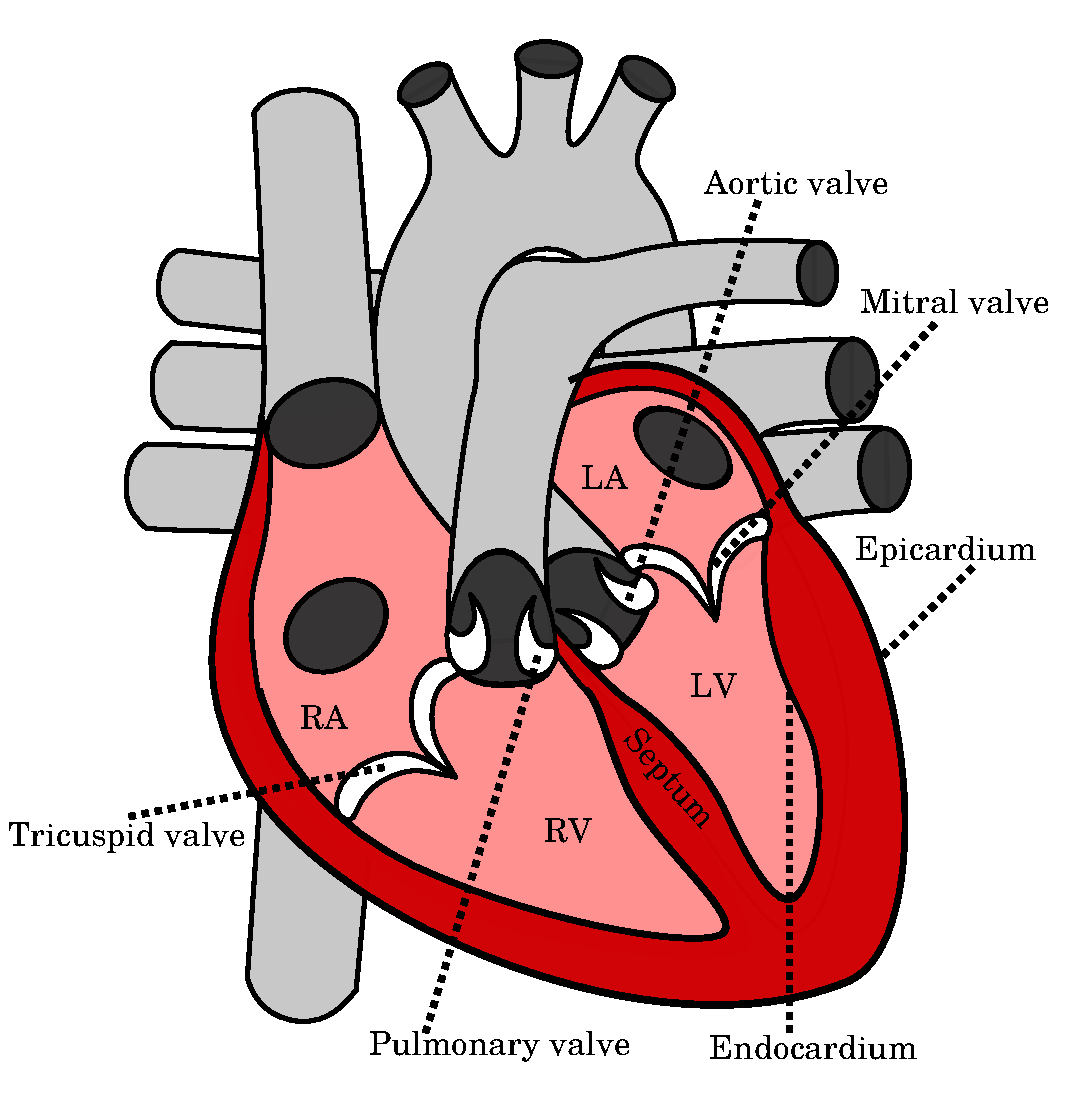
\includegraphics[width=0.7\textwidth]{chapters/introduction/figures/heart_anatomy.pdf}
\caption{Schematic representation of the heart's anatomy. (Adapted and modified from Wapcaplet in Sodipodi).}
\label{fig:heart_anatomy}
\end{figure}


Deoxgenated blood is transported from the body through the veins and to
the right atrium (RA). From the RA, blood flows to the right ventricle
(RV), before it is sent through the the pulmonary arteries(PA) and to the
lungs, where the bloods gets oxygenated. From the lungs, the blood
travels through the pulmonary veins to the left atrium (LA), and
finally to the left ventricle (LV), before is is sent out to the body
again through the aorta.

The heart itself is located approximately in the center of the chest
with the \emph{apex} of heart angled down towards the left of the
body, and the \emph{base} located just behind the breastbone.


Starting from the outside of the heart we have the \emph{pericardium},
the \emph{epicardium}, the \emph{myocardium} and the \emph{endocardium}. 
The pericardium is a fibroserous sac that surrounds that heart, and
the endo- and epicardium are respectively the inner and outer layers
of the myocardium. The myocardium is made up by individual muscle cells, or
myocytes, which branch and join neighboring cells, and form a
complicated fibrous network which is often referred to as a 
\emph{functional syncytium} (meaning that the number of active muscle
fibers cannot be varied from beat to beat).

The ventricular muscle fibers orientations varies smoothly through the
wall, and rotates from the endocardium to the epicardium forming a
helical structure \cite{streeter1969fiber}. These muscle fiber are
further organized in laminar sheets, which is separated by gaps called
cleavage planes \cite{legrice1995laminar}.

Each myocyte is composed of bundles of myofibriles, which again contains
\emph{myofilaments}. The myofilaments consist of a repeated pattern
of lines and bands which can be seen as a collection of individual
contractile units called \emph{sarcomeres}. A simple sketch of a
sarcomere is shown in Figure \ref{fig:sarcomere}. 
\begin{figure}[htbp]
  \centering
    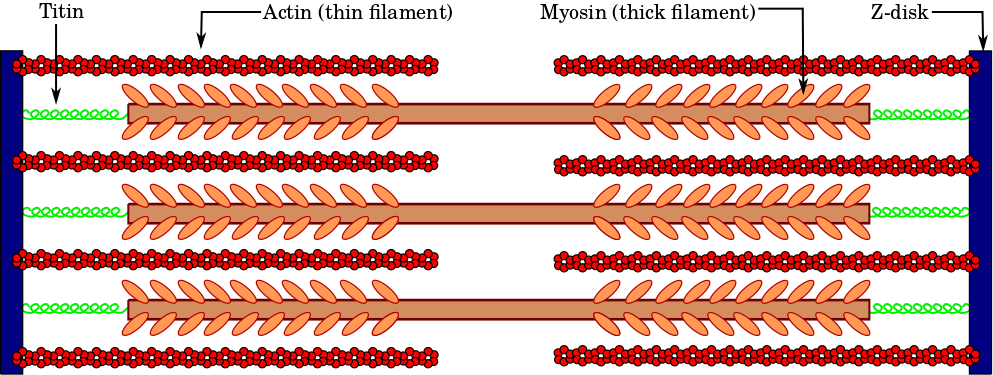
\includegraphics[width=1.0\textwidth]{chapters/introduction/figures/Sarcomere.png}
\caption{Illustration of the sarcomere structure.}
\label{fig:sarcomere}
\end{figure}

The sarcomeres are composed thick and thin filaments that slides
back and forth when the muscle contracts or relaxes.
The thin filaments are made up by a protein called \emph{actin} while
the thick filaments are made up by a protein called \emph{myosin}.



\subsection{The cardiac cycle}
\label{sec:cardiac_cycle}

The heart beats in a cyclic manner, about one beat every second.
The contraction of the heart is triggered by an action
potential originating from specialized cells in the right atrium. When an action
potential is triggered, calcium is released into the cells. These
calcium ions binds to a complex called troponin C located at the thin
filaments, which then exposes the actin to the myosin head. When
myosin binds to actin we say that a \emph{cross-bridge} is formed
between the thin and thick filaments. A \emph{power stroke} is
triggered after ATP hydrolysis, and the sarcomere shortens. 
The signal propagates through the myocardium and along
specialized electrical highways with high conducting cells.

% One way to describe the cardiac cycle is via the \emph{electrocardiogram}
% (ECG), which is a way of measuring the electrical propagation though
% the heart. Another
One way to describe the cardiac cycle is by means of
the pressure and volume inside the individual chambers. For example, plotting
the left ventricular (LV) volume on the $x-$axis and the LV pressure on the $y-$axis
provides an intuitive representation of the cardiac cycle known as the
\emph{PV-loop}. In Figure \ref{fig:pv_loop} we show an illustration of
a typical PV-loop. At end-diastole (ED), the mitral valve closes, and
the ventricle contracts against a rising pressure. During this phase,
no blood goes in or out of the ventricle and we call it the
\emph{isovolumic contraction} phase. When the
ventricular pressure exceeds the aortic pressure, the aortic valve
opens and the heart \emph{ejects} blood into the body. When the ventricular
pressure drops below the aortic pressure, the aortic valve closes and
pressure drops as the ventricle relaxes, and we enter the
\emph{isovolumic relaxation} phase. The phase when the ventricle
contracts, from end diastole until the end of ejection is called
\emph{systole}, hence this point in the cycle is also know as
end-systole (ES). Similarly, the phase for which the ventricle
relaxes from the beginning isovolumic relaxation to end diastole, is
called \emph{diastole}. When the pressure drops below the atrial pressure 
the mitral valve opens and blood is sucked into the ventricle. In the
final stage of the filling of the ventricle, the atria contracts and
fills the ventricle before we arrive at end-diastole, and the cycle
repeats. 


\begin{figure}[htbp]
  \centering
    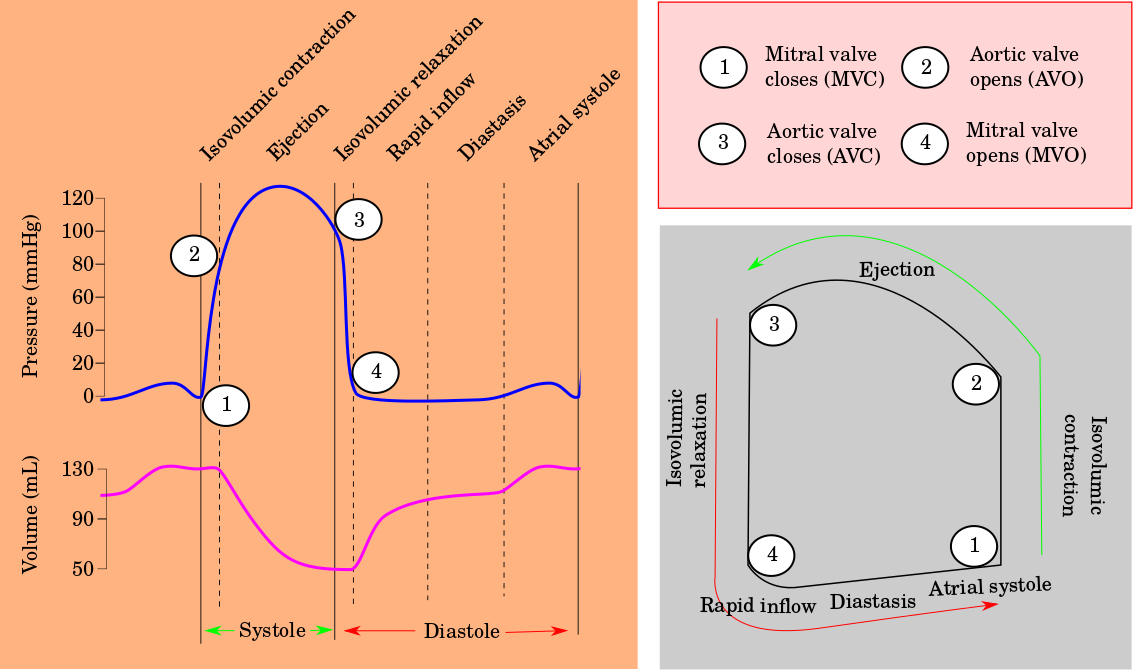
\includegraphics[width=0.85\textwidth]{chapters/introduction/figures/cardiac_cycle.png}
\caption{Showing the relation between pressure and volume in the left
  ventricle during the cardiac cycle. To the left we show a reduced version of
the classical Wiggers diagram with pressure and volume plotted against
time. To the right we show the pressure volume loop
with volume plotted on the $x-$axis and pressure on the $y-$axis. }
\label{fig:pv_loop}
\end{figure}


% A couple of terminologies used throughout 
\subsection{Ventricular pumping function}
\label{sec:ventricular_pumping_function}



The pressure and volume inside the ventricle can provide us with
information about the passive and active properties of the
myocardium. Imagine it was possible to shut down all contractile
units in the myocardium, and remove all loads (e.g set the pressure
to zero). This would be analogous to have a deflated balloon. In order to
get some information about the stiffness of the myocardium one could
try to inflate the ventricle. The stiffer the myocardium is, the
higher pressure would be needed in order to increase the volume.
This relationship between the pressure and volume during the inactive
state is called the end diastolic pressure volume relationship
(\emph{EDPVR}).

Similarly, imagine now that the ventricle is at the end-systolic state,
when the muscle cells are contracting at their most forcefully. Changing
the pressure at this state would also result in a change in volume and
this relationship between pressure and volume  is called the end
systolic pressure volume relationship (\emph{ESPVR}). The two pressure
volume relationships are depicted in Figure \ref{fig:intro_pvr}.

\begin{figure}[htbp]
  \centering
    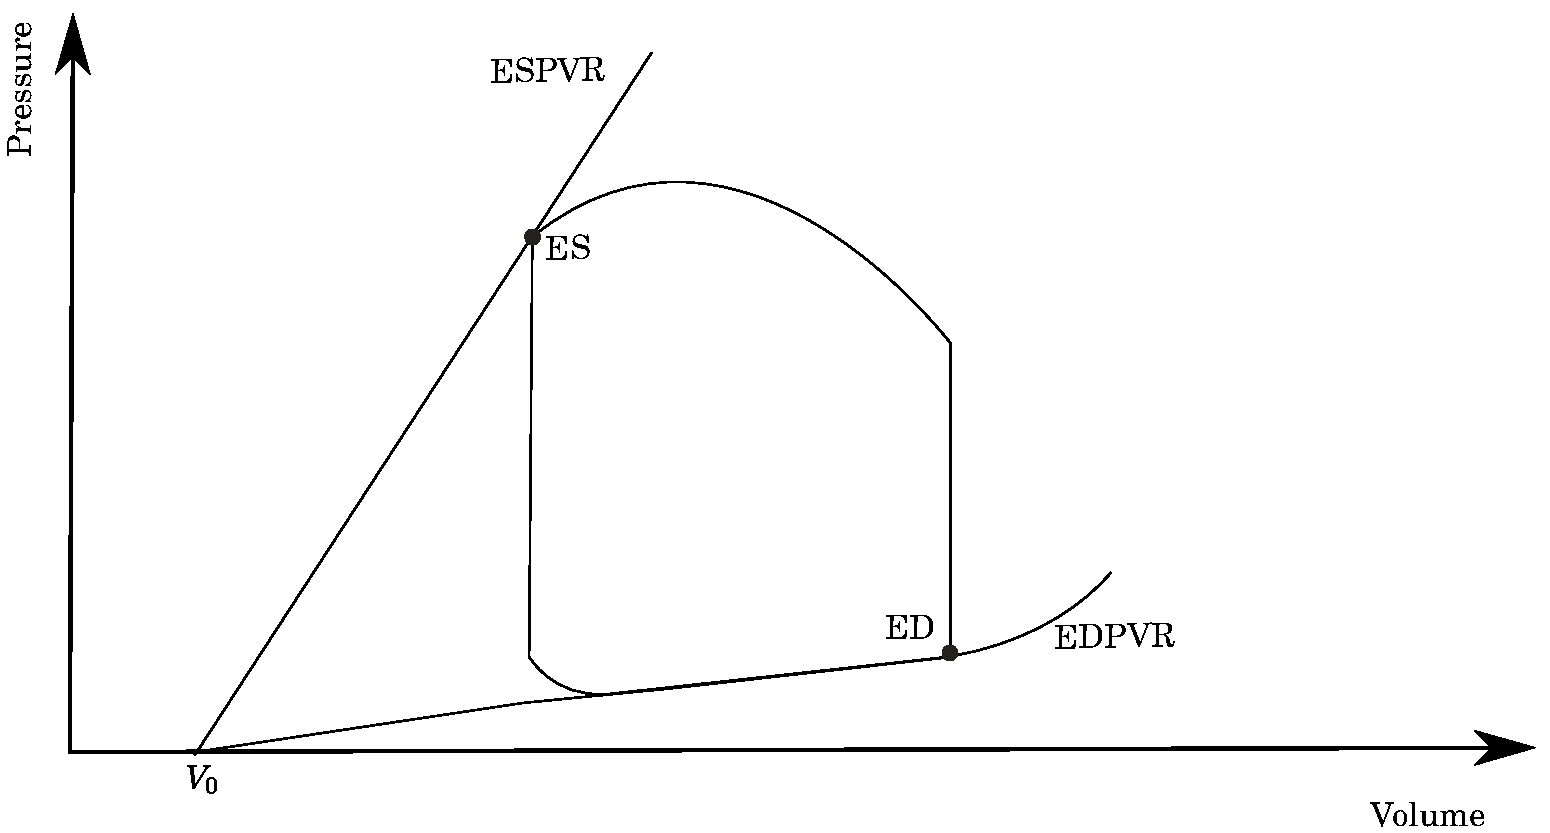
\includegraphics[width=\textwidth]{chapters/introduction/figures/pvr.pdf}
\caption{Illustration of the end diastolic pressure volume
  relationship (EDPVR) and the end systolic pressure volume
  relationship (ESPVR). The volume axis intercept $V_0$ from the time
  varying elastance model is also shown. }
\label{fig:intro_pvr}
\end{figure}




Although single-beat estimation of these relationships do
exist \cite{senzaki1996single,klotz2006single}, the EDPVR and ESPVR
can be estimated by changing the loading condition.
Changing the \emph{preload}, i.e the load on the ventricle
before it starts contracting would brings us along the EDPVR
curve, while changing the \emph{afterload}, i.e the load after
the ventricle has contracted, would shift the end-systolic point along
the ESPVR curve.


The ventricular pumping function depends on the loads that the
ventricle experience. If the amount of blood returning from the veins
into the heart increases, i.e increased preload, the end diastolic
volume increases and the ventricle contracts more forcefully in order
to synchronize the amount of ejected blood with the venous
return. This fundamental law, is called the \emph{Frank-Starling
  law}. The Frank-Starling law relates the EDPVR to the ESPVR, and
states that the stroke volume, i.e the difference in end systolic and
end diastolic volume, increases in response to and increase in
preload. This allows the cardiac output to
be synchronized with the venous return and blood supply, without
depending upon external regulation. 


The slope of any pressure volume relationship is called the \emph{elastance},
and a famous model known as the  time varying elastance model, relates
the cavity pressure in the ventricle to the volume and a time varying elastance $E(t)$
\cite{sagawa1977end},  
\begin{align}
  P(t) = E(t)( V(t) - V_0 ).
  \label{eq:time_varying_elastance}
\end{align}
Here $P$ is the endocardial pressure, $V$ the cavity volume, $E$ the
time-varying elastance, and $V_0$ the volume axis intercept.

In fact, the end systolic elastance, $E(t)$ with $t$ being time of end
systole, is considered to be the gold
standard in terms of quantifying myocardial \emph{contractility}.
However, it is rarely used because it is difficult to determine
clinically. What should be noted is that end systolic elastance is
independent of load, and therefore serves as measure of the ability of
the ventricle to do work, i.e myocardial contractility.







% 



% % The Starling Curve is a plot of the ESPVR - EDPVR, showing that the
% % output increases up to some maximum (at the ascending limb). Thereafter
% % it decreases on the descending limb. If the sarcomeres works on the
% % descending limb, the heart would dilate and become weakened.


% Stroke volume, cardiac output. 







% \subsection{Myocardial Contractility}

% Contractility can be seen as the manifestation of all the factors that
% influence the interactions between the contractile proteins.
% One simple definitions is \emph{myocardial contractility is the
%   ability of the heart to do work}. A change in myocardial
% contractility can be seen if there is a change in ejection which is
% not caused by changes in the initial fiber length (ED). If the end
% diastolic volume remains the same, but the stroke work changes there
% is a change in contractility.

% Under normal circumstances, the myocardial cells generate less than
% half the of their maximal contractility. One could increase the
% contractility by providing more calcium to the cells.


% In order to find a suitable index for myocardial contractility we take
% step back and consider Hills postulate: \emph{the ``active points'' of
%   muscle can exist in two states: 1. active points are maintaining
%   tension, 2. the active points are participating in a chemical
%   reaction.} 
% If the muscle is presented with a heavy load, developed tension is
% high, shortening velocity is low and the load is only moved a short
% distance. In this case the active points are holding tension.
% On the other hand, if the muscle is presented with a light load, the
% shortening velocity is high and the load is moved a longer
% distance. In this case more of the active points are participating in
% chemical reactions. 
% In both cases, the contractility might be the same which is why we
% need a load independent measure of contractility.
% Looking at the force-velocity relationship we can say that the maximum
% force (tension) is achieved when all the active points are holding
% tension ($P_0$). $P_0$ is proportional to the number of active
% cross bridges.
% Similarly, the maximum velocity is achieved when all
% the active points are participating in a chemical reaction
% ($V_{\text{max}}$). $V_{\text{max}}$ reflects the maximal rate of
% cross bridge cycling. 
% This is explained by the Hill equation, which
% relates the force to velocity, and the intercepts are $P = P_0, (V = 0)$
% and $V = V_{\text{max}}, (P = 0)$. This is very difficult to meause in
% cardiac cells because cariac muscle cells are not tentanized.

% The most commonly used index of contractility was formalized
% \cite{sagawa1977end} using a time varying elastance model, which
% states that at any point in the cardiac cycle the pressure and volume
% are linearly related by the time-varying elastance, or formally:
% \begin{align}
%   P(t) = E(t)( V(t) - V_0 ).
%   \label{eq:time_varying_elastance}
% \end{align}



\subsection{Cardiac Pathophysiology}
Pathophysiology is the study of the physiology of the diseased heart,
and we will briefly mention some of the different cardiac diseases
encountered in this thesis. 


\subsubsection{Heart failure}
Heart failure (HF) is a common term for all heart diseases in which the
heart is unable to supply the body with enough blood to meet its
demand. It is common to separate between diastolic and systolic HF.
Diastolic HF refers to the heart's inability to be passively
filled, and thereby reduce the cardiac output according to the 
Frank-Starling law of the heart. In systolic HF on the other had, the
heart's ability to contract efficiently is reduced.

% Consequently, patients suffering from heart failure has a reduced
% cardiac output. It is common to distinguish between systolic and
% diastolic heart failure. 

\subsubsection{Left bundle branch block}

One type of heart failure can result from conduction block in the
heart. An electrical wave travels through electrical highways
of high conducting cells. One of these highways known as the Bundle of
His splits into two parts, the right and left bundle. The right bundle
activates the right ventricle, while the left bundle activates the
left ventricle. For patients suffering from left bundle branch block,
there is ``road block'' on the highway along the left bundle, meaning
that the left ventricle is activated later than preferable, and the
right ventricle is activated prior to the left
ventricle. This can result in a dyssynchronous contraction, yielding a
reduced pumping effect. A promising treatment for these patients is
called Cardiac Resynchronization Therapy (CRT) \cite{cleland2005effect}.

Imagine a boat with rowers on both sides trying to get the boat moving
forward. If the rowers don’t synchronize their strokes, the boat will
veer from side to side and have a much longer route – if it gets
anywhere at all. To synchronize the rowers, we could add a coxswain
who tells the rowers when to row. We can use the rower analogy to
think of the contractions of the left and right side of the
heart. With the heart, implanting a CRT device is like adding a
coxswain to direct the rowers. The CRT’s goal is to try to
resynchronize the heart so that the left and right ventricles contract
simultaneously. It involves pacing the heart on both the left and
right ventricle so that the heart can contract in a synchronous
way. Therefore CRT is often referred to as biventricular pacing, or
just BiV pacing. However, experiments show that between 30-40\% of the
selected patients do not respond to CRT \cite{daubert20122012}, which
is why much research is put into increasing the responder rate. 



% \subsubsection{Pulmonary hypertension}


\subsection{Summary of Cardiac Physiology}
The multiscale and multiphysics phenomena governing the mechanics of
the heart is complex. How the molecular dynamics should be coupled to
the electrophysiology at the cellular level, how the electrophysiology
should be coupled to the mechanics at the organ level and what type of
feedback mechanisms that should be included is far from fully
understood. In this thesis we limit ourselves to the study of what is
happening on the organ level, and concentrate purely on the mechanical
aspect. 


%%% Local Variables:
%%% mode: latex
%%% TeX-master: "../../main"
%%% End:

\newpage
\section{Mechanical modeling}
\label{sec:intro_mechanical}

In this section we will cover the necessary theory of continuum
mechanics in order to model the mechanics of the heart. The theory of
continuum mechanics is extensive, and we will not be able to cover
everything. For a complete review of continuum mechanics the reader is
therefore referred the textbook of Gerhard Holzapfel
\cite{holzapfel2000nonlinear} from which most of the theory in this
section is taken. For the even more mathematically oriented reader we
refer to \cite{marsden1994mathematical}.

\subsection{Kinematics}
We represent the heart as a continuum body $\mathfrak{B}$ embedded in
$\mathbb{R}^3$. A configuration of $\mathfrak{B}$ is a mapping $\chi:
\mathfrak{B} \rightarrow \mathbb{R}^3$. 
We denote the \emph{reference configuration} of the heart by $\Omega
\equiv \chi_0(\mathfrak{B})$, and the \emph{current configuration} by $\omega
\equiv \chi(\mathfrak{B})$. The mapping $\varphi :  \Omega
\rightarrow \omega$, given by the composition $\varphi = \chi
\circ \chi_0^{-1}$, is a smooth, orientation preserving (positive
determinant) and invertible map. We denote the coordinates in the
reference configuration by $\Xvec \in \Omega$, and the coordinates in the current
configuration by $\xvec \in \omega$. The coordinates $\Xvec$ and $\xvec$ are
commonly referred to as material and spatial points respectively, and
are related through the mapping $\varphi$, by $\xvec = \varphi(\Xvec)$.
For time-dependent problems it is common to make  the time-dependence
explicitly by writing $\xvec = \varphi(\Xvec, t)$. In the following
we will only focus on the mapping between two configurations and
therefore no time-dependence is needed. The \emph{deformation gradient} is a
rank-2 tensor, defined as the partial derivative of $\varphi$  with
respect to the material coordinates:
\begin{align}
  \F = \nabla_{\Xvec} \varphi= \Grad \xvec.
  \label{eq:deformation_gradient}
\end{align}
Here we also introduce the notation $\Grad$, which means derivative
with respect to reference coordinates.
The deformation gradient maps vectors in the reference configuration to
vectors in the current configuration, and belongs to the space of
linear transformations from $\mathbb{R}^3$ to $\mathbb{R}^3$ with
strictly positive determinant, which we denote by
$\mathrm{Lin}^+$. Another important quantity is the
\emph{displacement} field  
\begin{align}
  \uvec = \xvec-\Xvec, 
  \label{eq:displacement}
\end{align}
which relates positions in the reference configuration to positions
in the current configuration. From \eqref{eq:deformation_gradient} we
see that
\begin{align}
  \F = \Grad \xvec = \Grad \uvec + \Grad \Xvec = \Grad \uvec + \I.
\end{align}

Some other useful quantities are the \emph{right Cauchy-Green} deformation
tensor $\C = \F^T\F$, the \emph{left Cauchy-Green} deformation tensor
$\mathbf{B} = \F\F^T$, the \emph{Green-Lagrange} strain tensor
$\mathbf{E} = \frac{1}{2}(\C - \I)$, and the determinant of the
deformation gradient $J = \det \F$.

An important concept in mechanics is the concept of stress, which is
defined as force per area
$\left[\frac{\mathrm{N}}{\mathrm{m}^2}\right]$. When working with
different configurations one needs to be careful with which forces and
which areas we are talking about. Table \ref{tab:stress_tensor}
shows how forces and areas are related for the most important stress
tensors used in this thesis. Note that the explicit form of the stress
tensor requires a constitutive law for the material at hand. This will
be discussed in more detail in Section \ref{sec:constitutive_relations}.

\begin{table}[h]
  \centering
  \begin{tabular}{lll}
    \toprule
    Stress tensor & Forces & Area \\
    \midrule
    Second Piola-Kirchhoff ($\SPK$) & Reference configuration & Reference configuration \\
    First Piola-Kirchhoff ($\FPK$) & Current configuration  &  Reference configuration \\
    Cauchy ($\Cauchy$) &  Current configuration & Current configuration  \\
    \bottomrule
  \end{tabular}
  \caption{\label{tab:stress_tensor}Showing different stress tensors
    used in this thesis, and how
    they relate forces to areas trough different configurations.}
\end{table}


\subsection{Balance laws and transformations}
In this section we will cover some basic transformations used to
derive the fore-balance equations for the mechanics of the heart. 

\subsubsection{Transformations between reference and current
  configuration}
By definition, the reference configuration $\Omega$, and current
configuration $\omega$, are related via the deformation map $\varphi$ in the
sense that a point $\mathfrak{p} \in \mathfrak{B}$ with reference
coordinates $\Xvec$ and current coordinates $\xvec$ satisfies $\xvec =
\varphi(\Xvec)$. Likewise a vector in the reference configuration is
related to a vector in the current configuration  via the
deformation gradient $\F$; if $\mathrm{d}\Xvec$ is a vector in the
reference configuration it will transform to the vector
$\mathrm{d}\xvec$ in the current configuration, and $\mathrm{d}\xvec =
\F \mathrm{d}\Xvec$. From this relation we also derive that the
transformation of an infinitesimal volume element in the reference
configuration, $\mathrm{d}V$ is related to an infinitesimal volume
element in the current configuration, $\mathrm{d}v$  via the determinant of the
deformation gradient,
\begin{align}
  \mathrm{d}v =\det(\F) \mathrm{d}V.
  \label{eq:volume_element}
\end{align}
Another important transformation is the transformation of normal
vectors. By noting that we can write \eqref{eq:volume_element} using
surface elements
\begin{align*}
  \mathrm{d}s \mathbf{n} \mathrm{d}\xvec  &= \mathrm{d}v = \det(\F) \mathrm{d}V = \det(\F) \mathrm{d}S  \Nvec \mathrm{d}\Xvec\\
  &\implies \left( \mathrm{d}s \mathbf{n} \F  - \mathrm{d}S \det(\F) \Nvec \right) \mathrm{d}\Xvec = 0\\
  &\implies \left( \mathrm{d}s \F^T \mathbf{n}  - \mathrm{d}S \det(\F) \Nvec \right) \mathrm{d}\Xvec = 0,\\
\end{align*}
we get \emph{Nanson's formula}
\begin{align}
  \mathrm{d}s \mathbf{n}  =  \det(\F) \F^{-T} \mathrm{d}S \Nvec,
\end{align}
which relates the normal vector in the current configuration to the
normal vector in the reference configuration.


\subsubsection{Conservation of linear momentum}
Newton's seconds law states that the change in linear momentum equals
the net impulse acting on it. For a continuum material with constant
mass density $\rho$ this implies that
\begin{align}
  \int_{\omega} \rho \dot{\mathbf{v}} \mathrm{d}v = \mathbf{f},
  && \mathbf{f} = \int_{\partial \omega} \mathbf{t} \mathrm{d}s
     + \int_{\omega} \mathbf{b} \mathrm{d}v,
     \label{eq:cons_lin_mom}
\end{align}
where $\mathbf{v}$ is the spatial velocity field, $\mathbf{t}$ is
the traction acting on the boundary, and $\mathbf{b}$ is the body
force. From \emph{Cauchy's stress theorem} we know that there exists a
second order tensor $\sigma$, known as the Cauchy stress tensor that is
related to the traction vector by $\mathbf{t} = \sigma \mathbf{n}$,
where $\mathbf{n}$ is the unit normal in the current configuration.
Using the divergence theorem we get
\begin{align*}
  \int_{\partial \omega} \mathbf{t} \mathrm{d}s
  = \int_{\partial \omega} \sigma \mathbf{n} \mathrm{d}s
  = \int_{\omega} \nabla \cdot \sigma \mathrm{d}v,
\end{align*}
and by collecting the terms from \eqref{eq:cons_lin_mom} we arrive at
Cauchy's momentum equation
\begin{align}
  \nabla \cdot \sigma + \mathbf{b} =  \rho \dot{\mathbf{v}}.
  \label{eq:chauch_momentum_eq}
\end{align}
The contribution from the body force ($\mathbf{b}$)  and inertial term
($\rho \dot{\mathbf{v}}$) can be considered negligible compared to the stresses
\cite{hunter1996kd,tallarida1970left, moskowitz1981effects}, which is
why the force balance equations is typically only stated as
\begin{align}
  \nabla \cdot \sigma = \mathbf{0}.
  \label{eq:momentum_simple_current}
\end{align}
Note that we have formulated the balance law in the current
configuration. An equivalent statement can be formulated in terms of
the reference configuration
\begin{align}
  \nabla \cdot \FPK = \mathbf{0}, 
  \label{eq:momentum_simple_reference}
\end{align}
where $\FPK$ is the first Piola-Kirchhoff stress tensor. Note that the
operator $\nabla \cdot$ acting on the Cauchy stress tensor represents
differentiation with respect to coordinates in the current
configuration, while when acting on the first Piola-Kirchhoff stress
tensor represent differentiation with respect to coordinates in the
referece configuration. 

\subsubsection{Conservation of angular momentum}
Just like linear momentum, the angular momentum is also a conserved
quantity. We will not go through the derivation, but state that as a
consequence, the Cauchy stress tensor is symmetric
\begin{align}
  \sigma = \sigma^T.
\end{align}



\subsection{Hyperelasticity}
\label{sec:hyperelasticity}

Even though experimental studies have indicated visco-elastic behavior
of the myocardium \cite{dokos2002shear, gultekin2016orthotropic}, a
common assumption is to consider quasi-static behavior, meaning that
the inertial term in \eqref{eq:chauch_momentum_eq} is negligible and
static equilibrium is achieved at all points in the cardiac cycle. Therefore
it is also possible to model the myocardium as a hyperelastic
material,which is a type of elastic material. 
This means that we postulate the existence of
a strain-energy density function $\Psi:\mathrm{Lin}^+ \rightarrow
\mathbb{R}^+$, and that stress is given by the relation
\begin{align}
\FPK = \frac{\partial \Psi(\F)}{\partial \F}.
\end{align}
Since stress has unit Pa, we see that the strain-energy density
function is defined as energy per unit reference volume, and has units
$\frac{\text{Joule}}{m^3}$. 
The strain-energy density function relates  the amount of
energy that is stored within the material in response to a given
strain. Hence, the stresses in a hyperelastic material with a given
strain-energy density function, depend only on the strain, and not the
path for which the material deforms. On the contrary, if the model had
been visco-elastic we would expect to see hysteresis in the
stress/strain curve, but this is not possible for a hyperelastic
material. 

\begin{remark}
  The second law of thermodynamics states that the total entropy
  production in a thermodynamic process can never be negative. Elastic
  materials define a special class of materials in which the entropy
  production is zero. Within this thermodynamic framework the
  strain-energy density function coincides (up to a constant) with the
  Helmholtz free energy density.
\end{remark}


\subsubsection{General requirements for the strain-energy density
  function}
\label{sec:strain_energy_req}
Some general requirements must hold for the strain-energy function.
First of all, we require that the reference state is stress free and
that the stored energy increases monotonically with the deformation. 
Formally this can be stated simply as 
\begin{align*}
  \Psi(\I) = 0 \; && \text{and} &&\; \Psi(\F) \geq 0.
\end{align*}
Moreover, expanding or compressing a body to zero volume would
require an infinite amount of energy, i.e
\begin{align*}
  \Psi(\F) \rightarrow \infty \; && \text{as} &&\; \det \F \rightarrow& 0 \\
  \Psi(\F) \rightarrow \infty \; && \text{as} &&\; \det \F \rightarrow& \infty
\end{align*}
We say that the strain energy should be objective, meaning that the
stored energy in the material should be invariant with respect to
change of observer. Formally we must have: \emph{given any positive symmetric
rank-2 tensor $\C \in \mathrm{Sym}$:}
\begin{align}
  \Psi(\mathbf{C}) = \Psi(\mathbf{Q}\mathbf{C}\mathbf{Q}^T), \; \forall \mathbf{Q} \in \mathcal{G} \subseteq \mathrm{Orth}.
\end{align}
Here $\mathrm{Orth}$ is the group of all positive orthogonal matrices.
If $\mathcal{G} = \mathrm{Orth}$ we say that the material is
isotropic, and otherwise we say that the material is anisotropic.
This brings us to another important issue, which is related to the
choice of coordinate-system. Having to deal with different
coordinate-systems, and mapping quantities from one coordinate-system
to another can results in complicated computations. Therefore it would be beneficial if we
could work with quantities which do not depend on the choice of
coordinate-system. Such quantities are called invariants. 
If the material is isotropic, the representation theorem for
invariants states that $\Psi$ can be expressed in terms of the
principle invariants of $\mathbf{C}$, that is $\Psi = \Psi(I_1, I_2,
I_3)$. The principle invariants $I_i, i=1,2,3$ are the coefficients in
the characteristic polynomial of $\mathbf{C}$, and is given by 
\begin{align}
  I_1 = \tr \C,  && I_2 = \frac{1}{2}\left[ I_1^2 - \tr(\C^2)\right] && \text{and} && I_3 = \det \C.
\end{align}
In the case when the material constitutes a transversely isotropic
behavior, that is, the material has a preferred direction $\mathbf{a}_0$,
which in the case of the myocardium could be the direction of fiber
muscle fibers, we have
\begin{align*}
  \mathcal{G} = \{ \mathbf{Q} \in \mathrm{Orth}: \mathbf{Q}(\mathbf{a}_0\otimes\mathbf{a}_0)\mathbf{Q}^T = \mathbf{a}_0\otimes\mathbf{a}_0 \},
\end{align*}
with $\otimes$ being the outer product. In this case the strain-energy
density function can still be expressed through invariants. However,
we need to include the so called quasi-invariants, which are defined
as stretches in the local microstructural coordinate-system. The
transversely isotropic invariants are given by
\begin{align*}
  I_{4\mathbf{a}_0 } = \mathbf{a}_0 \cdot (\C \mathbf{a}_0) && \text{and} && I_5 = \mathbf{a}_0 \cdot (\C^2 \mathbf{a}_0).
\end{align*}
Some of the invariants do have a physical interpretation. For instance, $I_3$
is related to the volume ratio of material during deformation, while
$I_{4\mathbf{a}_0 } $ is related to the stretch along the direction
$\mathbf{a}_0 $. Indeed the \emph{stretch} ratio in the direction
$\mathbf{a}_0$ is given by $\lambda_{\mathbf{a}_0} = | \F \mathbf{a}_0
|$ and we see that $I_{4\mathbf{a}_0 }  =  \mathbf{a}_0 \cdot (\C
\mathbf{a}_0) = \F \mathbf{a}_0 \cdot (\F \mathbf{a}_0) =
\lambda_{\mathbf{a}_0}^2$. For more details about invariants see e.g
\cite{holzapfel2009constitutive,liu1982representations}.


The theory of global existence of unique solutions for elastic problems
was originally based convexity of the free energy function.
An energy function $\Psi: \mathrm{Lin}^+ \rightarrow
\mathbb{R}^+$ is strictly \emph{convex} if for each $\F \in
\mathrm{Lin}^+$ and $\mathbf{H} \neq \mathbf{0}$ with $\det (\F +
(1-\lambda)\mathbf{H}) > 0$, we have
\begin{align}
  \Psi(\lambda \F + (1-\lambda) \mathbf{H})
  < \lambda \Psi(\F)
  + (1-\lambda) \Psi(\F + \mathbf{H}), && \lambda \in (0,1).
\label{eq:strain_convex}
\end{align}
If the response $\FPK$ is differentiable, then condition
\eqref{eq:strain_convex} is equivalent of saying that the response is
positive definite, 
\begin{align}
  \mathbf{H} : \frac{\partial \FPK}{\partial \F} : \mathbf{H} > 0,
  && \F \in
     \mathrm{Lin}^+, \mathbf{H} \neq \mathbf{0}.
\label{eq:response_posdev}
\end{align}

However, from a physical point of view this requirement is too strict
\cite{ball1976convexity}. A slightly weaker requirement is the strong
ellipticity condition which states that \eqref{eq:response_posdev}
should hold for any $\mathbf{H}$ of rank-one, and is analogous to
say that the strain energy function is rank-one convex. 

% that the
% strain-energy function $\Psi$ is \emph{polyconvex}, meaning that there exist
% a convex function $\phi$ such that
% \begin{align*}
%   \Psi(\F) = \phi(\F, \cof \F, \det \F).
% \end{align*}
% Note however, that if $\Psi$ is convex then it is also polyconvex.


% \subsubsection{Work conjugates}


% \begin{table}[h]
%   \centering
%   \begin{tabular}{ll}
%     \toprule
%     Stress & Strain \\
%     \midrule
%     Second Piola ($\SPiola$) & Green Lagrange ($\mathbf{E}$) \\
%     First Piola ($\FPiola$) & Deformation gradient ($\mathbf{F}$) \\
%     Cauchy ($\mathbf{\sigma}$) &  Eulerian-Almansi ($\mathbf{e}$) \\
%     \bottomrule
%   \end{tabular}
%   \caption{\label{tab:work_conjugates}Work conjugate stress-strain pairs}
% \end{table}

% By conjuagate stress-strain paris we mean that the rate of mechanical
% work is given by the stress times the strain-rate. For example,
% the total work per unit volume done by the stresses from time $t_1$ to
% $t_2$ is given by
% \begin{align}
%   \mathcal{W}(t_1, t_2) &=  \int_{t_1}^{t_2} \mathbf{P} : \dot{\F} dt
%                           = \int_{t_1}^{t_2} \frac{\partial \Psi (\F)}{\partial \mathbf{F}}  : \dot{\F} - p \F^{-T} :  \dot{\F}  dt \\
%                         &= \int_{t_1}^{t_2} \frac{D \Psi (\F)}{D t} - p\cdot 0 dt
%                           = \Psi(\F(t_2)) - \Psi(\F(t_1)).
% \end{align}
% Note that this is a measure of work per unit volume.


\subsection{Incompressibility}
\label{sec:incompressibility}

The myocardium contains small blood vessels that supply the
myocardial cells with oxygen. When the myocardium contracts, this
perfused blood is squeezed out, resulting in an overall loss of
2-4\% volume\cite{yin1996compressibility}. A material that change its
volume in response to applied loads are referred to as compressible. When the 
volume is preserved we refer to the material as incompressible.
Since 2-4\% is very little, a common assumption in cardiac mechanical modeling,
which has also been made in the work conducted in this thesis, is to assume
the myocardium to be incompressible. The reason for this choice is
purely numerical.

For an incompressible material, only isochoric motions are
possible. This means that the volume of the material does not change during
any deformation, and hence we have the constraint 
\begin{align}
  J = \det(\F) = 1.
  \label{eq:incompressible_cons}
\end{align}
The constraint \eqref{eq:incompressible_cons} can be imposed by
considering the modified strain energy function
\begin{align}
  \Psi = \Psi(\F) + p(J-1),
  \label{eq:incomp_strain_energy}
\end{align}
where $p$ is a scalar which serves as a Lagrange multiplier, but which
can be identified as the hydrostatic pressure. If we differentiate
\eqref{eq:incomp_strain_energy} with respect to $\F$ we get the First
Piola-Kirchhoff stress tensor for an incompressible material
\begin{align}
  \FPK = \frac{\partial \Psi(\F)}{\partial \F} + J p \F^{-T}.
\end{align}
Likewise the Cauchy stress tensor is given by
\begin{align}
  \Cauchy = J^{-1} \frac{\partial \Psi(\F)}{\partial \F}\F^{T} + p \I.
  \label{eq:cauchy_incomp}
\end{align}


\begin{remark}
  The sign of $p$ is determined by whether you add or subtract the term
  $ p(J-1)$ to the total strain energy in
  \eqref{eq:incomp_strain_energy}. For all practical purposes, it
  does not matter if you add or subtract the term as long as you are
  consistent. 
\end{remark}


\subsubsection{Uncoupling of volumetric and isochoric response}
The total strain energy function in \eqref{eq:incomp_strain_energy}
can be written as a sum of isochoric and volumetric components. Let
\begin{align}
  \F =  \F_{\mathrm{vol}} \F_{\mathrm{iso}},
\end{align}
then $ \F_{\mathrm{vol}} =
J^{1/3}\I$ and $\F_{\mathrm{iso}} = J^{-1/3}\F$. For
compressible materials (i.e with $J \neq 1$) it is important to consider
only deviatoric strains in the strain-energy density function, so that
$\Psi = \Psi_{\mathrm{iso}}(\F_{\mathrm{iso}}) +
\Psi_{\mathrm{vol}}(J)$. For incompressible material ($J = 1$), we
have $\F_{\mathrm{vol}} = \I$ so that such a decomposition seems
unnecessary. However, a similar decomposition has shown to be
numerically beneficial \cite{weiss1996finite}. Note that, in this case, a similar
decoupling of the stress tensors has to be done.

\subsection{Boundary Conditions}
\label{sec:mech_boudary}


Choosing the correct boundary conditions for the model is essential,
and the choice should mimic what is observed in reality. To
physiologically constrain the ventricle in a correct way is difficult,
and different approaches has been proposed.
The boundary condition at the endocardium is typically modeled as a
Neumann boundary condition, representing the endocardial blood
pressure. For the left ventricle we have
\begin{align}
  \sigma \mathbf{n} = -p_{\mathrm{lv}} \mathbf{n}, \;  \xvec \in  \lVendoCur, 
\end{align}
and for the right ventricle, ``lv'' is substituted with ``rv''.
This condition has a negative sign because the unit normal
$\mathbf{N}$ is pointing out of the domain, while the pressure is
acting into the domain. 
Note that this condition is imposed on the current configuration, and
to utilize the Lagrangian formulation we can pull back this condition
to the reference configuration to obtain
\begin{align}
  \FPK\mathbf{N} &= -p_{\mathrm{lv}} J\mathbf{F}^{-T} \cdot \mathbf{N}, \;  \Xvec \in \lVendo
\end{align}
Likewise, it is common to enforce a
Neumann boundary condition on the epicardium,
\begin{align}
\FPK\mathbf{N}  &= -p_{\mathrm{epi}}  J\mathbf{F}^{-T} \cdot \mathbf{N}, \;  \Xvec \in \epi.
\end{align}
However, the pressure $p_{\mathrm{epi}}$ is often set to zero as a
simplification. 

There exist a variety of boundary conditions at the base.
It is common to constrain the longitudinal motion of
base, even though it is observed in cardiac images that the apex tend
to be more fixed than the base. A recent study shows that taking into
account the base movement is important to capture the correct
geometrical shape \cite{palit2016passive}. However, this has not been
done in the studies in this thesis.
Fixing the longitudinal motion at the base is enforced through a
Dirichlet boundary condition,
\begin{align}
  u_1 = 0,  \;  \Xvec \in \lvbase,
\end{align}
where $u_1$ is the longitudinal component of the displacement $\uvec =
(u_1, u_2, u_3)$. To apply this type of condition, it is easiest if
the base is flat and located at a prescribed location, for example in
the $x= 0$ plane. Constraining the longitudinal motion of the base
alone is not enough since the ventricle is free to move in the basal
plane. In order to anchor the geometry it is possible to fix the
movement of the base in all directions
\begin{align}
  \uvec = \mathbf{0},  \;  \Xvec \in \lvbase,
\end{align}
or fixing the endocardial or epicardial ring
\begin{align}
  \uvec &= \mathbf{0},  \;  \Xvec \in \Gamma_{\mathrm{endo}} \\
  \uvec &= \mathbf{0},  \;  \Xvec \in \Gamma_{\mathrm{epi}}.
\end{align}

Another approach which is used in this thesis is to impose a Robin
type boundary condition at the base
\begin{align}
  \FPK \Nvec + k \uvec = \mathbf{0},  \;  \Xvec \in \lvbase, 
\end{align}
or at the epicardium to mimic the pericardium
\begin{align}
  \FPK \Nvec + k \uvec = \mathbf{0},  \;  \Xvec \in \lvepi.
\end{align}
Here $k$ can be seen as the stiffness of a spring that limits the
movement. The limiting cases, $k = 0$ and $k \rightarrow
\infty$ represent free and fixed boundary respectively.
More complex boundary conditions to mimic the pericardium are also
possible \cite{fritz2014simulation}, but not considered in this thesis.
An overview of the location of the different boundaries for the
bi-ventricular geometry is illustrated in Figure \ref{fig:boundaries}.

\begin{figure}[htbp]
  \centering
    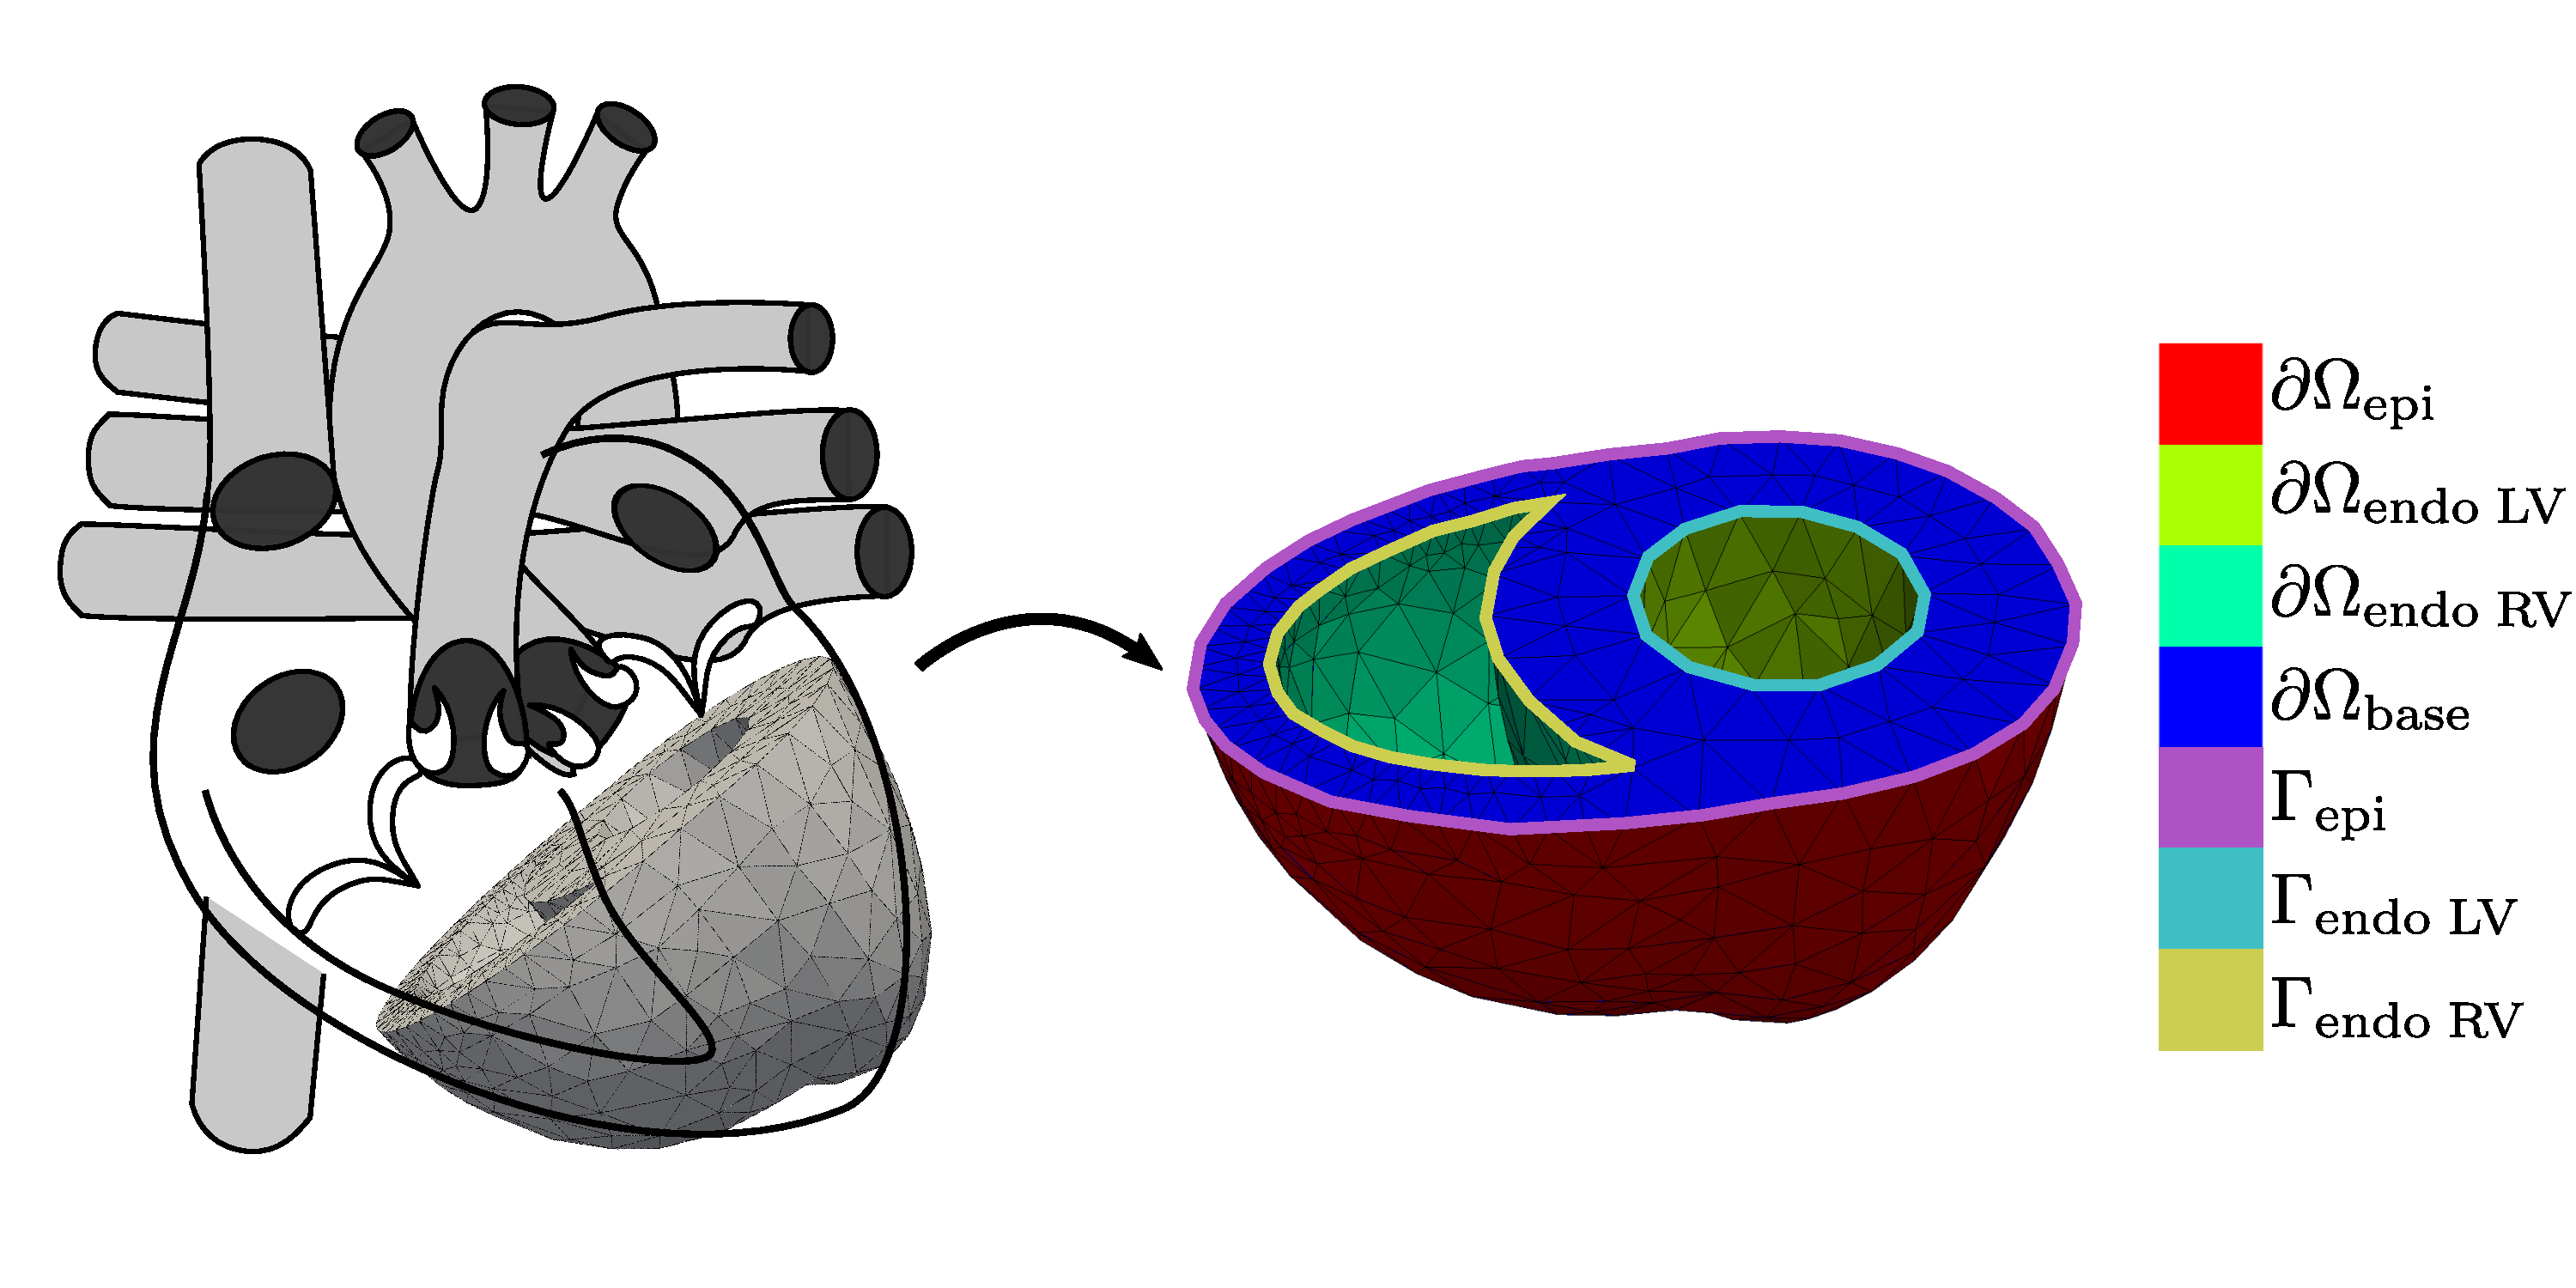
\includegraphics{chapters/introduction/figures/boundaries}
\caption{Illustration of the different boundaries in a bi-ventricular
  domain.}
\label{fig:boundaries}
\end{figure}


\subsection{Force-balance equation}
We will now collect all the terms that are involved in the force balance for
the cardiac mechanics problem. Considering the myocardium as an incompressible,
hyperelastic material we obtain the following strong form in the
Lagrangian formulation 
\begin{align}
  \begin{split}
  \nabla \cdot \FPK &= 0 \\
  J - 1 &= 0,
  \end{split}
 \label{eq:force_balance_strong}
\end{align}
completed with appropriate boundary conditions. To solve this
numerically using the finite element method, we need to derive weak
variational form of this equation.
% \begin{align}
%   \FPK \Nvec + k \uvec &= \mathbf{0},  \;  \Xvec \in \lvbase\\
%   u_1 &= 0,  \;  \Xvec \in \lvbase \\
%   \FPK\mathbf{N}  &= \mathbf{0}, \;  \Xvec \in \epi \\
%   \FPK\mathbf{N} &= -p_{\mathrm{lv}} J\mathbf{F}^{-T} \cdot \mathbf{N}, \;  \Xvec \in \lvendo
%   \label{eq:bndry_conditions_strong}
% \end{align}
 


\subsubsection{Variational formulation}
\label{sec:variational_formulation}
There are many ways to arrive at the variational formulation of the
force-balance equations for the cardiac mechanics problem.  One way is
to consider the strong form in \eqref{eq:force_balance_strong} and use
the standard approach in the finite element method to multiply by
test function in a suitable space, and perform integration by
parts. Within the fields of continuum mechanics it is common to
refer to this approach as the \emph{principle of virtual work}, which states
that the virtual work of all forces applied to a mechanical system
vanishes in equilibrium. Within this framework, test functions are
referred to as virtual variations.
Another approach, which we will use here, derives the variational form
by utilizing a fundamental principle in physics
called the \emph{principle of stationary potential energy}, or
\emph{minimum total potential energy principle}. This principle states that a
physical system is at equilibrium when the total potential energy is
minimized, and any infinitesimal changes from this state should not add
any energy to the system.
In order to make use of this principle we first need to sum up all the
potential energy in the system. Here we separate between internal and
external energy. Internal energy is energy that is stored within the
material, for instance when you stretch a rubber band you increase its
internal energy. External energy represent the contribution from all
external forces such as gravity and traction forces.
% We consider the equilibrium in the referece domain, and denote the
% domain of interest by $\Omega \subset \mathbb{R}^3$, with boundary
% $\partial \Omega$. For the case of a left ventrcular domain we have
% $\partial \Omega = \lvendo \cup \lvepi \cup \lvbase$ and for a
% bi-ventricular domain we include $\rvendo$ in the partition as well. 
For an incompressible, hyperelastic material the total potential
energy in the system is given by
\begin{align}
  \Pi(\uvec, p) &= \Pi_{\mathrm{int}}(\mathbf{u},p) + \Pi_{\mathrm{ext}}(\mathbf{u}). \\
  \Pi_{\mathrm{int}}(\uvec,p) &= \int_{\Omega} \left[ p(J - 1) +  \Psi(\mathbf{F}) \right] \mathrm{d}V\\
  \Pi_{\mathrm{ext}}(\mathbf{u}) &= - \int_{\Omega} \mathbf{B} \cdot \mathbf{u} \mathrm{d} V - \int_{\partial \Omega_N} \mathbf{T} \cdot \mathbf{u} \mathrm{d}S
\end{align}
Here $\mathbf{B}$ represents body forces acting on a volume element in
the reference domain, e.g  gravity, and $\mathbf{T} = \mathbf{P}
\mathbf{N}$ represents first Piola-Kirchhoff traction force acting on
the Neumann boundary $\partial \Omega_N$. According to the
\emph{Principle of stationary potential energy} we have  
\begin{align}
  D_{\delta \mathbf{u}} \Pi(\mathbf{u}, p) = 0,  && \text{and} && D_{\delta p} \Pi(\mathbf{u}, p) = 0.
  \label{eq:minimum_potential_energy}
\end{align}
Here $\delta \mathbf{u}$ and $\delta p$ are virtual variations in the
space for the displacement and hydrostatic pressure respectively, and
\begin{align}
  D_{\mathbf{v}} \Phi(\mathbf{x}) = \frac{\mathrm{d}}{\mathrm{d}\varepsilon} \Phi(\mathbf{x} + \varepsilon \mathbf{v})\big|_{\varepsilon = 0}
\end{align}
is the directional derivative of $\Phi$ at $\mathbf{x}$ is the
direction $\mathbf{v}$. This operator is also known as the G\^ateaux
operator. The virtual variations $\delta \mathbf{u}$ and $\delta p$
represents an arbitrary direction with infinitesimal magnitude. We have
\begin{align}
  0 = D_{\delta p} \Pi(\mathbf{u}, p)
  = \int_{\Omega}  \delta p(J(\mathbf{u}) - 1) \mathrm{d}V,
\end{align}
and
\begin{align*}
  \begin{split}
  0 = D_{\delta \mathbf{u}} \Pi(\mathbf{u}, p) 
  =&  \int_{\Omega}  \left[ pJ \mathbf{F}^{-T} + \mathbf{P} \right] : \Grad \delta \mathbf{u} \mathrm{d}V - \int_{\Omega} \mathbf{B} \cdot \delta \mathbf{u} \mathrm{d} V
  \end{split}
\end{align*}
Note that the traction forces are now incorporated into the stress
tensors after application of the divergence theorem. These equations
are also commonly referred to as the Euler-Lagrange equations. Here $\uvec  \in V = 
\left[H_D^1(\Omega)\right]^3$, with $H_D^1(\Omega) = \{ \mathbf{v}:
\int_{\Omega} \left[ |\mathbf{v}|^2 +  |\Grad \mathbf{v}|^2
\right]\mathrm{dV} < \infty \wedge \mathbf{v}\big|_{\partial \Omega_D}
= 0\}$ and $p \in Q = L^2(\Omega)$, with $\partial \Omega_D$
representing the Dirichlet boundary. In summary, the Euler-Lagrange
equations written in a mixed form reads : \emph{Find $(\uvec, p)\in V
  \times Q$ such that} 
\begin{align}
  \begin{pmatrix}
    D_{\delta p} \Pi(\mathbf{u}, p)\\
    D_{\delta \mathbf{u}} \Pi(\mathbf{u}, p) 
  \end{pmatrix}
  = \mathbf{0}.  && \forall \; (\delta \uvec, p) \in V \times Q.
 \label{eq:intro_variational_form}
\end{align}


\subsubsection{Discretization of the force balance equations}

Equation \eqref{eq:force_balance_strong} is only possible to solve
analytically for very simplified problems. Therefore we need to employ
numerical methods to solve the problem. One such method
is the finite element method (FEM). When using the finite element method, we often refer to such
approximation as a Galerkin approximation. This is based on
approximating the solution by linear combinations of  basis functions in a finite dimensional
subspace of the true solution. If $V$ and $Q$ are two suitable Hilbert
spaces for the displacement $\uvec$ and the hydrostatic pressure $p$
respectively, we now select some finite dimensional subspaces $V_h
\subset V$ and $Q_h \subset Q$, which are spanned by a finite number
of basis functions. 


For incompressible problems such as \eqref{eq:force_balance_strong}, we cannot choose the
approximation spaces $V_h, Q_h$ at random. A known numerical issue
that arises for such saddle-point problems is \emph{locking}, which can be
seen if the material do not deform even if forces are applied. The
problem is solved by requiring the finite element approximation to
satisfy the discrete inf-sup condition \cite{le1982existence}. There
exist several mixed elements that satisfies this condition
\cite{chapelle1993inf}. The elements used in this thesis are the
Taylor-Hood finite elements \cite{taylor1973numerical}. Let the domain of
interest be denoted by $\Omega$, and let $\mathcal{T}_h$ be a
triangulation of that domain in the sense that $\bigcup_{T \in
  \mathcal{T}_h} T = \overline{\Omega}$. Let $\mathcal{P}_k
(T)$ be the linear space of all polynomials of degree $\leq k$ defined
on $T$. Then for $k \geq 2$, the Taylor-Hood finite element spaces are the spaces
\begin{align}
  V_h = \{  \phi \in C(\Omega) \;  | \; \phi \big| T  \in \mathcal{P}_k (T) , T \in \mathcal{T}_h \},\\
  Q_h = \{  \phi \in C(\Omega) \;  | \; \phi \big| T  \in \mathcal{P}_{k-1} (T) , T \in \mathcal{T}_h \},
\end{align}
where $C(\Omega)$ denotes the space of continuous function on
$\Omega$. In this thesis we have exclusively used these elements with
$k = 2$.



\begin{remark}
  The basis functions that span the Taylor-Hood
  finite element spaces are also known as the
  Lagrangian basis functions. These basis functions, of
  degree $n$, are polynomials of degree $n$ on each element, but only
  continuous at the nodes (i.e not continuously
  differentiable). Consequently, differentiating a function that is
  expressed as a linear combination of the Lagrangian basis functions,
  will not be continuous at the nodes, and therefore caution has to
  be made when evaluating features that depends on the derivative of
  such functions. Examples of such features are stress and
  strain with depends on the deformation gradient which again depends
  on the derivative of the displacement. One way to deal with this
  issue is to 1) use other types of elements that are continuously
  differentiable everywhere,  such a the cubic Hermite elements or 2) evaluate the features at the
  Gaussian quadrature points where there is no problem with continuity.
\end{remark}


\subsection{Constitutive relations}
\label{sec:constitutive_relations}
We have now covered a mechanical framework which holds any for
material in general. What differentiate the mechanics of soft
living tissue, like the myocardium, from other materials is the
constitutive relations which describes the response of a material to
applied load. Such constitutive relations often comes from
experimental observations, both observations of anatomical structure
but also from experiments done on tissue slabs.

We have already covered the theory of hyperelasticity and incompressibility in Section
\ref{sec:hyperelasticity} and \ref{sec:incompressibility} respectively
which are types of constitutive relations. In this section we will
cover constitutive relations which only apply to soft living tissue
such as the myocardium. In particular, we will consider a complete
constitutive model of the mechanical behavior of the myocardium that
accounts for both the passive and the active response of the myocardium.


\subsubsection{Modeling of the passive myocardium}


The passive response of the myocardium has been investigated through
uni-axial, bi-axial and shear deformation experiments \cite{dokos2002shear}.
% Look at Humprey Continuum biomechanics of
% soft biological tissues
In 2009 Holzapfel and Ogden proposed an orthotropic constitutive model
of the passive myocardium \cite{holzapfel2009constitutive} which is
based on the experiments done in \cite{dokos2002shear}, and is the
model used in this thesis. Other constitutive models for the passive
myocardium exists
\cite{costa2001modelling,guccione1991passive,nash2000computational}
but is not considered here. The model
assumes a local orthonormal coordinate system with the fiber axis
$\ef$, sheet axis $\eS$ and sheet-normal axis $\en$. %The subscript
% refers that the vectors $(\ef, \eS, \en)$ are vectors in the reference
% configuration.
From this coordinate system we define the invariants
\begin{align}
  \begin{split}
    I_1 &= \tr(\C) ,\\
    I_{4\ef} &= \ef \cdot (\C \ef),\\
    I_{4\eS} &= \eS \cdot (\C \eS),\\
    I_{8\ef\eS} &=  \eS \cdot (\C \ef), 
  \end{split}
\end{align}
Here $I_{4\ef} $ and $I_{4\eS}$ are the stretches along the
fiber, sheet axis respectively and $I_{8\ef\eS}$ is
related to the angle between the fiber and sheets in the current
configuration given that they are orthogonal in the reference
configuration. Note that since $(\ef, \eS, \en)$ is an orthonormal
system, we have the relation $I_1 = I_{4\ef} + I_{4\eS} +I_{4\en}$,
and so $I_{4\en}$ is redundant. The orthotropic Holzapfel and Ogden
model reads
\begin{align}
  \label{eq:holzapel_full}
  \begin{split}
  \Psi(I_1, I_{4\ef},  I_{4\eS},  I_{8\ef\eS}) =& \frac{a}{2 b} \left( e^{ b (I_1 - 3)}  -1 \right)\\
  +& \frac{a_f}{2 b_f} \left( e^{ b_f (I_{4\ef} - 1)_+^2} -1 \right) \\
  +& \frac{a_s}{2 b_s} \left( e^{ b_s (I_{4\eS} - 1)_+^2} -1 \right)\\
  +& \frac{a_{fs}}{2 b_{fs}} \left( e^{ b_{fs} I_{8\ef\eS}^2} -1 \right).
\end{split}
\end{align}
Here $( x )_+ = \frac{1}{2} \left( x + |x| \right)$, so that the
the terms involving $I_{4\ef}$ and $I_{4\eS}$ only contribute to the
stored energy during elongation. From \eqref{eq:holzapel_full} we see
that it is easy to identify the physical meaning of each term. For
example the first term represents the isotropic contribution which is
the overall stiffness in the extracellular matrix while the second
term accounts for the extra stiffness along the fibers when they are
elongated. It is also straight forward to prove that the strain-energy
function is convex, and that the requirements for existence and
uniqueness discussed in Section \ref{sec:strain_energy_req} are
fulfilled.

In this thesis we have in used a transversely isotropic version of
\eqref{eq:holzapel_full} which is obtained by setting $a_{fs} =
b_{fs}= a_s = b_s = 0$, i.e 
\begin{align}
  \label{eq:holzapel_trans}
  \begin{split}
  \Psi(I_1, I_{4\ef}) = \frac{a}{2 b} \left( e^{ b (I_1 - 3)}  -1 \right)
  + \frac{a_f}{2 b_f} \left( e^{ b_f (I_{4\ef} - 1)_+^2} -1 \right).
  \end{split}
\end{align}
If we further set $a_f = b_f = b = 0$ so that in $a$ is the
only nonzero parameter, then the Holzapfel-Ogden model reduces (after a
series expansion of the exponential and a limiting argument) to
\begin{align}
  \Psi(I_1)  = \frac{a}{2} \left( I_1 - 3 \right), 
\end{align}
which is the model of a Neo Hookean material. The Cauchy stress can be derived
analytically from \eqref{eq:holzapel_full}, by using the chain rule and
\eqref{eq:cauchy_incomp}, 
\begin{align}
  \begin{split}
    J\Cauchy
    =& \frac{\partial \Psi(\F)}{\partial \F}\F^{T} + p \I
    = \sum_{i \in \left\{ 1, 4\ef,  4\eS,  8\ef\eS \right\} }
    \psi_i \frac{\partial I_i}{\partial \F}\F^{T} + p \I \\
    =& p \I + a \left( e^{ b (I_1 - 3)}  -1 \right) \mathbf{B} 
    + 2 a_f (I_{4\ef} - 1)_+  e^{ b_f (I_{4\ef} - 1)^2} \mathbf{f} \otimes \mathbf{f} \\
    &+ 2 a_f (I_{4\eS} - 1)_+  e^{ b_f (I_{4\eS} - 1)^2} \mathbf{s} \otimes \mathbf{s} 
    + a_{fs} I_{8\ef\eS}  e^{ b_{fs} I_{8\ef\eS}^2} \left( \mathbf{f} \otimes \mathbf{s}  +  \mathbf{s} \otimes \mathbf{f} \right),
  \end{split}
\end{align}
where $\mathbf{B} = \F \F^{T}$ is the left Cauchy-Green tensor,
$\mathbf{f} = \F \ef$ and $\mathbf{s} = \F \eS$.

\subsubsection{Modeling of the active contraction}
  

One feature that separates the myocardium from other hyperelastic
materials such as rubber, is its ability to actively generate force
without external loads. This active component of the model can be
incorporated using two fundamentally different approaches known as the
\emph{active stress} and \emph{active strain} formulation.


% As discussed 
% in Section \ref{sec:ventricular_pumping_function}, the myocardium
% contracts in a cyclic manner. 

% There are basically two main approaches to model the active response
% of the myocardium; the \emph{active stress} and the \emph{active strain}
% formulation.

\begin{figure}[htbp]
  \centering
    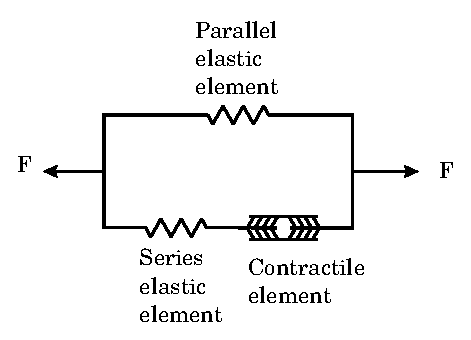
\includegraphics{chapters/introduction/figures/Hill_muscle_model}
\caption{The classical three-element Hill muscle model with one
  contractile element and two non-linear springs, one arranged in
  series and one parallel. }
\label{fig:hill_muscle_model}
\end{figure}



The \emph{active stress} approach is based on the classical three element
Hill model illustrated in Figure \ref{fig:hill_muscle_model}, where the
active contribution naturally decomposes the total stress into a sum
of passive and active stresses
\cite{nash2004electromechanical}. Hence, in the active stress
formulation \cite{hunter1998modelling} one assumes that the total
Cauchy stress $\Cauchy$ can be written as an additive sum of one
passive contribution $\Cauchy_p$ and one active contribution $\Cauchy_a$,
\begin{align}
  \Cauchy = \Cauchy_p + \Cauchy_a
\end{align}
The passive contribution is determined by the material model used
\begin{align}
 \Cauchy_p = \frac{1}{J} \frac{\partial \Psi(\F)}{\partial \F} \F^{T},
\end{align}
while the active contribution is given by 
\begin{align}
  \Cauchy_a = \Cauchy_{ff} \Fef \otimes \Fef +
  \Cauchy_{ss} \mathbf{s} \otimes \mathbf{s} +
  \Cauchy_{nn} \mathbf{n} \otimes \mathbf{n},
\end{align}
and the different constants $\Cauchy_{ff}, \Cauchy_{ss}$, and
$\Cauchy_{nn}$, which are the active stress in the fiber, sheet and
sheet-normal direction respectively, are typically coupled to the
electrophysiology and calcium dynamics.
There are experimental evidence that the active stresses in the
transverse direction of the fibers ($\Cauchy_{ss}$, and $\Cauchy_{nn}$),
are non-negligible \cite{lin1998multiaxial}, and one approach is to assume
a uniform transverse activation in which the total active tension
can be written as 
\begin{align}
  \Cauchy_a = T_a \left[\Fef \otimes \Fef +
   \eta\left( \mathbf{s} \otimes \mathbf{s} +
  \ \mathbf{n} \otimes \mathbf{n} \right)\right],
  \label{eq:intro_active_stress}
\end{align}
where $\eta$ represent the amount of transverse activation and $T_a
\in \mathbb{R}$ is the magnitude of the active tension.
In the limiting case ($\eta = 0.0$), the active tension acts purely
along the fibers and \eqref{eq:intro_active_stress} reduces to 
\begin{align}
  \Cauchy_a = T_a \Fef \otimes \Fef.
\end{align}
Note that, by observing  that
\begin{align*}
  \frac{\partial I_{4\mathbf{a}_0}}{\partial \F}
  = \frac{\partial (\mathbf{a}_0  \cdot \C \mathbf{a}_0 )}{\partial \F}
  = 2 \mathbf{a} \otimes \mathbf{a}_0 \implies
  \mathbf{a} \otimes  \mathbf{a}= \frac{1}{2} \frac{\partial I_{4\mathbf{a}_0}}{\partial \F} \F^{T}
\end{align*}
and that $I_1 =  I_{4\ef} +  I_{4\eS} +  I_{4\en}$, 
we can instead decompose the strain-energy function into a passive and active
parts \cite{pathmanathan2010cardiac}, $\Psi= \Psi_p + \Psi_a$, with
\begin{align}
\Psi_a = \frac{T_a}{2J} \left(( I_{4\ef} - 1)  + \eta \left[ (I_1 - 3) -
    (I_{4\ef} - 1)\right] \right), 
\end{align}
so that $J \Cauchy_a  = \frac{\partial \Psi_a}{\partial \F}
\F^{T}$.

The \emph{active strain} formulation is a relatively new way of modeling the
active contraction in the heart and was first introduced in
\cite{taber2000modeling}. This formulation is based on a
multiplicative decomposition of the deformation gradient, 
\begin{equation}
 \F = \F_e \F_a.
\label{eq:active_strain}
\end{equation}


The active part $\F_a$, is an inelastic process driven by the
biochemistry and can be seen as the actual distortion of the
microstructure. The elastic part $\F_e$ is responsible for preserving
compatibility of the tissue and stores all the energy in the
deformations. As a consequence, the strain energy function is a
function of the elastic deformation gradient only. The
decoupling can illustrated by considering two sarcomeres connected in
series as shown in Figure \ref{fig:actstrain}. 

\begin{figure}[htbp]
  \centering
    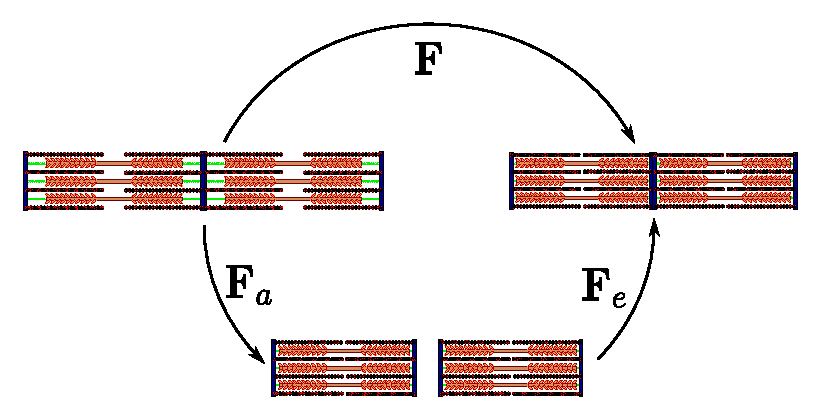
\includegraphics{chapters/introduction/figures/actstrain}
\caption{Illustration of the active strain formulation. During the active
deformation, the sarcomeres shortens as if they were all detached. The
elastic deformation ensures compatibility of the tissue.}
\label{fig:actstrain}
\end{figure}


The general form of the active deformation gradient for a
material with an orthotropic active response is given by
\begin{equation}
  \F_a =  \I
  - \gamma_f \ef \otimes \ef
  - \gamma_s \eS \otimes \eS
  - \gamma_n \en\otimes \en
 \label{eq:active_strain_Fa_general}
\end{equation}

We add the constraint $\det(\F_a) = 1$, meaning that the active
deformation is volume preserving. Further we assume that the activation is
transversely isotropic, so that the sheet and sheet-normal axis is
treated in the same way. It is then straight forward to verify that
$\gamma_n = \gamma_s =1- (1-\gamma_f)^{-1/2}$, and we have
\begin{equation}
  \F_a = (1 - \gamma) \ef \otimes \ef  + \frac{1}{\sqrt{1 - \gamma}} (\I - \ef \otimes \ef), 
 \label{eq:intro_active_strain_Fa_gjerald}
\end{equation}
where we set $\gamma = \gamma_f$ for convenience. 


While the motivation behind the active stress formulation is purely
physiological and based on the classical Hill model shown in Figure
\ref{fig:hill_muscle_model}, the motivation behind the active strain
formulation is more driven by ensuring mathematical robustness. In
particular it has been shown \cite{ambrosi2012active} that with the
active strain formulation, properties such as frame invariance and
rank-one ellipticity is inherited from the strain energy function. In
contrast, rank-one ellipticity is not guaranteed for the active stress
formulation.

For a more extensive comparison of the active stress and active strain
approach we refer to \cite{ambrosi2012active,giantesio2017comparison},
and for an overview of other methods to model the active contraction
we refer to \cite{goriely2017five}.



\subsection{Implementation details}
The cardiac mechanics solver developed during the work of this thesis
is implemented using the finite element framework FEniCS. Here we
briefly explain the main components of FEniCS as well as some
numerical considerations made when implementing the solver.


\subsubsection{The FEniCS Project}
\label{sec:fenics}

The FEniCS project is an open-source computing platform for solving
partial differential equations (PDEs) using the finite element method (FEM).
Solving PDEs using FEM involves many implementation details that can
be tedious to implement yourselves. The idea behind FEniCS is to
automate code generation so that the user can spend more time on doing
research and less time on implementation of assembly matrices. At the
core of FEniCS is DOLFIN \cite{logg2012dolfin}, which is C++/Python
library, and works as the main interface in FEniCS. In this thesis
only the Python interface has been used, in which C++ code is
automatically generated using SWIG. This allows for simplicity through
the Python scripting language and the speed of the C++ language.
The domain specific language used to represent weak formulations is
called the Unified Form Language (UFL) \cite{alnaes2014unified}, and
allows for e.g automatic differentiation of forms and expressions. The
FEniCS form compiler (FFC) \cite{logg2012ffc} compiles code written in
UFL to Unified Form-assembly Code (UFC) \cite{alnaes2012ufc} which are
optimized C++ code. The Python interface also makes use of the Instant
module which allows for just-in-time (JIT) compilation of C++
code. The compiled code is also stored in a cache so that compilation
of a form only happens once. Also, the relatively new UFL Analyser and
Compiler System (UFLACS) allows for fast compilation of complex forms
such as variational formulations that include the Holzapfel Ogden
material model \eqref{eq:holzapel_full}. 

For more information about FEniCS, the reader is referred to the
official web page (\url{https://fenicsproject.org}) or any of the
cited literature.

\subsubsection{Numerical considerations}
The solution of non-linear problems such as the one described here are
typically solved using methods like Newton's method. The convergence of
such methods depends on the initial guess, and if the
initial guess is too far from the true solution, the solver might diverge.
Moreover, if the initial guess is close to the true solution the
convergence rate is in general quadratic.

Let us consider a
typical numerical problem of inflating the ventricular geometry from a
stress-free configuration to end-diastole. This involves increasing
the pressure, or the boundary traction on the endocardium, from zero
to the end-diastolic pressure. A strategy know as the
\emph{incremental load} technique is usually a good approach. In this
strategy you select some incremental step-size (for instance $0.4$
kPa), and increase the pressure linearly until the target pressure is
reached. If the solver diverges you decrease the step-size (for
instance by a factor of 0.5) until convergence is reached, and
continue to step up the pressure with the new step-size. This is very
robust, but definitely a slow approach. Since many of the 
constitutive models for myocardium consist of an exponential
relationship between the stress and strain (so called Fung-type
relation), the amount of stress needed to displace a material will be
higher if the material is a state with high strain compared to a state
of low strain. Therefore, in the low strain state, the Newtons solver
might perform fewer iterations to reach convergence when the load is increased. As a
result, one could improve the incremental load technique by adapting
the step size if the number of newton iterations are below a certain
threshold (for instance $8$ iterations).

An even more clever strategy uses a technique from bifurcation and
chaos theory and is known as numerical continuation
\cite{allgower2003introduction}.  Suppose we want to
solve the non-linear problem $F(\uvec, \lambda)=0$ with state variable
$\uvec$ and parameter $\lambda$. For instance $\uvec$ could be the
displacement and $\lambda$ could be the endocardial pressure.
The idea behind numerical continuation is that given a solution pair
$(\uvec_0, \lambda_0)$ there exist (under conditions stated by the
implicit function theorem) a solution curve $\uvec(\lambda)$ such that
$F(\uvec(\lambda), \lambda)=0$ and $\uvec(\lambda_0) = \uvec_0$.
To explicitly find such a curve is not always easy but a simple
approximation can be found by extrapolation: Given two pairs
$(\uvec_0, \lambda_0)$ and $(\uvec_1, \lambda_1)$, and a new target
parameter $\lambda_2$, a possible solution is 
\begin{align}
  \uvec_2 =  (1-\delta)\uvec_0 + \delta \uvec_1 && \delta = \frac{\lambda_2 - \lambda_0}{\lambda_1 - \lambda_0}.
\end{align}
% Let $w_0$ denote the initial
% state variable associated with endocardial pressure $p_0$. Increase
% the pressure $p_1 = p_0 + \Delta p_0$, and solve to obtain $w_1$. Next
% we would like to solve for $p_2 = p_1 + \Delta p_1$ where $\Delta
% p_1$ might be the adapted step size. In stead of using $\tilde{w_2}=w_1$ as
% initial guess for the newton solver, as we typically would do in the incremental load
% technique, we observe that if $\delta = \frac{p_2 - p_0}{p_1 - p_0}$,
% and hence $p_2 = (1-\delta)p_0 + \delta p_1$, then a better choice
% of intial guess would be $\tilde{w_2} = (1-\delta)w_0 + \delta w_1$.
Choosing $\uvec_2$ as initial guess for the non-linear solver has been
successfully performed by others in non-linear cardiac mechanics
problems \cite{pezzuto2013mechanics}, and this approach is also used
in this thesis. 





%%% Local Variables:
%%% mode: latex
%%% TeX-master: "../../main"
%%% End:
\newpage
\section{Patient Specific Model Generation}

In this section we will describe 

\subsection{Geometry and microstructure}

The geometry of a patient's heart can be aquired using medical
imaging techniques, such as echocardiography (ultracound), magnetic
resonance imaging (MRI) or computed tomography (CT). Each modality off
advantages and disadvatages over the other. For example, MRI provides
high quality images, uses zero radiation, but is exspensive and lacks
temporal resolution. CT can more accuratley reconstruct the 3D image
in contrast to MRI, in which 2D slices needs to be glued together to
form a 3D surface. However, CT exposes the patient to radiation which
increases the chance of developing cancer. Finally echocardiography is
easy to use, cheap, harmless, and  has good temporal resolution, but
is clearly inferior when it comes to image quality.

The main modality used in this thesis is 3D echocardiography



\begin{itemize}
  \item Segmentation and aquisition using echopach
  \item From closed endo- and epicardial surfaces to a mesh
    (smoothing, cutting, orienting).
  \item Marking of mesh accoring to AHA segments (16,17,18)
  \item Local basis
  \item Rule based fibers
  \item Referece to mesh{\_}generation and patient repositories
\end{itemize}

\subsection{Continuum description of the heart}

\begin{itemize}
  \item Reference to mehcanics book
  \item Introduce basic notation (stress, strain, deformation)
\end{itemize}

We represent the heart as a continuum body  embedded in
$\mathbb{R}^3$. Let $\Xvec$ and  $\xvec$ denote the corresponding
coordinate in the reference and current configuration respectively.
The motion of a point $\Xvec$ in the reference configuration to the
point $\xvec$ in the current configuration  may be described by a
deformation map  $\varphi :  \mathcal{B}_0  \rightarrow \mathcal{B}$.
The deformation gradient associated with the motion $\xvec =
\varphi(\Xvec)$ is a rank-2 tensor given by  
\begin{align}
\F(\Xvec) = \frac{\partial \varphi}{\partial \Xvec}, 
\end{align}
The deformed and reference configuration are related via the
displacement field $\uvec$ by: 
\begin{align}  
\uvec = \xvec-\Xvec = \chi( \Xvec, t) -\Xvec,
\end{align} 
Further, we let $J = \det \F$ be the determinant of the deformation gradient 
and $\C = \F^T\F$ the right Cauchy-Green deformation tensor.\cite{holzapfel2000nonlinear}


\subsection{Passive behavior of the myocardium}

\begin{itemize}
  \item Hyperelasticiy, fung type-refer to relevant papers
  \item Incompressibility - Saddle point problem
  \item Finding the unloaded configuration
\end{itemize}



\subsection{Active behavior of the myocardium}


\begin{itemize}
  \item Active stress and strain (some mathematical aspects perhaps)
\end{itemize}




\subsection{Adjoint-based Data Assimilation}

\begin{itemize}
  \item Examples of data you want to constrain
  \item Forming of mismatch functional and problem formulation as
    PDE-constrained optimization.
  \item The adjoint approach. comparison with other methods.
  \item Control parameters
  \item Reference to pulse{\_}adjoint and pulse{\_}adjoint{\_}post
    repositories
\end{itemize}


We will now explain what we mean by ``adjoint-based'', and why this
approach is a key ingredient. The main theory presented here is taken
from the dolfin-adjoint web page. A word about dolfin adjoint...\ref{}
  
\begin{equation}
  \begin{aligned}
    \label{eq:opt_matparam}
    & \underset{m}{\text{minimize}}
    & &  I(\state, m) \\
    & \text{subject to}
    & & \delta \Pi(\state, \mvec) = 0, 
  \end{aligned}
\end{equation}

where $I(\state, m): \mathbb{W} \times \mathbb{Q} \mapsto
\mathbb{R}$ for some state space $\mathbb{W}$ and parameter space
$\mathbb{Q}$ and $\delta \Pi(\state) = 0$ is the force balance
equation given by \ref{}.


In order to apply optimisation algorithm...
We reduce the objective functional to be a function of the control
parameters only, $\hat{I}(\mvec) := I(\state(\mvec), \mvec)$. Consider an
initial value of the parmameters $\mvec = \mvec^0$. If $\hat{I}(m)$ is defined
and differentible in a neighborhood of $\mvec^0$ then $\hat{I}$ (and
consequently $I$) decreases fastest in the direction of the gradient, 
\begin{align}
  \nabla_{\mvec} \hat{I}(\mvec^0) = \begin{bmatrix}
    \frac{\mathrm{d} \hat{I}(\mvec^0) }{\mathrm{d} m_1},
    \frac{\mathrm{d} \hat{I}(\mvec^0) }{\mathrm{d} m_2},
    \cdots
    \frac{\mathrm{d} \hat{I}(\mvec^0) }{\mathrm{d} m_N}
  \end{bmatrix}^T.
  \label{eq:functional_gradient}
\end{align}
Here $\frac{\mathrm{d} \hat{I} }{\mathrm{d} m_i}$ represents the
total derivative:
\begin{align}
  \frac{\mathrm{d} \hat{I} }{\mathrm{d} m_i} = \frac{\mathrm{d} I (\state(\mvec), \mvec))}{\mathrm{d} m_i} = \frac{\partial  I }{\partial \state} \frac{\mathrm{d} \state}{\mathrm{d} m_i} + \frac{\partial  I }{\partial m_i}.
  \label{eq:functional_derivative_component}
\end{align}
In other words, the sequence
\begin{align}
  \mvec^{k+1} = \mvec^{k} - \gamma_k \nabla_{\mvec} \hat{I}(\mvec^k), \gamma_n \in \mathbb{R}
\end{align}
satisfies $\hat{I}(\mvec^{k+1}) \leq \hat{I}(\mvec^k) \; \forall k \geq
0$, and converges towards a local minimum. If $\hat{I}$ is convex then
the minimum is also global.
Being able to compute the gradient of the objective functional wrt to
the control parameters allows us to employ gradient based optimization
methods which are in general superior to gradient free methods.
One way to compute the gradient is by means of the finite difference
approach: For a given parameter $\mvec = \mvec^*$ we have
\begin{align}
  \frac{\mathrm{d} \hat{I} }{\mathrm{d} m_i}( \mvec^*) =
  \lim_{h \mapsto 0} \frac{\hat{I}(\mvec^* + h\mathbf{e}_i) - \hat{I}(\mvec^*)}{h}, 
\end{align}
where $\mathbf{e}_i \in \mathbb{Q}$ is the $i$'th canonical basis
vector. If $\dim(\mathbb{Q}) = N$, this approach would require $N+1$
functional evaluations. Moreover, since the state-variables depends upon the
control variables, we would also need to solve the force balance
equation $N+1$ times, which is typically very copmutationally
expensive. Hence, this approach is typically infeasable when the
dimesion of your parameterspace is large. In this case the adjoint
approach is much better. If $A$ is an operator (e.g a matrix), then
the adjoint operator $B$ satisfies the relation $\langle Au, v \rangle
= \langle u, Bv \rangle$, and we write $ B = A^*$. Here $(\cdot)^*$
denotes the Hermitian transpose, which in the case where $A$ is a real
matrix is just the transpose of $A$, $A^T$.  


Note that the gradient in
\eqref{eq:functional_gradient} can be rewritten (using the chain rule)
as
\begin{align}
  \nabla_{\mvec} \hat{I} =  \frac{\partial  I }{\partial \state} \nabla_{\mvec} \state
  + \frac{\partial  I }{\partial \mvec},
  \label{eq:functional_gradient_chain}
\end{align}
in which the $\dim(\mathbb{V}) \times \dim(\mathbb{Q})$ matrix
$\nabla_{\mvec} \state$ is difficult to compute.
Differentiating the force-balance equation \ref{} with respect to the
control parameters yields
\begin{align}
  & \nabla_{\mvec} \delta \Pi(\state, \mvec) = 0 \\
  \implies & \frac{\partial  \Pi }{\partial \state} \nabla_{\mvec} \state
  + \frac{\partial  \Pi }{\partial \mvec} = 0 \\
  \implies & \nabla_{\mvec} \state =
             - \left( \frac{\partial  \Pi }{\partial \state} \right)^{-1} \frac{\partial  \Pi }{\partial \mvec}.
\end{align}
Inserting this expression for $\nabla_{\mvec} \state$ into
\eqref{eq:functional_gradient_chain}, gives
\begin{align}
  \nabla_{\mvec} \hat{I} =  - \frac{\partial  I }{\partial \state}
  \left( \frac{\partial  \Pi }{\partial \state} \right)^{-1} \frac{\partial  \Pi }{\partial \mvec}
  + \frac{\partial  I }{\partial \mvec}.
\end{align}






%%% Local Variables:
%%% mode: latex
%%% TeX-master: "../../main"
%%% End:

\newpage

\section{Summary of papers}


\subsection{Paper 1}

\subsection{Paper 2}

\subsection{Paper 3}

\subsection{Paper 4}


\section{Other contributions}
Along with the research articles presented in this thesis, other
types of contributions in terms of talks, posters and software has
been made during the writing of this thesis. These contributions are
listed below.

\subsection{Talks}
\begin{itemize}
  \item Henrik Finsberg, Gabriel Balaban, Joakim Sundnes, Hans
    Henrik Odland, Marie Rognes, and Samuel T. Wall. ``Patient
    Constrained Ventricular Stress Mapping'',
    Conference Presentation at MALT 2015,  Lugano, Switzerland (2015).
  \item Henrik Finsberg, Gabriel Balaban, Joakim Sundnes, Marie
    Rognes, and Samuel T. Wall. ``Personalization of a Cardiac
    Compuational Model using Clinical Measurements'', Conference
    Presentation at 28th Nordic Seminar on Computational
    Mechanics. Vol. 28. Tallin, Estonia, (2015).
  \item Henrik Finsberg, Gabriel Balaban, Joakim Sundnes, Marie
    Rognes, and Samuel T. Wall. ``Optimization of a Spatially Varying
    Cardiac Contraction parameter using the Adjoint Method'',
    Conference Presentation at FEniCS 16, Oslo, Norway,(2016).
  \item Finsberg, Henrik N., Gabriel Balaban, Joakim Sundnes, Hans
    Henrik Odland, Marie Rognes, and Samuel T. Wall. ``Personalized
    Cardiac Mechanical Model using a High Resolution Contraction Field
    '',  Conference Presentation at VPH16 Translating VPH to the
    Clinic,  Amsterdam, Netherlands (2016).
\end{itemize}


\subsection{Posters}
\begin{itemize}
  \item Henrik Finsberg, Gabriel Balaban, Joakim Sundnes, Marie
    Rognes, and Samuel T. Wall. ``Patient Specific Modeling of Cardiac
    Mechanics using the Active Strain Formulation '',
    Geilo Winter School, Geilo, Norway, (2016).
  \item Henrik Finsberg, Ce Xi, J. Tan, L. Zhong, LC Lee, Joakim
    Sundnes, and Samuel T. Wall. ``Mechanical Analysis of Pulmonary
    Hypertension via Adjoint based Data Assimilation of a Finite
    Element Model '', Summer Biomechanics, Bioengineering, and
    Biotransport Conference, Tucson, AZ, (2017). 
  \end{itemize}


\subsection{Software}
  \urlstyle{rm}
\begin{itemize}
  \item Pulse-Adjoint, FEniCS-based cardiac mechanics solver and data
    assimilator, source: \url{https://bitbucket.org/finsberg/pulse_adjoint}
  \item Mesh-Toolbox, Toolbox for generating FEniCS meshes from 4D
    Echo,  source: \url{https://bitbucket.org/finsberg/mesh_generation}
\end{itemize}



\section{Closing remarks and future directions}

A couple remarks regarding the limitations of the methods used in this
thesis shoud be made. Here we start by listing a couple of statements
which should be taken into considerations. 


\begin{itemize}
\item \emph{The quality of features/biomarkers you can extract from a data-driven
model cannot be any better than the data used as input to the
model}. Most of the results presented in this thesis are based on data
obtained from clinical measurements of real patients.
\item \emph{The spatial resolution of the parameters should be
    reflected in the spatial resolution of the observations.} When
  trying to fit data that are spatially resolved at some level,
  choosing parameters that are resolved at a finer level should be
  done with caution. The continuity in the underlying physics as well
  as regularization techniques could be used to ...

\end{itemize}

During the work of this thesis, several questions still remains open
and would require

\begin{itemize}
\item The active model for the myocardium is has .. Degree of
  tranverse activation. Matching of strain data..
\item Identifiability of parameters... Uniqueness of
  solutions.. Amount of regularization.. Convexity of the mismatch functional
\item Appropriate boundary conditions.. In paper three we saw big
  differences in the choice of boundary conditions. Especially, the
  magnitude of the stress seems to 
\item Coupling of electrophysiologigy and mechanics in an
  ajoint-based. data assimilation framework. 
\end{itemize}

%%% Local Variables:
%%% mode: latex
%%% TeX-master: "../../main"
%%% End:



\newpage


\bibliographystyle{plain}
\bibliography{chapters/introduction/bibliography}


%%% Local Variables:
%%% mode: latex
%%% TeX-master: "../main"
%%% End:




\cleardoublepage


\graphicspath{{chapters/paper1/figures/}}


\chapter{Paper 1: \\High Resolution Data Assimilation of Cardiac
  Mechanics}

% \pagebreak
\clearpage

\renewcommand{\thefootnote}{\fnsymbol{footnote}}

\section*{High Resolution Data Assimilation of Cardiac Mechanics}

% \begin{center}
G. Balaban\footnotemark,
H. Finsberg\footnotemark[\value{footnote}], 
H. Odland, M. E. Rognes, \\
S. Ross, J. Sundnes, and
S. Wall
% \end{center}

\subsection*{Abstract}


% \clearpage
% \begin{abstract}

Computational models of cardiac mechanics, personalized to a patient, offer access 
to mechanical information above and beyond direct medical imaging.
Additionally, such models
can be used to optimize and plan therapies in-silico, thereby reducing risks and
improving patient outcome. Model personalization has traditionally been achieved by data
assimilation, which is the tuning or optimization of model parameters
to match patient observations.
Current data assimilation procedures for cardiac mechanics are limited in their ability
to efficiently handle high dimensional parameters.
This restricts parameter spatial resolution, and thereby the ability
of a personalized model to account for heterogeneities that are often present in
a diseased or injured heart.
In this paper we address this limitation by
proposing an adjoint-gradient based data assimilation method
that can efficiently handle high-dimensional
parameters. We test this procedure on a synthetic data set,
and provide a clinical example with
a dyssynchronous left ventricle with highly irregular motion.
Our results show that the method efficiently handles a high dimensional
optimization parameter, and produces an excellent agreement
for personalized models to both synthetic and clinical data.

% \end{abstract}
\footnotetext{Both of these authors contributed equally to this work.}
% \maketitle

\clearpage
\section{Introduction}
Computational models of cardiac mechanics, personalized to the level of the individual 
through the use of clinical imaging, have potential to be a powerful aid in the diagnosis and 
treatment of cardiac disease.  By relating image-based data to fundamental physical 
processes, models can give additional insight into the function or dysfunction of the 
individual's heart, beyond what can be directly measured or observed in the images. 
This is becoming more important as the resolution and accuracy of clinical imaging continues to 
improve.  This increasingly detailed data combined with biophysical models has promise 
in analysis of regionally and temporally resolved differences in the mechanics of the heart, 
important in diseases such as heart failure and the application of cardiac resynchronization therapy. 

A key step in making these clinically useful cardiac mechanics models is proper data assimilation from patient observations into a fit model. This involves the optimization, or tuning, of individual model parameters in order to make the model match the observations of the patient's heart.  Over the last decade several data assimilation methods have been developed and proposed for this problem. The earliest studies employed gradient based optimization in order to minimize the discrepancy between model-derived data and clinical observations.  The gradients necessary for these optimizations were calculated using direct differentiation \cite{sermesant2006cardiac}
or finite difference \cite{augenstein2005method, gao2015parameter, Wang2009}.
More recent efforts include the use of global optimization methods:
in particular genetic algorithms \cite{mojsejenko2014estimating,
sun2009computationally}, a Monte Carlo method \cite{neumann2014robust},
subplex algorithm \cite{wong2015velocity}, and parameter sweeps \cite{asner2015estimation, hadjicharalambous2015analysis}.
Finally, reduced order unscented Kalman filtering has also been successfully applied as
a data assimilation tool for patient-specific model creation \cite{chabiniok2012estimation,
xi2011myocardial, Marchesseau2013}.

The increasingly large amount of easily obtainable geometric and motion data, 
however, is a challenge for data assimilation into personalized computational models 
using the techniques mentioned above.  This is as the computational 
expense scales badly with the number of model parameters to be fit. In the 
case of the Kalman filtering strategies, at least one extra evaluation 
of the model is required per additional model parameter to be optimized.
The calculation of model-data mismatch gradients by finite difference 
or direct differentiation suffers from the same limitation. Global methods 
on the other hand are affected by the curse of dimensionality; that is, 
a rapid expansion of the space of parameters that must be searched as the number 
of dimensions increases. For high dimensional problems 
the run-time needed to carry out a global search can be computationally prohibitive.

In contrast, the calculation of a functional gradient by the adjoint formula is 
nearly independent of the number of optimization parameters, requiring one forward and one backward 
adjoint solve of the mathematical model. The forward solve is typically needed to evaluate the functional, 
and the evaluation of the gradient at the same point requires only an additional backward solve of the adjoint system.
Furthermore, this backward solve is always linear, 
and therefore computationally less expensive than the forward solve 
if the mathematical model is nonlinear. These methods have been widely explored in model optimization, 
with adjoint-based data assimilation techniques having previously been
employed for cardiac mechanics, specifically using linear elastic models and
clinical data~\cite{Delingette2012, sundar2009biomechanically}, and
also nonlinears model combined with experimental
data~\cite{balaban2016adjoint}.

In this work we provide an improved data assimilation pipeline for high resolution optimization,
demonstrating the parameterization of mechanical contraction in high spatial resolution 
driven by 4D echocardiography patient data. This high dimensional optimization problem 
is efficiently solved using an adjoint gradient based technique, described in detail 
in our previous work \cite{balaban2016adjoint}. We demonstrate our method on the pathological 
case of a dyssynchronous left ventricle, which has complex and irregular motion, 
as well as on a synthetic case consisting of data generated by our mechanical model. 
This study is to the best of our knowledge the first to use adjoint-based data assimilation 
for nonlinear cardiac mechanics with clinical data, and the first to consider the 
resolution of a parameter at the same scale as the discretization of the cardiac geometry.
These are important considerations as better understanding of myocardial properties 
emerges and the collection of high resolution clinical data continues to expand.

The rest of this paper is organized as follows: In
Section~\ref{sec:methods} we present a mathematical model that
accounts for the three main drivers of ventricular mechanics; blood
pressure, tissue elasticity and muscle contraction.  
We also describe clinical measurements of a patient suffering from dyssynchrony, and our data assimilation procedure
for fitting the model to these measurements.
Numerical results are presented in Section~\ref{sec:num_results}, and discussed in
Section~\ref{sec:discussion}. Finally, we provide some concluding
remarks in Section~\ref{sec:conclusion}.


\section{Materials and Methods}
\label{sec:methods}

\subsection{Wall motion modelling}

\label{sec:wall_motion}
In order to estimate the position of the myocardial walls through
the cardiac cycle we adopt a continuum mechanics description of
cardiac wall motion. In this description we consider a fixed left
ventricular reference geometry $\Omega$, with endocardial boundary
$\lvendo$, and basal boundary $\basebound$.

Our fundamental quantity of interest is the vector valued displacement
map $\uvec(\mathbf{X})$, where $\mathbf{X} \in \Omega$.  At any given
point in time in the cardiac cycle, $\uvec(\mathbf{X})$ relates
the current geometry $\omega$ to the reference geometry by
 \begin{equation}
{\bf X} + {\bf u}({\bf X}) = {\bf x}, \quad {\bf x} \in \omega, \quad {\bf X} \in \Omega. 
\end{equation}

Assuming that the cardiac walls are in equilibrium,
it is possible to determine the value of $\uvec$ from the principle of
virtual work
\begin{equation}
  \label{eq:work-balance}
  \delta W(\uvec) = 0,
\end{equation}
which states that the virtual work, $\delta W(\uvec)$, of all forces
applied to a mechanical system vanishes in equilibrium. For our ventricular wall motion
model, the virtual work $\delta W(\uvec)$, is given by
\begin{equation}
\begin{aligned}
\label{eq:workdef}
 \delta W(\uvec, p) &= \int_{\Omega} \FPK : \Grad \ \du \ dV 
		  + \int_{\Omega} (J - 1) \dpre + p J \F^{-T} : \Grad \ \du \ dV  \\
		 &+ \plv \int_{\lvendo} J \F^{-T} \Nvec \cdotp \du \ dS 
		  +  \int_{\lvbase}  k \uvec \cdotp \du \ dS.
 \end{aligned}
\end{equation}
Here we have introduced the hydrostatic pressure $p$ in order to enforce the 
incompressibility constraint $J =1$, with $J = \det \F = \det  \left(\Grad \ \uvec + \mathbf{I}\right)$, 
and $\mathbf{I}$ being the second order identity tensor. 
Furthermore, $\Nvec$ denotes the unit outward normal vector, $k$ 
the constant of a spring that we introduce at the basal boundary, and $\plv$ the intra-ventricular 
blood pressure. The virtual variables $\du$ and $\dpre$ are test functions whose values
are arbitrary when the system \eqref{eq:work-balance} is in mechanical
equilibrium.

In order to anchor the computational geometry, we fix $\uvec$ in the longitudinal direction 
at the base by using a Dirichlet boundary condition. At the epicardial boundary normal
forces are set to 0, and so there is no term for this boundary in
\eqref{eq:workdef}.

The internal stresses of our model are given by $\FPK$, the first Piola-Kirchhoff tensor,
which can be calculated as a derivative of a strain energy functional
in the case of a hyperelastic material.
In our model we employ a reduced version~\cite{Krishnamurthy2013, gjerald2015patient,
  asner2015estimation, hadjicharalambous2015analysis} of the
Holzapfel-Ogden strain energy law~\cite{Holzapfel2009}, 
\begin{equation}
\label{eq:hoa}
 \psi(\C) = \frac{a}{2 b} \left( e^{ b (I_1(\C)
 - 3)}  -1 \right)
 + \frac{a_f}{2b_f} \left( e^{ b_f (I_{4f}(\C)
 - 1)_+^2} -1 \right),
\end{equation}
which gives the amount of strain energy, $\psi$, stored per unit
volume myocardium undergoing the strain $\C = \F^{T} \F$.
The notation
$(\cdotp)_{+}$ refers here to $\max\{\cdotp, 0\}$.  Furthermore
the mechanical invariants $I_1$ and $I_{4f}$ are defined as
\begin{equation}
I_1(\C) = \tr \C,  \quad \quad I_{4f} = \ef \cdotp \C \ef,
\end{equation}
with $\ef$ indicating the local myocardial fiber direction. The
material parameters $a, a_f, b, b_f$ are scalar quantities which influence the shape of
the stress-strain relationship, and can be adapted to personalize the
elastic properties of a myocardial tissue model to a specific patient.

The Lagrange multiplier formulation of incompressibility that we 
 employ enforces its constraint only weakly. This can cause
 convergence issues in the numerical solution of the work balance equation~\eqref{eq:work-balance}. We therefore
 eliminate volumetric strains from the energy function \eqref{eq:hoa}
 by a simple modification
 \begin{equation}
  \tilde{\psi}(\C) = \psi(J^{-\frac{2}{3}}\C).
 \label{eq:strain_energy}
 \end{equation}
 This modification has been shown to improve the robustness of
 Newton-Raphson methods applied to incompressible hyperelastic
 problems~[Figure 3C of \cite{land2015improving}].

In order to account for muscle contraction we apply the 
active strain framework~\cite{nardinocchi2007active}.  In this framework the amount
of muscle fiber shortening is specified by a field $\gamma$ via
a split of the deformation gradient
\begin{equation}
  \label{eq:fsplit}
  \F = \F_e \F_a(\gamma),
\end{equation}
where $\F_e$ is the elastic part and $\F_a(\gamma)$ the active
part of the deformation gradient. For the value of $\F_a(\gamma)$
we adopt a simple relation~\cite{gjerald2015patient, evangelista2011torsion} which satisfies
the incompressibility constraint by design and directly relates the
amount of active fiber shortening to the value of $\gamma$
\begin{equation}
  \F_a = (1 - \gamma) \ef \otimes \ef  + \frac{1}{\sqrt{1 - \gamma}} (\I- \ef \otimes \ef).
 \label{eq:active_strain}
\end{equation}
In the case $\gamma = 0$ there is no muscle shortening at all, and the
amount of shortening increases with increased $\gamma$ up to the
theoretical limit of $\gamma = 1$. Physiologically, $\gamma$ models the 
length change along muscle fibers neglecting elastic effects. This, together with the elastic
resistance gives the strength of the muscle contraction.

Muscle contraction is accounted for in terms of virtual work by
modifying the first Piola-Kirchhoff stress tensor, so
that the strain energy only depends on the elastic part of the
deformation
\begin{equation}
 \FPK = \frac{\partial \tilde{\psi}}{\partial \F} = \frac{\partial \tilde{\psi} (\C_e)}{\partial \F}
\label{eq:active_strain_energy}
\end{equation}
with $\C_e = \F_e^T\F_e$.

Given an amount of fiber shortening $\gamma$, the value of the elastic
 parameters $a, b, a_f, b_f$, the intraventricular blood pressure
 $\plv$ and the spring constant $k$, the myocardial wall displacement
 $\uvec$ and hydrostatic pressure $p$ can be obtained by solving the
 principle of virtual work \eqref{eq:work-balance}. 

 \subsection{Clinical measurements}
\label{sec:clinical_measurements}
Clinical data were obtained at the Oslo
University Hospital in the context of the Impact study \cite{ImpactStudy2016}. Specifically,
we consider the case of an 82 year old man in NYHA functional 
class III systolic heart failure with coronary
artery disease, and left bundle branch block.
A left bundle branch block normally causes both electrical and mechanical 
dyssynchrony. In this case the ECG revealed a
QRS width of 140 ms and the echocardiographically derived ejection fraction of 30 \%.

Prior to cardiac resynchronization therapy implant,
the patient had echocardiographic and left ventricular (LV)
pressure measurements taken, which are the basis for the clinical
data used in this study. Pressure recordings were carried out
with an intravascular pressure sensor catheter
(Millar micro catheter) that was positioned in the LV
via the right femoral artery. Pressure data were
obtained automatically and digitized (Powerlab system, AD Instruments) 
before offline analyses were performed with a low pass filter of 10Hz.

Images of the patient's left ventricle (LV) were captured with 4D
echocardiography using a GE Vingmed E9 machine (GE healthcare Vingmed, Honrten, Norway).
Speckle tracking motion analysis was carried out with GE's software package
EchoPac. Data from 6 beats were combined in EchoPac in order 
to obtain a single sequence of images for a single heartbeat. Analysis 
of these images resulted in LV cavity volume measurements as well as
regional strain curves defined for a 17 segment delineation of the LV
according to the AHA representation \cite{cerqueira2002standardized}.
The strain curves were measured in
the local left ventricular longitudinal, radial and circumferential
directions. Both strains and volumes were measured 34 times throughout the
cardiac cycle.

Valvular events were used to synchronize the pressure to the strain and
volume data. The timing of the observed valvular events in the images
were matched with the observed valvular events in the pressure
trace. In the pressure trace, aortic valve opening (AVO) was selected after the
steepest increase of the pressure ($\frac{dp}{dt}$ max ), and mitral valve
closure just before $\frac{dp}{dt}$ max . Aortic
valve closure (AVC) was chosen just before the pressure had its largest
decrease after AVO, and the mitral valve opening
before the pressure dropped down to baseline after AVC. 
A pressure-volume loop based on the synchronization is displayed in
Figure~\ref{fig:pv_loop_phases}.

Finally a linear correction of the strain curves was performed in order to 
eliminate drift; with drift being defined as the value of the strain obtained at
the end of the cardiac cycle. Theoretically drift should be zero for a stable cyclical heartbeat.
The linear correction enforces the cyclical property.

\subsection{Ventricular geometry generation}
\label{sec:compgeo}
The computational mechanics framework used for our wall motion model,
described in Section~\ref{sec:wall_motion}, requires a reference stress-free geometry from
which to define displacements. Such a geometry typically does not exist in-vivo due to the 
presence of blood pressure on the endocardial walls. Algorithms exist for calculating
stress free geometries given a loaded state \cite{bols2013computational, gee2010computational}.
However for the sake of simplicity we derive our reference geometry from an echocardiographic
image of the LV at the beginning of atrial systole,
as the pressure is near minimal at this point, and the ventricular myocardium
can be assumed to be relaxed.

From the image at the beginning of atrial systole, triangulated data points
for left ventricular endocardial and epicardial surfaces, along with a 17 segment delineation,
were extracted using the EchoPac software package.
The segment delineation was given on a so called strain mesh, which is a 2-D surface constructed by
EchoPac and located approximately in the mid wall of the LV.


We constructed a flat ventricular base by cutting the raw geometry
with a plane that was fit via least-squares to the points at the base.
After the fitting, the longitudinal position of the cutting plane was
adjusted so that the cavity volume of the resulting mesh agreed with
the measured volume to a tolerance of $1$ ml. Points on the epicardial
and endocardial surfaces that lay above the cutting plane were removed. 

We employed Gmsh \cite{geuzaine2009gmsh} to create a 
linear tetrahedral volumetric mesh between the endocardial and epicardial surfaces. 
This mesh had 1262 elements, and is shown in Figure~\ref{fig:compgeo_mesh}.
Myocardial fiber orientations were assigned using a rule based method,
with a fiber helix angle of $40$ degrees on the 
endocardium rotated clockwise throughout the ventricular wall 
to $-50$ degrees on the epicardium \cite{bayer2012novel}. 
A streamline representation of the local myocardial fibers is displayed
in Figure \ref{fig:compgeo_fibers}.

Finally, the AHA-segments from the strain mesh were transferred onto the volumetric mesh.
This was accomplished by computing prolate spherical coordinates for
the barycenter of each tetrahedron,
and then assigning an AHA-zone to the tetrahedron 
based on the corresponding prolate spherical coordinate in the strain mesh. 
AHA-segments on the volumetric mesh are shown in Figure~\ref{fig:compgeo_regions}.

\begin{figure}[htbp]
\centering
\begin{subfigure}[t]{0.25\textwidth}
     \centering
     \raisebox{2mm}{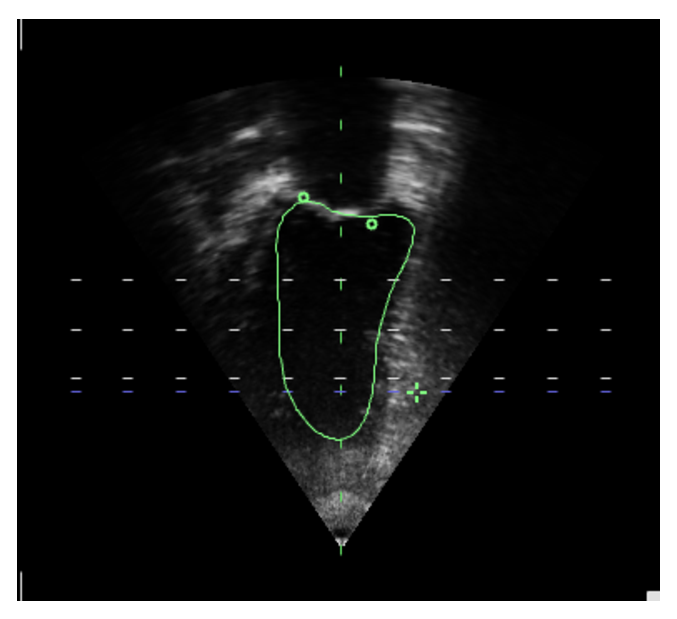
\includegraphics[width=0.9\textwidth]{LV_systole_volume_trace}}
     \caption{\label{fig:ultrasound_image}}
\end{subfigure}
\qquad
\begin{subfigure}[t]{0.25\textwidth}
    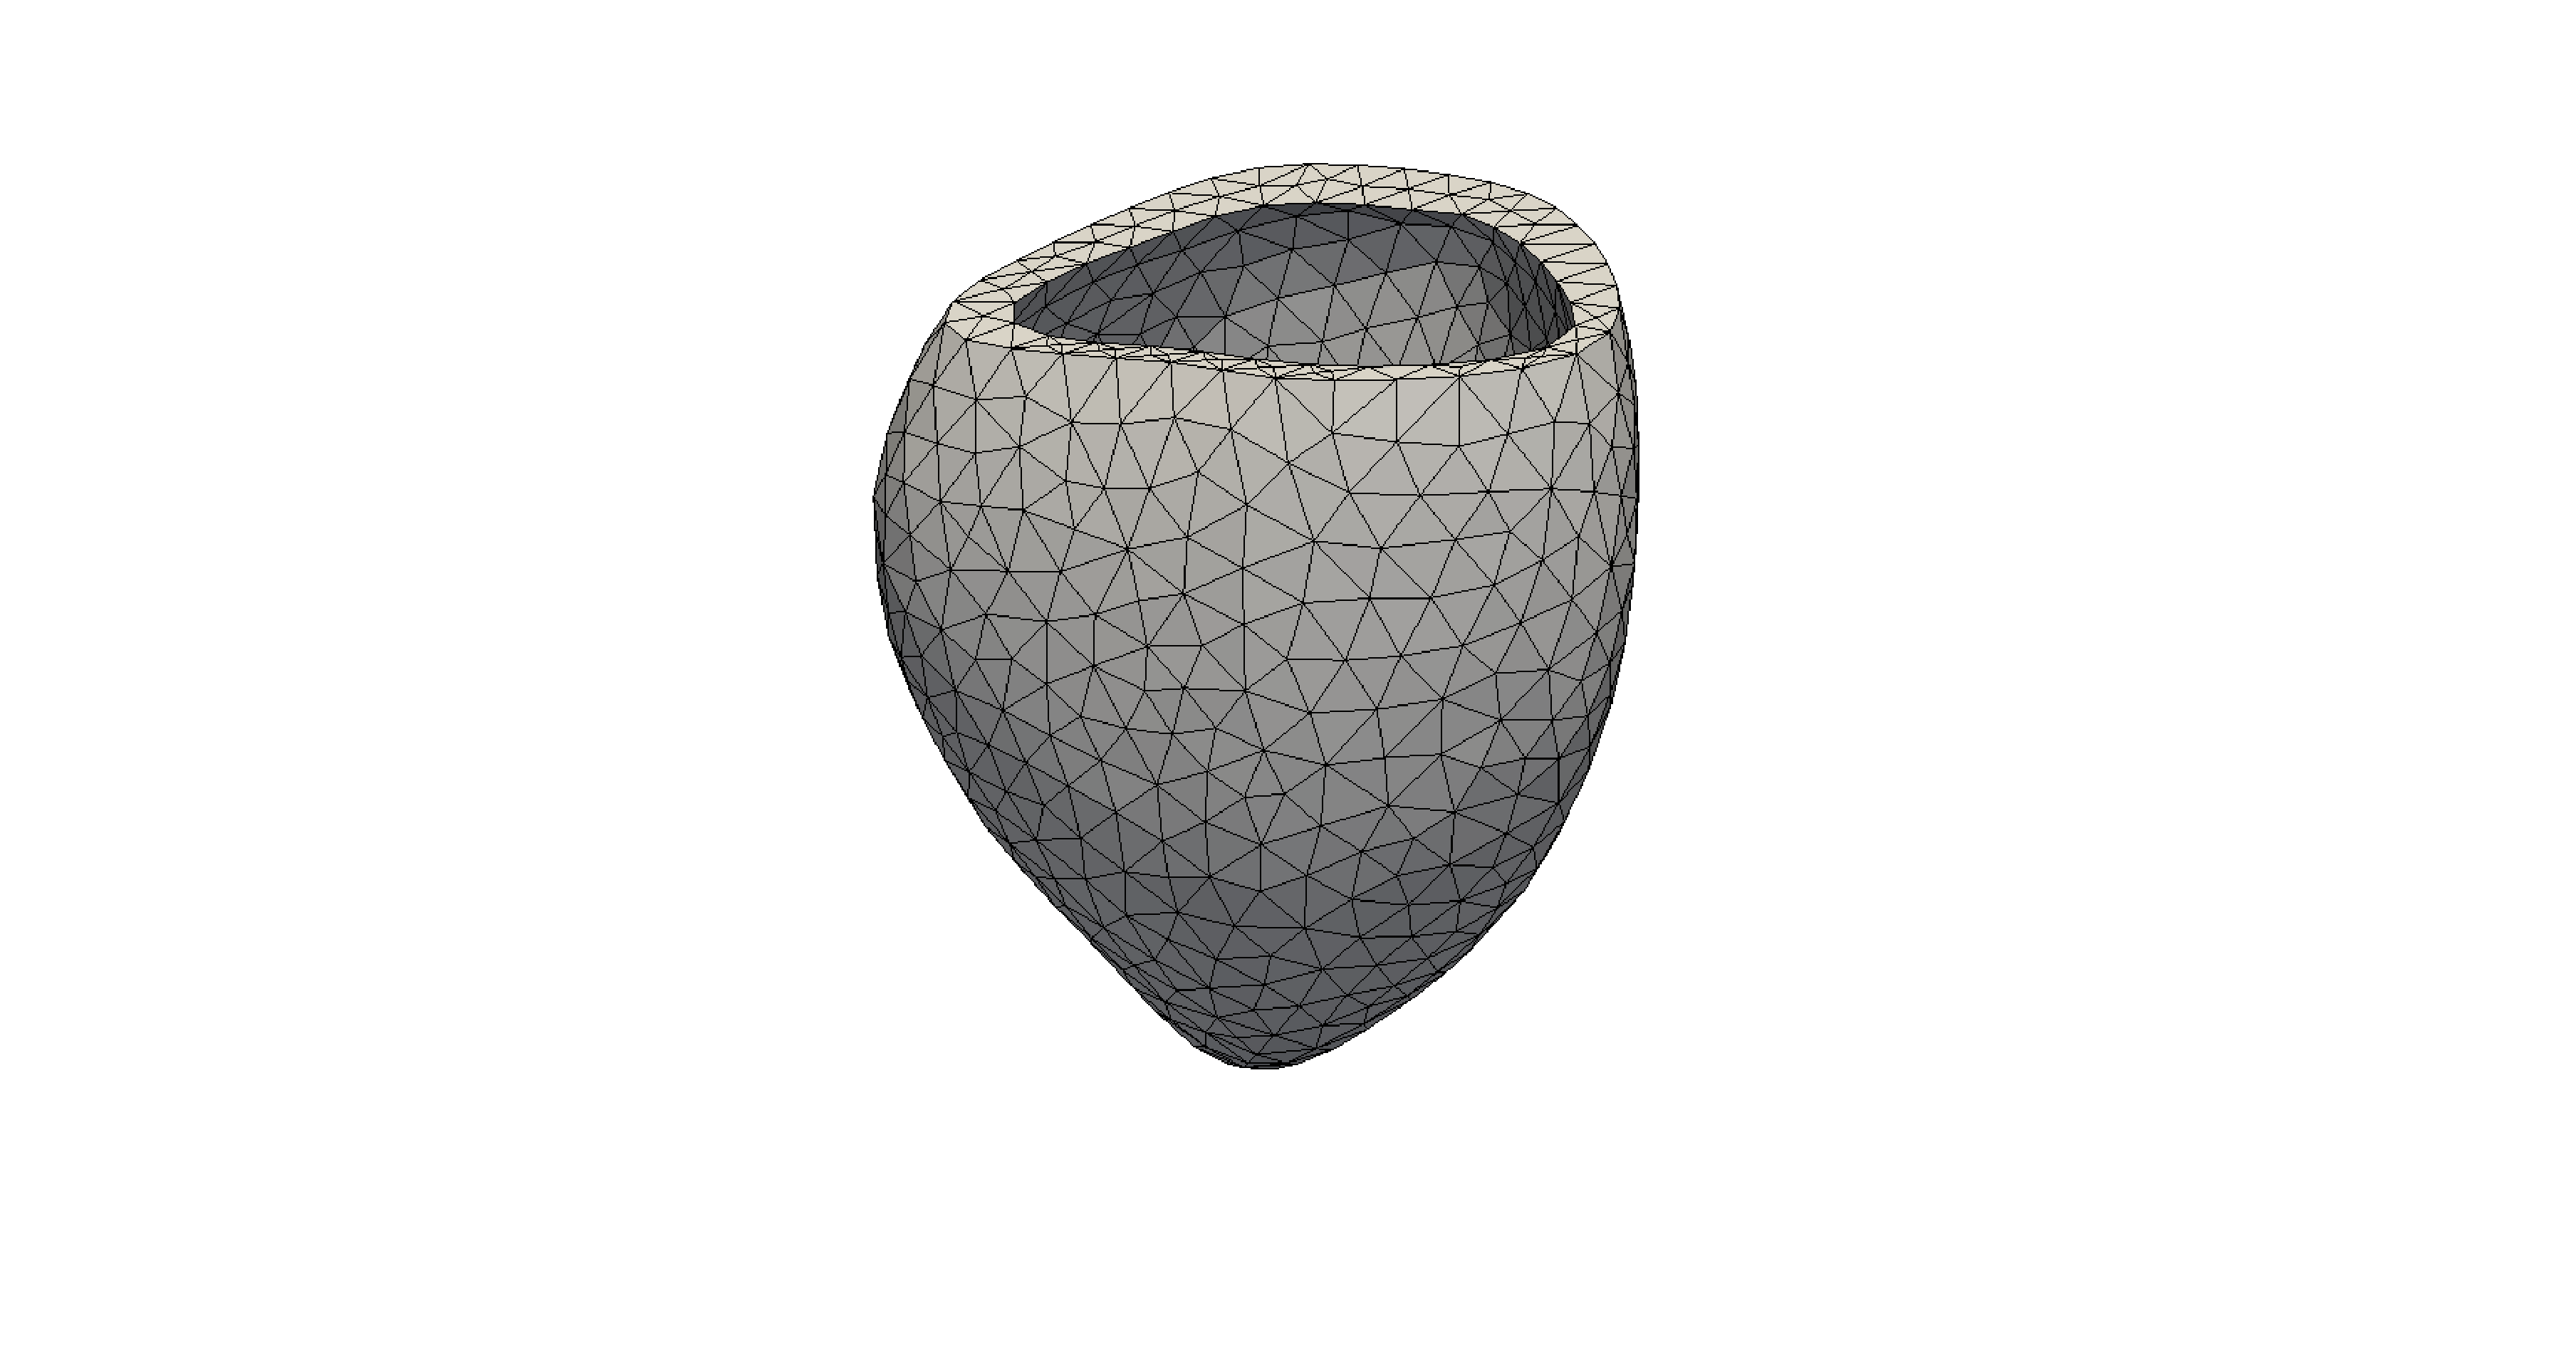
\includegraphics[width=\textwidth, trim={15cm 4cm 21cm 3cm}, clip]{mesh}
    \caption{\label{fig:compgeo_mesh}}    
\end{subfigure}
\qquad
\begin{subfigure}[t]{0.25\textwidth}
    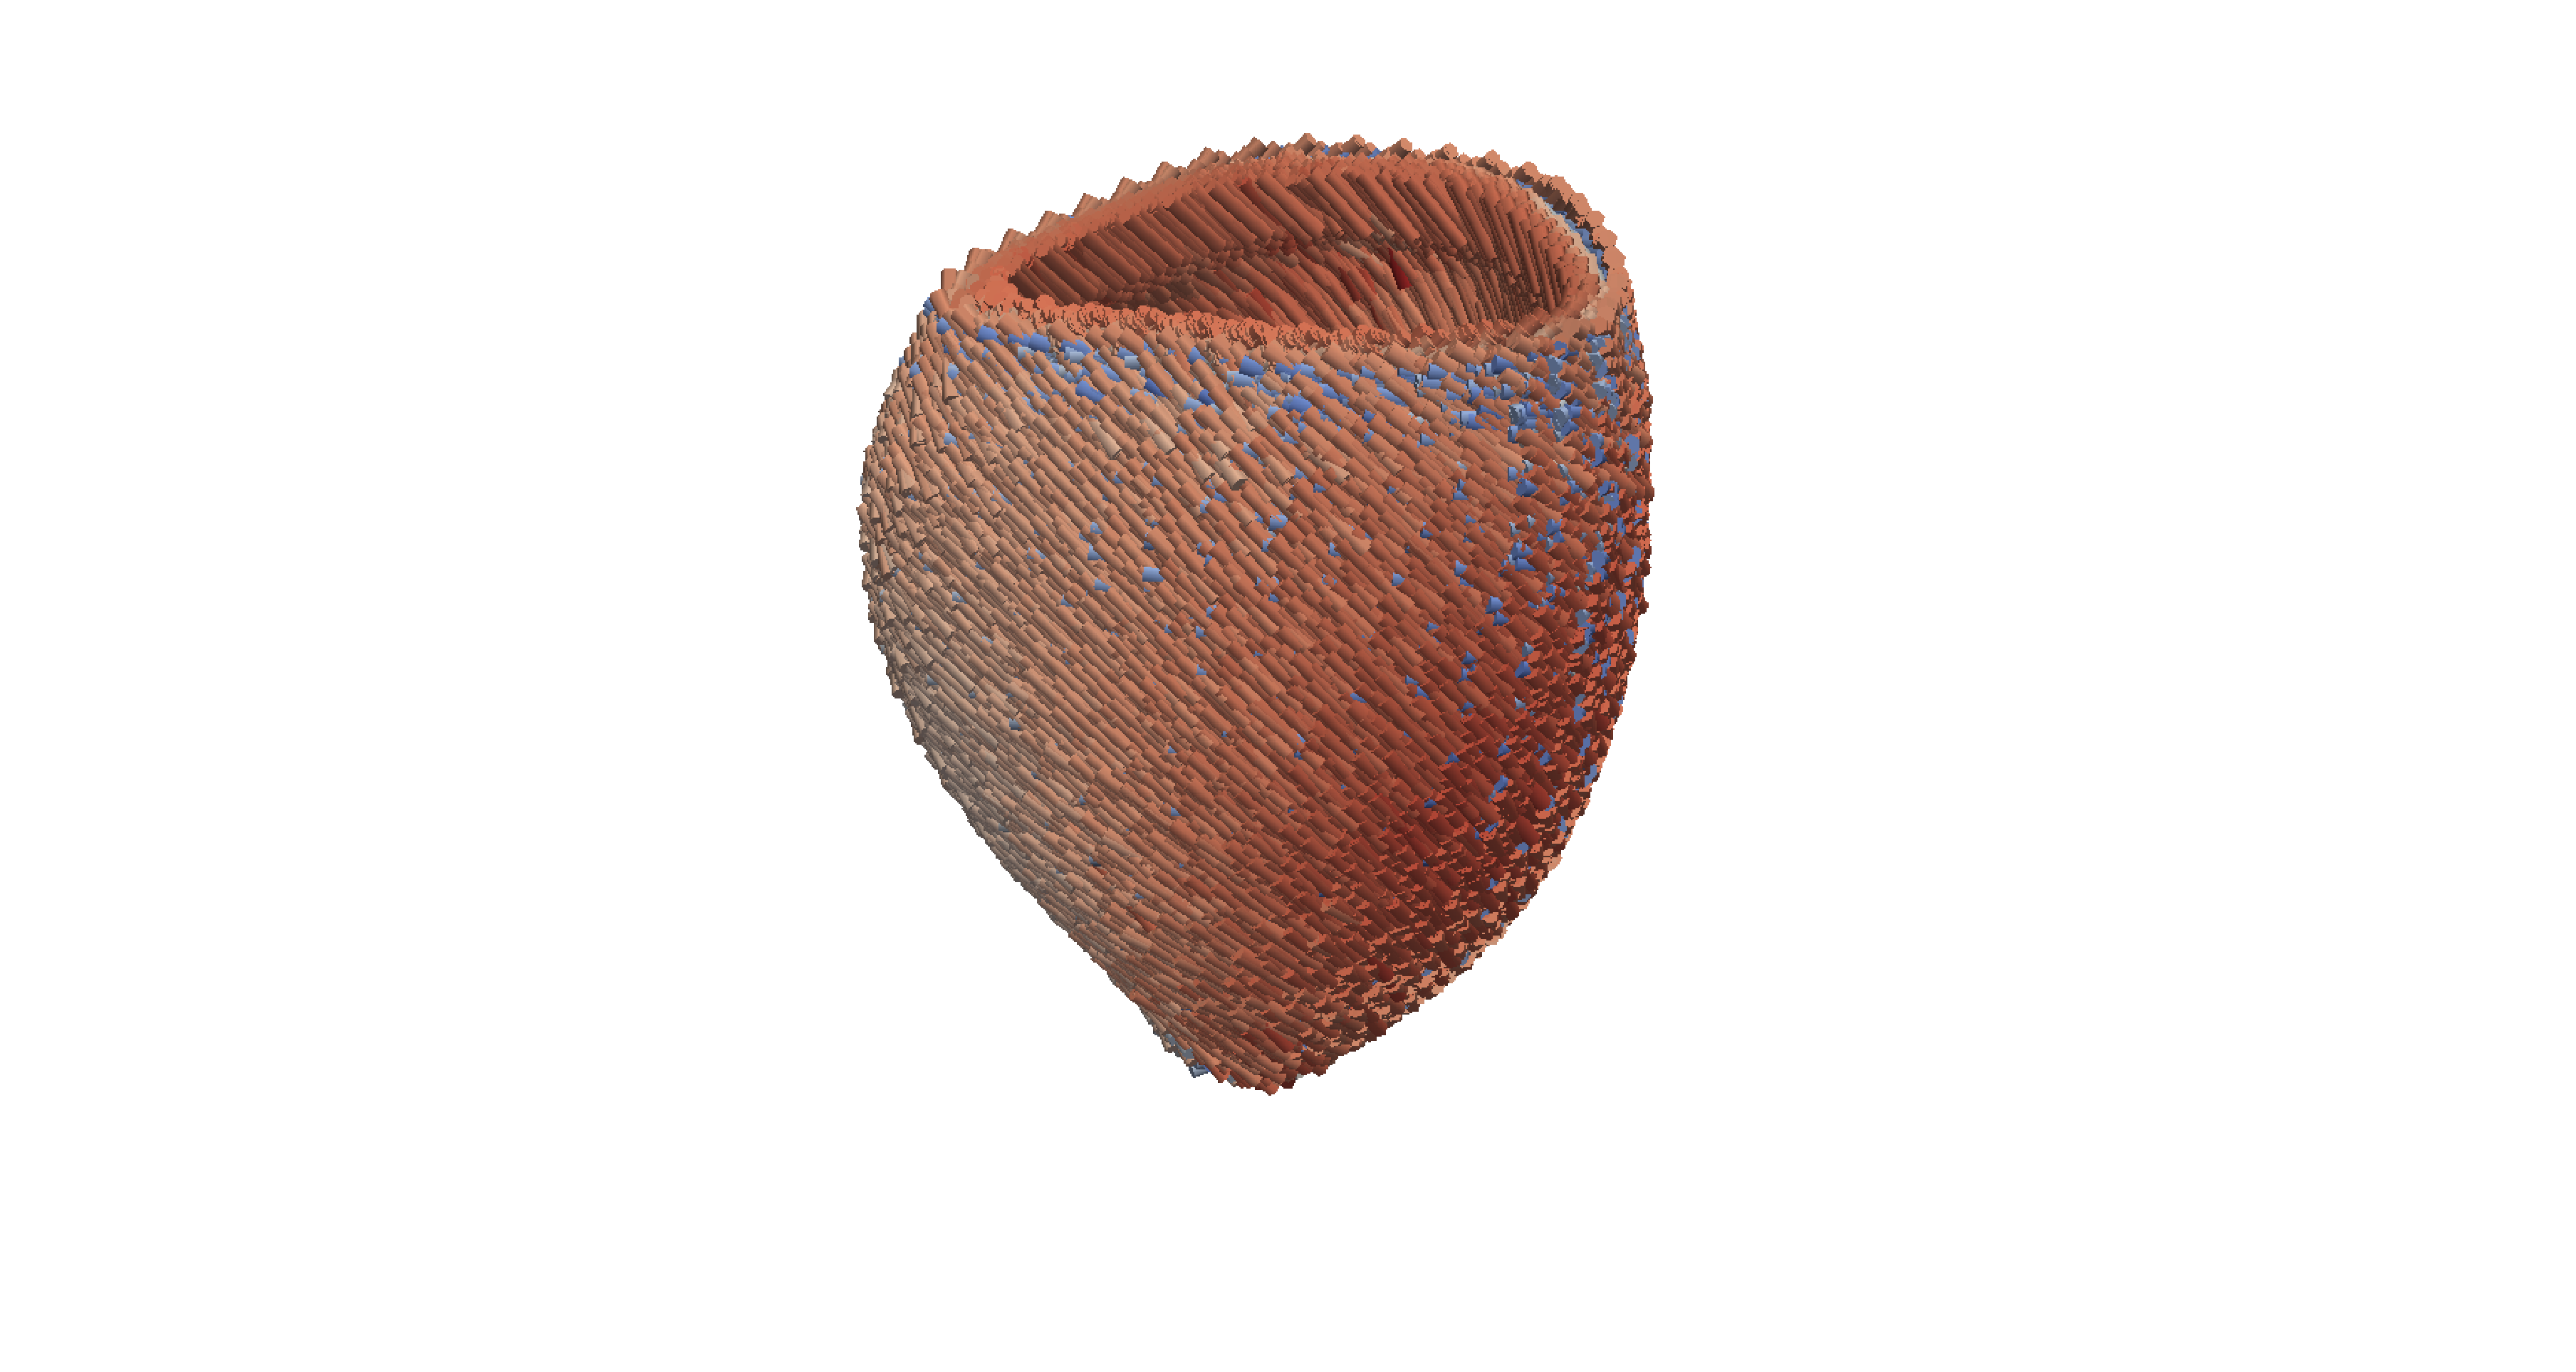
\includegraphics[width=\textwidth, trim={15cm 4cm 21cm 3cm}, clip]{fibers}
    \caption{\label{fig:compgeo_fibers}}
\end{subfigure}
\qquad
\begin{subfigure}[t]{0.25\textwidth}
    
\includegraphics[width=\textwidth, trim={15cm 4cm 21cm 3cm}, clip]{sfun}
    \caption{\label{fig:compgeo_regions}}
\end{subfigure}
\begin{subfigure}[t]{0.35\textwidth}
    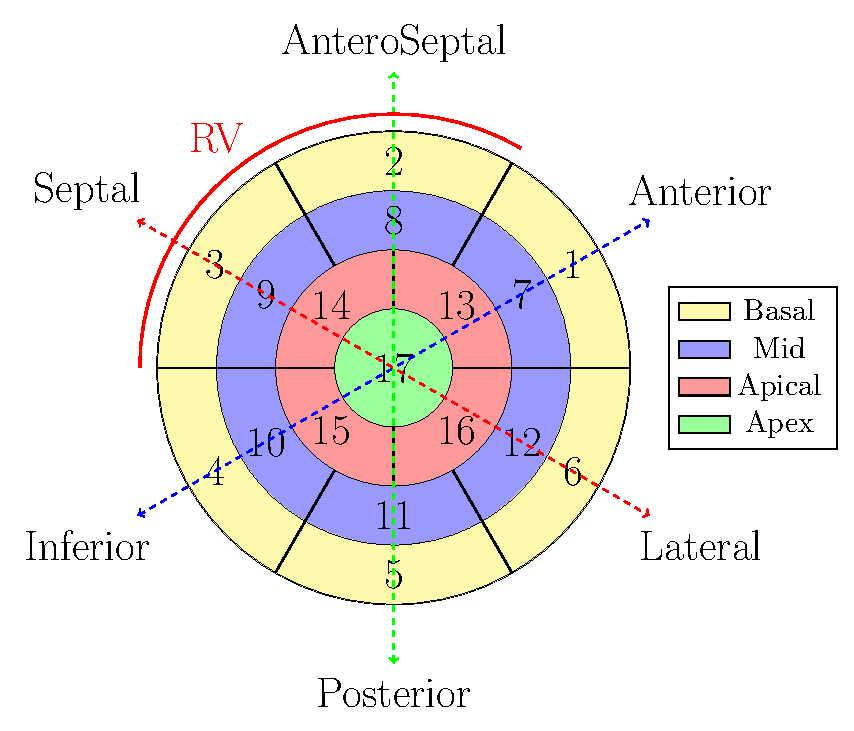
\includegraphics[width=\textwidth]{bullseye}
    \caption{\label{fig:bullseye}}
  \end{subfigure}
\caption{Ventricular geometry generation. Endo and epi-cardial surfaces 
are marked on 3-D ultrasound images. Figure (\ref{fig:ultrasound_image}) shows the endocardial 
marking for a 2-D slice of one such image. Next a computational geometry is generated
from epi and endo-cardial surfaces (\ref{fig:compgeo_mesh}), and rule based
fibers are assigned (\ref{fig:compgeo_fibers}). Finally AHA segments are assigned
to the geometry (\ref{fig:compgeo_regions}), according to the standardized scheme
(\ref{fig:bullseye}).}
\end{figure}

\subsection{Parameter Estimation}
\label{sec:paramest}
Now that we have a mathematical description of cardiac motion, along
with a personalized computational geometry and target data, we next turn to the
problem of personalizing the motion model via the estimation of the
elastic parameters and the fiber contraction. As dyssynchrony is a disease 
which primarily effects the contraction properties of the ventricle,
we focus our efforts on contraction modelling and employ a very simple
personalization of stiffness properties. That is only the parameter $a$
is optimized to fit the ventricular volumes, and the other elastic parameters
are kept fixed at the values ($a_f = 1.685, b = 9.726, b_f = 15.779$),
which were obtained from a bi-axial loading experiment 
[Table 1 row 3 of \cite{Holzapfel2009}].



Fiber contraction varies throughout the cardiac cycle, and so we estimate
the parameter $\gamma$ separately at each time measurements were taken.
Furthermore, as the contraction of the left ventricle may occur dyssynchronously, we
allow for $\gamma$ to vary in space as well as in time.


Muscle shortening is typically present in the ventricles
throughout systole and in early diastole until the muscles fully release
their contraction. During the phase of atrial systole we do not expect
muscle contraction in the ventricle, and so we set $\gamma = 0$ for
this phase. This allows us to estimate elastic properties
independently of contraction during atrial systole, and then estimate
contraction at each point in the rest of the cardiac cycle with the
material parameters fixed. In Figure~\ref{fig:pv_loop_phases} we show
the pressure-volume loop of the patient under consideration, and
highlight the phases where we estimate the contraction and elastic
parameters.

\begin{figure}[htbp]
\centering
    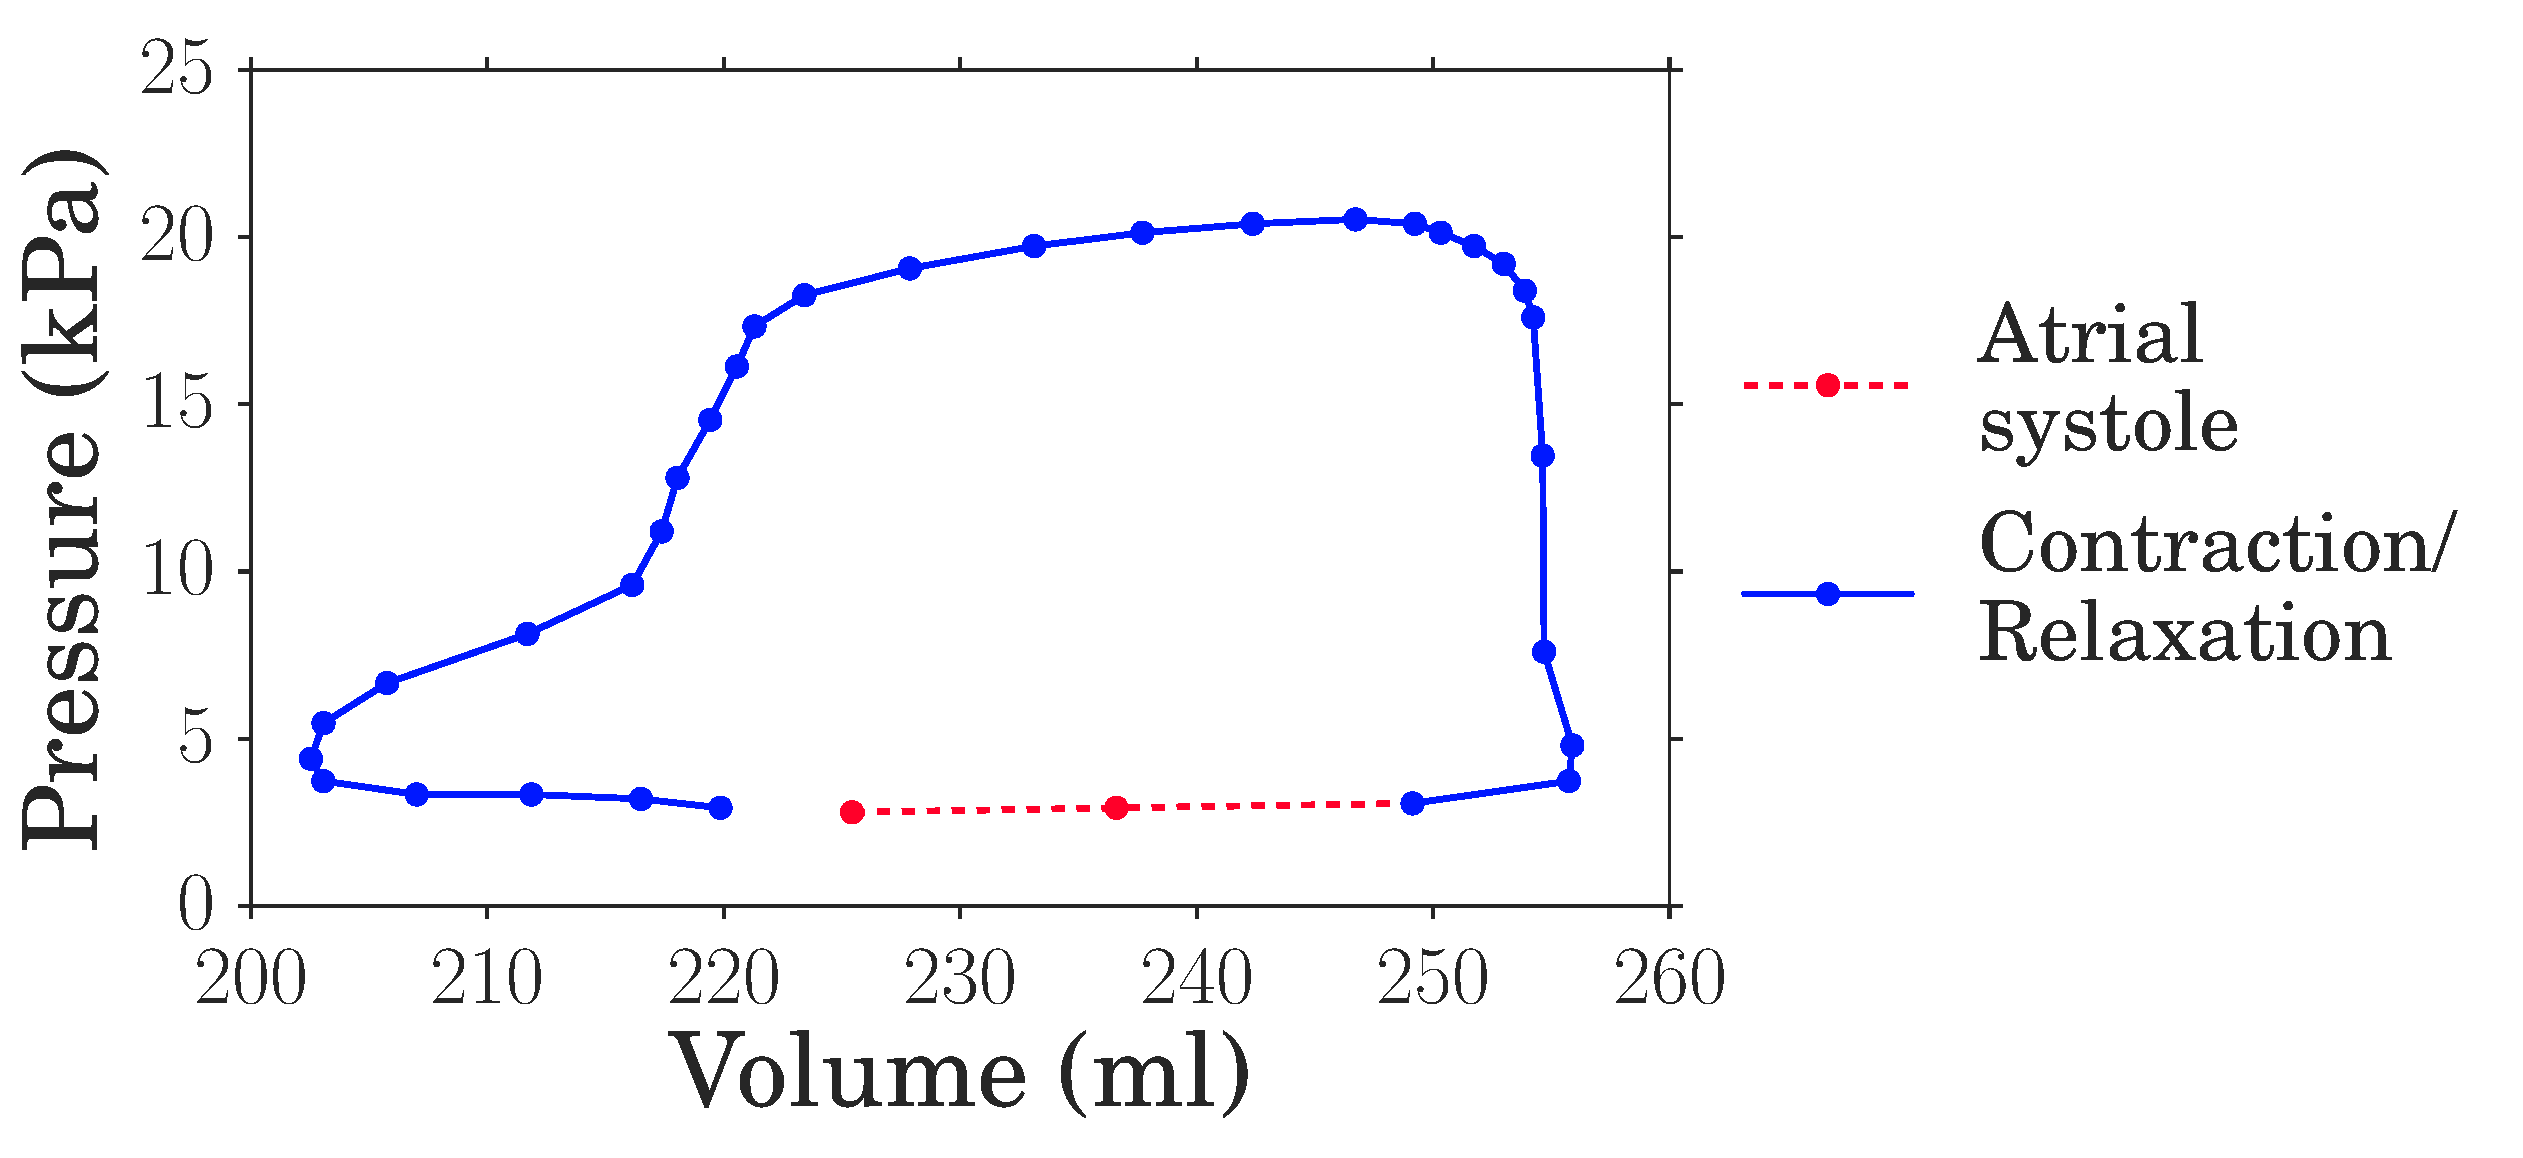
\includegraphics[width=0.8\textwidth]{patient_pv_loop}
\caption{Patient pressure-volume relationship for the left
  ventricle. Measurements in the blue solid line are used to estimate
  contraction, whereas measurements in the red dashed line are used
  to estimate elasticity. }
\label{fig:pv_loop_phases}
\end{figure}


\subsection{Definition of functionals}
\label{sec:data_func}
As described in Section~\ref{sec:clinical_measurements}, the data
available for our personalization of the wall motion model are
pressure, volume and strain measurements throughout the cardiac
cycle. The pressure measurements are included in the model as a boundary condition 
via the virtual work~\eqref{eq:work-balance},
and thus our data assimilation only needs to fit the model to
the volume and strain measurements. This requires that
we define a suitable set of functionals that quantify the
model-strain and model-volume mismatches. The personalization of the wall motion model can
then be achieved by optimizing the contraction and elastic parameters
in order to minimize the total model-data mismatch.

Let $i$ denote the index of an observed cavity volume $V^i$, or strain
$\varepsilon^i$, in the cardiac cycle. Furthermore let $j \in
\{1,..,17\}$ be the index of an AHA segment $\Omega_j$, and $k \in
\{c,r,l\}$ indicate a direction: circumferential, radial or
longitudinal, respectively. Given a measurement point $i$, we define
the model-strain mismatch
\begin{equation}
 \Istrain^i =  \sum_{j= 1}^{17} \sum_{k \in \{c,r,l\}}  \left( \varepsilon_{kj}^i -  \tilde{\varepsilon}_{kj}^i \right)^2,
\label{eq:strain_functional}
 \end{equation}
for model strain $\tilde{\varepsilon}_{kj}^i$ and measured strain
$\varepsilon_{kj}^i$. The speckle tracking software we use provides the measured strain $\varepsilon_{kj}^i$. 
This strain is regionally averaged and of Lagrangian type. In order to mimic this in our model we 
define the model strain as
\begin{equation}
\varepsilon_{kj} =  \frac{1}{|\Omega_j|}\int_{\Omega_j}  \mathbf{e}_k^T \nabla \uvec \, \mathbf{e}_k \ dx,
\label{eq:g_futhese nctional}
\end{equation}
where $\ek$ denotes a unit direction field and
$|\Omega_j|$ the volume of segment $j$.

Furthermore we also define the model-volume mismatch
\begin{equation}
  \Ivol^i  =  \left( \frac{V^i - \tilde{V}^i}{V^i} \right)^2,
\end{equation}
where the model volume is calculated by the formula
\begin{equation}
  \tilde{V}^i = -\frac{1}{3} \int_{\lvendo} (\Xvec + \uvec) \cdotp J \F^{-T} \Nvec  \ dS.
  \label{eq:vol_functional}
 \end{equation}
We note that this method of calculating the model volume depends upon
$(\Xvec + \uvec)\cdotp \Nvec = 0$ at the basal plane. These conditions hold in 
our model as the basal plane is defined with 0 longitudinal coordinate and 
longitudinal displacements are also set to 0 in this plane.

In order to have a single optimization target to describe the fit to data 
we combine the strain \eqref{eq:strain_functional} and volume
\eqref{eq:vol_functional} mismatches into one single functional
\begin{equation}
  \Idata^i(\alpha) = \alpha \Ivol^i + (1 - \alpha) \Istrain^i.
\label{eq:total_functional}
\end{equation}
Here the parameter $\alpha$ controls the relative emphasis of the parameter
estimation on volume or strain matching.

In our study we consider a high dimensional representation of $\gamma$ in order
to more accurately capture the details of a dyssynchronous contraction. However this can easily lead to
an over-parametrized problem in which many parameter combinations produce the same
functional values. In order to further constrain the optimization we introduce
a 1st order Tikohonov regularization functional
\begin{equation}
 \Ismooth^i(\lambda) = \lambda \| \nabla \gamma^i \|^2, 
 \label{eq:I_smooth}
\end{equation}
where $\|\cdotp \|$ represents the standard $L^2$ norm.
This functional discriminates between $\gamma$ parameter sets based on their smoothness.
The parameter $\lambda$ can be adjusted to control the size of the functional and hence
the relative emphasis on smoothing.

\subsection{Parameter estimation as an optimization problem}
\label{sec:param_est}
The elastic parameters of the reduced
Holzapfel-Ogden law \eqref{eq:hoa} represent the passive elastic
properties of the myocardium. We personalize these properties by
adjusting the parameter $a$ to match measured left ventricular volumes.
Mathematically this problem is formulated as
\begin{equation}
\begin{aligned}
\label{eq:opt_matparam}
& \underset{a}{\text{minimize}}
& &  \sum_{i = 1}^{\Nas} \Ivol^i \\
& \text{subject to}
& & \delta W(\plv^i, a) = 0 \quad \forall \,  i \ \in \{1,...N_{AS} \},
\end{aligned}
\end{equation}
where $\delta W$ is given by \eqref{eq:workdef}, and $\Nas =
3$ indicates the total number of measurements available in atrial
systole.

The contraction field that we seek should fit the data as closely as possible while 
also being as smooth as possible. In order to achieve this we minimize both the 
data and smoothness functionals as follows:
\begin{equation}
\begin{aligned}
\label{eq:opt_gamma}
& \underset{\gamma}{\text{minimize}}
& & \Idata^i(\alpha) + \Ismooth^i(\lambda) \\
& \text{subject to}
& &  \delta W(\plv^i, a, \gamma^i) = 0 \quad \\
&&& \gamma^i(\mathbf{X}) \in [0, 1), \ \Xvec \in \Omega.
\end{aligned}
\end{equation}
This problem is solved for every measurement point $i$ not in atrial systole.

The optimization problems \eqref{eq:opt_matparam} and \eqref{eq:opt_gamma} have two
free parameters whose values must be chosen, namely the strain-volume
weighing $\alpha$ and the regularization $\lambda$. The value of $\lambda$ can be expected to influence the trade-off
between the optimized values of the data functional $\Idata^i$ and the regularization functional
$\Ismooth^i$. Similarly $\alpha$ can be expected to influence the trade-off between $\Istrain^i$
and $\Ivol^i$. In our study we choose the values of $\alpha$ and $\lambda$ by examining their effects on the functionals
that they weigh. The choices we made are further described in Section~\ref{sec:a_l_choice}

The spatial resolution of the parameter $\gamma$ affects the amount of detail
that can be captured by the model and simultaneously
the number of variables that need to be optimized. We therefore test 3 different resolutions of $\gamma$.
The lowest resolution, ``scalar'', is simply a single global value.  The next resolution
is ``regional'', and consists of a separate value for each of the 17 AHA zones. Finally, the highest resolution
we consider is ``P1'' and consists of a separate value at each of the vertices of the mesh,
with a linear interpolation between vertices. Using our ventricular mesh, a P1 resolution of $\gamma$ has 1262 separate variables.


\subsection{Implementation of mechanics and optimization solvers}
For the numerical solution of the work balance equation~\eqref{eq:work-balance} we employ a
Galerkin finite element method with Taylor-Hood tetrahedral
elements~\cite{hood1974navier}; that is, a continuous piecewise
quadratic representation of the displacement field and a continuous
piecewise linear representation of the pressure field.  

The software implementation of our finite element method is based on
the package FEniCS~\cite{LoggMardalEtAl2011a}, which automatically
generates matrix and vector assembly code from a symbolic
representation of the work balance equation~\eqref{eq:work-balance}.
The resulting nonlinear systems were solved using the PETSc
implementation of a Newton trust region algorithm~\cite{PETScPackage},
while the inner linear solves were handled by a distributed memory
parallel LU solver~\cite{lidemmel03}.

To solve the optimization problems \eqref{eq:opt_matparam} and
\eqref{eq:opt_gamma}, we apply a sequential quadratic programming
algorithm (SQP)~\cite{kraft1988software}. This algorithm requires the
derivatives of the function to be optimized, which in our case are the
gradients of the mismatch functionals in
problems~\eqref{eq:opt_matparam} and \eqref{eq:opt_gamma} with respect
to $a$ and $\gamma$ respectively. These gradients are
automatically computed by solving a machine derived adjoint equation via the
software framework dolfin-adjoint~\cite{farrell2013automated}.

In addition to gradients, the SQP algorithm requires evaluations of
the mismatch functionals for given values of the control variables,
which again relies on the solution of the work balance
equation~\eqref{eq:work-balance}. In the case of
problem~\eqref{eq:opt_gamma}, the control variable is $\gamma$, which
has a large influence on the solution of \eqref{eq:work-balance}.
Numerical solution of \eqref{eq:work-balance} by Newton's method
depends upon having a good initial guess, which in our case are the
values of the mechanical state variables, $\uvec, p$, resulting from
the previous solve of \eqref{eq:work-balance}. If the value of
$\gamma$ differs too greatly from one solve to the next the Newton
algorithm might fail due to the root of the system being too far away
from the initial guess. To avoid this problem we make use of a
homotopy procedure that moves from one value of $\gamma$ to the next
in small increments, and solves \eqref{eq:work-balance} each time the
value of $\gamma$ is changed.  This procedure is presented as
Algorithm~\ref{alg:homotopy-newton} and is similar to the one found
in~\cite{pezzuto2014orthotropic}. 

All algorithms, solvers and relevant data are
publicly available online \cite{OurPackage}.

\begin{algorithm}
\caption{Max Increment Homotopy Newton Solver}
\label{alg:homotopy-newton}
  \begin{algorithmic}
   \State \emph{Initial Variables}
   \State $\begin{array}{ll}
    \quad \uvec_{prev} & \quad \quad \quad  \mbox{Previous displacement field} \\
    \quad p_{prev} & \quad \quad \quad  \mbox{Previous tissue hydrostatic pressure field} \\
    \quad \gamma_{next} & \quad \quad \quad  \mbox{Desired tissue contraction field} \\
    \quad \delta \gamma_{max} & \quad \quad \quad  \mbox{Maximum change in a component per Newton solve}
   \end{array}$

   \\
   \State \emph{Set}
   \State \quad $\gamma_0 = \gamma_{prev}$
   \State \quad $\uvec_0 = \uvec_{prev}$
   \State \quad  $p_0 = p_{prev}$
   \State \quad  $M = \left \lceil \frac{\|\gamma_{next} - \gamma_{prev}\|_{\infty}}{\delta \gamma_{max}} \right \rceil$
   \State \quad $\delta \gamma = \frac{1}{M}(\gamma_{next} - \gamma_{prev})$
   \\
   \State \emph{Use Newton's method $M$ times with fixed increment $\delta \gamma$}
   \For{$i \in \{1...M\}$}
      \State $\gamma_i = \gamma_{i -1} + \delta \gamma$
      \State Initialize Newton solver with $\uvec_{i -1}, p_{i -1}$
      \State Solve $\delta W(\uvec_i, p_i, \gamma_i) = 0$ for $\uvec_i, p_i$
   \EndFor
   \State Output $\uvec_i, p_i$
  \end{algorithmic}
\end{algorithm}

\subsection{Error Estimation}

The optimization functionals introduced in Section~\ref{sec:data_func} are defined 
separately for each measurement
point. For the purposes of evaluating goodness of fit over the entire cardiac cycle
we consider metrics that are averaged over measurement points. Furthermore we 
relate errors to the sizes of the data 
for ease of interpretation. In the case of the model-volume error we introduce the volume metric
\begin{equation}
\overline{I}_{\text{vol}} = \frac{ \| V^i - \tilde{V}^i \|_{\ell^1}}{ \| V^i \|_{\ell^1}}
\label{eq:average_volume}
 \end{equation}
where the $\ell^1$ norm is taken with respect to the measurement point index $i$.
Furthermore we consider two average strain metrics
\begin{align}
\Istrainavg &= \frac{1}{51} \sum_{j= 1}^{17} \sum_{k \in \{c,r,l\}}
\frac{\| \varepsilon^i_{k,j} -  
\tilde{\varepsilon}^i_{k,j} \|_{\ell^1} }{ \| \varepsilon^i_{k,j} \|_{\ell^1}}, \\
\Istrainrelmax &=  \frac{1}{51} \sum_{k \in \{c,r,l\}}
 \frac{\sum_{j= 1}^{17} \| \varepsilon^i_{k,j} 
 -  \tilde{\varepsilon}^i_{k,j} \|_{\ell^1}}{ \max_j \| \varepsilon^i_{k,j} \|_{\ell^1}}.
\label{eq:average_strain}
\end{align}
Here $N$ specifies the number of measurement points used in the
optimization, and the factor $51$ is $17 \times 3$,
the number of AHA segments times the number of strain measurements per segment. 
The first metric considers relative differences between norms, whereas the second relates 
errors norms to the maximum
strain norm over all segments. This second metric emphasizes larger features in 
the strain curves more heavily, and deemphasizes
small scale features such as noise.

Similarly to the average data errors introduced above we also introduce a smoothness 
metric that is averaged across measurement points
\begin{equation}
\overline{I}_{\text{smooth}} = \frac{1}{N}\sum_{i = 1}^N \Ismooth^i, \\
\end{equation}
and a combined data metric based on the strain and volume metrics
\begin{equation}
  \Idataavg = \Ivolavg + \Istrainavg.
\label{eq:total_functional}
\end{equation}

Finally we also define an error metric for a synthetic
data test of the contraction optimization \eqref{eq:opt_gamma}. In this
test a contraction field $\gamma_{\text{ground}}$ is chosen and 
synthetic data is generated from the 
mechanics model. This data is then used to calculate a
reproduction of the contraction $\gamma_{\text{repr}}$. 
In order to compare the ground truth and reproduced contraction 
fields we employ a relative $L^2$ norm
\begin{equation}
  \| \epsilon_{\gamma} \|_{\text{avg}} = \frac{1}{N} \sum_{i = 1}^{N}  \frac{\| \gamma_{\text{repr}}^{i} -
  \gamma_{\text{ground}}^{i} \|_{L^2}}{ \| \gamma_{\text{ground}}^{i} \|_{L^2}}.
\label{eq:error_gamma}
\end{equation}

\section{Numerical Experiments}
\label{sec:num_results}
In this section we present the results of our numerical experiments.
We first estimate the parameter $a$ using volume measurements in atrial systole.
We then test the estimation of contraction $\gamma$ using synthetic data generated
by the wall motion model. This gives an idea of how well the algorithm
can perform under idealized circumstances.  Next, we
carry out the contraction estimation using the clinical strain and volume data.
Finally, we consider lower resolution representations of $\gamma$, and compare 
the resolutions based on computational expense and data matching capability.

In all of the experiments below, optimizations were terminated if the
difference between the value of the mismatch in the current and
previous iteration was less than $10^{-9}$ for the passive material
parameter optimization and $10^{-6}$ for the contraction
parameter optimization or if the
SQP algorithm was not able to further reduce the mismatch value.
In the active parameter optimization the SQP
algorithm was initialized with the value of $\gamma$ from the previous
measurement point in the cardiac cycle. 

In order to obtain convergence of Newton's method for the solution of
the virtual work equation~\eqref{eq:work-balance}, we set $\delta
\gamma_{max} = 0.02$ in the homotopy Newton solver
(Algorithm~\ref{alg:homotopy-newton}), and 
limit $\gamma$ to the interval $[0, 0.9]$. In the cases that Newton's
method did not converge, $\delta \gamma_{max}$ was halved until convergence was obtained. 

Strains were calculated with respect to the measurement point defined
as start of atrial systole, as the reference geometry taken from the
image corresponding to this point was assumed to be stress and strain
free. Similarly, pressures for the clinical data were adjusted
downward by the pressure measured at the start of atrial systole, 2.8
kPa, so that the adjusted start of atrial systole pressure was 0, and
therefore compatible with the stress free assumption.

The value of the basal spring-constant was set to $k = 1.0$ kPa. This allowed for some
motion in the basal plane,
and was shown in a sensitivity analysis (see Appendix~\ref{sec:k_sense})
to give optimal $\gamma$ values
whose spatial average is close to that obtained with a completely fixed boundary.

\subsection{Estimation of elastic parameter $a$}
\label{sec:elasticparam}
An estimate of the parameter $a$ was obtained by minimizing the mismatch between
model derived and clinically measured volumes in atrial systole,
as described in \eqref{eq:opt_matparam}. The optimal $a$ value obtained was $0.435$, 
with goodness of fit $\overline{I}_{\text{vol}} = 0.0035$.
The same optimal $a$ value was obtained from 8 randomly chosen starting points
between 0 and 45.


\subsection{Synthetic dataset creation}

\label{sec:data_synthetic}
In order to evaluate the performance of our contraction estimation
method \eqref{eq:opt_gamma} under idealized conditions we  
have performed synthetic data tests. The data for these tests was
constructed by solving the virtual work 
equation~\eqref{eq:work-balance} for a given set of elastic parameters
 $(a, a_f, b, b_f)$, contraction $\gamma$, and cavity pressures.
The $a$ parameter was set to $0.435$, as obtained previously by
fitting the model to the patient atrial systolic volume data. The
other three elastic parameters were fixed to the values mentioned in Section~\ref{sec:paramest}.
The contraction $\gamma$ was chosen to be a wave 
with Gaussian shape and P1 resolution traveling along the longitudinal axis.

Eight points of measurement were used in the synthetic tests. This was
fewer than the number of in-vivo  
measurement points, which allowed for faster computations. The
pressure values that were chosen  
for the synthetic measurement points
can be seen in Figure~\ref{fig:synthetic_gammafields}. These pressures start at 0, 
increase to the maximum atrial systole pressure 
that was measured in-vivo and then decrease linearly back to 0. 


For the synthetic strain data we considered three different cases. The
first case consisted of the displacement  
gradient tensor defined over the entire ventricular geometry. Next we
considered regionally averaged values of the 
diagonal components of the displacement gradient. The regional averaging mimics the
strain curves generated by the speckle tracking software.  
Finally we consider 30 noisy realizations of the regional strain
curves. The noise that was added to these curves was estimated 
from the drift values of the in-vivo strain and is described in
Appendix~\ref{sec:strain_noise_est}.


\subsection{Choice of functional weights $\alpha$ and $\lambda$}
\label{sec:a_l_choice}
The optimization functional weights $\alpha$ and $\lambda$ were chosen based on
trial optimizations using the synthetic and in-vivo datasets. The strains in the synthetic
data were regionally averaged and noisy.
In these trials we first set $\lambda = 0$ and tested $\alpha$ values
ranging from 0 to 1.0 in increments of 0.1, in addition to the values
0.95, 0.99, 0.999, and 0.9999.
For each level of $\alpha$ we recorded the values of the
fit metrics, $\Ivolavg$ 
and $\Istrainavg$, and plotted them against each
other (Figure~\ref{fig:lcurves}). Based on the plot 
we chose $\alpha = 0.95$ as this value gave a good balance between
volume and strain matching.  
With the value of $\alpha$ fixed to $0.95$ we tested $\lambda$
from $10^{-6}$ to $100.0$ in increasing powers of 10.
The effect of the choice of $\lambda$ on the smoothness and data functionals
is shown in Figure~\ref{fig:lcurves}. Based on this plot we selected points
that gave near optimal fit values with a high level of smoothness. 
These points were $\lambda = 1.0$ for the synthetic case
and $\lambda = 0.01$ for the patient case.



\subsection{Contraction estimation with synthetic data}
\label{sec:results_synthetic}
Using the synthetic datasets described in Section \ref{sec:data_synthetic} as a target we 
calculated optimized contraction fields. All elastic parameters 
were kept fixed throughout the optimization so that the test was restricted to
the contraction field.
We quantified the error in the reproduction of $\gamma$ using P1
resolution for the three cases of strain. Errors in the relative norm, $\| \epsilon_{\gamma} \|_{\text{avg}}$,
were 0.033 for the full displacement gradient tensor and 0.227 for the 
regionally averaged diagonal of the displacement gradient without noise. The average error
for the 30 noisy regionally averaged cases was 0.224 with a standard deviation of 0.009.
We note that the reproduction error was lowest for the full clean strains, 
and an order of magnitude higher
for the regional clean and regional noisy strains. We also note that the 
reproduction error using regional clean strains was very
close to the average reproduction error from the 30 regional noisy strains.
The maximum error for all three cases of strain occured in the apex, 
and was 0.06, 0.0701, 0.0724 for the full, regional clean and regional noisy cases
respectively.



For the case of the full clean strains we have plotted the 
reconstructed contraction field alongside the ground truth in
Figure~\ref{fig:synthetic_gammafields}. 
We note that the ground truth and reproduction appear very similar. In
order to visualize the effect of the  
noise in strain on the optimized contraction field we
plotted the mean and standard deviation of the 30 synthetic strain curves,
and mean and standard deviation of the average of the contraction field 
resulting from the 30 strain curves. Both of these plots are
restricted to the anterior basal segment and are shown in Figure
\ref{fig:noisy_strain_curve}. We note that the effect of the noise on
the average contraction field is minimal.


\begin{figure}[htbp]
\centering
\begin{subfigure}[t]{0.49\textwidth}
  \caption*{\Large{Synthetic}}
     \includegraphics[width=0.845\textwidth]{{l_curve_fixed_lambda_0.0_synth_w_noise}.eps}
\end{subfigure}
\begin{subfigure}[t]{0.49\textwidth}
  \caption*{\Large{Patient}}
  \includegraphics[width=\textwidth]{{l_curve_fixed_lambda_0.0_patient}.eps}
\end{subfigure}
\begin{subfigure}[t]{0.49\textwidth}
     \includegraphics[width=0.845\textwidth]{{l_curve_fixed_alpha_0.95_synth_w_noise}.eps}
\end{subfigure}
\begin{subfigure}[t]{0.49\textwidth}
  \includegraphics[width=\textwidth]{{l_curve_fixed_alpha_0.95_patient}.eps}
\end{subfigure}
\caption{Trade-off curves for various $\alpha$ and $\lambda$ values
  used in model personalization with synthetic strain data and in-vivo patient data.
  The synthetic strains are noisy and regionally averaged. The contraction parameter is represented 
  at P1 resolution.
  Top:
  optimal strain mismatch \eqref{eq:average_strain} versus average volume mismatch \eqref{eq:average_volume} 
  for a range of $\alpha$ values and $\lambda = 0.0$.  Bottom: Total data mismatch
  versus contraction gradient size for a range of $\lambda$ values
  and $\alpha = 0.95$.}
\label{fig:lcurves}
\end{figure}
% 
\begin{figure}[htbp]
  \begin{subfigure}[t]{0.5\textwidth}
    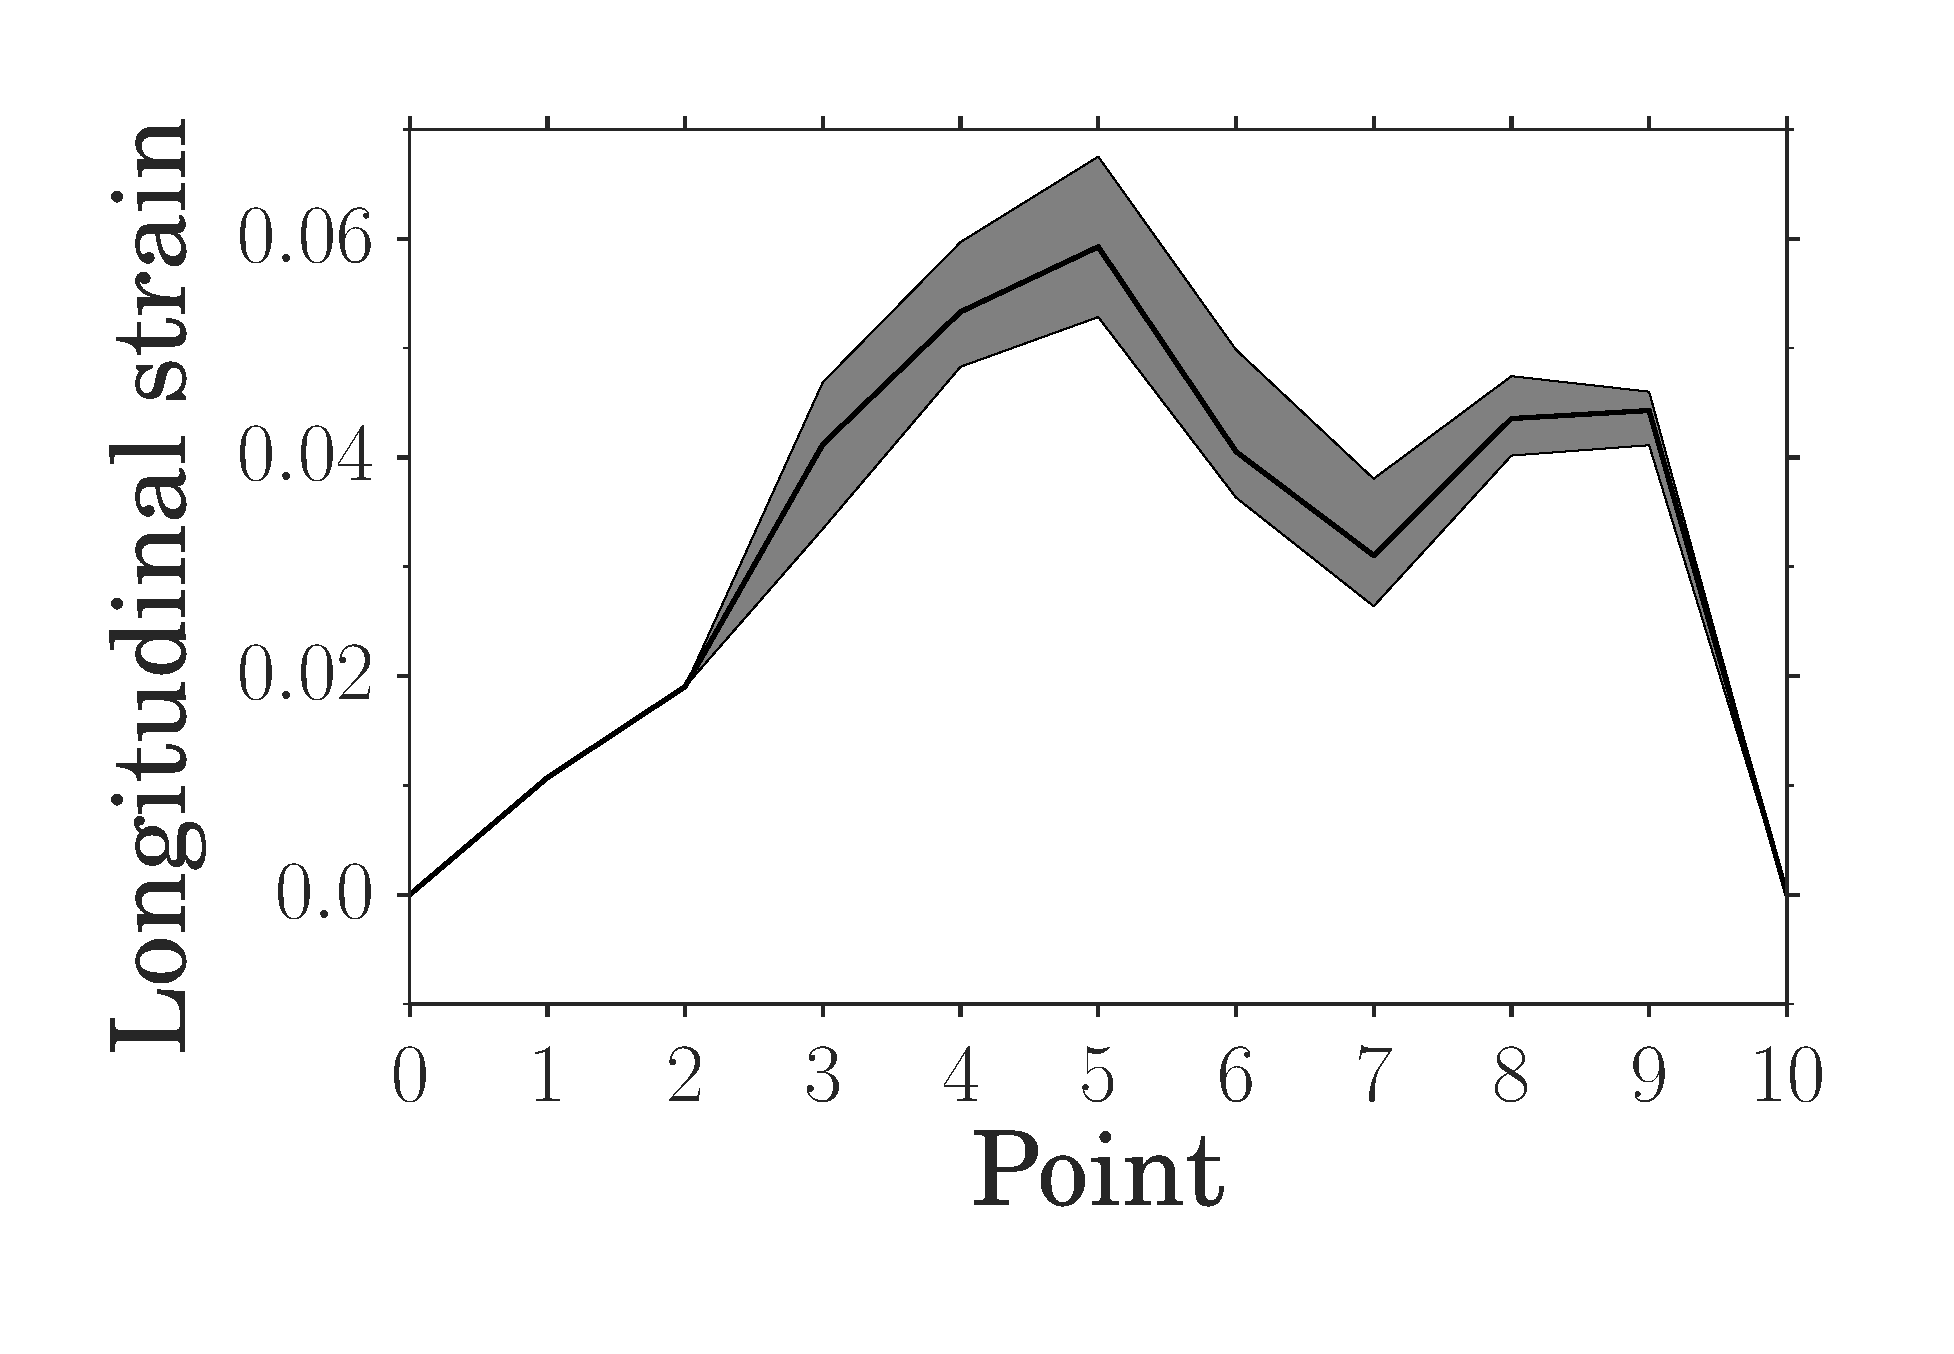
\includegraphics[width=\textwidth]{noisy_strain_region_1_ground.eps}
  \end{subfigure}
  \begin{subfigure}[t]{0.41\textwidth}
    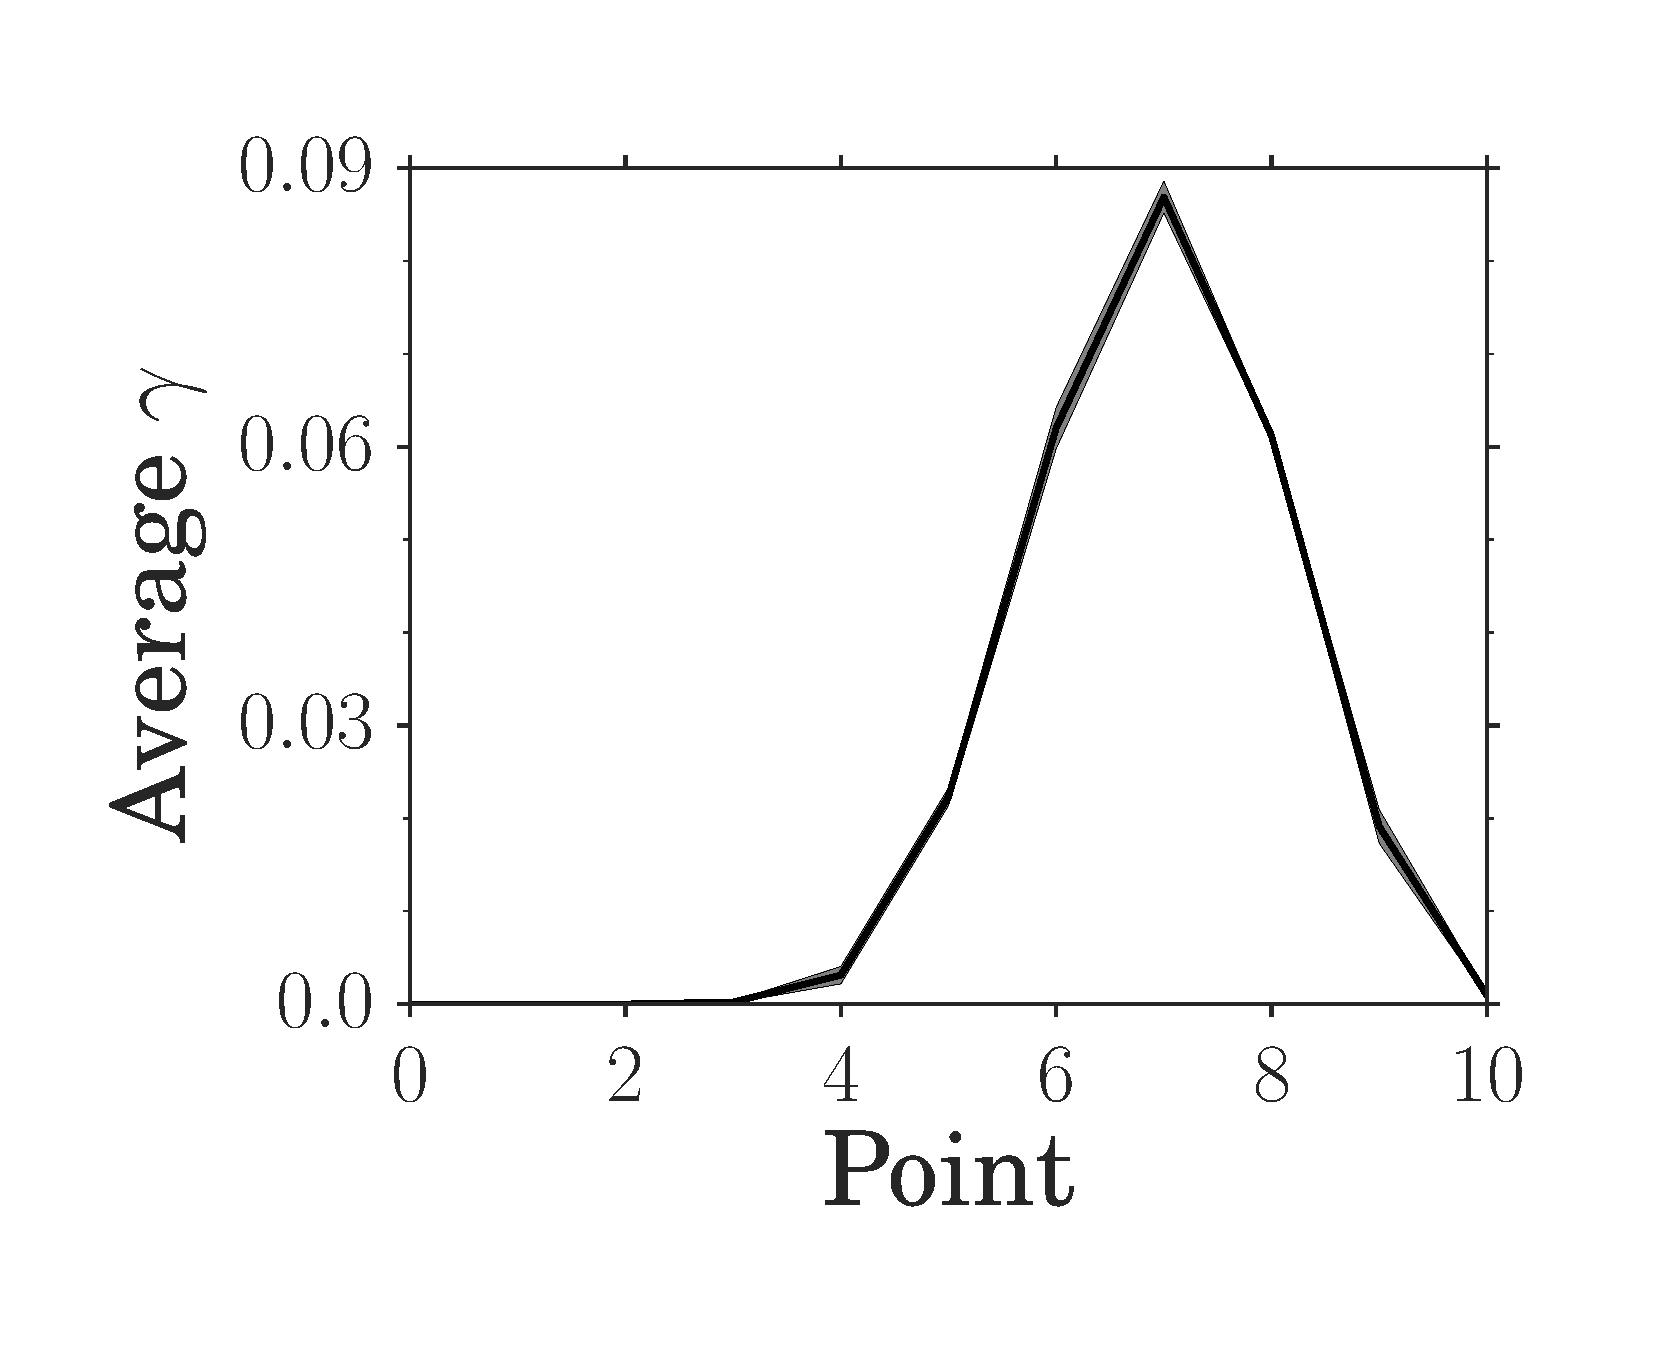
\includegraphics[width=\textwidth]{mean_gamma_region_1_synth_w_noise.eps}
  \end{subfigure}
\caption{
On the left are the mean (solid line) and standard deviation (highlighted area) of 30
synthetic longitudinal strain curves in the anterior basal segment corrupted by Gaussian noise.
On the right are the mean and standard deviations of
$\gamma$ averaged over the same segment.}
\label{fig:noisy_strain_curve}
\end{figure}


\begin{figure}[htbp]
 \includegraphics[width=1.0\textwidth]{synthetic_gamma_snapshots.eps}
 \caption{Lateral view of the ground truth and reconstructed contraction fields at 7 measurement points during
  the synthetic data test. The target for the optimization is the full strain field with no noise.
 At each pressure the reconstruction is displayed on the left and the ground truth on the right.}
\label{fig:synthetic_gammafields}
 \end{figure}

\subsection{Contraction estimation with in-vivo data}
\label{sec:results_clinical}

Using the in-vivo data described in
Section~\ref{sec:clinical_measurements} as a target, we calculated optimized contraction 
fields at P1 resolution. These contraction fields are shown in
Figure~\ref{fig:snap_shots}. We note that the value of the contraction varies significantly in space and time.
A comparison of the estimated to the measured PV loop is shown in Figure~\ref{fig:pv_match}. Optimized
and measured strains are compared in Figure~\ref{fig:strain_match}.

\begin{figure}[htbp]
\centering
  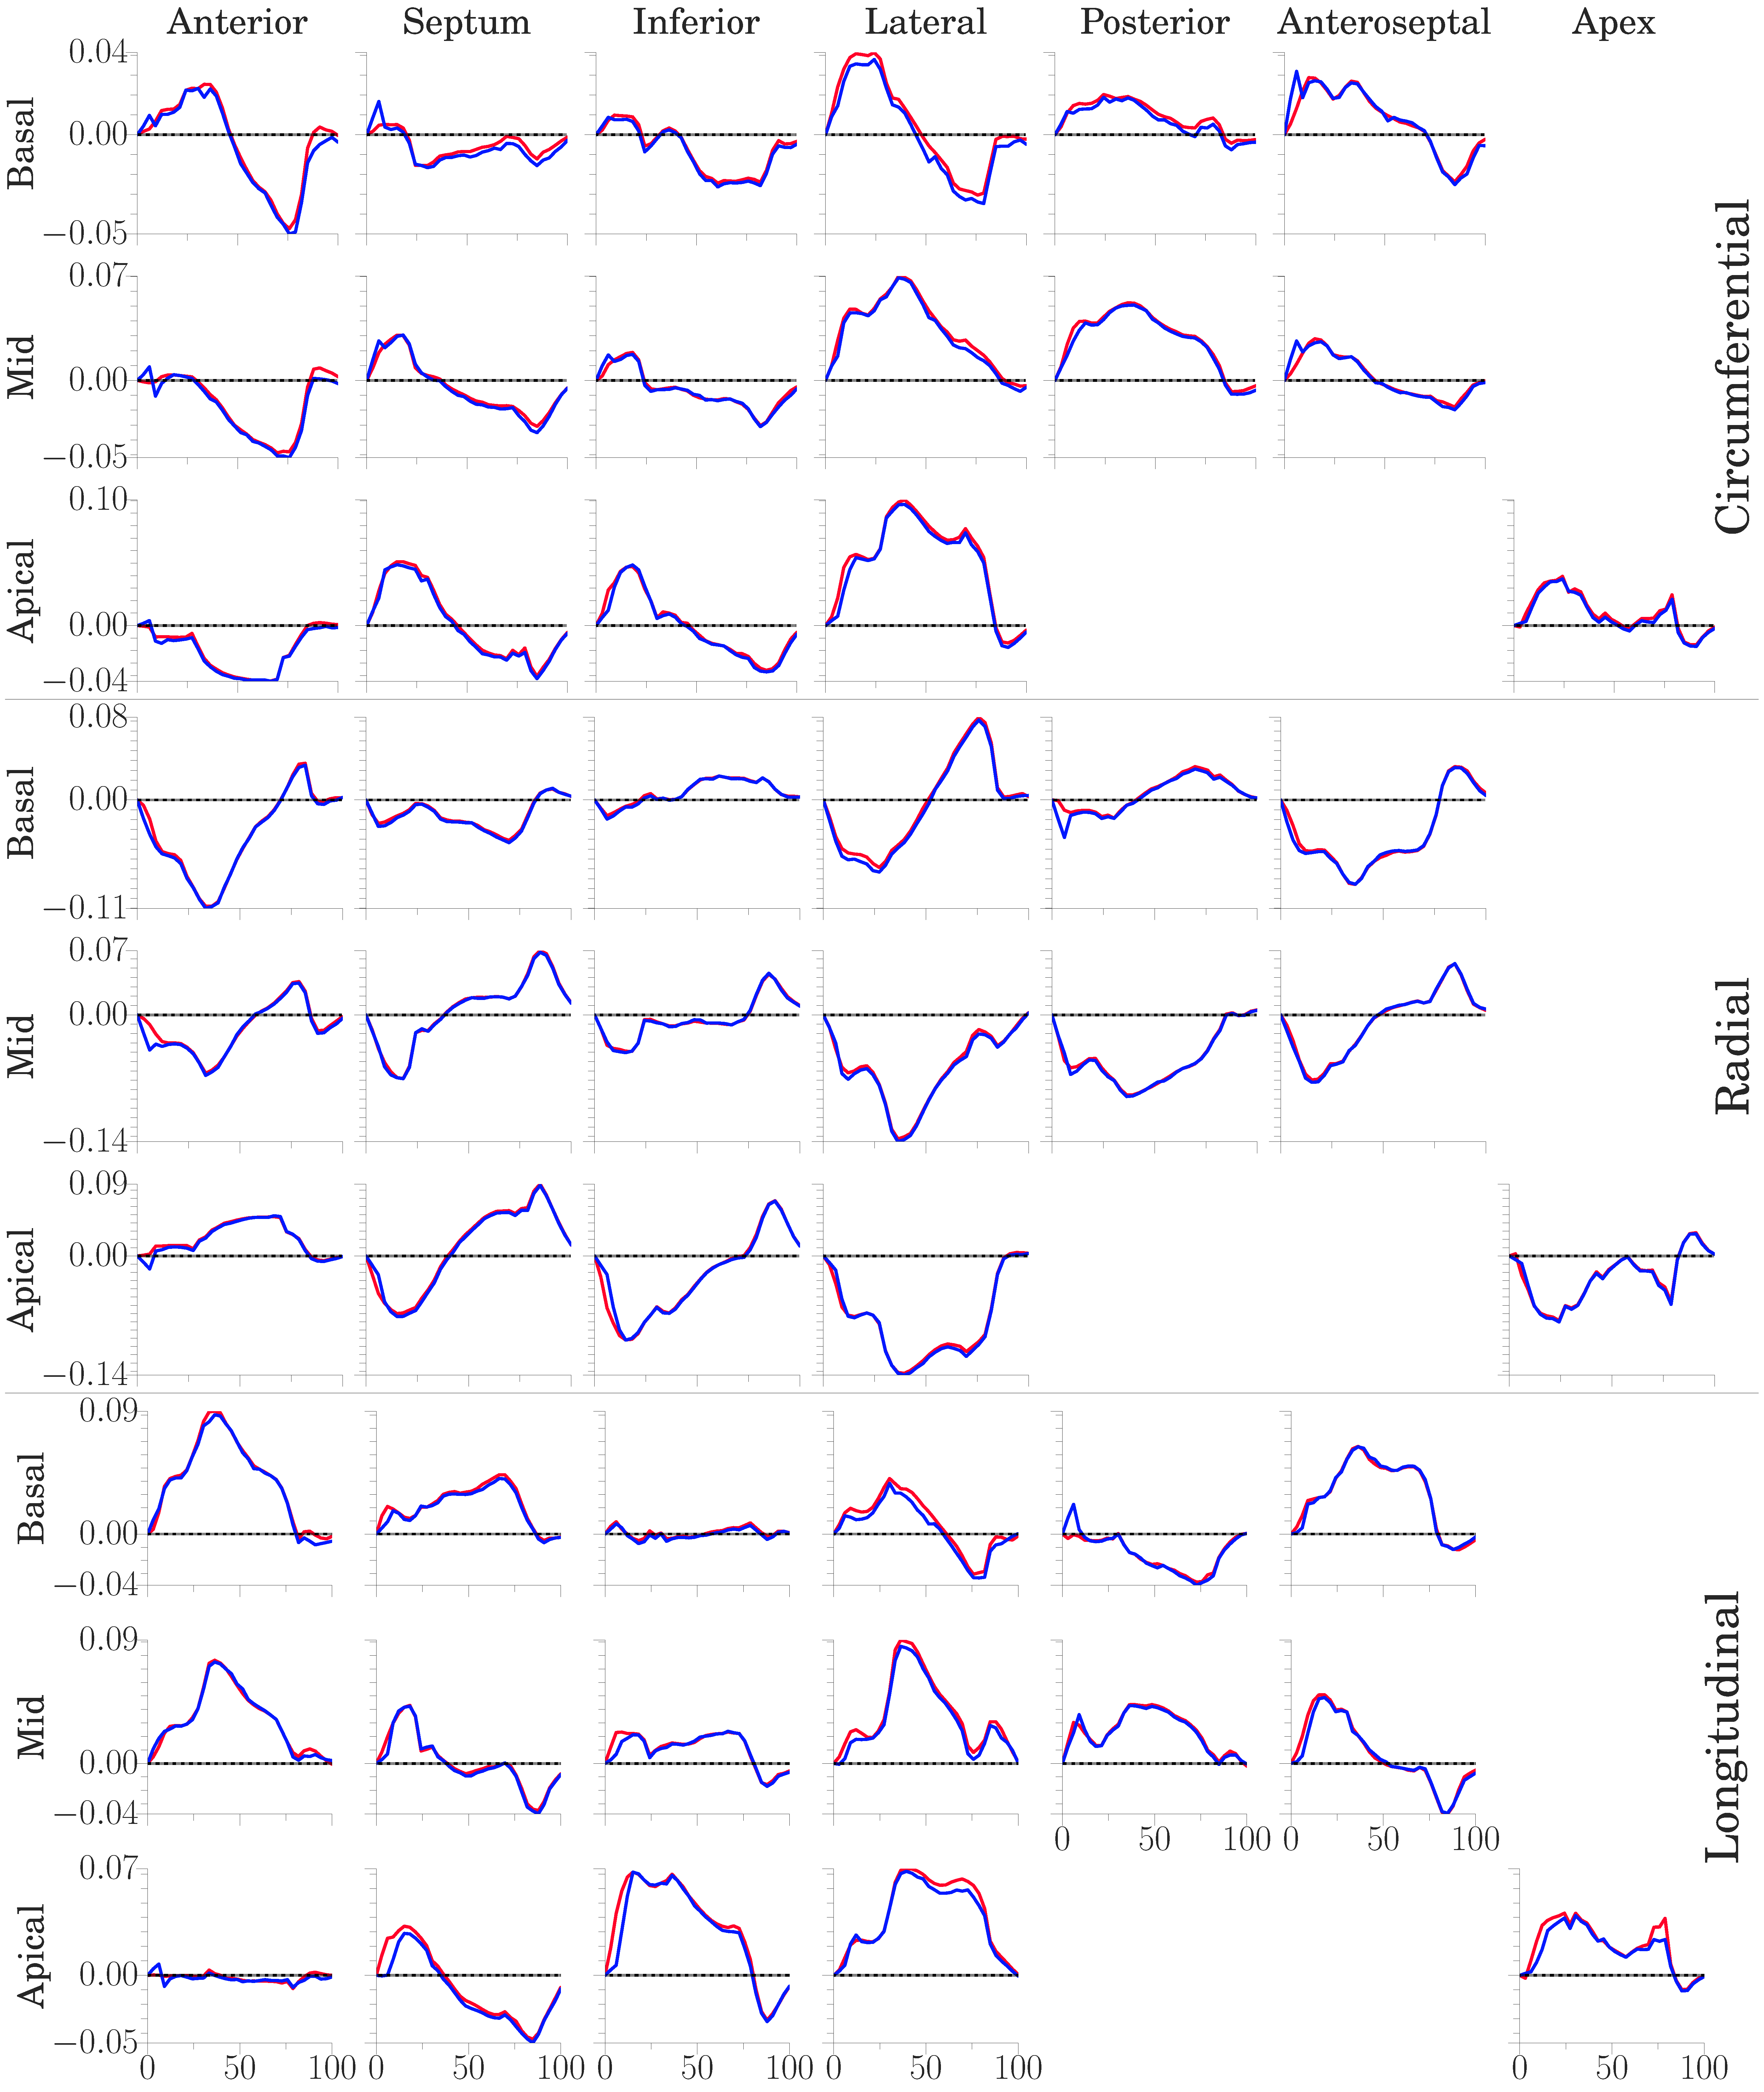
\includegraphics[width=\textwidth]{simulated_strains}
\caption{Comparison of regional strain curves starting in end diastole. In red: optimized wall
  motion model data. In blue: clinical data from speckle tracking
  echocardiography. In each plot the $y$-axis represents strain while
  the $x$-axis shows the progression in time of the cardiac cycle as a
  percentage.}
  \label{fig:strain_match}
\end{figure}

\begin{figure}[htbp]
\centering
    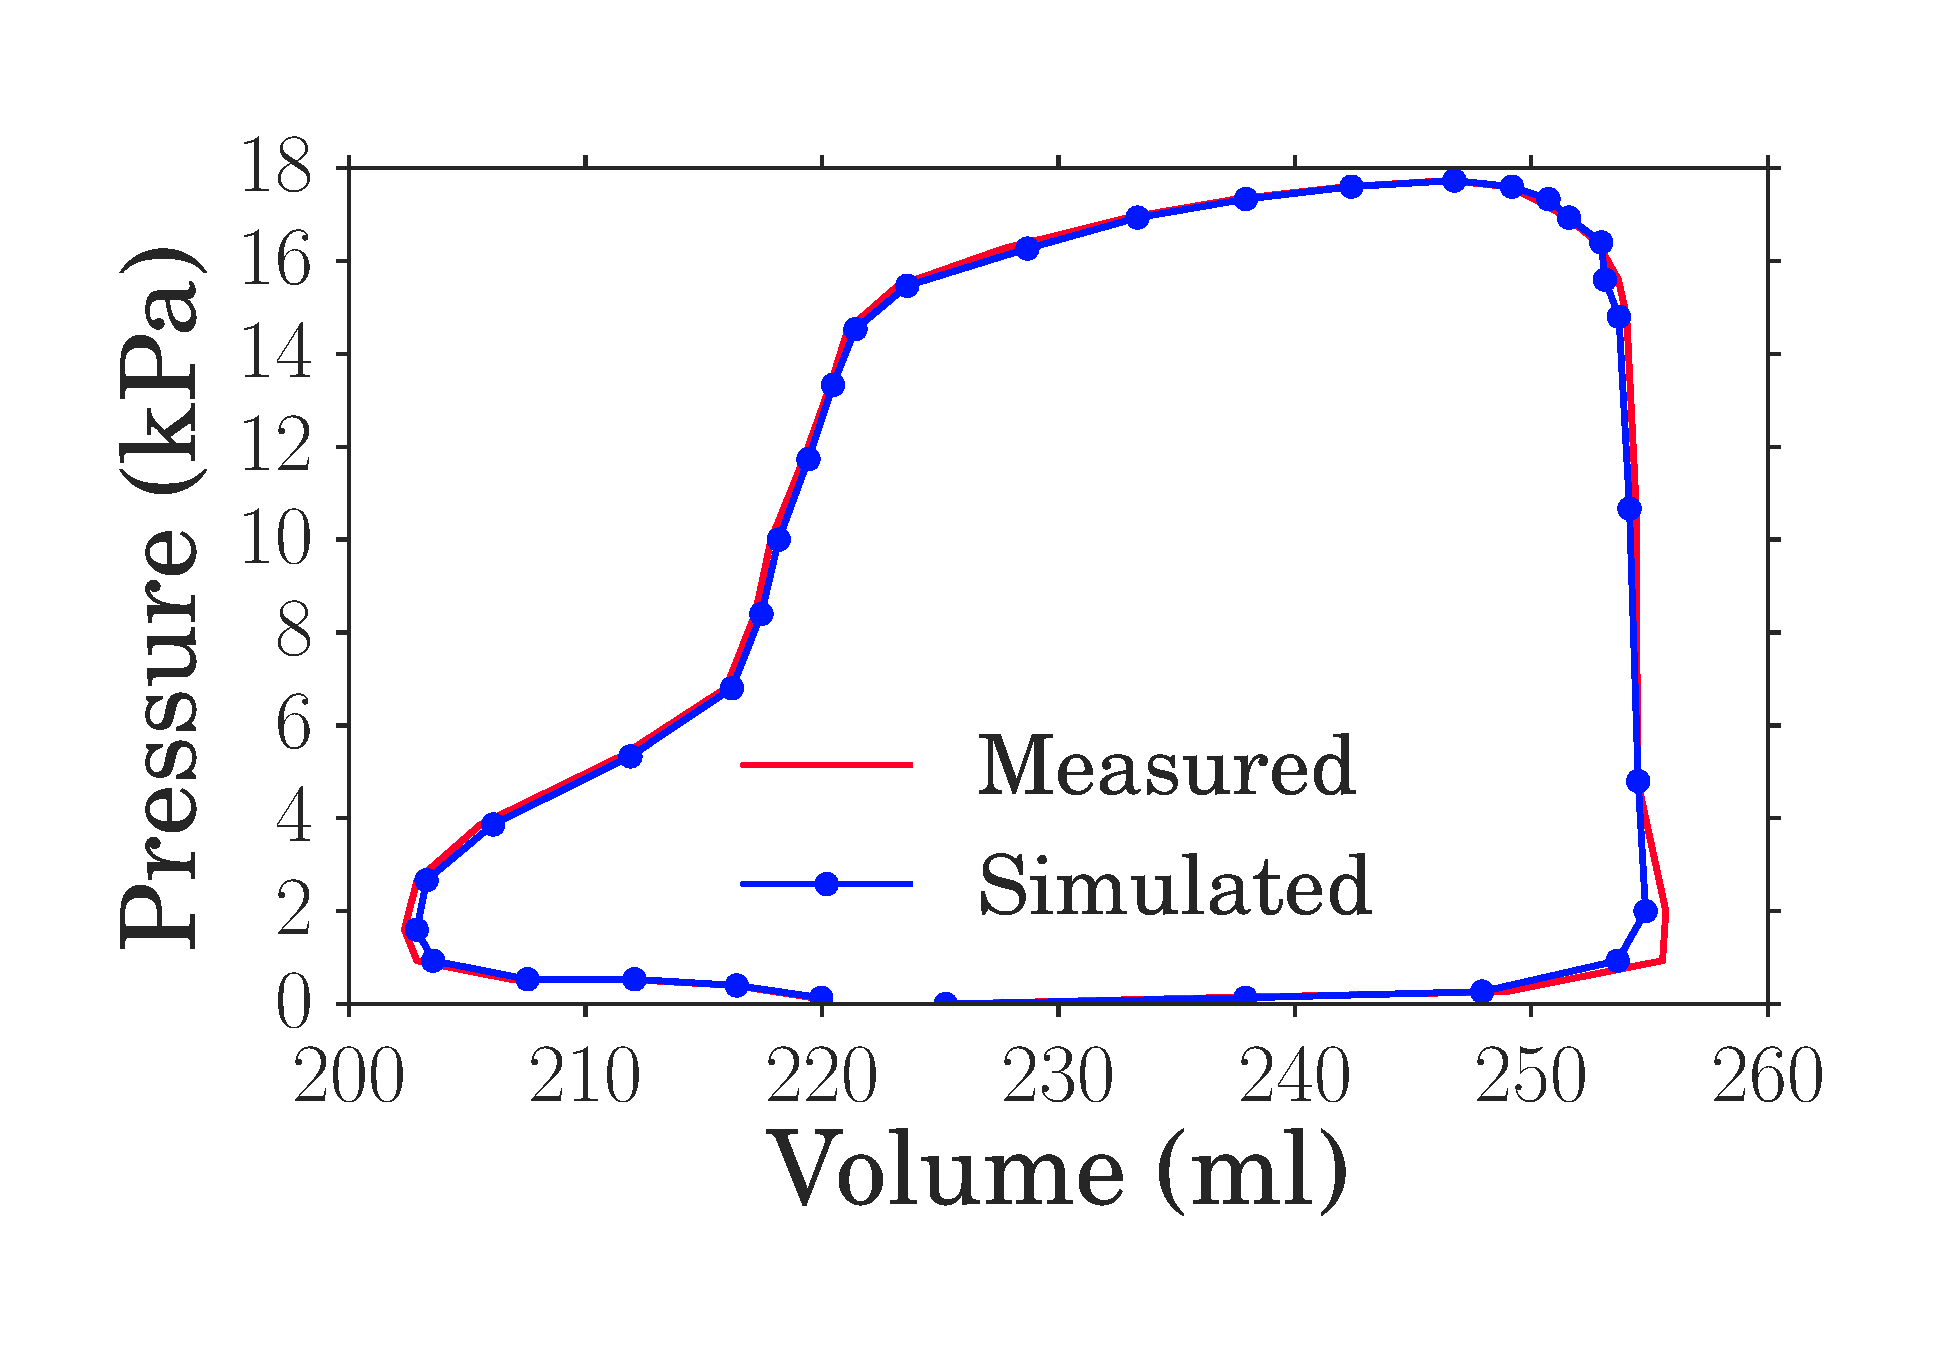
\includegraphics[width=0.7\textwidth]{simulated_pv_loop}
\caption{Clinically measured (red) versus optimized wall motion model
  (blue) left ventricular cavity volumes.}
\label{fig:pv_match}
\end{figure}

\begin{figure}[htbp]
\centering
    \includegraphics[width=\textwidth]{patient_gamma_snapshots}
\caption{Posterior view of the contraction field $\gamma$ optimized to in-vivo data 
at P1 resolution. A snapshot is shown for every third in-vivo measurement point.}
\label{fig:snap_shots}
\end{figure}


\subsection{Effect of contraction parameter resolution}
In order to quantify the effects of the resolution of the contraction field $\gamma$
we have repeated the contraction estimation from in-vivo data using regional and scalar resolutions.
The fit values obtained for these resolutions are compared to the fit value of the P1 resolution in Table~\ref{tab:gamma_space_opt_misfit}.
The results show that the P1 resolution of $\gamma$ gives an order of magnitude better strain and volume
matches than the scalar and regional resolutions, and that $\Istrainrelmax$
is about an order of magnitude lower than $\overline{I}_{\mathrm{strain}}$ in all three cases.

The computational cost of the data assimilation using the three resolutions of $\gamma$ is compared in 
Table~\ref{tab:patient_opt_details}. We note that the number of forward and adjoint solves 
increases with the resolution and that the average runtime of an adjoint solve in the scalar and P1 resolutions
are almost the same.

\begin{table}
  \centering
\caption{Performance of the contraction optimization with the clinical data for different
resolutions of contraction parameter $\gamma$.
The second and third column display the average number of forward and adjoint solves required to
optimize $\gamma$ at a single measurement point. The fourth column shows the total run time over all measurement points and
the final column the average run time of an adjoint solve. }
\begin{tabular}{lrrrr}
\hline
 resolution of $\gamma$ & forward solves &    adjoint solves &   total run time (s)  & adjoint evaluation \\
                       &  average        & average           &                       & average run time (s) \\
\hline
 scalar                &                   4.6  &                   2.8 &    280   & 7.4 \\ %(0.082) 
 regional              &                   12   &                   6.5 &    210   & 19.3 \\ %(0.062)
 P1                    &                   46   &                   46  &    1100  & 7.9 \\ %(0.11)
\hline
\end{tabular}
\label{tab:patient_opt_details}
\end{table}



\begin{table}
\caption{Relative misfit for different representation of $\gamma$}
\begin{tabular}{lrrr}
\hline
 resolution of $\gamma$ &   $\Ivolavg$ &   $\Istrainavg$  &    $\Istrainrelmax$ \\
\hline
 scalar           &                          0.044  &                                              1.5  &                                             0.27  \\
 regional         &                          0.024  &                                              1.1  &                                             0.16  \\
 P1               &                          0.0037 &                                              0.17 &                                             0.029 \\
\hline
\end{tabular}
\label{tab:gamma_space_opt_misfit}
\end{table}



\section{Discussion}
\label{sec:discussion}
In our study we have created a personalized model of whole cycle ventricular mechanics
based on strain, volume and pressure measurements of a dyssynchronous left ventricle. 
The contraction parameter in our study was resolved at a high P1 level of resolution.
Previous studies \cite{wong2015velocity, chabiniok2012estimation} have considered
contraction parameters that were resolved up to the regional level of AHA zones. By comparing
our P1 results to those generated with a regional resolution we have shown that it is possible
to greatly increase the fitting ability of a data assimilation method by increasing the 
parameter resolution. Indeed Table~\ref{tab:gamma_space_opt_misfit} shows 
that the fits $\Ivolavg$, $\Istrainavg$, and  $\Istrainrelmax$ are an order of magnitude better for
the P1 resolution as compared to the regional or scalar resolutions. 

Errors in strain fitting were significant at the P1 resolution when compared 
to the sizes of the strain curves ($\Istrainavg = 0.17$). These errors can 
stem from a fundamental model-data 
mismatch, and or an inability of the data assimilation to fit the model to the data. 
In the case of a model-data mismatch the limitations of the model may play a role (see Section \ref{sec:limitations}).
Another cause of model-data mismatch
is inaccuracy or noise in measurements, in which case the model can be used to improve 
the measurements. This is the case when models are used to regularize image based motion
\cite{papademetris2002estimation, tuyisenge2016estimation}. 

The SQP optimization algorithm that we employed is a local search only, so that is possible that
our fitting was suboptimal, possibly contributing to the mismatch in strain. Adding regularization
has been shown to prevent such suboptimal results in fluid control problems [\cite{gunzburger2003perspectives}~page 123].
This partially motivated our use of regularization in the contraction optimization \eqref{eq:opt_gamma}.

The discrepancies between our model based and measured strains are very small however when compared to
the sizes of the largest strain curves of a given strain type, longitudinal, 
circumferential or radial. This can clearly be seen in Figure~\ref{fig:strain_match}
and in the low value of the metric $\Istrainrelmax$. This shows that our method was able
to accurately capture the larger amplitude features of the heterogeneity in contraction. 
Such features are less prone to distortion by noise then those with smaller strain values, and are
therefore more relevant for potential medical use. However, the question of how much 
model resolution is actually needed to provide medically useful information 
remains an open one.

As a consequence of increased dimensionality in the optimization, 
estimating the contraction $\gamma$ took just under
4 times longer with the P1 resolution than the scalar resolution.
This was due to an increase in the number of 
forward and adjoint evaluations needed at the higher resolution. 
However the average run time of an adjoint gradient evaluation
did not differ significantly in the P1 case.  This near invariance 
of the gradient calculation cost to the number of optimization 
parameters is an advantage of the adjoint-gradient
method. In the case of the regional resolution the average adjoint-gradient 
run-time was nearly double that of the other two cases.
This was due to increased symbolic computation required by the 
software dolfin-adjoint to differentiate characteristic
functions defined over each AHA segment. The total run-time for the 
scalar case was higher than for the regional case, despite the
scalar case requiring fewer forward and adjoint evaluations. This was due to 
a greater number of Newton iterations 
required per forward solve in the scalar case.

In order to test the effects of mesh resolution on the contraction estimation we have considered
alternative mesh resolutions in Appendix~\ref{sec:mesh_res}. The analysis shows that 
the tested increase and decrease
in the resolution of the mesh did not significantly change the 
fit quality of the contraction estimation (Table \ref{tab:mesh_conv_opt_misfit}).
There were however slight differences in the spatial average of the contraction field 
between the three cases tested
(Figure \ref{fig:mesh_conv_gamma}). This was most likely due to differences 
in the quality of the discrete approximation of 
the work balance equation \eqref{eq:work-balance}.


In the current study the 
resolution of the computational mesh effected both the resolution of the contraction 
field and the resolution of the displacement-pressure variables	 in the FE model.
The results of the mesh resolution tests suggest our contraction field may have
been too highly resolved, and that it might be beneficial
to select the resolution of the contraction variable independently of the mesh
in future studies. This would require specifying a set of basis functions for $\gamma$, 
which could be designed to allow for a good fit of model to data while
at the same time minimizing the number of degrees of freedom.
Such a procedure has been previously implemented for parameter 
estimation in groundwater modelling \cite{tsai2003global}.

In order to test the accuracy of the contraction estimation 
we have conducted synthetic data tests for which the true
contraction field was known. The results of these tests
show that our data assimilation is greatly effected by the 
sparsity of data. Indeed the approximation of $\gamma$ was an order of magnitude better with strains
that had all 6 components and were defined everywhere on the geometry, 
as compared to the regionally averaged strains limited
to the tensor diagonal. This result did not hold at the apex where
the maximum errors were the same for all three cases.

The regionally averaged strain representation is easier for a
human to interpret and is widely used in 
medical research. However for the purposes of building accurate personalized models, 
more resolution of strain is highly advantageous.
The synthetic tests also showed that our data assimilation 
is not greatly effected by noise in the echocardiographic measurements. 
This is most likely due to our use of regularization, which favoured
smoother solutions that averaged out the effects of the noise. 

In addition to noise in strain we can also expect inaccuracies in volume measurements from echocardiography.
This is an issue for the estimation of the elastic parameter $a$, which we conducted purely from volume measurements.
Experiments with gel phantoms have quantified this inaccuracy for assessments of a single image \cite{aurich2014assessment}. 
However for the estimation of the elastic parameter $a$ relative differences in errors between images are more relevant.
These have to the best of our knowledge not been studied, and so we have conducted estimations of $a$ 
with volume curves perturbed by a range of errors (see Appendix \ref{sec:elasticparam}). 
These experiments show that the estimated stiffness parameter is indeed sensitive to volume errors. The effect on
the average of the contraction field is however quite minimal. 
An alternative to the current stiffness estimation procedure would be to allow
for greater spatial resolution from strain measurements as per the contraction parameter. 
This might allow for a regularized stiffness field to average out the effects of noisy measurements.

The volume fit between model and data was close for the three points in atrial systole, but significant
in early isovolumic contraction. Indeed the model underestimated the measured volumes,
indicating an overestimation of ventricular stiffness at these points. This is a consequence of 
fitting the stiffness parameters to the atrial systolic points, and not to the points afterwards. If the effects
of contraction could be isolated from the effects of elasticity it would be possible to 
include these points in the elastic parameter fitting and possibly obtain a better match of volumes.

In our study we personalized only a single elastic parameter $a$, which was done for the sake of simplicity.
Previous studies have successfully estimated greater numbers of elastic parameters for the reduced Holzapfel
law \cite{asner2015estimation} and the fully orthortropic Holzapfel law \cite{gao2015parameter}.
Such procedures could be potentially combined with our 
contraction estimation in order to increase the level of model personalization.
Another potential improvement of the elastic parameter estimation we employed 
is the inclusion of aggregated geometry measures;
such as short axis and long axis diameters. Such measures have been shown
to improve identifiability of elastic parameters in experiments
with mouse ventricles \cite{nordbo2014computational}.


Several data assimilation studies \cite{mojsejenko2014estimating,
  sun2009computationally} have included objective functionals
consisting of strain and volume components with equal weighing given
to both. We have shown that it may be possible to improve such data
assimilation procedures by tuning the relative weight of strain and
volume components. Indeed in the top right plot of Figure~\ref{fig:lcurves} there is 
a definite corner in the strain-volume fitting space consisting of 4 points
beneath $\alpha = 0.95$. Choosing $\alpha$ among these points gives
a fair trade-off between strain and volume matching whereas any choice outside this
corner simply worsens the fit of strain or volume without much improving the other.

In Figure~\ref{fig:lcurves} we have shown how the parameters $\alpha$
and $\lambda$ effect the fitting and smoothness 
 metrics related to the contraction field $\gamma$. Additionally, we have
tested the effects of variations in $\alpha$ and $\lambda$ on the spatial
average of the contraction field. These experiments are presented in Appendix~\ref{sec:sense_alpha_lambda}.
Figure~\ref{fig:gamma_sense_alpha_lambda} shows that varying $\alpha$ in the region $[0, 0.5]$ had little to no effect on the spatial average of
$\gamma$, whereas increases in $\alpha$ outside of this region tended to increase the amount of 
contraction. This behaviour correlates with the value of $\Istrainavg$ in (Figure~\ref{fig:lcurves}
top right). Similarly, increasing $\lambda$ beyond $0.001$ tended to increase the misfit in the data 
functional (Figure~\ref{fig:lcurves} bottom right), and also increase the average amount of
contraction (Figure~\ref{fig:gamma_sense_alpha_lambda} right).
We hypothesize that additional levels of misfit in strain introduced by increasing
$\alpha$ beyond $0.5$ and or $\lambda$ beyond $0.001$ lead to overestimating 
the amount of contraction in our patient's LV. However we lack knowledge of the
true amount of muscle contraction in the patient which could be used to test the hypothesis.
Further validation of the model and data assimilation are needed.


\subsection{Limitations}
\label{sec:limitations}
The results obtained in this article were limited by issues pertaining
to the choice of mathematical model, quality of clinical data,
numerical stability, and the design of the data assimilation
algorithm.  Firstly, the boundary conditions of the ventricle wall
motion model did not account for the effects of the right ventricular
pressure on the septum, and the mechanical coupling to the
neighboring structures: left atrium, right ventricle and pericardium.

The in-vivo circumferential and radial motion at the base was not incorporated into the model.
Instead some motion was allowed by the basal spring, whose constant $k$ needed to be chosen.
In the future we would like to
incorporate basal motion data from the images into our personalized model. This would
allow us to avoid having to make a choice of $k$ and hopefully allow for the
reproduction of in-vivo basal motion in the personalized model.

During the atrial systole phase we assumed $\gamma = 0$. This allowed for 
the estimation of passive properties separate from contraction. This assumption 
is appropriate for a healthy ventricle but
might be false in a diseased ventricle if muscle relaxation is sufficiently delayed.

Our mathematical model of wall motion neglected the effects of
visco-elasticity, tissue compressibility \cite{yin1996compressibility},
inertia, and myocardial sheet
microstructure. Finally the reference geometry that we used for our
calculations came from an echocardiographic image in which there was a
non-zero level of blood pressure.  The blood pressures we used in our
patient specific model were off by the 2.8 kPa which we subtracted in
order to have 0 pressure in the reference geometry.  This pressure
adjustment meant that the elastic stiffness of the ventricle was
underestimated by our elastic parameter estimation, as the
mathematical model operated at a lower pressure than measured in the
patient's heart.

The accuracy of the optimized motion model is limited by uncertainties
in the clinical strain and volume measurements,
which are related to echocardiographic image quality,
image sample rate, and speckle tracking algorithm accuracy. 
Pressure and volume measurements had to be synchronized, which might
have lead to a potentially unphysiological loss of volume in the iso-volumic relaxation phase of
the in-vivo PV loop (Figure~\ref{fig:pv_loop_phases}).

Finally there were several algorithmic limitations. 
Firstly, the optimized $\gamma$ fields we computed may or may not have been unique.
For potential clinical applications this is a concern as the uniqueness of parameters
relate to the reproducibility and consistency of data obtained from a personalized
model. Furthermore, our procedures for
choosing the functional weights $\alpha$ and $\lambda$ were not optimal.
In both the synthetic
and clinical data case the weight values
were chosen by parameter sweeps that kept a single parameter fixed, which did not
account for possibly better $\alpha,\lambda$ combinations
lying outside of the areas we tested. 
Finally the SQP optimization algorithm that we employed 
was a local search only, that is only
one minimum of the objective is calculated. Better parameter fits may be possible
with global optimization methods that explore multiple minima.

\section{Conclusion and Future Outlook}
\label{sec:conclusion}
By employing high resolution data assimilation we
were able to capture the detailed motion of a dyssynchronous left
ventricle in a computational model with an excellent fit of model observations
to data. This demonstrates the power of the data assimilation method,
which can also be applied to other models and or model parameters.

In the future the proposed method should be further improved and 
tested on cohorts of patients. This would allow for the study of simulated contraction patterns 
among groups of patients that could lead to further understanding of
dyssynchrony.

\section{Author Declaration}
All of the clinical data for this study was collected with the approval of the Norwegian national ethics committee, REC,
and in accordance to the Helsinki Declaration of 1975, as revised in 2000.

% \ack
Computations were performed on the Abel supercomputing cluster at the
University of Oslo via Notur projects nn9316k and nn9249k.

\section{Appendix}

\subsection{Sensitivity of elastic $a$ parameter to error in atrial systolic volume measurements}
In order to test the sensitivity of our estimated $a$ parameter to
uncertainty in volume measurements we have carried out a series of estimations with
various levels of volume perturbation. 
We generated clean volume data using the computational model using $a = 0.435$ kPa, 
the optimal value obtained from the clinical data. Perturbations in volume increases
of sizes $\pm 5,15, 25 \%$ were added to this data,
which were then used as target for optimization. The resulting $a$ values and perturbations
are shown in Table~\ref{tab:passive_synth_opt}. The largest perturbations resulted
in the $a$ values 0.494 kPa and 0.384 kPa, representing circa $\pm \%13$ change from the original $a$ value.


\begin{table}
\caption{Sensitivity of the optimized material parameter $a$ to errors in volume measurements.
The first column gives the perturbation of the volume increase 
between measurement points 1-2 and 2-3, in percent. 
The next two columns give the size of these perturbations in mL with $\Delta V_2$ 
and $\Delta V_3$ referring to perturbations in the 
volumes of the second and third measurement points respectively. In the fourth column 
optimal $a$ values are given. In all cases 
the volume fit $\overline{I}_{\mathrm{vol}}$ was less than $4 \times 10^{-6}$.}
\begin{tabular}{rrrrr}
\hline
	 perturbation  &   $\Delta V_2$ &   $\Delta V_3$ &      $a$ \\
                ($\%$) &   (ml) &   (ml) &      (kPa) \\
\hline
                   -25 &              -1.2   &              -1.06  &    0.494 \\
%                   -20 &              -0.956 &              -0.848 &   0.481 \\
                   -15 &              -0.717 &              -0.636 &    0.469 \\
%                   -10 &              -0.478 &              -0.424 &   0.458 \\
                    -5 &              -0.239 &              -0.212 &    0.446 \\
                     0 &               0     &               0     &    0.435 \\
                     5 &               0.239 &               0.212 &    0.424 \\
%                    10 &               0.478 &               0.424 &   0.414 \\
                    15 &               0.717 &               0.636 &    0.404 \\
%                    20 &               0.956 &               0.848 &   0.394 \\
                    25 &               1.2   &               1.06  &    0.384 \\
\hline
\end{tabular}
\label{tab:passive_synth_opt}
\end{table}

The resulting average value of $\gamma$ is shown in
Figure~\ref{fig:gamma_sense_mat} for the extreme cases
with $\alpha = 0.494$ and $\alpha = 0.384$ . For reference we also include the
average value of $\gamma$ using $\alpha = 0.435$.
 
\begin{figure}[t]
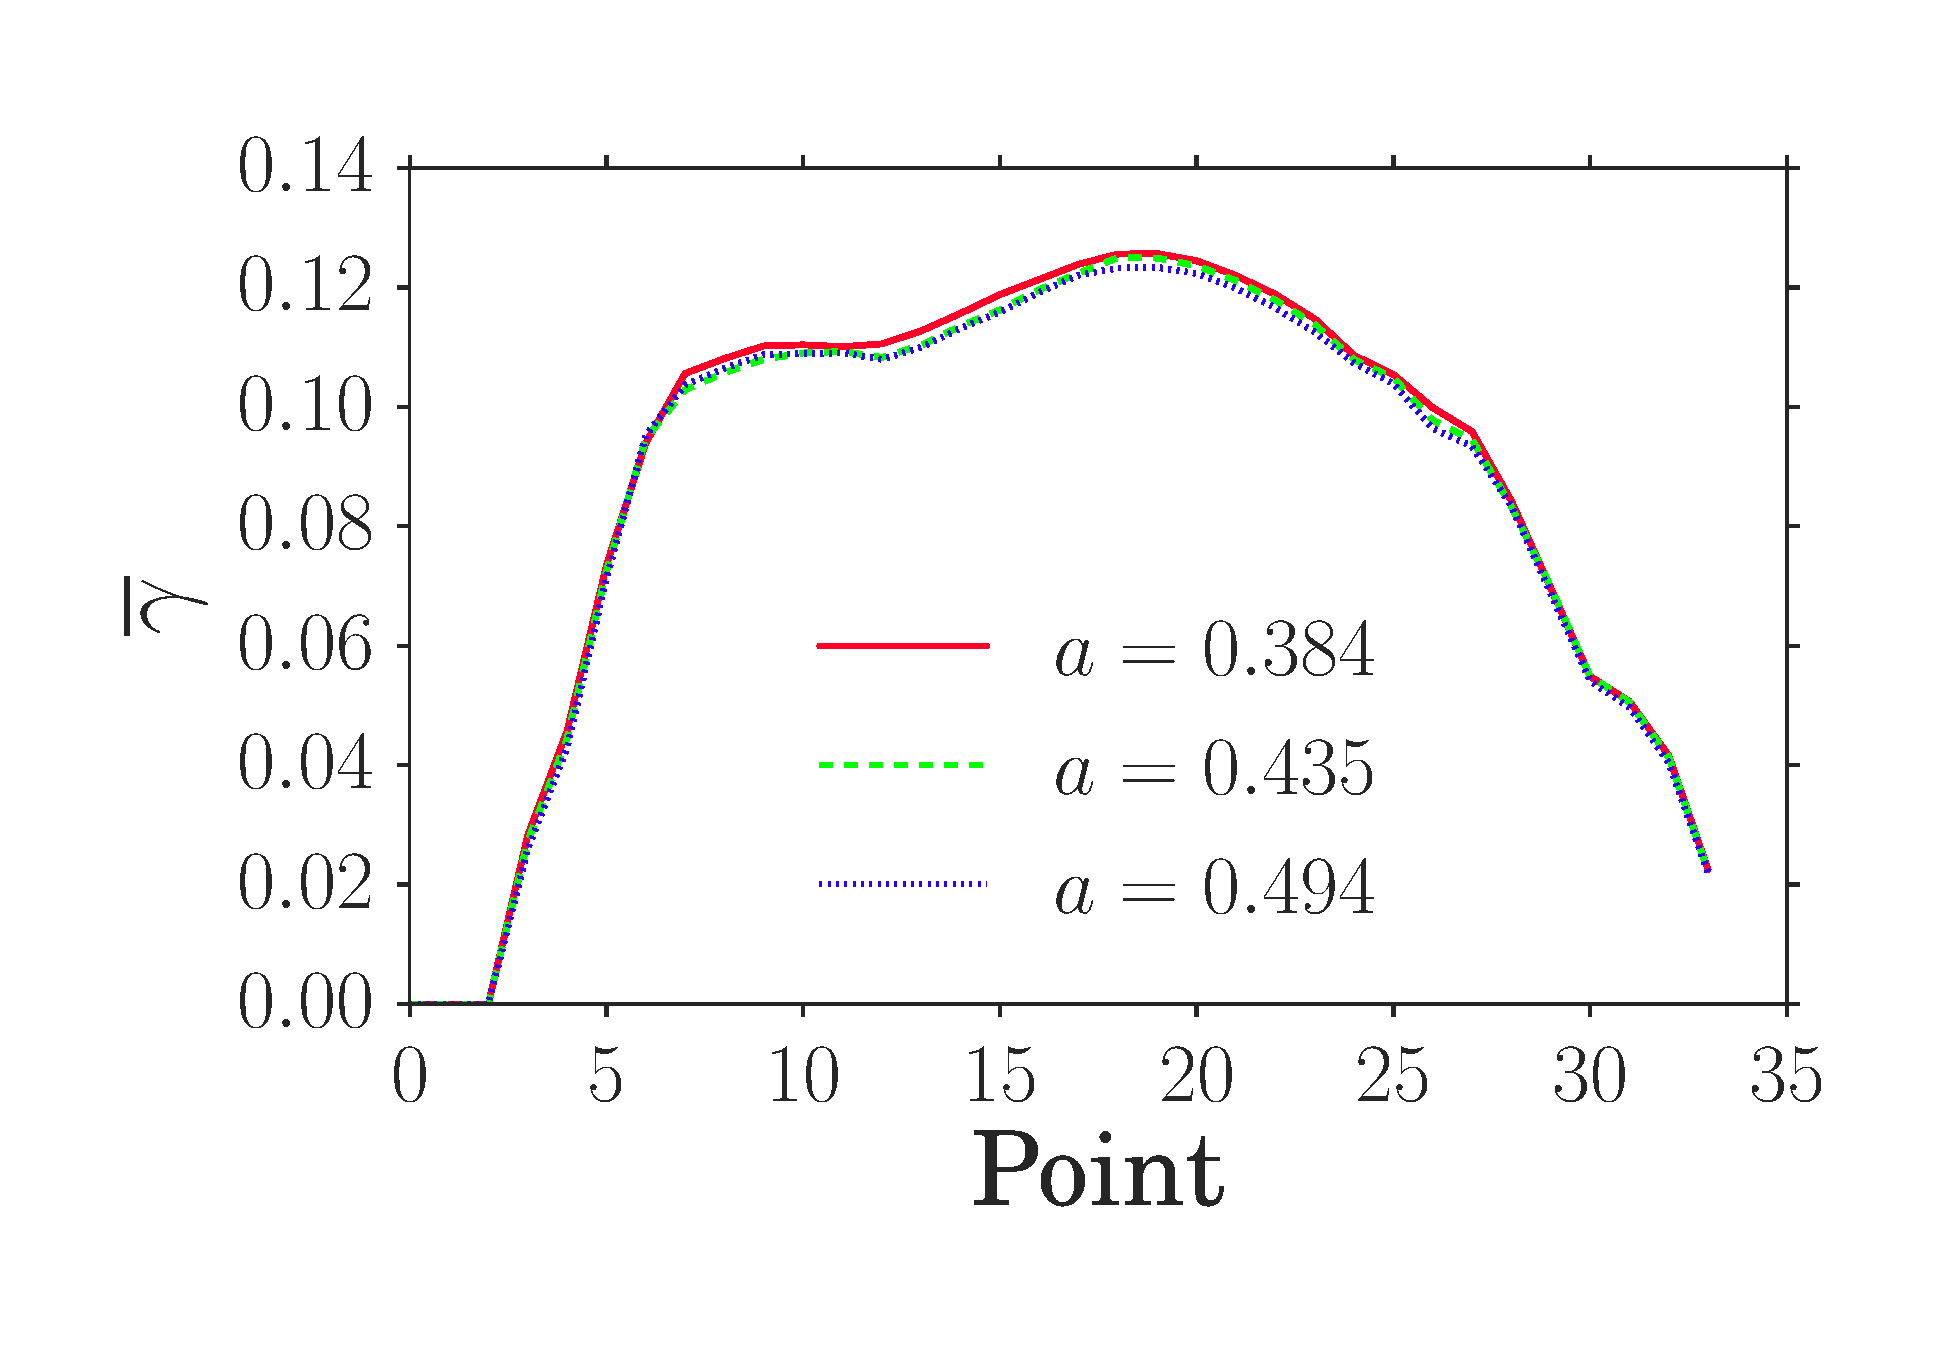
\includegraphics[width=0.7\textwidth]{mean_gamma_material_parameters_fixed}
\caption{Sensitivity of the optimal average contraction $\overline{\gamma}$ to changes in the parameter $a$. The upper and lower $a$
values are based on estimating $a$ with volume perturbations of $\pm 25 \% $ (Tabel~\ref{tab:passive_synth_opt}). The middle
 value was obtained by estimating $a$ from in-vivo volumes.}
\label{fig:gamma_sense_mat}
\end{figure}


\subsection{Sensitivity of estimated parameters to spring constant $k$.}
\label{sec:k_sense}
The spring boundary condition that we used at the ventricular base has a significant
effect on the simulated cavity volumes calculated by the model. This is due to the 
cross-sectional area of the cavity being large at the ventricular base. Therefore 
we can expect the choice of $k$ to have an effect on the optimal parameters calculated 
by our data assimilation. 

In order to quantify this effect we have
carried out a sensitivity analysis, starting with the effect of $k$ on the optimized elastic parameter $a$.
We repeated the elastic parameter fitting decribed in Section~\ref{sec:elasticparam} and varied the $k$-value from 0.001 to 100.0.
We also considered the case $k = \infty$, denoting a completely rigid boundary held by
Dirichlet boundary conditions. The effect of the choice of $k$ on the
optimal value of $a$ is shown in Table~\ref{tab:elast_sense}. The
table shows that the optimal $a$ varies from 0.365 kPa to 0.875 kPa depending upon how the $k$ parameter is set. 

We also tested the sensitivity of the contraction $\gamma$ at P1 resolution to $k$ by
repeating the estimation of $\gamma$ with the various $k$ and $a$ pairs obtained in the
previous experiment. For each $k, a$ pair we have plotted the spatial average of contraction $\overline{\gamma}$
at each measurement point in Figure~\ref{fig:gamma_sense}. The results
show up to a $20 \%$ variation in $\overline{\gamma}$ and
very little variation for the choices of $k$ greater than or equal to
1.0. For some of the values of $k < 1.0$ our homotopy Newton solver was unable to 
secure convergence during the optimization. Curves corresponding to
these cases are drawn only to the point before the non-convergence occurred.


\begin{table}
\caption{Sensitivity of optimal $a$ value to choice of spring constant $k$.}
\begin{tabular}{|l|llllllllllll|}
\hline
      $k$ & $10^{-8}$ & $10^{-7}$& $10^{-6}$&  $10^{-5}$  & $10^{-4}$ & $10^{-3}$ & 0.01 & 0.1 & 1 & 10 & 100 & $\infty$ \\
\hline
      $a$ & 0.875   & 0.875  & 0.875  & 0.875 & 0.873& 0.873 & 0.849 & 0.684 & 0.435 & 0.375& 0.366 & 0.365 \\
\hline
\end{tabular}
\label{tab:elast_sense}
\end{table}

\begin{figure}[t]
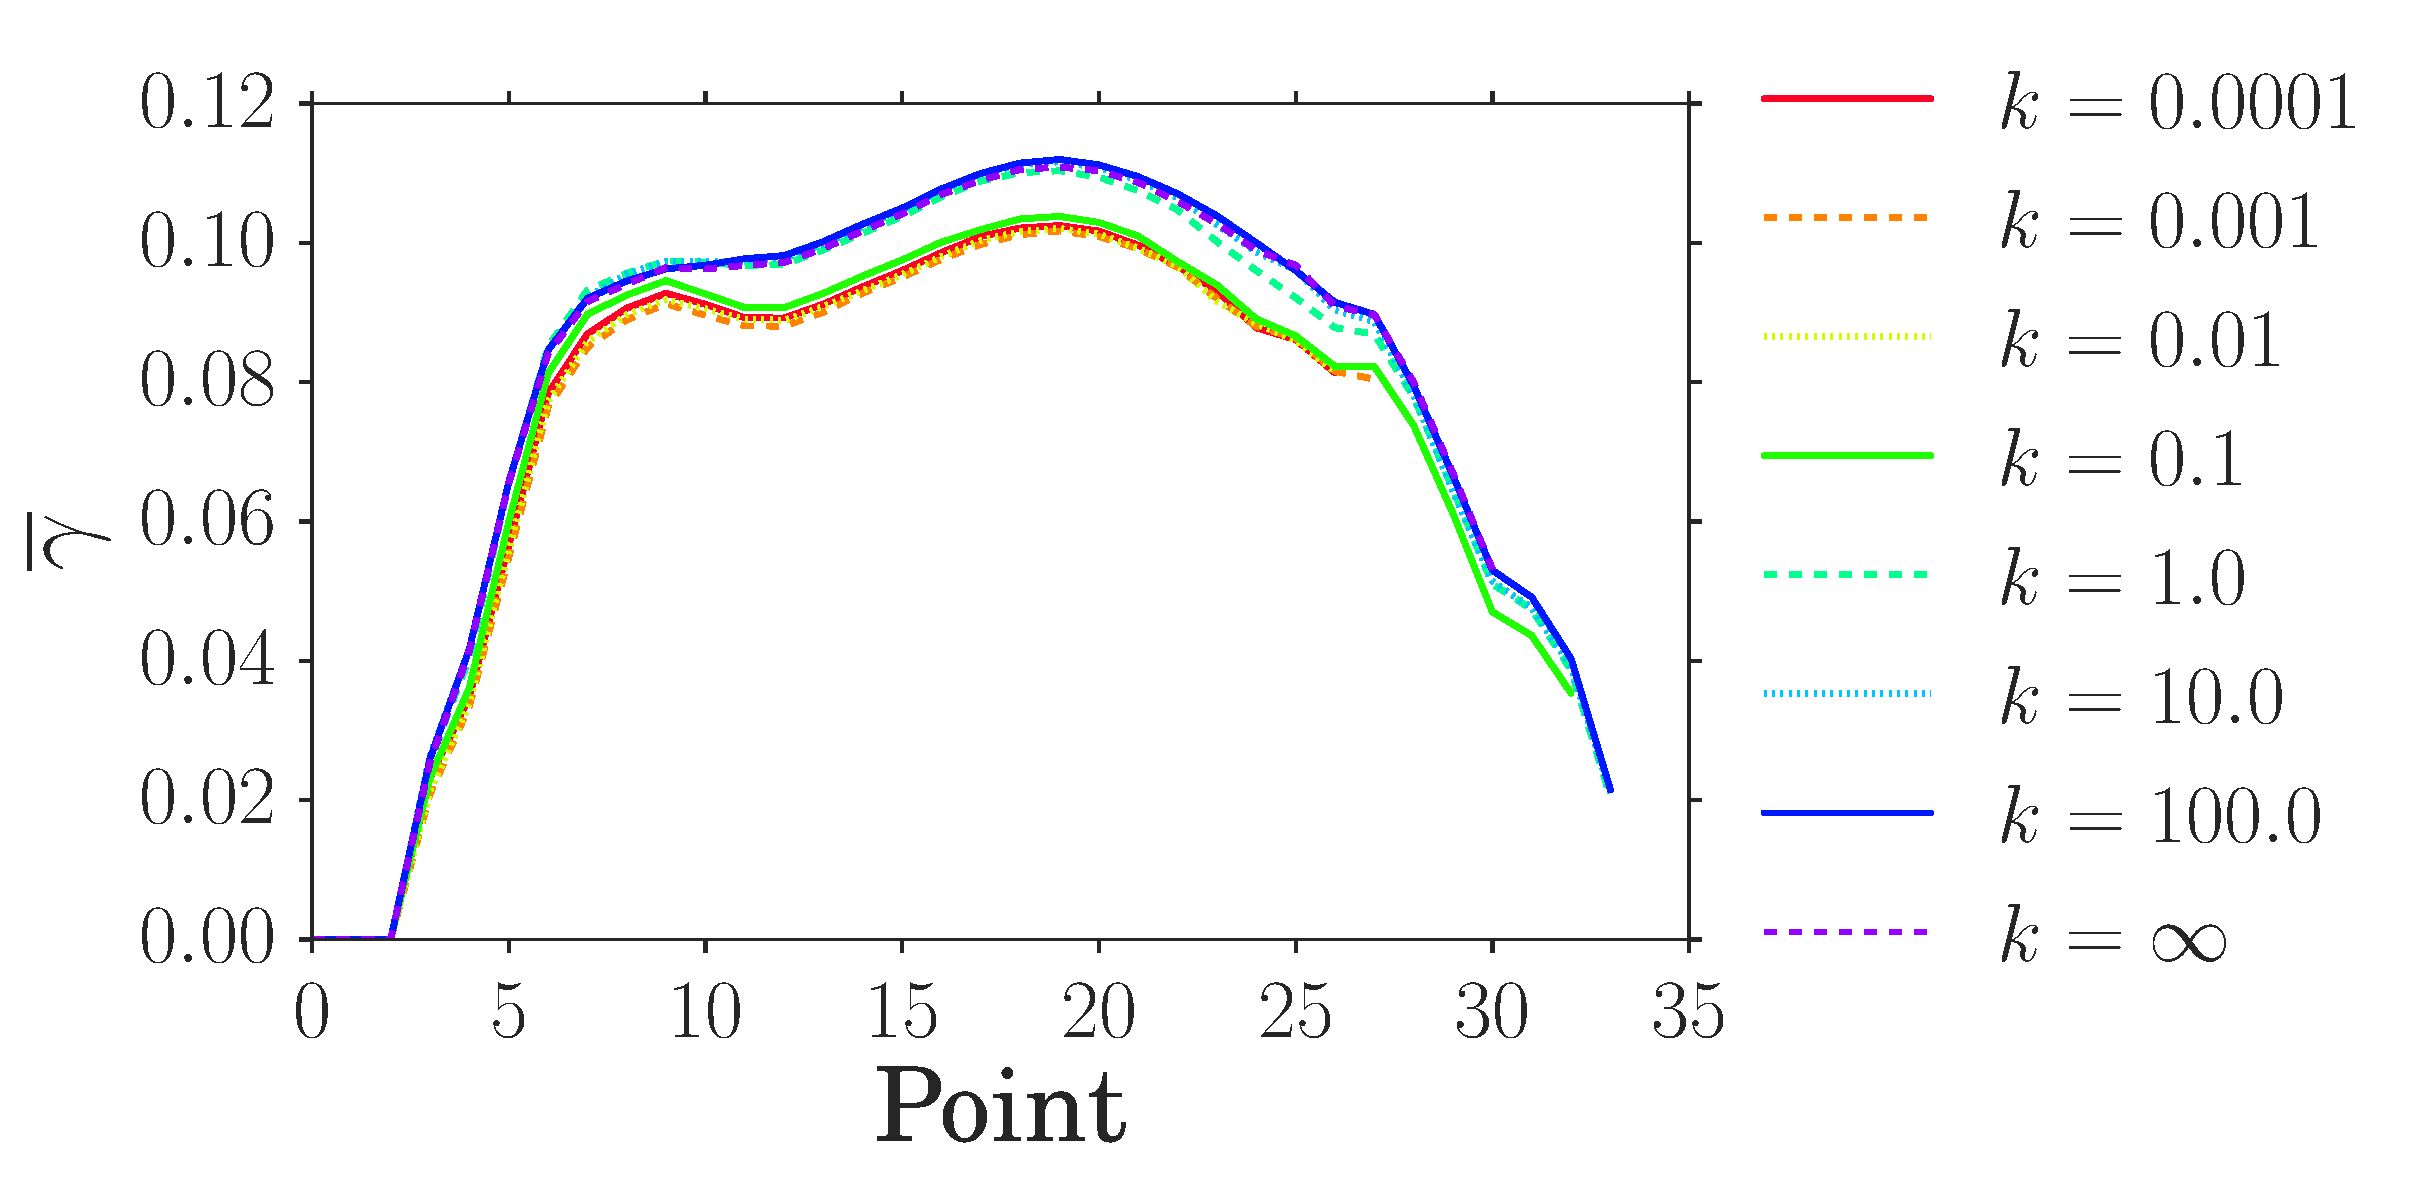
\includegraphics[width=0.7\textwidth]{gamma_mean}
\caption{Sensitivity of the spatially averaged 
contraction $\overline{\gamma}$ to the choice of spring constant $k$.}
\label{fig:gamma_sense}
\end{figure}


\subsection{Effect of mesh resolution on estimated contraction $\gamma$ at P1 resolution}
\label{sec:mesh_res}
Ventricular meshes were generated by Gmsh
\cite{geuzaine2009gmsh} with three different resolutions controlled by the parameter
'Mesh.CharacteristicLengthFactor'.  This parameter
was given the values $1.0$, $0.65$ and $0.45$ which resulted in meshes with
$549$, $1262$ and $2261$ vertices respectively. Using the three meshes
we estimated contraction fields from the in-vivo data. The average value of
$\gamma$ is shown for these three cases in Figure~\ref{fig:mesh_conv_gamma}. 
Fit quality is compared in Table~\ref{tab:mesh_conv_opt_misfit}.

\begin{table}
\caption{Relative misfit for different mesh resolutions}
\begin{tabular}{llll}
\toprule
Number of elements & $\Ivolavg$ & $\Istrainavg$ & $\Istrainrelmax$ \\ 
\midrule
549  & 0.0033 & 0.17 & 0.029 \\
1262 & 0.0037 & 0.17 & 0.029 \\
2661 & 0.0043 & 0.18 & 0.031 \\
\bottomrule	
\end{tabular}
\label{tab:mesh_conv_opt_misfit}
\end{table}

\begin{figure}[]
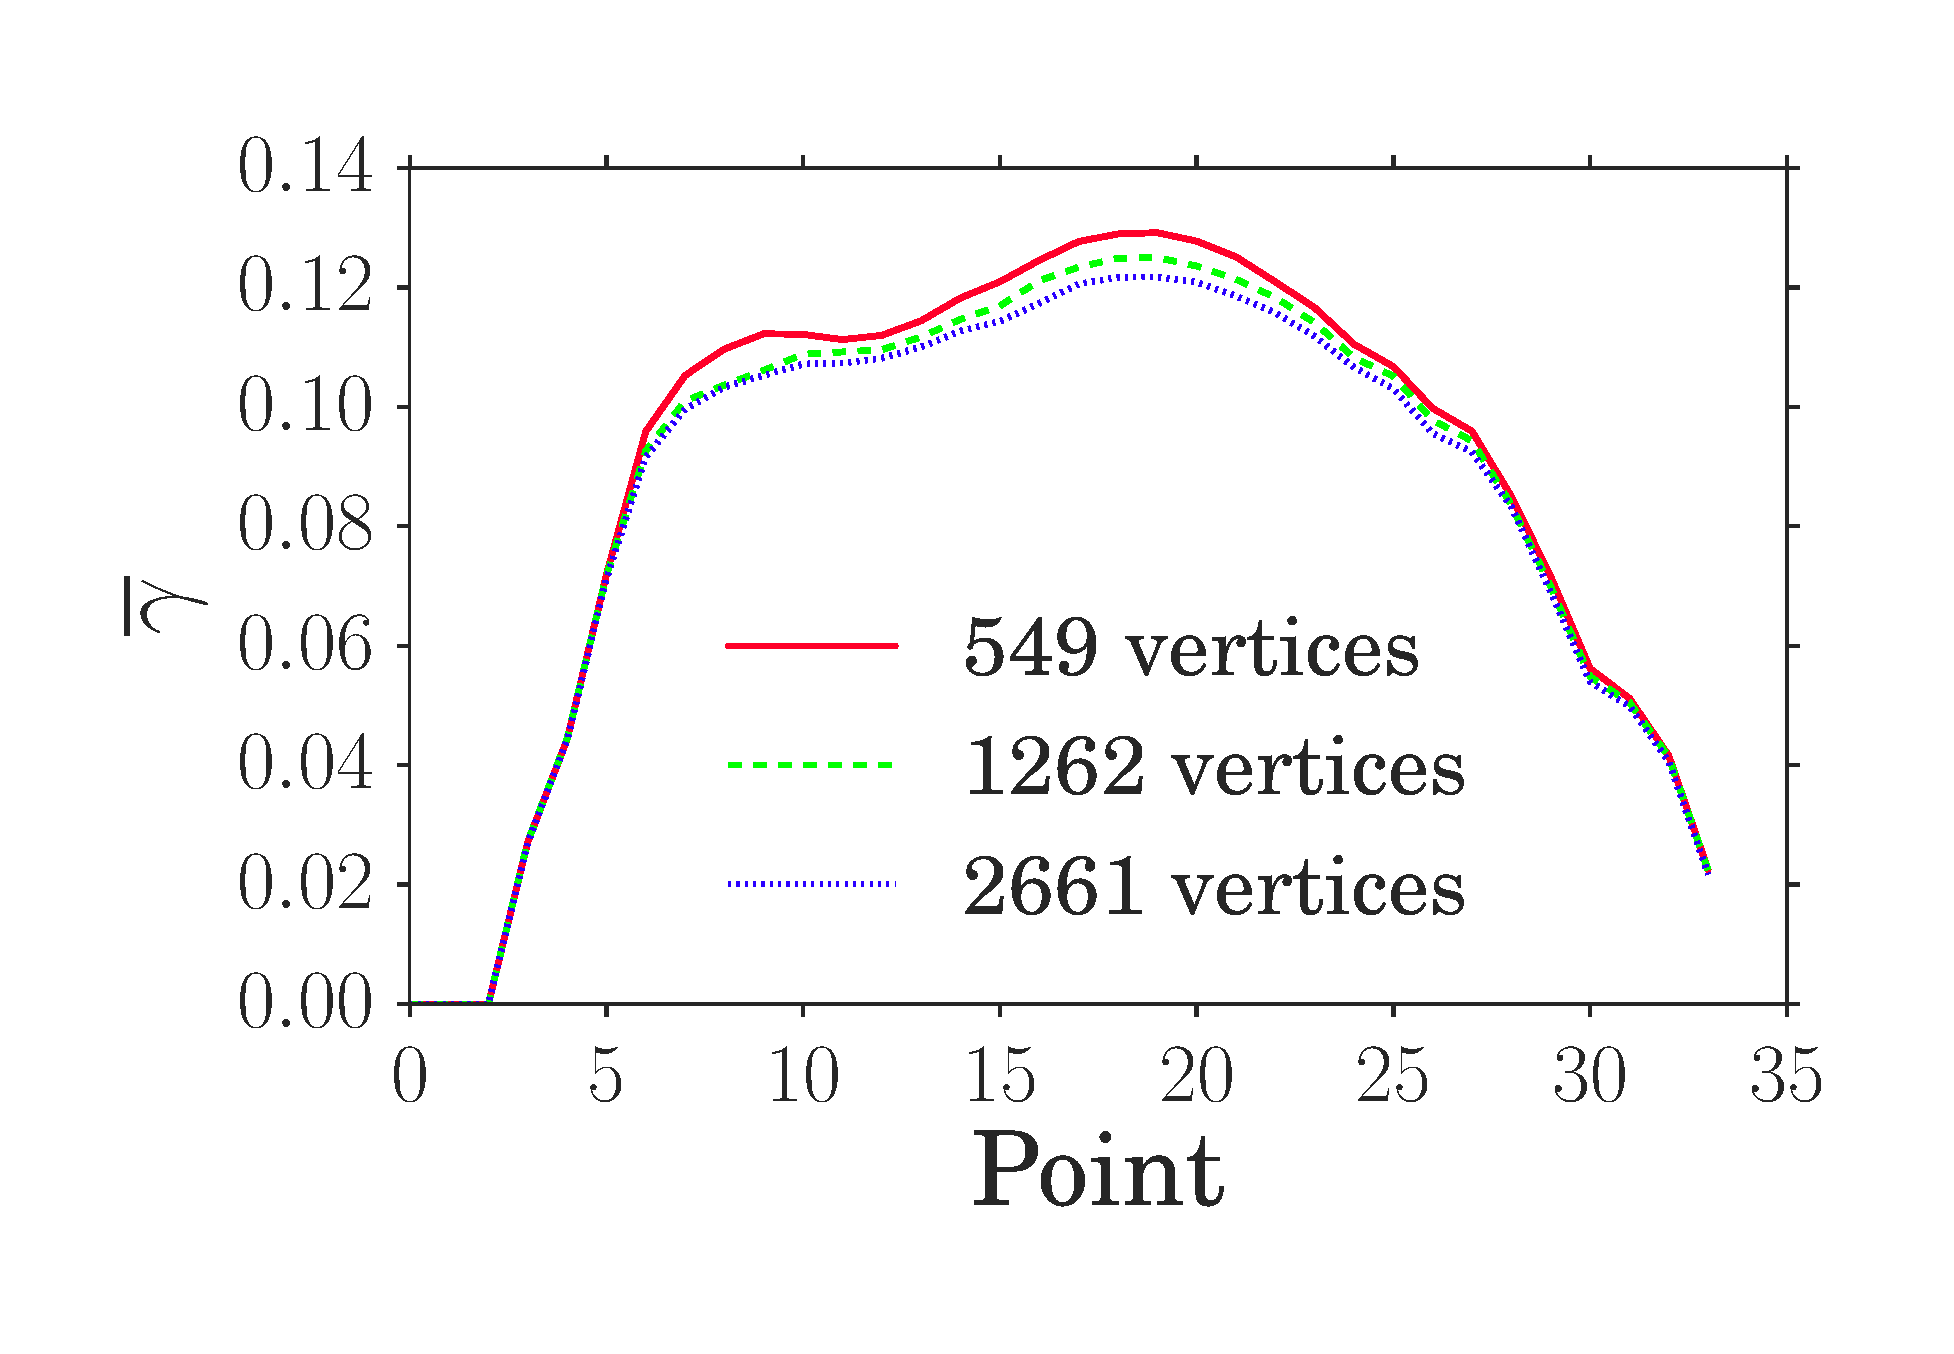
\includegraphics[width=0.6\textwidth]{mesh_conv_gamma}
\caption{Spatial average of contraction $\overline{\gamma}$ for 3 different mesh
  resolutions.}
\label{fig:mesh_conv_gamma}
\end{figure}


\subsection{Sensitivity of Contraction Size to choices of $\alpha$ and $\lambda$}
\label{sec:sense_alpha_lambda}
Based on the trade-off curves in Figure~\ref{fig:lcurves} we chose 
the optimization weights $\alpha = 0.95$ and $\lambda = 0.01$ for the personalization
of our wall motion model to the in-vivo data. In order to show the effect of these 
choices on the optimized contraction field $\gamma$ we have varied
the $\alpha$ and $\lambda$ values and plotted the spatial averages of the resulting
contraction fields. The results show that the amount of contraction tends to increase
proportionally to both $\alpha$ and $\lambda$ beyond the thresholds $\alpha = 0.5$ and
$\lambda = 0.001$. 

\begin{figure}[htbp]
\centering
\begin{subfigure}[t]{0.49\textwidth}
     {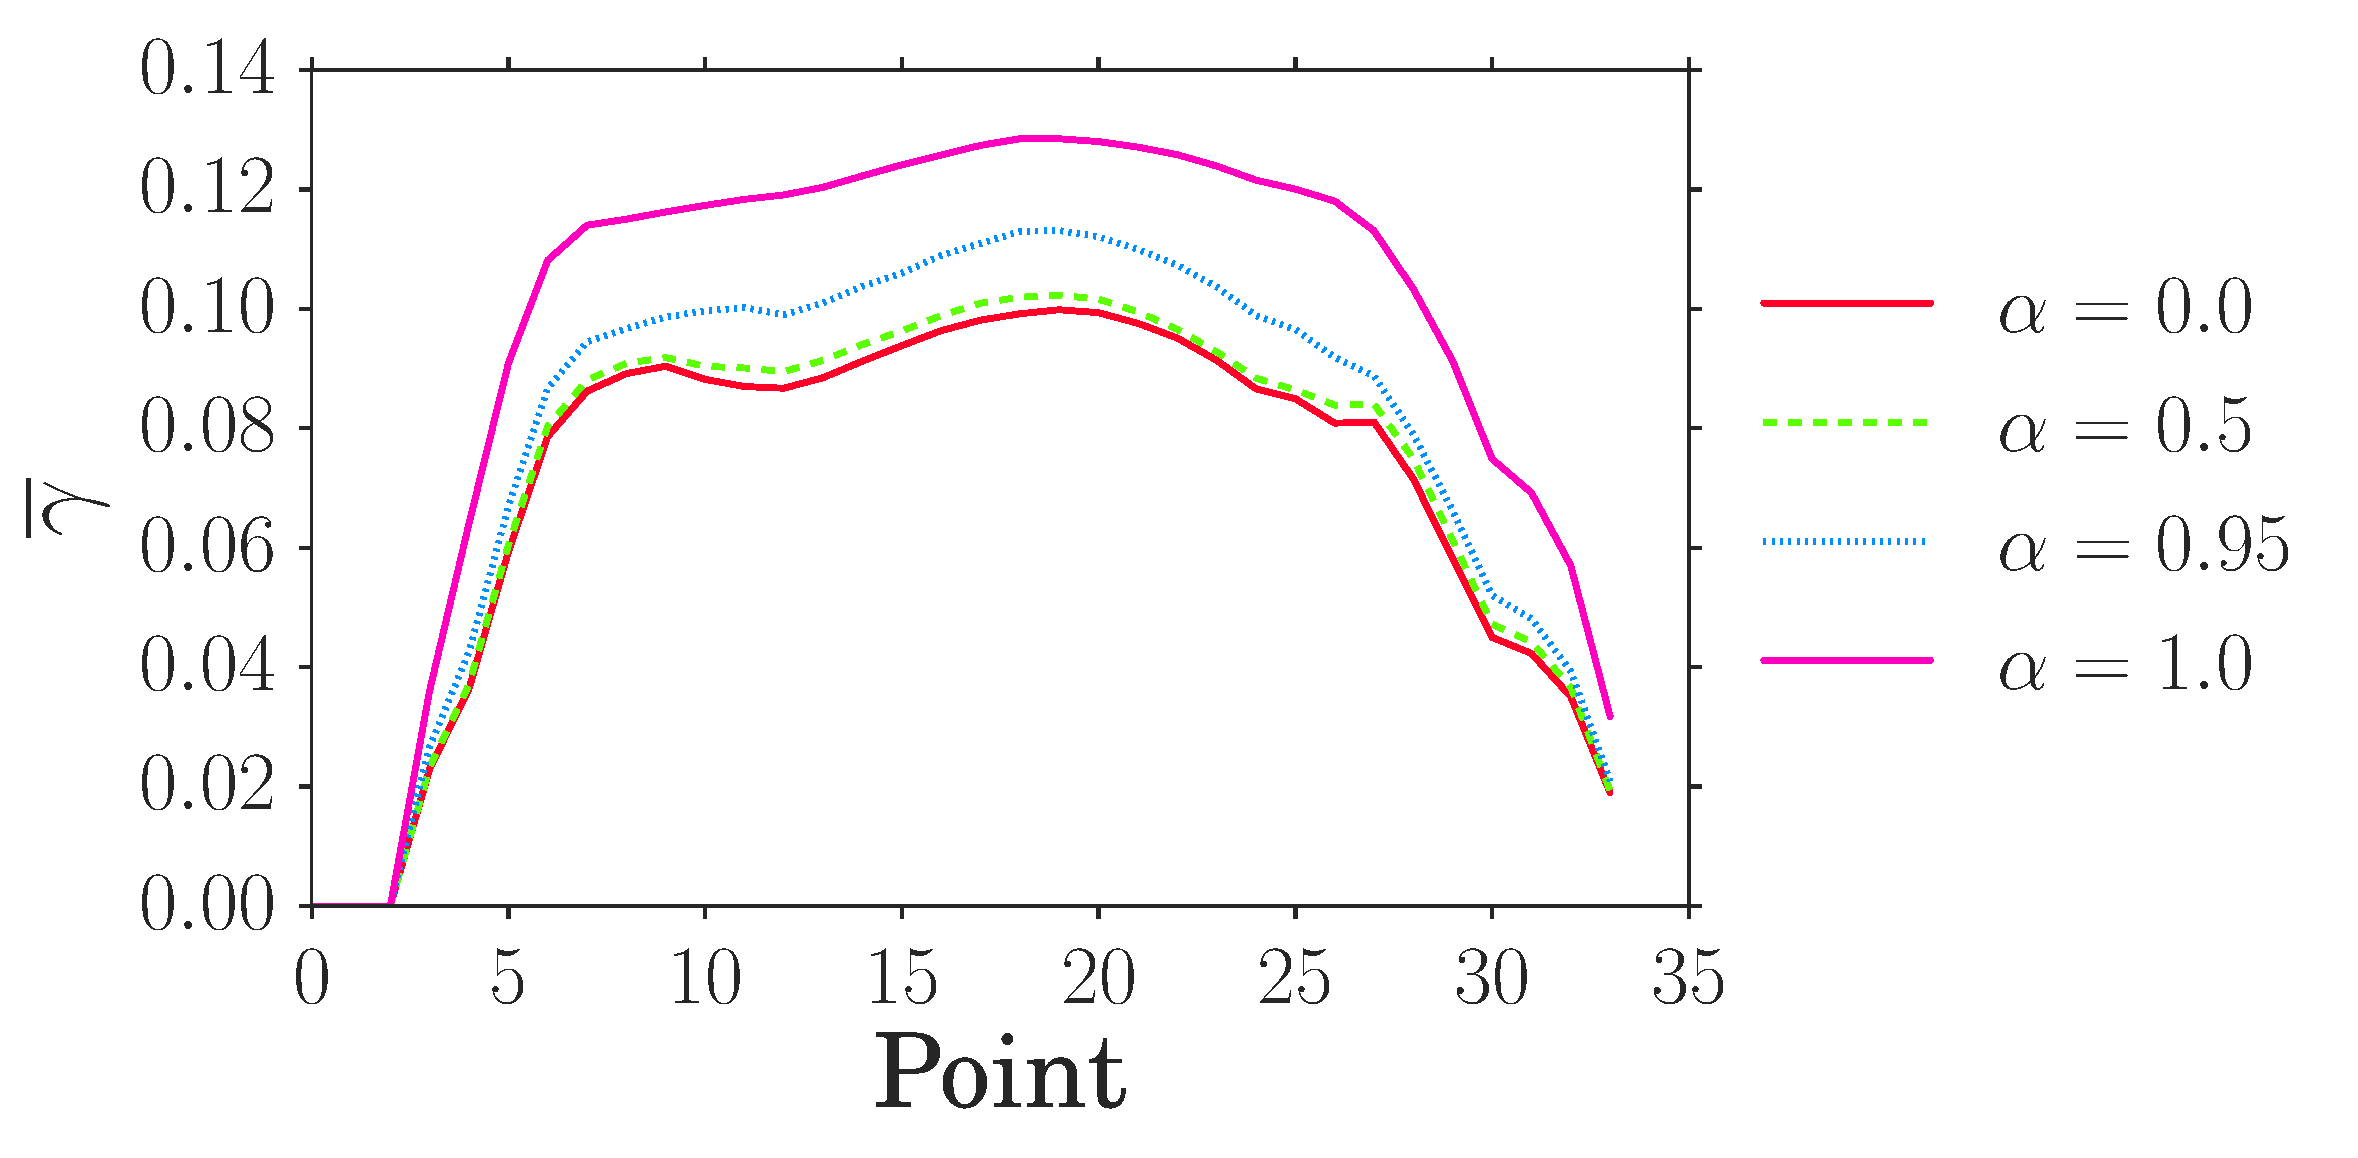
\includegraphics[width=\textwidth]{mean_gamma_varying_alpha}}
     \caption*{\label{fig:gamma_sense_alpha}}
\end{subfigure}
\begin{subfigure}[t]{0.49\textwidth}
    {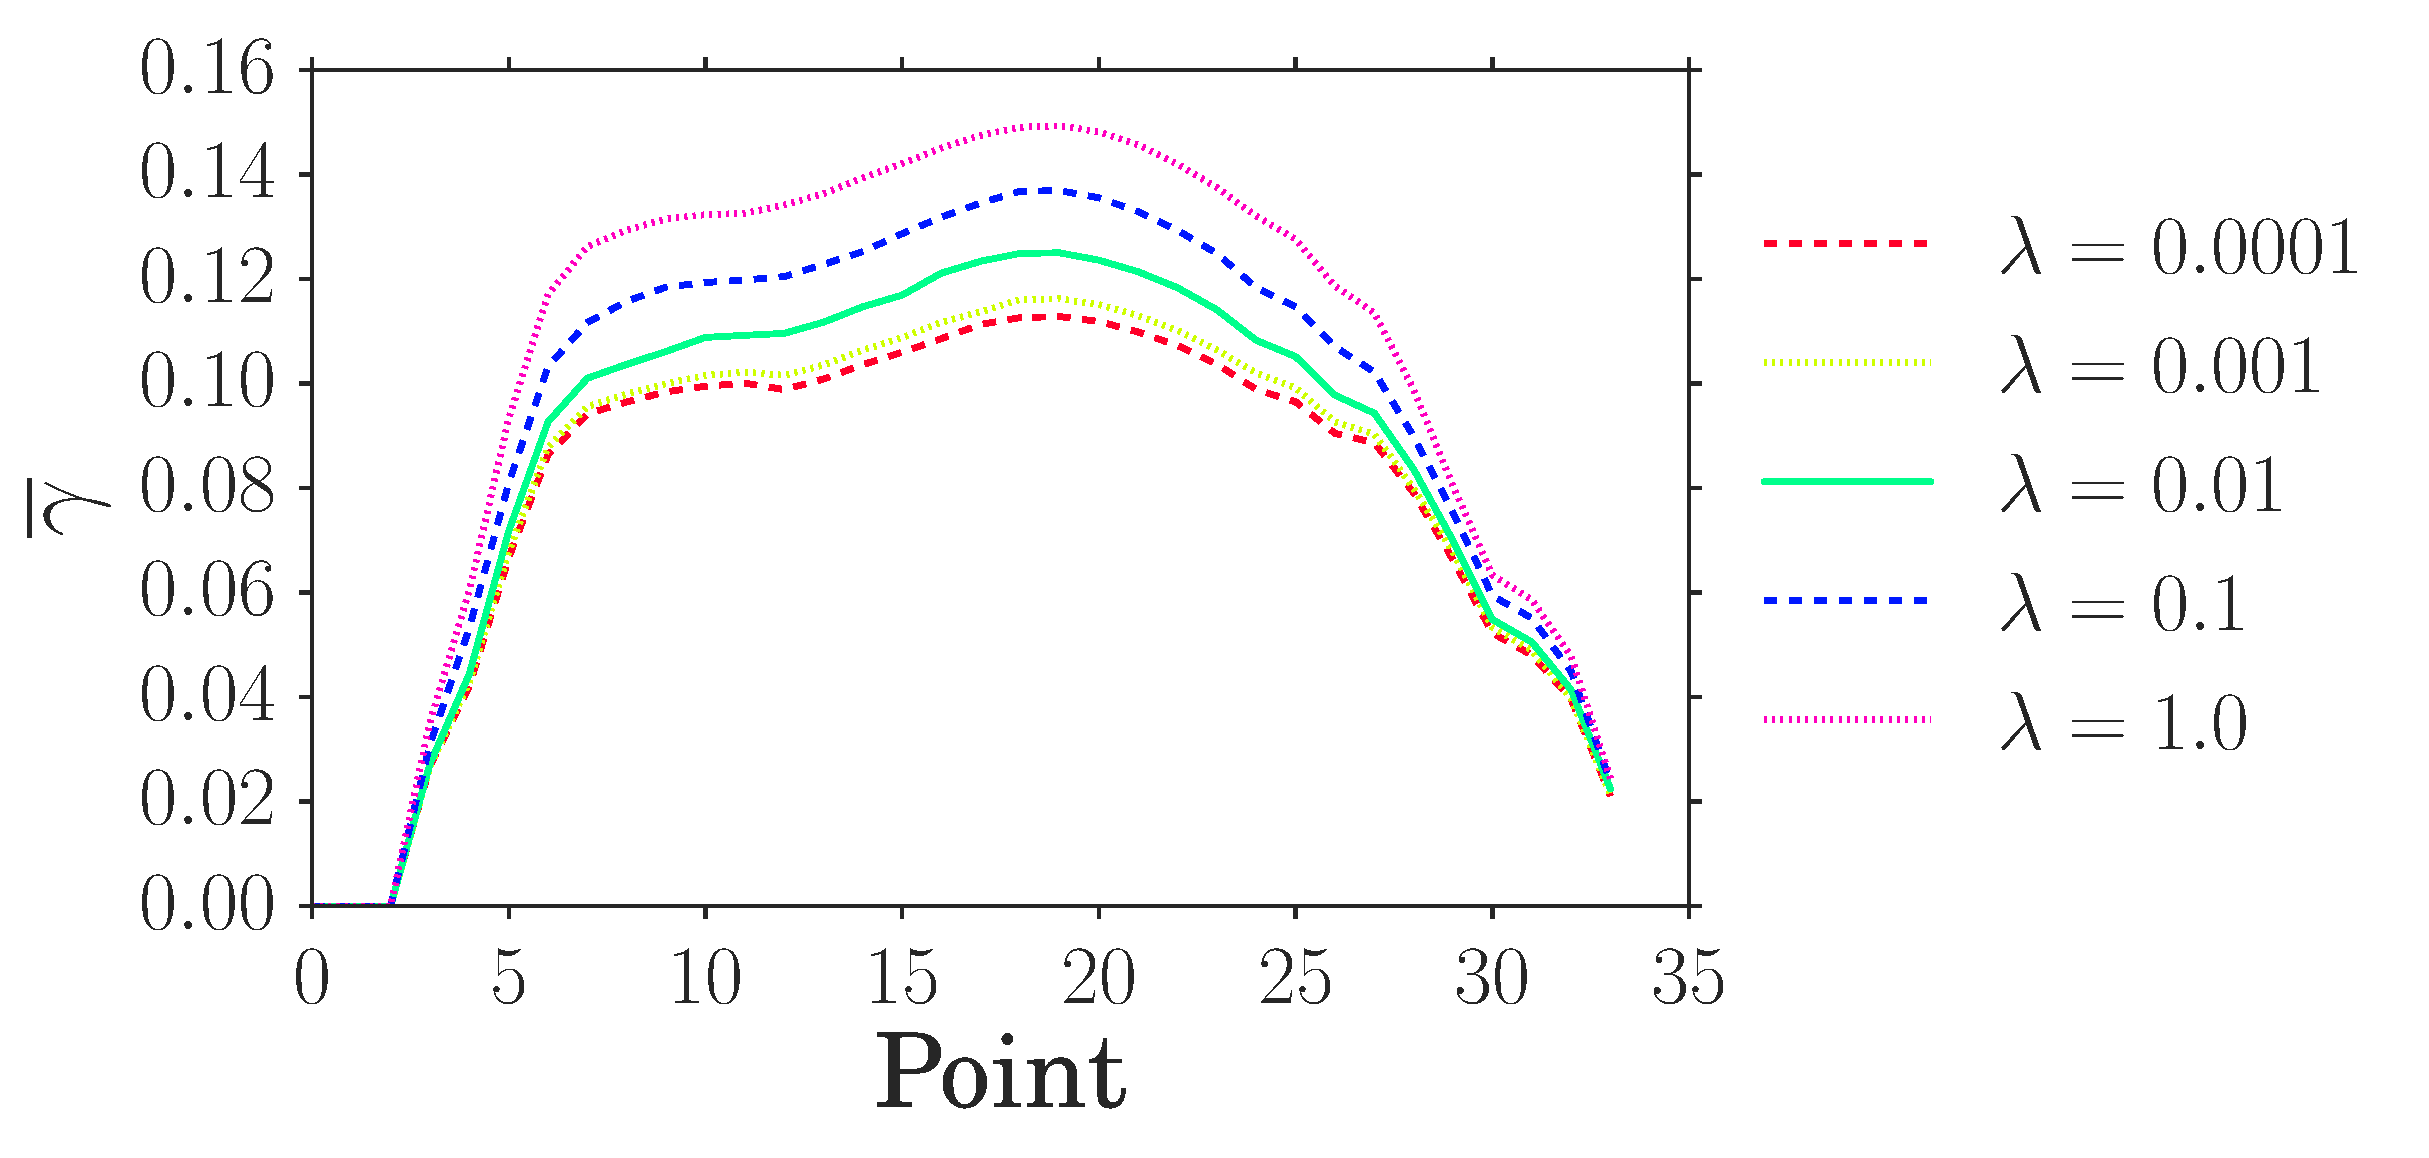
\includegraphics[width=\textwidth]{mean_gamma_varying_lambda}}
    \caption*{\label{fig:gamma_sense_lmbda}}
\end{subfigure}
\caption{Sensitivity of the spatially averaged contraction $\overline{\gamma}$ 
to variations in optimization weights $\alpha$ and $\lambda$. Left: $\lambda = 0$ and 
$\alpha$ is varied. Right: $\alpha = 0.95$ and $\lambda$ is varied.}
\label{fig:gamma_sense_alpha_lambda}
\end{figure}


\subsection{Estimation of noise in echo speckle tracking strain measurements}
\label{sec:strain_noise_est}
In order to increase the relevance of the synthetic tests we
considered a set of regional strains that contained noise. This
noise was modelled as an additive Gaussian process in order to imitate
the accumulation of tracking errors in EchoPac's image based strain
calculations. The mean and variance of a summand in the Gaussian
process were estimated from our in-vivo strain data of a single patient. From this data 
the sample means and variances of
the drift values were divided by the number of measurement points in order to approximate the noise in 
a single measurement. The mean and covariance of this single measurement point noise are given in
Table~\ref{tab:noise_covar_mean}.Theoretically, error free strain
curves would have no drift given stable conditions in the heart.
This motivates the use of the drift values in order to approximate 
the tracking error.

\begin{table}
  \caption{Mean and covariance of a Gaussian noise summand
    estimated from patient drift values in circumferential (C), radial
    (R) and longitudinal (L) directions.}
  \begin{center}
    \begin{tabular}{|l|ccc|c|}
      \hline
      & \multicolumn{3}{l|}{Covariance $\times 10^{-4}$} & Mean \\
      & C & R & L & \\
      \hline
      C &1.43 & 0.73 & 0.66  & 0.006 \\
      R& -    & 6.8 & 6.31  & -0.013 \\
      L &  -   &  -   & 7.26 & 0.01  \\
      \hline
    \end{tabular}
    \label{tab:noise_covar_mean}
  \end{center}
\end{table}




% \FloatBarrier
\pagebreak

\bibliographystyle{plain}
\bibliography{chapters/paper1/bibliography}

% \end{document}


%%% Local Variables:
%%% mode: latex
%%% TeX-master: "../../main"
%%% End:

 
\graphicspath{{chapters/paper2/figures/}}


\chapter{Paper 2: \\Estimating cardiac contraction through high resolution data
  assimilation of a personalized mechanical model}

% \clearpage
\newpage
\section*{Estimating cardiac contraction through high resolution data
  assimilation of a personalized mechanical model}

\begin{center}
  Henrik Finsberg
  Gabriel Balaban,
  Stian Ross,
  Trine H\r{a}land,
  Hans Henrik Odland, 
  Joakim Sundnes, and
  Samuel Wall
\end{center}

 
\subsection*{Abstract}
% \begin{abstract}
  
Cardiac computational models, individually personalized, can provide
clinicians with useful diagnostic information and aid in
treatment planning.  A major bottleneck in this process can be  
determining model parameters to fit created models to individual
patient data. However, adjoint-based data assimilation techniques can
now rapidly estimate high dimensional parameter sets.  This method is
used on a cohort of heart failure patients, capturing cardiac mechanical
information and comparing it with a healthy control group.  Excellent
fit ($R^2 \geq 0.95$) to systolic strains is obtained, and analysis
shows a significant difference in estimated contractility between the
two groups.


% \clearpage
\newpage
%% main text
\section{Introduction}
\label{sec:introduction}

Patient-specific cardiac modeling has emerged as a potential tool
for clinical diagnosis as well as treatment
 optimization\cite{viceconti2016virtual}.  By linking
patient measurements to physical processes through a mathematical
framework, models can provide us with additional insight into
cardiac function or dysfunction at the level of the
individual. However, the complexity of the heart makes this difficult,
and this is recognized as a key challenge in modern bioengineering
\cite{hunter2010vision}. 

One difficulty is the effort to personalize models and
simulations to individual patients.  While a wealth of clinical 
data exists to parameterize such 'patient-specific' models, methods to
assimilate this data into simulations can involve extensive
computation time, often putting them outside the scope of clinical
utility. However, new methods are emerging to improve the flow of clinical
measurements into powerful data driven simulations.  Automated
geometry segmentation \cite{rabben2010technical} and improved
optimization techniques \cite{chabiniok2012estimation}, can improve the
speed at which patient-specific models can be built and parameterized.
In particular, recent advancements in adjoint-based data assimilation
techniques \cite{balaban} offer an efficient way to assimilate ventricular mechanical
 information using highly spatially resolved parameters.  
 
Here we use an adjoint based assimilation method with a mechanical
model in order to construct simulations that 
accurately reflect clinical motion data, both for
healthy controls and patients suffering from left bundle
branch block (LBBB). The use of a highly spatially resolved
contraction parameter, enabled through adjoint-methods, provides
excellent data fit to measured strains and volumes, and fit models
provide estimates of cardiac contraction. Such biomarkers may prove
useful to clinicians for diagnoses of problems with cardiac function,
and to better plan therapies.    

\section{Materials and methods}
\label{sec:methods}

\subsection{Data acquisition}
\label{sec:clinical_data}

Clinical measurements of cardiac function for seven LBBB patients were
obtained from the Impact study \cite{ImpactStudy2016}.
Data was also acquired for seven healthy volunteers. 4D echocardiographic
images of the left ventricle (LV), for both the LBBB patients and
healthy subjects, were captured using
a GE Vingmed E9 device, and analysis carried out with the
software package EchoPac. For each subject, depending on frame rate and cardiac cycle time, the
analysis provided between 15 and 50 LV volumes,  geometric segmentations of the LV
endocardium and epicardium, and cardiac strain calculated via speckle
tracking. The strain were defined according to
the 17 segment AHA-zone representation
\cite{cerqueira2002standardized}, in the longitudinal, radial and
circumferential direction, giving a total of 51 strain measurements
per time point, with the reference time point for strain analysis
  being the first frame after onset of QRS.

The LBBB patients had LV pressure measurements taken during
implantation of a cardiac resynchronization therapy (CRT) device, and
valvular events were used to synchronize the pressure to the echo
data. In the healthy control group, where invasive pressure measurements were
absent, the pressure waveform from one of the LBBB patients was used and
scaled to reported values of the end-diastolic and end-systolic
left ventricular pressure [Table 30-1 in \cite{klingensmith2008washington}].


\subsection{Automated geometry and microstructure creation}
For each patient, a 3D tetrahedral mesh of the LV was
constructed from triangulated segmented surfaces of the endo- and
epicardium corresponding to the frame at the beginning of
atrial systole, Figure \ref{fig:pipeline}. A cut was made at the
ventricular base of the segmentation, so that the mesh cavity volume
and the ultrasound measured volume differed by less than  $1$ ml. Mesh
cells were marked into the 17 AHA regions through the regionally
delineated strain data, and the myocardial fiber orientation, denoted
by $\ef$, were assigned using the algorithm from Bayer et al \cite{bayer2012novel},
with the endo- and epicardial helix fiber angles set to
$\alpha_{\text{endo}} = 60$ and $\alpha_{\text{epi}} = -60$, respectively.

\subsection{Mechanical Model}
We represent the heart as a hyperelastic continuum body, where the coordinates in
the reference ($\Xvec$) and the current ($\xvec$) configuration are
related via the displacement field $\uvec = \xvec-\Xvec$. Furthermore,
we utilize the
deformation gradient, the determinant of the deformation gradient
and, the right Cauchy-Green deformation tensor given by $\F= \I+\nabla
\uvec $,  $J = \det \F$ and $\C = \F^T\F$, respectively. 
% Constitutive relations
To model the passive behavior of the myocardium, the transversely 
isotropic strain energy function proposed in  \cite{holzapfel2009constitutive} is adopted:
\begin{align}
\label{eq:hoa}
  \mathcal{W}(I_1, I_{4\ef}) = \frac{a}{2 b} \left( \exp\left\{ b (I_1 
  - 3)\right\}  -1 \right)
  + \frac{a_f}{2 b_f} \left( \exp\left\{ b_f (I_{4\ef} 
  - 1)_+^2\right\} -1 \right).
\end{align}
Here $I_1 = \tr \C$ and $I_{4\ef}= \ef \cdot (\C \ef)$ are invariants
of $\C$, $(\cdotp)_{+}  = \max\{\cdot, 0\}$, and $a, a_f, b, b_f$ are
material stiffness parameters defining the elastic properties of the myocardium.
% Incompressibility
We follow a common approach and assume that the myocardium is incompressible. 
Incompressibility is incorporated in the model by using a two-field variational 
approach, where we introduce a Lagrange multiplier $p$ which represents the 
hydrostatic pressure, and the term $p(J-1)$ is added to the strain-energy.

% Active response
To model the active response we apply the approach of active strain
\cite{ambrosi2012active}, which is based on decomposing
the deformation gradient into active and passive contributions, $\F =
\F_e \F_a$. We choose $\F_a = (1 - \gamma) \ef \otimes \ef +
\frac{1}{\sqrt{1 - \gamma}} (\I - \ef \otimes \ef)$, where $\gamma$
is a parameter that represents the relative active shortening along
the fibers. For reference, we have also performed tests with the
commonly used active stress formulation, where the stress tensor 
is additively decomposed into active and passive stress $\sigma =
\sigma_p + \sigma_a$. Here $\sigma_p$ is
the elastic material response, and $\sigma_a = T_a \Fef \otimes \Fef$ with
$\Fef = \F\ef$ and $T_a$ a scalar variable representing active fiber
tension.


For both approaches, the resulting displacement field $\uvec$ and hydrostatic pressure $p$
are determined by using the principle of stationary potential energy
\cite{holzapfel2000nonlinear}, which is based on minimizing the total
energy  $\Pi(\uvec, p)$, which includes internal energy derived from
\eqref{eq:hoa} and external energy. The external energy includes
contributions from the measured cavity pressure $p_{\text{LV}}$, and a
linear spring term at the basal boundary, with spring constant
$k$ = 10.0 kPa. The equilibrium solution is found by solving for the minimum
potential energy, $\delta\Pi(\uvec, p) = 0$. 

\subsection{Data Assimilation}
In order to constrain the model to each patient's clinical measurements, we
consider a PDE-constrained optimization problem where
the objective functional is given by the misfit between
simulated and measured strain and volume along with a first order Tikhonov regularization of the
model parameters.
\begin{equation}
  \begin{aligned}
    \label{eq:pde_opt}
    & \underset{m}{\text{minimize}}
    & &  \alpha \left( \frac{V^i - \tilde{V}^i}{V^i} \right)^2
    + (1-\alpha)  \sum_{j= 1}^{17} \sum_{k \in \{c,r,l\}}  \left( \varepsilon_{kj}^i
      -  \tilde{\varepsilon}_{kj}^i \right)^2
    + \lambda \| \nabla m^i \|^2 \\
    & \text{subject to}
    & & \delta \Pi(\uvec, p) = 0.
  \end{aligned}
\end{equation}


Here $V$ and $\varepsilon_{kj}$ are the measured volume and regional Lagrangian strain in
segment $j$ in direction $k$ respectively, and $\tilde{V}^i =
-\frac{1}{3} \int_{\partial \Omega_{\text{endo}}} (\Xvec + \uvec)
\cdotp J\F^{-T}\Nvec  \mathrm{d}S$,  and $\varepsilon_{kj} =
\frac{1}{|\Omega_j|}\int_{\Omega_j}  \mathbf{e}_k^T \nabla \uvec \,
\mathbf{e}_k  \mathrm{d}x.$ 
The parameters $\alpha$ and $\lambda$
control the weights on the different terms, and the sum in the second
term is taken over the seventeen AHA
segments, and the three different strain components (Section \ref{sec:clinical_data}).


The data assimilation procedure is divided into two phases; a passive
and an active phase. For the passive phase we iteratively
  estimate the unloaded configuration and the linear isotropic parameter, $a$ in
\eqref{eq:hoa}, using an algorithm similar to the one described in
\cite{nikou2016effects}, and we set $\alpha= 1.0$,  with $\lambda = 0$ and
$\gamma = 0$, minimizing only the misfit with the measured volumes. The
remaining material parameters are fixed according to [Table 1 row 3 of
\cite{holzapfel2009constitutive}]. For the active phase we fix the material parameter optimized in the
passive phase, choose the control variable $m$ to be $\gamma$ or
$T_a$ for the active strain and active stress model respectively, and
set $\alpha = 0.95$ and $\lambda = 0.01$. This choice of $\alpha$ and
$\lambda$ was based on the analysis done in \cite{balaban}. A summary
of our optimization pipeline is provided to the right in
Figure~\ref{fig:pipeline}.





\begin{figure}[htbp]
\centering
    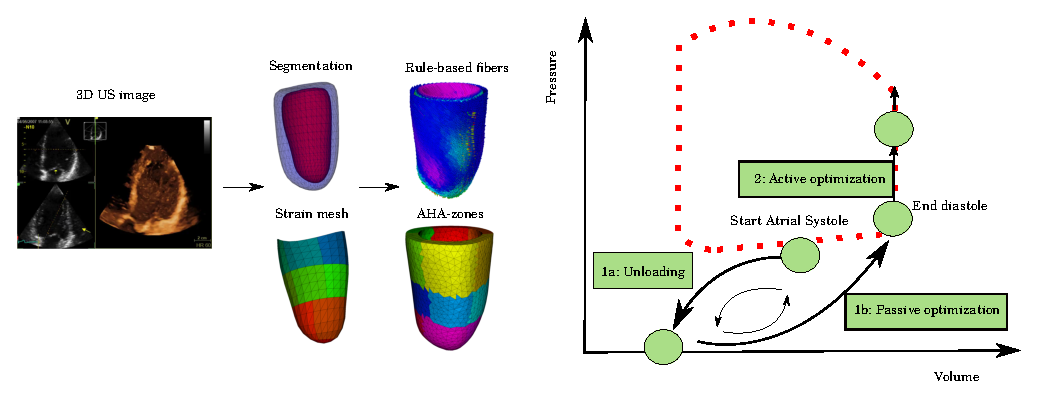
\includegraphics[width=\textwidth]{models}
\caption{Left: Automated anatomical modeling pipeline to produce AHA
  marked simulation meshes with applied fiber orientations from 3D
  echocardiographic segmentations. Right: Optimization
  pipeline. 1. Unloaded geometry and the linear isotropic
  material parameter $a$ in \eqref{eq:hoa} are estimated iteratively. The unloaded geometry is
  estimated based on the backward displacement method (1a)
  \cite{nikou2016effects} and $a$ is estimated by minimizing the
  difference between simulated and measured volumes (1b). 2. The unloaded
  geometry and the material properties are fixed, and the amount of
  contraction ($\gamma$ for active strain and $T_a$ for active stress)
  is estimated by minimizing the mismatch between simulated and
  measured strain and volume. The active optimization continues to the
  next measurement point until all measurement points in the cycle are covered.}
\label{fig:pipeline}
\end{figure}

\subsection{Implementation details}
We employ a Galerkin finite element method with Taylor-Hood
tetrahedral elements, that is $(\uvec, p) \in \mathbb{P}_2 \times
\mathbb{P}_1 $, with $\mathbb{P}_n$ being the space of piecewise
polynomials of degree $n$.
The solver is implemented in the finite element framework FEniCS
\cite{logg2012automated}, and uses a Newton trust region algorithm
\cite{PETScPackage} to solve nonlinear systems. The minimization of the
model-data misfit functional~\eqref{eq:pde_opt} is accomplished by a sequential
quadratic programming algorithm (SQP)~\cite{kraft1988software}, where
the functional gradient is computed by solving an automatically derived adjoint
equation \cite{farrell2013automated}. In these minimizations an upper
bound of $0.5$ and $500$ kPa is set for the active strain ($\gamma$)
and active stress ($T_a$) control variable respectively, which both
are modeled as functions in $\mathbb{P}_1$, yielding one parameter per
nodal point in the mesh.

\subsection{Contraction analysis}
Although direct physical interpretation of the active
  strain parameter $\gamma$ is difficult, it may be seen as the
  relative shortening of an isolated and unloaded muscle cell. A high
  value of $\gamma$ is therefore an indication of higher contractile
  force in the myocardium, independent of load. We propose that
  the spatially averaged $\gamma$ over the entire LV, denoted by  
  $\overline{\gamma}$, can be used as an index of global
  contractility. Similarly, the active stress parameter $T_a$ is related to force
  development at level of the sarcomeres\cite{goktepe2014generalized},
  and the spatially averaged 
  $T_a$, denoted $\overline{T_a}$ can be used as an index of
  contractility. In addition to the contractility information contained in 
$\overline{\gamma}$ and $\overline{T_a}$, the overall elastic state
of the optimized patient models 
can be used to give estimates of LV elastance. The left ventricular
end-systolic elastance $E\es$, the response of end systolic volume to
increased load, is considered to be one of the major determinants for
cardiac systolic function, and was in \cite{sagawa1977end} proposed
as a global index of ventricular contractility.
It is possible to estimate the end systolic elastance directly 
if the end systolic pressure is known or estimated, 
by perturbing the loading conditions on the optimized model at end
systole while fixing the remaining quatities, and calculating the slope
in the resulting ES pressure-volume curve. More
precisely, if $\plv^{\text{ES}}$ is the end-systolic ventricular
pressure, with cavity volume $V^{\text{ES}}$, 
we change the pressure to $\plv^{\text{ES} + \Delta} =
\plv^{\text{ES}} + \Delta \plv$, resulting in a change in volume,
$V^{\text{ES} +\Delta} = V^{\text{ES}} + \Delta V$. The estimate of end-systolic
elastance can then be calculated by 
\begin{align}
  \tilde{E}\es = \frac{\Delta \plv}{\Delta V}.
  \label{eq:estimate_elastance}
\end{align}



\section{Results and discussion}
\label{sec:results}


\subsection{Matching of strain and volume}
We show the results from two representative simulations in
Figure~\ref{fig:generic_result}, one from the LBBB group and one from
the healthy control group. Snapshots from the calculated unloaded and
end-systolic configurations are depicted. For the unloaded
geometry, we also show the image-based geometry at beginning of atrial
systole, and for the end-systolic configuration we show the
longitudinal strain using both the active stress and active strain
approach. We also show the agreement with the corresponding PV-loops.
% and one of the 51 strain traces over the cardiac cycle shown.  


\begin{figure}[htbp]
  \centering
  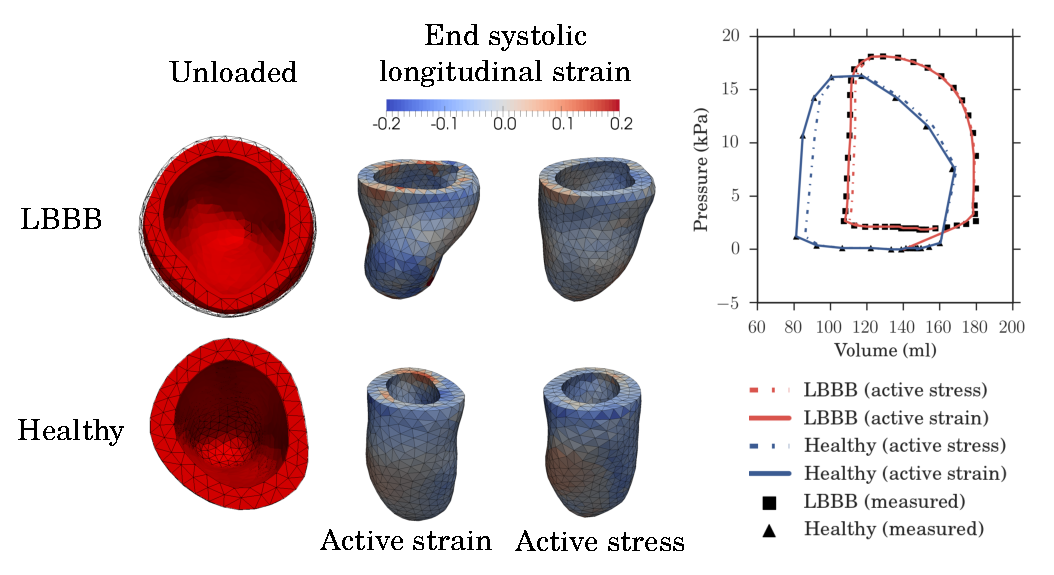
\includegraphics[width=\textwidth]{generic_result}
  \caption{Left: Snap shots of the unloaded geometry in red, and the
    corresponding image based geometry taken at beginning of atrial
    systole in black wire-frame. Middle: Snap shot of end systolic
    configurations using the active strain and active stress approach.
    Color-map shows the end-systolic longitudinal strain.
    Right: Simulated and measured pressure-volume loops for
    these hearts using the active strain and active stress approach.}  
  \label{fig:generic_result}
\end{figure}


The total analysis of the 14 patients involved optimizing 432 volume
measurements and 20 853 strain measurements. The average time for one
forward and gradient evaluation was 8.3 and 8.9 seconds respectively
when running on a cluster using four cores, with an average number of
control parameters being 985.

In order to visualize the overall match of simulated to measured data,
we show linear regression plots in
Figure~\ref{fig:data_matching}. These results are all based on the
active strain formulation. For
the strain, we separately consider the diastolic and systolic points,
as different types of data were used to  constrain the model in these
two phases, namely volume in the diastolic phase and strain in the
systolic phase. An excellent overall fit was obtained for the optimized
volume ($R^2=1.00$) and systolic strains ($R^2=0.95$). 
Diastolic strains, not used in the optimization, were less well
matched ($R^2=0.31$).



\begin{figure}[htbp]
  \centering
  \includegraphics[width=\textwidth]{data_matching}
  \caption{Scatter plot of simulated ($y$-axis) and measured
    ($x$-axis) strain and volume using the active
    strain approach. Left: Scatter plot of simulated versus
    measured volumes and the best linear least-squares fit of these
    points, (slope = $1.00$). Right: Scatter plot of simulated versus
    measured strain for all segments and all directions, separated
    into the diastole, were only the volume was optimized and systole,
    where both the strain and volume were optimized. For diastole, the slope of
    the best linear fit was $0.31$, while the best linear fit for the
    systolic points had a slope of $0.95$.}
  \label{fig:data_matching}
\end{figure}


\subsection{Estimation of global contractility and elastance}

Global contraction time courses, $\overline{\gamma}$ and
  $\overline{T}_a$, for each patient were synchronized to the valvular
events to normalize for differing cycle lengths. The average 
and standard deviation of these normalized traces for the
LBBB vs the healthy controls are shown in left of
Figure~\ref{fig:contractility}. The healthy patients had a much higher
level of contraction through the cardiac cycle, and the peak values
were compared using one-way ANOVA, yielding a $P-$value less than
$0.001$ for both the active strain and the active stress approach. 

The values of calculated $\tilde{E}\es$ for the healthy and LBBB patients are
shown to the right in Figure~\ref{fig:contractility}. The calculated
elastances of the LBBB group were significantly lower than for the healthy
group, with the comparison between the groups using one-way ANOVA
giving a $P-$value of $0.009$ and $0.003$ for the active strain and
active stress respectively.




\begin{figure}[htbp]
  \centering
  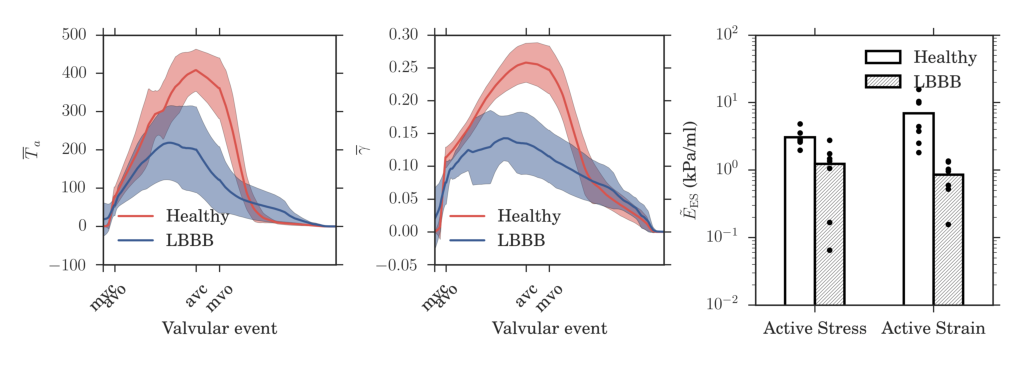
\includegraphics[width=\textwidth]{contractility}
  \caption{Extracted biomarkers related to cardiac contractility.
    Left:  Mean value of $T_a$ for the two groups
    synchronized with respect to valvular events (mvc: mitral valve
    closure, avo: aortic valve opening, avc: aortic valve closure,
    mvo: mitral valve opening). Shaded region shows $\pm$ one standard
    deviation.
    Middle:  Mean value of $\gamma$ for the two groups
    synchronized with respect to the same valvular events.
    Right: Estimated values of $\tilde{E}\es$, given by
    \eqref{eq:estimate_elastance} using the active stress and the
    active strain approach. The mean value is depicted for each
    group as a bar, and individual points are also displayed.} 
  \label{fig:contractility}
\end{figure}



\section{Discussion}
In this study we applied an adjoint-based data assimilation technique
to constrain patient data to a cardiac mechanics model.
LV pressure was used as a boundary condition,  and an unloading algorithm was used to 
find a reference geometry and a material parameter based on diastolic P-V measurements.  
Active contraction was then captured by assimilation of measured systolic LV
regional strains by the means of a
spatially varying contraction parameter.  We tested this methodology on a group of
seven healthy control patients and seven patients
diagnosed with LBBB. The results gave an excellent fit between the measured
and simulated volume and systolic strain ($R^2 \geq 1.00$ and $R^2
\geq 0.95$, respectively) for more than 21,000 observation points.
Meanwhile diastolic strains, due to the quality of the strain measurements during late
diastole, were not included in the optimization and had a
resulting poor fit.  However, allowing for spatial heterogeneity in the 
material parameters and/or optimizing more parameters from the
material model, could allow for better fit values also in this
part of the cycle and will be further investigated. Of course, questions regarding uniqueness of
such solutions in general will need to be carefully
addressed in future studies. 

Our simulations show that estimating the unloaded configuration may be important to capture the
correct material parameters, as we optimized to a consistently softer material when the unloading 
algorithm was used.  Meanwhile, this seemed to have less of an impact in systole, as the 
the overall estimated ventricular elastance was unchanged.

These calibrated models allow for estimating aspects of cardiac
contractility, such as the traditional measure of end-systolic
elastance, by perturbations of the model at the end systolic
configuration.  The healthy control group had significantly higher estimated
end-systolic elastance than the LBBB group, although limitations exist
with these calculations due to using a synthetic pressure curve with
the healthy group.  However, the values calculated by using direct
pressure readings for the LBBB group (3 - 10 mmHg) are slightly higher
but correspond very well with the range provided for a heart failure
cohort of (0.5 - 4.9 mm Hg) \cite{senzaki1996single}. Clinically, end systolic elastance is measured
based on data obtained using multiple beats
subjected to different loading conditions. This change in loading
conditions  also gives rise to changes in the active tension as a function of myocardial strain,
an effect that is not modelled directly here.  Therefore, although we can calculate a discriminating marker of
stiffness between the two cohorts, future work evaluating this method over a number of beats
with different loading conditions is needed to assess its relation to clinical end-systolic elastance.

In addition to the end-systolic elastance estimates, our simulations also were used to
compare the average value of $\gamma$ and $T_a$, which may also be
interpreted as indices of contractility, between the two groups
through the cardiac cycle. Again, the healthy controls showed a
significantly higher peak values of active strain and stress, compared
to the LBBB group and both  analysis methods showed comparable trends. 


\section{Conclusions}

Adjoint-based data assimilation is a powerful technique for
estimating high dimensional parameters in order to incorporate large
amounts of information into a model. Although limitations in our
patient data and assumptions remain, we have demonstrated how such
techniques can be applied to problems in mechanics for use in
extracting potential biomarkers related to cardiac
contractility. Future work will be used to adjust and improve such
models and work towards their validation and clinical utility.


\section*{Acknowledgments}
This study was funded by Research Council of Norway: Center for
Biomedical Computing at Simula Research Laboratory and Center for
Cardiological Innovation at Oslo University Hospital.
%, grant number 179578 and 203489.
Computations were performed on the Abel supercomputing cluster at the 
University of Oslo via a Notur project.
% project nn9249k.

% \pagebreak
\newpage
\bibliographystyle{plain}
\bibliography{chapters/paper2/bibliography}

%%% Local Variables:
%%% mode: latex
%%% TeX-master: "../../main"
%%% End:



\graphicspath{{chapters/paper3/}}


\chapter{Paper 3}
{\Huge \textbf{Efficient estimation of personalized biventricular mechanical
  function employing gradient-based optimization}}

% \clearpage
\newpage
\section*{Efficient estimation of personalized biventricular mechanical
  function employing gradient-based optimization}

% \begin{center}
  Henrik Finsberg$^{1,4,5}$,
  Ce Xi$^{2}$,
  Ju Le Tan$^3$,
  Liang Zhong$^{3,8}$,
  Martin Genet$^7$,
  Joakim Sundnes$^{1,4,5}$,
  Lik Chuan Lee$^2$, and
  Samuel Wall$^{1,4,6}$,
% \end{center}

% \onehalfspacing
\footnotesize
\begin{enumerate}[itemsep=-2mm]
\item{Simula Research Laboratory, Lysaker, Norway}
\item{Department of Mechanical Engineering, Michigan State
    University, U.S.A}
\item{National Heart Center Singapore, Singapore}
\item{Center for Cardiological Innovation, Oslo, Norway}
\item{Department of Informatics, University of Oslo, Oslo, Norway}
\item{Department of Mathematical Science and Technology, NMBU, \r{A}s,
    Norway}
\item{Mechanics Department and Solid Mechanics Laboratory, \'{E}cole
    Polytechnique, France}
\item{Duke National University of Singapore, Singapore}
\end{enumerate}
\normalsize
% \singlespace



\subsection*{Abstract}
% \abstract[Abtract]{
Individually personalized computational models of
  heart mechanics can be used to estimate important physiological and
  clinically-relevant quantities that are difficult, if not
  impossible, to directly measure in the beating heart. Here we present a novel
  and efficient framework for creating patient-specific biventricular
  models using a gradient-based data assimilation method for evaluating regional myocardial
  contractility and estimating myofiber stress. These
  simulations can be performed on a regular laptop in less than two
  hours and produce excellent fit between measured and simulated
  volume and strain data through the entire cardiac cycle. By applying
  the framework using data obtained from three healthy human
  bi-ventricles, we extracted clinically important quantities as well as
  explored the role of fiber angles on heart function. Our results
  show that steep fiber angles at the endocardium and epicardium
  are required to produced simulated motion compatible with measured strain and volume data. We also
  find that the contraction and subsequent systolic stresses in the right ventricle
  are signficantly lower than in the left ventricle. Variability of the
  estimated quantities with respect to both patient data and modeling choices are also found
  to be low. Because of its high efficiency, this framework may be
  applicable to modeling of patient specific cardiac mechanics for
  diagnostic purposes.
% }


\section{Introduction}
Cardiac computational modeling has emerged as both a powerful method to provide basic insight into cardiac function/
dysfunction, and as a support tool to improve current clinical practice. Its development
is in part driven by significant advancements in medical imaging techniques
\citep{pope2008three,townsend2008multimodality,lamata2014images}, which now provide a
wealth of information about cardiac structure and
kinematics. Merging this information with biophysical descriptions of
cardiac behavior allows for creation of powerful patient specific models
of the heart \citep{Krishnamurthy2013, Lee2014JCS, chabiniok2016multiphysics}. Such models can
 be used to predict the outcome of different treatment
strategies \citep{sermesant2012patient} or to extract
 useful indicators of mechanical function,  such as myocardial contractility
\citep{chabiniok2012estimation,finsberg2017estimating} and
myofiber stress \citep{genet2014distribution,xi2016patient}, potential biomarkers which are
currently difficult, if not impossible, to measure directly using imaging
techniques \citep{huisman1980measurement}.


Of particular importance is ventricular myofiber stress
\citep{yin1981ventricular}, which is hypothesized to be a key driver of
pathological remodeling processes in cardiac diseases
\citep{grossman1975wall}. Correspondingly, quantifying stress and determining how cardiac interventions may reduce abnormal stress is
considered a useful avenue in developing treatments for heart failure
\citep{guccione2003myosplint}. However, while measurements of heart motion
are possible using an array of imaging techniques, no direct measurements 
of the load experienced by myocytes are currently possible in vivo and 
estimates are instead used.  One widely used method is the law of Laplace, a
simplified model that takes into account pressure, wall thickness and curvature, and can guide
evaluation of stress in idealized geometries.   However, despite its wide use, it has been shown that this law severely underestimates
myofiber stress in largely irregular patient-specific ventricular geometries 
 \citep{zhang2011comparison}. Furthermore, regional stresses also
cannot be accurately estimated using this idealized law. 

In order to overcome these limitations, patient specific simulation using finite element modeling is
widely accepted as a viable way to accurately estimate myofiber
stresses in the complex geometry of the heart, and has been used in designing heart
failure treatments to reduce myocardial stress \citep{lee2013algisyl, guccione2003myosplint, Wall2006}. However, one of the many challenges faced by researchers developing patient specific models is to
efficiently and accurately incorporate individual data into the them, which often
requires determining model parameters that best reproduce the
observations i.e., data assimilation
\citep{sermesant2006cardiac,chapelle2013fundamental}.  This data assimilation usually involves
some optimization method and different techniques have been
applied to estimate these parameters in heart models. These techniques include global
methods such as parameter sweeps
\citep{asner2015estimation,Genet2015JBE} and genetic algorithms
\citep{nair2007optimizing}, as well as local methods such as gradient-based
searches \citep{balaban}.

These methods all have advantages and drawbacks.  Global methods will find the best fit in the parameter space, but typically require many functional evaluations to sweep
the entire space that can be quite costly, especially in the context of heart mechanics. Gradient-based
methods successively improve the solution by
searching along the gradient descent, and may substantially reduce the
required number of functional evaluations. However, these methods may
not find a global minimum, and in addition, estimating the
gradient by methods such as finite differences requires as
  many functional evaluations as the number of control parameters (N + 1
  evaluations for N parameters), and is therefore impractical
 if many parameters are involved.
However, new methods are emerging to solve the limitations of gradient based searches,with the automated derivation of functional gradients
via solution of the corresponding adjoint system \citep{farrell2013automated}
now offering the possibility to compute the functional gradient at a computational
expense that does not depend on the number of control parameters.

In this work, we apply such a gradient-based data assimilation framework
in order to fuse clinical imaging data from a cohort of healthy subjects to
a bi-ventricular mechanics model accurately and efficiently. By relating physical processes to the
kinematics observed in medical images, we extracted clinically
important quantities from these subject-fitted models and evaluated the
sensitivity of these quantities to modeling choices such as fiber
architecture and model for active contraction.  

The paper is organized as follows. In Section
\ref{paper3:sec:methods} we present the pipeline for data assimilation,
that includes an outline of the underlying ventricular
mechanics model and solution methods. Section \ref{paper3:sec:results}
presents the results of applying the framework to imaging data
acquired from three healthy subjects, including a comparison of model
prediction with the observed data, analysis of mechanical parameters
extracted from the model, and a sensitivity analysis of model
parameters to the input data. Finally, in sections \ref{paper3:sec:disc} and
\ref{paper3:sec:concl} we discuss the performance of the framework and draw
conclusions about its applicability in clinical settings.


\section{Methods}
\label{paper3:sec:methods}

\subsection{Data acquisition and pre-processing}

Cine magnetic resonance (MR) images of 3 healthy subjects were
acquired at the National Heart Center of Singapore and written
informed consent was obtained from all participants.
Three-dimensional biventricular geometries of each subject were
manually segmented from the MR images at multiple cardiac time points
using the medical image analysis software MeVisLab
(http://www.mevislab.de).


Cavity volumes of the left ventricle (LV) and right ventricle (RV)
were computed from the segmented geometries at different time points
in a cardiac cycle in each subject. Using a method described in
\citep{xi2016patient}, these volumes were paired with normal left and
right ventricular pressure wave forms from previous studies
\citep{Redington1988} to construct pressure-volume loops of the LV and
RV. Based on a previous empirical study \citep{Kelly1992a}, LV pressure
for each subject was also scaled so that the end-systolic pressure is
90\% of the measured cuff pressure.


Regional circumferential and longitudinal Green-Lagrange strains in
the LV free wall (LVFW), septum and RV free wall (RVFW) were estimated
in each subject using an hyperelastic warping technique \citep{Veress2005JBE, Genet20162AMISMRMI}.
Briefly, a bi-ventricular finite element model reconstructed from the end-systolic
(template) image, was registered to all other cine (target) images
acquired in the cardiac cycle by minimizing the squared difference
between the target and template image intensities. 
This ill-posed correlation problem is regularized by also minimizing a
prescribed (Neo-Hookean) strain energy function over the mesh. We note
that other regularization approaches have also been proposed, such as
regularization  based on incompressibility \citep{Mansi2011IJCV} or on equilibrium
\citep{Claire2004IJNME, Genet2017S}. Hyperelastic warping
offers a good balance between regularization and strain estimation
\citep{Genet20162AMISMRMI}. 
The implementation of the image correlation procedure is based on FEniCS
\citep{Alnaes2015}, and is freely
available\footnote{\url{https://bitbucket.org/mgenet/dolfin_dic}}.

Three-dimensional biventricular meshes of the three normal subjects were created
using Gmsh \citep{geuzaine2009gmsh} with the number of elements ranging from 4000 - 8000
tetrahedral elements. The chosen reference geometries were reconstructed
from MR images in late diastole, and all meshes were uniformly refined
in order to perform a convergence analysis .


Rule based fibers were assigned using the Laplace Dirichlet
Rule-Based (LDRB) algorithm \citep{bayer2012novel}.
Although previous histological studies \citep{streeter1969fiber}
suggest that myofiber fiber helix angle varies transmurally from
$+60^{\circ}$ at the endocardium to $-60^{\circ}$ at the epicardium,
variability in fiber angle,  nevertheless, exists between individuals.
Therefore, we seek to also test how different fiber angle gradient
alters the parameter estimation and the extracted outputs.
More specifically, an angle $+\alpha/-\alpha$ is prescribed on the
endo-/epicardium for $\alpha$ ranging from $30^{\circ}$ to $80^{\circ}$ at
increments of  $10^{\circ}$. If not otherwise specified, an angle of $+60^{\circ}$ and
$-60^{\circ}$ on the endo- and epicardium respectively is prescribed. In
Figure \ref{paper3:fig:fiber_angles} we show this range of fiber fields for
one of the subjects.


\begin{figure}[htbp]
    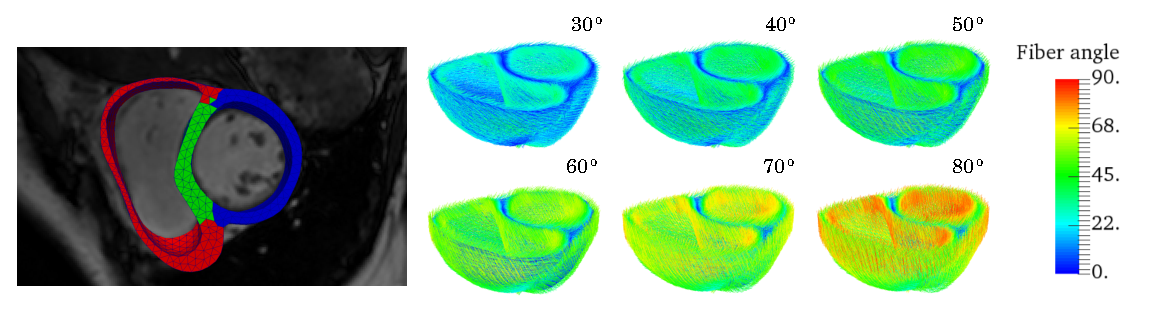
\includegraphics[width=\textwidth]{figures/fiber/fiber_v2}
\caption{\label{paper3:fig:fiber_angles} Left: finite
    element mesh of a biventricular geometry reconstructed from MR
    images separated into 3 material regions, namely, LVFW (blue),
    septum (green) and RVFW (right). Right: myocardial fiber
  orientation are assigned using the LDRB algorithm
  \citep{bayer2012novel} with an angle $+\alpha$ and 
  $-\alpha$ prescribed on the endocardium and epicardium, respectively. Here
  showing the fiber architecture for $\alpha$ ranging from
  $30^{\circ}$ to $80^{\circ}$ with increments of $10^{\circ}$, where
  the absolute value of the fiber angle is used as
  color-map.} 
\end{figure}





\subsection{Mechanical modeling}
\label{paper3:sec:mechanical_model}

We consider a configuration of a biventricular continuum body
$\mathfrak{B}$, which is a function $\kappa : \mathfrak{B} \rightarrow
\mathbb{R}^3$, and denote the reference and current configurations
by $\Omega_0 = \kappa_0 (\mathfrak{B}) $ and $\Omega = \kappa
(\mathfrak{B}) $, respectively. Letting $\Xvec$ and $\xvec$
be the coordinates of a given material point in the reference and
current configuration respectively, we have the corresponding
displacement field $\uvec = \xvec-\Xvec$, and the deformation gradient 
\begin{align}
  \F = \frac{\partial \uvec}{\partial \Xvec} + \I.
\end{align}
Mechanics of the heart wall was described using an active strain
formulation \citep{ambrosi2011electromechanical} that assumes a
multiplicative decomposition of the deformation gradient,
\begin{equation}
 \F = \F_e \F_a.
\label{paper3:eq:active_strain}
\end{equation}
Here, $\F_a$ is associated with an inelastic deformation resulting from the
actively contracting muscle fibers, whereas $\F_e = \F \F_a^{-1}$ is
associated with the elastic deformation that preserves compatibility
in the tissue, and passively carrying the mechanical load. We choose
$\F_a$ to have the specific form  
\begin{equation}
  \F_a = (1 - \gamma) \ef \otimes \ef  + \frac{1}{\sqrt{1 - \gamma}} (\I - \ef \otimes \ef),
 \label{paper3:eq:active_strain_Fa_gjerald}
\end{equation}
in which the parameter $\gamma$ is associated with the relative active
shortening along the muscle fibers. The same form of the active
deformation gradient has previously been applied in e.g
\citep{gjerald2014patient,balaban}.


We consider the transversely Holzapfel and Ogden hyperelastic material
\citep{holzapfel2009constitutive} model that has the strain energy
density function
\begin{align}
\label{paper3:eq:holzapfel_ogden}
\Psi(\F) = \frac{a}{2 b} \left( e^{ b (I_1  - 3)}  -1 \right)
 + \frac{a_f}{2 b_f} \left( e^{ b_f (I_{4\ef} - 1)_+^2} -1 \right),
\end{align}
where the invariants are given by
\begin{align}
  I_1 = \tr \C, \;\; I_{4\ef} = \ef \cdot (\C \ef).
\end{align}
Here $\C = \F^T\F$ is the right Cauchy Green tensor, and $\ef$ denotes
the unit fiber field in the reference configuration.
Within the active strain formulation, the strain energy depends only on
elastic deformations, and so the modified strain energy function
$\Psi = \tilde{\Psi}(\F_e)$ was used instead. 

For comparison, we also test the more frequently used active stress
formulation \citep{hunter1998modelling}. In this formulation, the total Cauchy
stress tensor is additively decomposed into a passive and an active component i.e.,
\begin{align}
  \Cauchy = \Cauchy_p + \Cauchy_a,
\end{align}
where the passive stress tensor is given by
\begin{align}
  \Cauchy_p = \frac{1}{J} \frac{\partial \Psi}{\partial \F}\F^T,
\end{align}
and the active stress tensor is given by
\begin{align}
  \Cauchy_a = T_a \left[\Fef \otimes \Fef +
   \eta\left(\I - \Fef \otimes \Fef \right)\right].
  \label{paper3:eq:active_stress}
\end{align}
Here $T_a$ is the magnitude of the active stress and $\eta$ controls
the amount of transverse active stresses.
Although active stresses, in principle, develop along the fiber
direction, studies have shown \citep{lin1998multiaxial} that active
stresses in the transverse direction are non-negligible due to
imperfect alignment of the muscle fibers. We therefore set $\eta =
0.2$ \citep{sundnes2014improved}, and note that transverse active
stresses are naturally embedded in the active strain formulation by
requiring $\mathrm{det}\;\F_a = 1$ .

Myocardium was assumed to be incompressible. The incompressibility was
enforced in the model using a two-field variational approach, in which
the term $-p(J-1)$ was added to the total strain energy with $p$
denoting a Lagrange multiplier that represents the hydrostatic
pressure. The deviatoric and volumetric mechanical responses were also
uncoupled by multiplicatively decomposing the deformation gradient
\citep{weiss1996finite}, 
\begin{align}
  \F = \F_{\mathrm{iso}}\F_{\mathrm{vol}}
  \label{paper3:eq:deviatoric_split}
\end{align}
and letting the strain-energy be a function of only isochoric
deformations i.e., $\Psi = \bar{\Psi}(\F_{\mathrm{iso}})$.
  
Ventricular base was fixed in the longitudinal direction and the
biventricular geometry was anchored by constraining the
epicardial surface using a Robin-type boundary condition with a linear
spring of stiffness $k=0.5$ kPa/cm$^2$ \citep{xi2016patient}.
Measured cavity pressure in the LV ($\plv$) and RV ($\prv$) were
applied as a Neumann condition at the endocardial surfaces.
The Euler-Lagrange equations in the Lagrangian form reads: Find
$(\uvec, p) \in V \times Q$ such that for all $ (\delta \uvec, \delta
p) \in V \times Q$ and $\left. \left( \uvec \cdot \N \right)
\right|_{\partial \Omega_0^{\mathrm{base}}} = 0$ ,

\begin{align}
  \delta\Pi(\uvec, p) &=
  \int_{\Omega_0} \left[ \FPiola: \nabla \delta \uvec  - \delta p (J - 1 ) - pJ\F^{-T}:\nabla \delta \uvec \right] \mathrm{d}V
  + \delta\Pi_{\text{ext}} = 0,
  \label{paper3:eq:force_balance}
\end{align}
with
\begin{align}
  \begin{split}
  \delta \Pi_{\text{ext}} &=
  \int_{\partial \Omega_0^{\mathrm{endo} \; \mathrm{LV}}} \plv J \F^{-T} \N \cdot \delta \uvec \mathrm{d}S \\ &+
  \int_{\partial \Omega_0^{\mathrm{endo} \; \mathrm{RV}}} \prv J \F^{-T} \N \cdot \delta \uvec \mathrm{d}S +
  \int_{\partial \Omega_0^{\mathrm{epi}}} k \uvec \cdot \delta \uvec \mathrm{d}S.
 \end{split}
  \label{paper3:eq:bndry_cond}
\end{align}

\noindent
Here $V = H^1(\Omega_0)$, completed with homogeneous Dirichlet boundary
data, $Q = L^2(\Omega_0)$, $ \N $ is the outward pointing unit normal
and  $\FPiola$ is the first Piola-Kirchhoff stress tensor.

\subsection{PDE-constrained optimization}
The ventricular mechanics model outlined in Section \ref{paper3:sec:mechanical_model}
contains model parameters that may vary from individual to
individual.
Calibration of these model (or control) parameters was achieved by solving a
PDE-constrained optimization problem, where we minimized a cost functional
representing the mismatch between the simulated and
observed data, subject to the constraint of satisfying
\eqref{paper3:eq:force_balance}-\eqref{paper3:eq:bndry_cond}.
The minimization problem can be formally stated as
\begin{equation}
  \begin{aligned}
    \label{paper3:eq:optimization_problem}
    & \underset{m}{\text{minimize}}
    & &  \mathcal{J}((\uvec, p), m) \\
    & \text{subject to}
    & & \delta \Pi(\uvec, p) = 0.
  \end{aligned}
\end{equation}
Here $\mathcal{J}$ is the objective functional that we want to
minimize, which depends on the state variable $(\uvec, p)$ and the
control parameter(s) $m$. The state variables may also depend on the
control parameters $(\uvec, p) = (\uvec(m), p(m))$. To ease
notation, this dependency is not explicitly stated here.

Minimization of the cost functional $\mathcal{J}$, should bring
the simulated results closer to the clinical observations. Therefore,
$\mathcal{J}$ should reflect a distance between the model and the data.  
Given a measurement point $i$, let $(\uvec^i,p^i)$ be the simulated state
variables at that point, and let $m^i$ represents any generic model
parameter, that we want to estimate. The cost functional is then
given by
\begin{equation}
  \mathcal{J}((\uvec^i,p^i), m^i)
  = \alpha \mathcal{J}_{\mathrm{volume}}((\uvec^i, p^i), m^i)
  + \beta \mathcal{J}_{\mathrm{strain}}((\uvec^i, p^i), m^i)
  + \lambda \mathcal{J}_{\mathrm{reg}}(m^i).
  \label{paper3:eq:total_functional}
\end{equation}
The first two terms represent the mismatch between simulated and
observed strains and volumes, whereas $\mathcal{J}_{\mathrm{reg}} $ is
a regularization term that penalizes non-smooth values of the control
parameter $m^i$ for numerical stability. The weights $\alpha, \beta$
and $\lambda$ control what terms is favored in the optimization.


The cavity volume was given by
\begin{equation}
  \tilde{V}_{\cdot} = - \frac{1}{3} \int_{\partial \Omega_0^{\mathrm{endo}\; \cdot}} (\Xvec + \uvec )J \F^{-T} \N \mathrm{d} S.
\end{equation}
This equation holds as long as the base remains flat and is located at the $x=
0$ plane. We let $\mathcal{J}_{\mathrm{volume}}$ be the sum of the
squared relative volume error in each chamber:
\begin{equation}
  \mathcal{J}_{\mathrm{volume}}((\uvec^i, p^i), m^i) =
  \left( \frac{V_{\text{LV}}^i - \tilde{V}_{\text{LV}}^i}{V_{\text{LV}}^i} \right)^2
  + \left( \frac{V_{\text{RV}}^i- \tilde{V}_{\text{RV}}^i}{V_{\text{RV}}^i} \right)^2.
  \label{paper3:eq:I_vol}
\end{equation}
Here, $(\tilde{V}_{\text{LV}}, \tilde{V}_{\text{RV}})$ and
$(V_{\text{LV}}, V_{\text{RV}}) $ are the simulated and measured
cavity volumes, respectively.

Volumetric averaged strains were computed in each material region
(i.e., LVFW, RVFW and septum) using end-diastole (ED) as
reference. Letting $\F_{\mathrm{ED}}$ be the deformation gradient
tensor associated with ED, the Green-Lagrange strain tensor with ED as
reference was given by $\tilde{\mathbf{E}} =
\frac{1}{2}(\F^T\F_{\mathrm{ED}}^{-T} \F\F_{\mathrm{ED}}^{-1} -\I)$.
Normal averaged strain along the circumferential direction
$\mathbf{e}_{\mathrm{circ}}$ in material region $\Omega_j$ was 
defined by 
\begin{align}
   \tilde{\varepsilon}_{j} = \frac{1}{|\Omega_j|}
   \int_{\Omega_j}\mathbf{e}_{\mathrm{circ}} \cdot \tilde{\mathbf{E}} \mathbf{e}_{\mathrm{circ}} \mathrm{d} V .
\end{align}
Correspondingly, the strain mismatch functional was given by the total
squared error between the simulated circumferential strain
$\tilde{\varepsilon}_{j}^i$ and the measured circumferential strain
$\varepsilon_{j}^i$ over all material regions 
\begin{equation}
  \mathcal{J}_{\mathrm{strain}}((\uvec^i, p^i), m^i)  =\sum_{j= 1}^{N} \left( \varepsilon_{j}^i -  \tilde{\varepsilon}_{j}^i \right)^2.
  \label{paper3:eq:I_strain}
\end{equation}
Finally, the regularization term was defined as the total squared distance
from the mean value, that is if $m^i = (m_1, \cdots, m_N)$, then
\begin{align}
\mathcal{J}_{\mathrm{reg}}(m^i) = \sum_{j=1}^{N} (m_j^i - \overline{m}^i )^2 , &&  \overline{m}^i = \frac{1}{N} \sum_{j=1}^{N} m_j^i.
\end{align}
As noted above, the purpose of this term is to avoid numerical
instabilities by penalizing large variations in the control parameters.




\subsection{Parameter estimation}
The pipeline for fitting the model to patient data was 
divided into two sequential phases; a passive phase where we estimated the
material parameters that define the passive behavior of the
myocardium, and an active phase where we estimated the amount
of active contraction.
In both cases, the control parameters were 
spatially resolved. During the passive phase the control parameter was
allowed to vary spatially on the LV (LVFW+septum) and RV segments, while in the active
phase the LV was separated into LV free wall and septal segments, which provided
additional degree of freedom to allow for non-homogeneous LV contraction.


Geometries used in the simulation were reconstructed from medical
images. These geometries are, in principle, not load-free. Hence, we
need to estimate the unloaded (zero pressure) geometries, which  will
revert  back to the original reconstructed geometries when loaded with
the measured pressure. Several methods exists for estimating the
unloaded geometry \citep{govindjee1996computational,gee2010computational}. 
Among the most simplest ones is the backward displacement method
\citep{sellier2011JFS,bols2013computational} that can also be used to
incorporate residual stresses into the finite element models by
simulating tissue growth \citep{Genet2015JB}. Nevertheless, this
inverse problem (of finding the unloaded geometry) has  been shown to
produce non-unique solutions, especially when buckling is present
\citep{govindjee1996computational}, although relaxation techniques can
be used to improve convergence and stability \citep{Rausch2017JB}. For
the case of a bi-ventricular geometry, buckling may occur due to the
thin RVFW and a high RV pressure. For this reason, we choose a simpler
approach to estimate  the unloaded configuration. As shown in the left
of Figure \ref{paper3:fig:pipeline}, we start by applying one iteration of
the backward displacement method with initial values prescribed for
the material parameters followed by the material parameter estimation
as outlined below. This will result in a deflated geometry as shown in
the right of Figure \ref{paper3:fig:pipeline}. A sensitivity analysis
(\ref{paper3:sec:unloaded_sens}) was conducted to assess how the choice of
the initial material parameter values affects our results. 


Four material parameters i.e., $a$, $a_f$, $b$ and $b_f$
\eqref{paper3:eq:holzapfel_ogden} have to be estimated in the passive phase.
Due to the sparsity of passive data used for the optimization, if we
let all these parameters vary freely, we may end up in a situation
where multiple parameter sets will equally minimize the cost functional, and the
optimal control will depend heavily on the initial guess of the optimization.
We therefore restricted our control parameter to be only the linear
isotropic parameter with an initial guess $a=1.291$kPa, and have the
remaining parameters fixed according to \citep[Table 2, case
P2]{asner2015estimation}. The weights were set $\alpha = 1.0, \beta =
0.0$ and $\lambda = 10^{-6}$ in \eqref{paper3:eq:total_functional} so that
only ED volumes were used for fitting.  
Since fitting the left and right ventricular
end diastolic volumes might require different material
properties of the left and right ventricular wall, the parameter $a$ was
spatially resolved with one parameter associated with the LV (LVFW +
septum) and one parameter associated with the RVFW


In the active phase, the optimized material parameters were fixed and
the relative active fiber shortening $\gamma$ in
\eqref{paper3:eq:active_strain_Fa_gjerald} was chosen as control
parameter. For this phase, the weights in \eqref{paper3:eq:total_functional}
were set to $\alpha = 0.1,  \beta = 1.0$ and $\lambda = 10^{-4}$, so
that both strain and volume are considered in the optimization. This
choice of weighting was made ad hoc, reflecting the relative size of
the different terms in the cost functional. It should also be noted
that the volume functional in \eqref{paper3:eq:I_vol} is a relative error
while the strain functional in \eqref{paper3:eq:I_strain} represents a total
error. 

For each time point, we estimated $\gamma$ locally in the LVFW, RVFW
and septum. The initial guesses for the optimization were set to zero
in the first iteration. In subsequent iterations, the initial guesses
were set to the optimized values found in the previous iteration.
Note that in the case when active stress formulation was used instead,
the parameter $T_a$ in \eqref{paper3:eq:active_stress} was used as the
control parameter and estimated in a similar fashion. 

A schematic illustration of the full optimization pipeline is provided
to the left in Figure \ref{paper3:fig:pipeline}.

\begin{figure}[htbp]
  \centering
  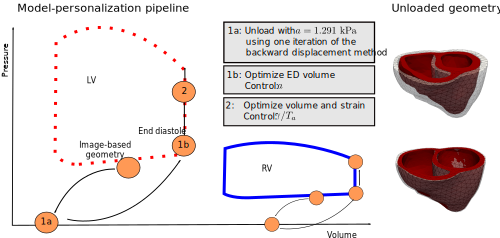
\includegraphics[width=\textwidth]{figures/models}
  \caption{\label{paper3:fig:pipeline}To the left we see the
    model-personalization pipeline. The image-based
    geometry corresponds to some image frame taken at mid diastole. An
    estimate of the unloaded geometry was found by applying one
    iteration of the backward displacement method using $a = 1.291$ kPa
    according to \citep{asner2015estimation}, followed by an estimation
    of $a$ by minimizing the fit of the end-diastolic volumes. During
    systole, both cavity volumes and circumferential strain were used in
    the optimization to determine the amount of active contraction in
    terms of the active control, which are respectively  $\gamma$ and $
    T_a$ in the active strain and active stress formulation. To the
    right we show a comparison of the unloaded geometry for CASE3. The
    upper figure shows the resulting unloaded, zero pressure geometry in
    red and the the original image-based geometry in transparent, while
    the bottom figure shows the unloaded geometry, inflated to the target
    pressure in the image-based geometry, and the original image-based
    geometry in transparent for comparison.}
\end{figure}

\subsection{Mechanical Analysis}

%\subsubsection{Stress analysis}
% Abnormalities in ventricular wall stress is believed to be responsible
% remodeling processes associated with heart failure. It is therefore of
% interest to compute the stresses in the personalized simulations.
For an incompressible, hyperelastic, continuum body, the total Cauchy
stress tensor is given by
\begin{align}
  \Cauchy = \frac{1}{J} \frac{\partial \Psi(\F)}{\partial \F} \F^T - p\I.
  \label{paper3:eq:total_cauchy_stress}
\end{align}
With the decoupling of the isochoric and volumetric deformation
according to \eqref{paper3:eq:deviatoric_split},
the first term in \eqref{paper3:eq:total_cauchy_stress} represents the
deviatoric stresses and $p$ is the hydrostatic pressure. Myofiber
stress was computed by first a push forward of the fiber field to the current
configuration, $\mathbf{f} = \F \mathbf{f}_0$, and then an inner
product with the stress tensor $\Cauchy_{\mathbf{f}} = \mathbf{f}
\cdot \Cauchy \mathbf{f}$. The average fiber stress in a given region
$\Omega_j$ was computed by integrating the fiber stress over that
region and dividing by the volume i.e.,
$\overline{\Cauchy_{\mathbf{f}}}^{\Omega_j} = | \Omega_j |^{-1}
\int_{\Omega_j} \Cauchy_{\mathbf{f}} \mathrm{d} V$.

%\subsubsection{Contraction analysis}
The control parameter in the active phase represents an index of
contractility \citep{finsberg2017estimating}, meaning that the higher
the value of the control parameter, the more forcefully the myocardium is
trying to contract against the external loads. To separate between the LV and
RV contractility, we extracted the average value of this control parameter in these
two segments. Another index of contractility is the end systolic
elastance \citep{sagawa1977end}, which we have also estimated in the LV and
RV by perturbing the loading conditions at the end systolic state and
estimate the slope of the resulting pressure-volume
relationship \citep{finsberg2017estimating}.


\subsection{Implementation details}
The force-balance equations were solved using the finite element
method, whereby the displacement and hydrostatic pressure fields were
interpolated using piecewise quadratic and linear basis functions,
respectively. These mixed elements, known as the Taylor-Hood finite
elements \citep{hood1974navier}, are known to satisfy the discrete
inf-sup condition \citep{chapelle1993inf} and leads to a stable
discretization. The solver was implemented in FEniCS
\citep{logg2012automated}, which is an open-source platform for
solving PDEs using the finite element method. Nonlinear systems of
equations were solved using Newton's method,
and a distributed memory parallel LU solver\citep{li2003superlu_dist}
was used to solve the linear systems.


To solve the optimization problem \eqref{paper3:eq:optimization_problem} we
applied a sequential quadratic programming algorithm (SQP)
\citep{kraft1988software}. This gradient-based optimization
algorithm requires the functional gradient, that is the derivative
of the functional $\mathcal{J}$ in \eqref{paper3:eq:total_functional}, with
respect to the control parameters. This gradient was
computed by solving an automatically derived adjoint equation using
dolfin-adjoint \citep{farrell2013automated}.
The full source code is publicly
  available\footnote{\url{https://bitbucket.org/finsberg/pulse_adjoint}}. 

\section{Results}
\label{paper3:sec:results}
In this section we present the results from the model personalization
process. Results of the data matching are 
presented in Section \ref{paper3:sec:data_asssim}, together with a validation of the
model and analysis of the solver performance. To validate the model we compare the
simulated and measured longitudinal strain which was not used in the
optimization. In Section \ref{paper3:sec:mech_analysis} we present the results of the
extracted mechanical features such as indices of contractility and
fiber stress.  We also investigated the efficiency of the algorithm and the effect of mesh refinement, and
found that the chosen refinement level was sufficient to yield
convergent solutions.

\subsection{Data assimilation, validation and solver performance}
\label{paper3:sec:data_asssim}
\label{paper3:sec:validation}
\label{paper3:sec:sys_perform}
%The simulated pressure-volume (PV) loops of LV and RV were in close
%agreement with the measured PV loops, as shown in the left panel of Figure
%\ref{paper3:fig:data_matching}. 
The simulated and measured pressure-volume (PV) loops of the RV and LV, as well as circumferential strain in the LV, septum
and RV are shown in Figure \ref{paper3:fig:data_matching}. We found that the fit of the data was highly dependent
on the choice of fiber angles, which affects both volume change and circumferential shortening. Plotting the average value of the
volume cost functional (as defined in \eqref{paper3:eq:I_vol}) for each
choice of fiber angles as shown in the upper right panel in
Figure~\ref{paper3:fig:data_matching}, revealed that the optimal value of
$\alpha$ lies in the range $70^{\circ}-80^{\circ}$ for all 3 cases.


\begin{figure}[htbp]
 \centering
  \includegraphics[width=\textwidth]{figures/data_matching}
  \caption{\label{paper3:fig:data_matching}Results of the gradient-based
    minimization of model-data mismatch for different choice of fiber
    angles. Left: simulated (color lines) and measured (black circles)
    PV loops in the LV (top row) and RV (bottom row). Center:
    simulated (color lines) and measured (black circles)
    circumferential strain in the LV (top row), RV (middle row ) and
    septum (bottom row). Right: average values of cost functional for
    the volume (top row) and strain (bottom row), for each choice of
    fiber angle.}  
\end{figure}


Although available, we chose not to use longitudinal strain data in the
optimization. Therefore, the comparison of model-predicted
longitudinal strain with the measurements serves as a validation of the
model-personalization process. The simulated and measured LV
longitudinal strain curves are shown in Figure
\ref{paper3:fig:fiber_long}. We note that the fit in all regions was again highly sensitive
to the choice of fiber angle. Choosing $\alpha = 70^{\circ}$ produced the best
fit for the LV longitudinal strain for CASE1 and CASE3, while an angle
$60^{\circ}$ gave the best fit for CASE2. The Septal and RV
longitudinal strain was best fitted with $\alpha = 80^{\circ}$.  


\begin{figure}[htbp]
 \centering
  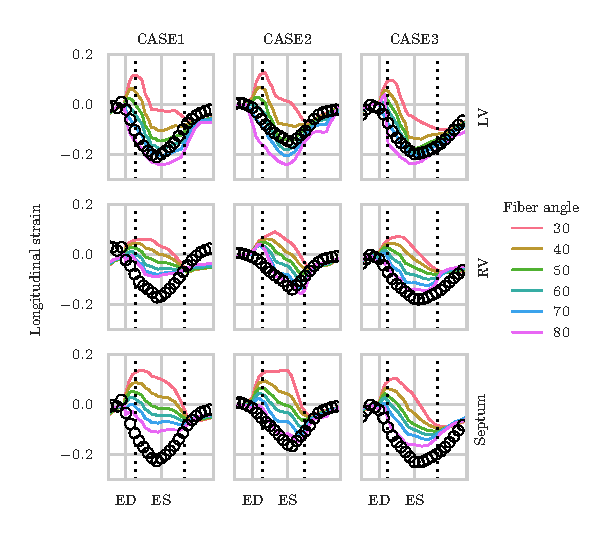
\includegraphics[width=\textwidth]{figures/longitudinal_strain}
  \caption{\label{paper3:fig:fiber_long}Validation of the
    model-personalization process using simulated and measured
  longitudinal strain which was not used in the optimization. Upper,
  middle and lower panel show the longitudinal strain
  curves for different choice of fiber angles in the LV, RV and septum respectively.}
\end{figure}

% \subsection{Solver performance}
We further evaluated the solver performance in the optimization process.  In this work, all computations were performed on a computing cluster using one node
with 8 cores. In Table \ref{paper3:tab:timings} we present timings for evaluation of
the forward model (i.e., evaluation of the cost functional), timings for
evaluation of the gradient, as well as the average number of such
evaluations and the standard deviations. These timings are shown for
optimizations using the original and refined meshes with a fiber
angle of $60^{\circ}$. 


\begin{sidewaystable}
\caption{Timings for evaluation (eval) of the forward model and the gradient,
  running on one computing node with 8 cores for the different subjects
  with different mesh resolutions. The average number of forward
 and gradient evaluations for each measurement points are also shown
 along with the standard deviations.}
\begin{tabular}{lllllll}
\toprule
  Patient ID   & $\#$ elements   & forward eval time (s)
  & $\#$ forward eval   & gradient eval time (s)
  & $\#$ gradient eval & Total run time (h)  \\
  \midrule
  \multirow{2}{*}{CASE1}
               &7362  & 32 $\pm$ 19.8   & 9 $\pm$ 1.6  & 9 $\pm$ 0.1  & 8 $\pm$ 1.5 & 1.97\\
               &58896 & 668 $\pm$ 529.8 & 9 $\pm$ 1.7  & 81 $\pm$ 1.3 & 7 $\pm$ 1.6 & 36.1\\
  \hline
  \multirow{2}{*}{CASE2}
               & 4755  & 19 $\pm$ 9.6    & 9 $\pm$ 2.1  & 8 $\pm$ 0.1  & 8 $\pm$ 2.0 & 1.88\\
               & 38040 & 387 $\pm$ 325.8 & 9 $\pm$ 2.5  & 47 $\pm$ 0.4 & 8 $\pm$ 2.2 & 32.6\\
  \hline
  \multirow{2}{*}{CASE3}
               & 4377  & 17 $\pm$ 5.3    & 10 $\pm$ 2.1 & 8 $\pm$ 0.9  & 8 $\pm$ 2.1 & 1.35\\
               & 35016 & 259 $\pm$ 146.3 & 9 $\pm$ 2.4  & 42 $\pm$ 0.7 & 8 $\pm$ 2.2 & 15.6\\
\bottomrule
\end{tabular}
\label{paper3:tab:timings}
\end{sidewaystable}



\subsection{Mechanical analysis}
\label{paper3:sec:mech_analysis}
\subsubsection{Cardiac contraction}
The estimated active strain parameter $\gamma$ in
\eqref{paper3:eq:active_strain_Fa_gjerald}, which served as the control parameter
during the optimization in the  active phase, is plotted for various fiber angles to the
left in Figure \ref{paper3:fig:mechanical_analysis}. This parameter
varies regionally in the LVFW, septum and RVFW, but is shown here as
an average in the LV containing LVFW + septum (top) and RV containing
only RVFW (bottom). As shown in the figure, time-variation and
magnitude of $\gamma$ were similar in the 3 cases and insensitive to
the prescribed fiber angles. 

\begin{figure}[htbp]
  \centering
  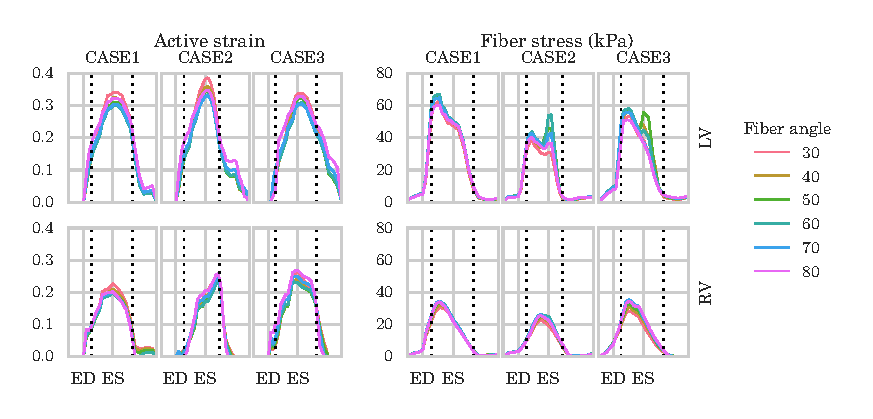
\includegraphics[width=\textwidth]{figures/mechanical_analysis}
  \caption{\label{paper3:fig:mechanical_analysis}To the left, average traces of the active strain
    parameter $\gamma$ in \eqref{paper3:eq:active_strain_Fa_gjerald} in the
    LV (top) and RV (bottom) for different choice of fiber angle. To
    the right average traces of Cauchy fiber stress in the  LV (top)
    and RV (bottom) for different choice of fiber angle. The
    fiber angles were defined symmetrically across the wall with a
    negative angle on the epicardium and a positive angle on the
    endocardium ranging from $30^{\circ} - 80^{\circ}$ with increments
  of $10^{\circ}$. On the $x-$axis we plot the normalized time with
  respect to end-diastole (ED) and end-systole (ES). Horizontal dotted
lines indicate timings of opening of the aortic and mitral valve.}
\end{figure}

Time traces of the active strain parameter $\gamma$ found in the LV
and RV are plotted together for the $60^\circ$ fiber angle case in the
left of Figure \ref{paper3:fig:active_stress_conv} in order better compare
their differences. A similar plot of the active stress parameter $T_a$
in logarithmic scale is also shown in the same figure. As shown in
the figure, the time-variations of $T_a$ and $\gamma$, which are
indices of cardiac contractility, were largely similar between the LV
and RV with peak values located approximately at end-systole. Peak
values found in the RV were, however, lower than those found in the
LV. These findings were consistent across all the 3 cases.

\begin{figure}[htbp]
  \centering
  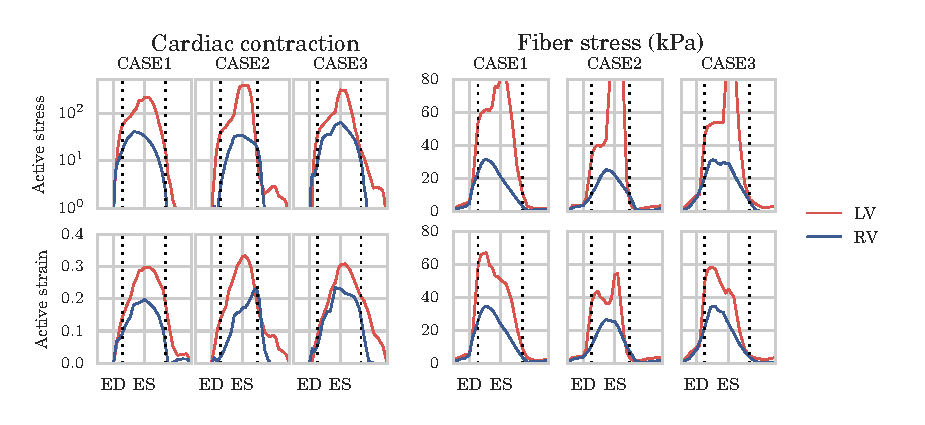
\includegraphics{figures/mechanics_mesh_conv}
  \caption{\label{paper3:fig:active_stress_conv}Comparison of fiber stress
    and cardiac contraction using the active strain and active stress
    approach using $60^{\circ}$ fiber angle.
    To the left, average traces of the active stress (top) parameter $T_a$
    in \eqref{paper3:eq:active_stress}, and the active strain (bottom)
    parameter in \ref{paper3:eq:active_strain_Fa_gjerald}.  The active
    stress parameter, with unit kPa, is plotted on a logarithmic scale
    for easier comparison with the active strain parameter.
    To the right, estimated
    Cauchy fiber stress using the active
    stress (top) and active strain formulation (bottom).  On the $x-$axis we
    plot the normalized time with respect to end-diastole (ED) and
    end-systole (ES). Horizontal dotted lines indicate timings of
    opening and closing of the aortic valve.}
\end{figure}


\subsubsection{Fiber stress}
Time traces of the average Cauchy fiber stress are shown on the right
of Figure \ref{paper3:fig:mechanical_analysis} for different fiber angle
variations.  Only very small variations in the average fiber stress
were found with respect to the choice of fiber angle in the
optimization process. Snap shots of the fiber stress distribution at
ED and ES are plotted in Figure \ref{paper3:fig:mesh_res_stress_snapshots}
for the  $60^{\circ}$ fiber angle case. Regional variation of fiber
stress was largely consistent between the 3 cases with pockets of high
and low stresses found, respectively, at the apex-epicardial and
endocardial regions at ES.

In Figure \ref{paper3:fig:active_stress_conv}, we compare the average fiber stress
time variation found using the two different active contraction
formulations, either active strain or active stress. As shown in the figure, fiber stress computed using
active stress and active strain formulations behaved similarly with
time. Similar regional variation was also found where both
formulations predicted higher fiber stress in the LV than 
the RV. Peak fiber stress predicted in the LV, however, was different in
the two formulations with higher stress occurring at isovolumic
relaxation in the active stress formulation. 

\begin{figure}[htbp]
  \centering
  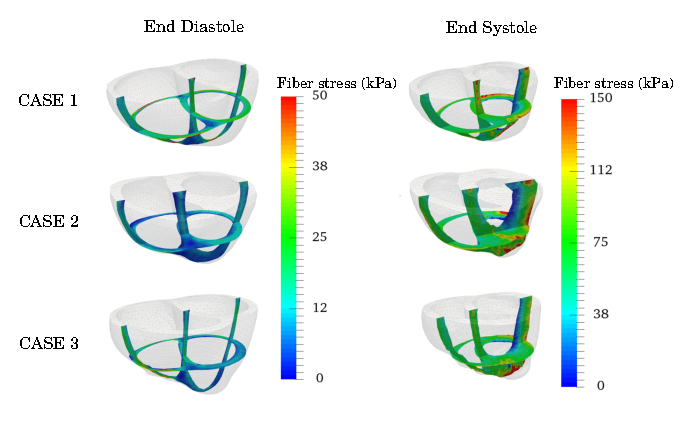
\includegraphics{figures/snapshots/stress}
  \caption{\label{paper3:fig:mesh_res_stress_snapshots}Snap shots of the end
    diastolic and end systolic configuration and the estimated fiber
    stresses shown as color-map.}
\end{figure}


The specific average value of the end-diastolic and end systolic fiber
stress for the case of a $60^{\circ}$ fiber angle are displayed in
Table \ref{paper3:tab:fiber_stress}, showing small variability between patients, despite differences in
individual PV loops.  

\begin{table}
  \centering
\caption{Average LV and RV fiber stress and end diastole and end systole}
\begin{tabular}{lrrrr}
\toprule
  Patient ID   &   LV (ED) &   RV (ED) &   LV (ES) &   RV (ES) \\
  \midrule
  CASE1        &      5.76 &      4.87 &      48.3 &      19.2 \\
  CASE2        &      4.04 &      3.57 &      54.4 &      22.7 \\
  CASE3        &      9.94 &      8.34 &      40.3 &      18.2 \\
  \hline
  Average $\pm$ std & 6.58 $\pm$ 2.48 & 5.59 $\pm$ 2.01 & 47.65 $\pm$ 5.74 & 20.03 $\pm$ 1.91 \\
\bottomrule
\end{tabular}
\label{paper3:tab:fiber_stress}
\end{table}


\subsubsection{Ventricular Elastance}

Table \ref{paper3:tab:elastance} shows the estimates of ES elastance in the
LV and RV that were computed using the active strain formulation. 
The table shows the average $\pm$ one standard deviation of the ES
elastance over various fiber angles. Elastance was consistently
found to be $\sim 10$ times larger in the LV than in the RV, and was 
largely insensitive to the prescribed fiber angle as indicated by the
small standard deviation.  

\begin{table}
  \centering
\caption{LV and RV end-systolic elastances estimated
  by perturbation of model at the end-systolic state. Average values and
  standard deviation with respect to varying fiber angle are shown.}
\begin{tabular}{lll}
\toprule
 Patient ID   & LV (kPa/ml)     & RV (kPa/ml)     \\
\midrule
 CASE1        & 1.96 $\pm$ 0.06 & 0.23 $\pm$ 0.02 \\
 CASE2        & 1.94 $\pm$ 0.14 & 0.18 $\pm$ 0.01 \\
 CASE3        & 1.52 $\pm$ 0.07 & 0.21 $\pm$ 0.01 \\
\bottomrule
\end{tabular}
\label{paper3:tab:elastance}
\end{table}


\section{Discussion}
\label{paper3:sec:disc}
In this study, we have presented a novel and highly efficient method for non invasive
personalization of an image-based bi-ventricular mechanics model based
on regional measurements of circumferential strain, as well as global
measurements of volumes and pressures in the LV and RV.
A gradient based optimization method was used to
minimize the model-data mismatch by solving a PDE-constrained optimization problem for
each measurement point in order to calibrate model
parameters. Passive material parameters and an unloaded
(zero-pressure) geometry were estimated using the bi-ventricular
geometry that was reconstructed from MR images acquired at late
diastole. Time variation of an active contraction parameter was
estimated throughout the cardiac cycle starting from ED. 

This framework was applied using measurements from three normal subjects to
extract estimates of regional fiber stress as well as indices of myocardial
contractility.  Sensitivity analysis of the model outputs with respect
to the choice of fiber angle distribution, mesh resolution and active
formulation were also conducted. The described framework is
effective and efficient in capturing cardiac mechanical behavior
throughout the cardiac cycle, and gave low patient-to-patient variabililty in the extracted mechanical features.  As such, it has potential clinical utility in
the quantification of contractile function and myocardial stress
{\it in vivo} and the potential differentiation of pathological states.



\subsection{Data compatibility and multi-objective optimization}

The objective functional in  problem \eqref{paper3:eq:optimization_problem}
consists of a weighted sum of different objective functionals.
Such problems are referred to as multi-objective optimization problems
\citep{marler2004survey}.  While it is possible to perfectly match the
strain or volume data individually with the chosen control parameters (data not shown), there is
expected to be a trade-off when fitting both the volume and strain data
 in a combined objective functional. In such
cases, a single, unique optimum does not always exist, but rather
a family of so called Pareto optimal solutions can be found \citep{marler2004survey}.
The particular solution found will depend on the chosen weights of
each objective.

In a previous study \citep{balaban}, the weights in the total
functional given in \eqref{paper3:eq:total_functional} were determined by performing an
exhaustive search, testing several combinations of weights of the strain and volume
functionals, and choosing the corner-point of strain versus volume
error curve. However, the weights will depend on the data 
source, and in our case choosing the weights proposed in \citep{balaban},
resulted in an excellent fit of the volume, while a relatively
poor fit of the strain, and hence a higher weight was chosen for the
strain. Nevertheless, neither was captured exactly, and which data
source is more important for model utility remains to be
determined. In addition, other general methods for solving
multi-objective optimization problems \citep{marler2004survey} may be
superior to the weighted sum method used here, and will be considered
in future studies. 

\subsection{Fiber angle sensitivity}
In this work, we applied a rule-based algorithm \citep{bayer2012novel} to
assign myocardial fiber orientations to the bi-ventricular geometries,
and investigated the sensitivity of the data matching and the extracted
mechanical features to the choice of fiber field.
Different fiber fields, in which the fiber angle varies linearly
across the myocardium wall from $\alpha$ at the endocardium to
$-\alpha$ at the epicardium were tested, for the range $30^\circ \leq \alpha \leq
80^\circ$. Our results show that $\alpha$ has to be in the upper part
of the range i.e., $70-80^{\circ}$, in order to fit the PV loop and
circumferential strain measurements simultaneously.
The validation study (Section \ref{paper3:sec:validation}), where we compared
our model results with the longitudinal strain, confirms this finding. 

This highlights a major challenge in building accurate mechanics
models of the myocardium.  The choice of fiber field is very
important, as it controls the amount of longitudinal and radial
shortening during contraction. Unless the correct fiber
field is used, strain measurements cannot be reproduced simultaneously
in the model with the measured pressure volume relationships.
Accurate measurements of the underlying ventricular microstructure are
lacking, however, and therefore, rule-based methods
\citep{bayer2012novel} are often the only alternative to prescribe
muscle fiber field in subject-specific modeling of cardiac mechanics. 
Our fundamental knowledge of the myocardial
architecture is based largely on early histological studies
\citep{streeter1969fiber}, which found that the muscle fiber
orientation varies linearly across the myocardial wall  with an angle
$\alpha = 60^{\circ}$ at the endocardium $\alpha = -60^\circ$ at the
epicardium. This fiber field is often prescribed in ventricular models
without questioning. On the other hand, diffusion tensor MRI (DT-MRI) is now
becoming an important tool to measure fiber orientations and could
potentially do so \textit{in vivo} \citep{toussaint2013vivo}.

More recent histological
studies \citep{legrice1995laminar} on the canine left ventricle have shown that the muscle
fibers are more longitudinally oriented at the subendocardium and
subepicardium than those obtained using DT-MRI, and such fiber orientation can better
reproduce the longitudinal motions observed in the
experiments\citep{wang2015image}. Our results support this finding. 

A few hypotheses on the basis of cardiac muscle fiber orientation in
the ventricles have been put forward. 
For example, it has been hypothesized that myocardial fiber orientations adapts to
achieve a minimal fiber-cross fiber shear strain during the cardiac
cycle \citep{kroon2009computational}.
While our results showed that the active strain parameter $\gamma$
varied a little with respect to the different fiber angle $\alpha$
prescribed in the model, they also show that the peak active strain
$\gamma$ is lowest when $\alpha$ lies between $60^\circ$ and
$70^\circ$ in all 3 cases. This finding suggests that the tight range
of $\alpha$ found here is optimal in the sense that the active
shortening necessary to produce the same stroke volume is at its
minimum. 


\subsection{Fiber stress}


As there is no direct way to measure myocardial fiber stresses, we
have compared our results with other patient specific modeling
studies. The range of reported values for humans are
broad, and are mostly confined to the LV. For example,
\citep{genet2014distribution} reported fiber stress computed at ED
($2.21 \pm 0.58$kPa) and ES ($16.64 \pm 4.73 $kPa) in normal humans,
whereas \citep{scardulla2016evaluation} conducted a stress analysis on
healthy bi-ventricles and found that wall stress at ES was $65.7 \pm
12.3$ kPa in the LV and $23.6 \pm 14.2$ in the RV. 

Our estimated average fiber stresses (Table \ref{paper3:tab:fiber_stress})
are well within the range of values reported in these studies. Fiber
stress distributions at ED and ES (Figure
\ref{paper3:fig:mesh_res_stress_snapshots}) are also consistent in the three
subjects investigated here. Furthermore, our results also show small
variations in fiber stress with respect to the choice of fiber
field. Fiber stresses obtained from active strain and stress
formulations are also comparable during late diastole and early
systole. A large difference in the fiber stress between these two
formulations, however, can be found at late systole and during the
isovolumic relaxation when the ventricles are in their most compressed
state. In particular, the active stress formulation produces elevated
stresses during this time interval. The same phenomenon was observed
in a sensitivity analysis (\ref{paper3:sec:unloaded_sens}) on the initial
passive material parameter $a$ used to find the unloaded geometry. We
found that the elevated stresses are always accompanied by very
high hydrostatic pressure $p$, suggesting that the enforcement of
incompressibility, which does not hold {\it in vivo} due to blood
perfusion in the myocardial wall, is causing this artifact.  Future studies are 
needed to examine the effect of compressibility to our results.  

\subsection{Contractility}
Higher value of the active strain parameter $\gamma$ or the active
stress parameter $T_a$ indicates that the myocardium is contracting
more forcefully and our results also suggest that the
LV generates a higher contractile force per myocardial volume than the RV. 
One of the underlying mechanisms that modulate the contractile forces
is calcium dynamics \citep{hunter1998modelling,
  ambrosi2011electromechanical}, and while $T_a$ and $\gamma$ cannot be
directly compared to the calcium concentration because of the
difference in units, their time traces have similar shapes when
compared to the calcium transient. 
This finding is independent of  the prescribed fiber field and the initially assigned passive material
parameter $a$, as shown in \ref{paper3:sec:unloaded_sens}.  Further investigation of these estimates is needed, but we hypothesize that these measurements may provide useful biomarkers.  Due to the observed  consistent results in normal patients, even for wide ranging PV loops,  these estimates of contractility could therefore potentially serve as important diagnostic
estimates in cases where disease alters myocardial contractility.
 
 %[{\bf Not entirely clear of this statement - is it because the contractility  found in
%wide ranging PV loops in different cases are consistent with the elastance,  then we can use it as a %biomarker?}]}


\subsection{Elastance}
End systolic elastance is widely recognized as an important determinant of
systolic function \citep{sagawa1977end}. However, it's use in clinical
practice is limited due to the need for invasive measurements of pressure
and volume in response to varying loading conditions.

Here we have simulated a change in loading condition by perturbing
only the ES pressure (and fixing other quantities) and computing the ES
elastance from the slope of the resulting pressure-volume
relationship. This approach has been previously applied to obtain LV
ES elastance \citep{finsberg2017estimating}, but has not been applied
to find RV ES elastance in bi-ventricular geometries. 

The LV ES elastance estimated here, ranges from
approximately $1.0$ to $2.0$ kPa/ml, which is higher than values previously measured
in normal human hearts which ranges from $0.26$ to $0.4$ kPa/ml \citep{chen1998coupled}.

There are few reported values of normal human RV elastance.
However, \citep{brown1988human} reported values of the maximal RV
elastance in the range of 0.32 -1.23 mmHg/ml/ml$^2$ in normal
humans. Using a body surface area of 2 m$^2$ (typical in humans), this
range translates to 0.08 - 0.32  kPa/ml. Our estimated values $\sim
0.2$ kPa/ml  is well within this range. It should be noted here that
our estimates of ES elastance do not take into account of any
physiological aspect of the myocytes, such as changes in active
tension in response to changes in loading condition. 

\subsection{Limitations and future directions}

In this work, we clearly see a variability of model-data fit with
respect to choice of the fiber angle,
suggesting that the fiber field can be calibrated to better fit the
data. Here, we have only prescribed a linear transmural fiber angle
variation that has opposite signs at the endo- and epicardium in both
LV and RV. Dissection studies, however, generally found that the
fibers are more circumferentially oriented at the subepicardium and
more longitudinally orientated at the subendocardium in the RV
\citep{ho2006anatomy}. This suggests that one should also consider
non-symmetric fiber fields across the wall as well as different fiber
field in the LV and RV. We seek to investigate these issues in future
studies, possibly together with in vivo measures of fiber angles. 

While we were able to obtain stress measures across a small cohort of healthy subjects that were
both internally consistent as well as in broad agreement with other
published studies, the effect of our modelling assumptions remains to
be determined.  Here we used an incompressible model of the
myocardium, even though it is well known that the myocardium is 
compressible due perfusion of blood. Future studies should investigate
the role of compressibility, and in particular how fiber stress is
altered when the material is allowed to compress. We clearly see stress effects
related to the hydrostatic term in our model, and this will be
investigated more closely in future studies.

The late diastolic pressure-volume curve is fitted by estimating one
material parameter, while fixing the remaining parameters to previously
reported values \citep{asner2015estimation}. This is a limitation in our
study, and future studies will be geared towards reducing the need for fixing
these model parameters by incorporating more clinical data or by
revising the constitutive model.  In particular, the incorporation of
diastolic strains may be useful in more clearly defining material properties.

The simple estimation of unloaded configuration using only
one iteration of the backward displacement method can be used with
different initial material parameters and still recapitulate the
end-diastolic volumes with different optimized material parameters.
Several studies have jointly estimated
the unloaded left-ventricular geometry and material parameters
\citep{nikou2016effects, finsberg2017estimating, asner2015estimation},
but estimation of the unloaded configuration with
bi-ventricular geometries is not a well-posed problem, since buckling of
the RV free wall might occur. More work on formulating well-posed
algorithms for determining the unloaded configuration should be
considered in future studies.

Finally, in this study we only considered three normal
subjects, and in the future we would like to apply this framework to more
individuals and use it to study larger cohorts as well as patients with
cardiac pathology.


\section{Conclusion}
\label{paper3:sec:concl} 
Patient-specific simulations can now be assembled via adjoint-based
data assimilation techniques, using no more than a few hours on a
regular laptop. From these simulations we are able to extract
information about myocardial contractility and fiber stress which
shows low variability in the modeling choices that we make. Validation of
these models should be the main objective in the years to come in
order to translate cardiac computational modeling into clinical utility.


\section*{Acknowledgments}
This study was funded by Research Council of Norway: Center
for Biomedical Computing at Simula Research Laboratory and Center
for Cardiological Innovation at Oslo University Hospital.
Computations were performed on the Abel supercomputing cluster at
the University of Oslo via Notur project nn9249k. This study was also
partially supported by Singapore Ministry of Health's National
Medical Research Council (NMRC/OFIRG/0018/2016, Zhong), Goh
Cardiovascular Research Award (Duke-NUS-GCR/2013/0009, Zhong),
AHA SDG 17SDG33370110 (Lee) and R01-HL-134841 (Lee).



\section{Appendix}


\subsection{Sensitivity to unloaded configuration}
\label{paper3:sec:unloaded_sens}

The choice of initial material parameter $a$ in the unloading algorithm
will influence the estimated unloaded configuration. A softer material
will result in a lower unloaded volume, hence the optimized material
parameter will be softer to compensate for the greater volume increase
from the reference to the end diastolic state. In the results
presented in this study the value $a=1.291$ kPa was chosen based on
a parameter set used in \citep{asner2015estimation}.

To analyze the sensitivity of the results to the choice of material
parameters used to unload the geometry, we unloaded the geometries
using four different material parameters, i.e $a = 0.5, 1.0, 2.0$ and
$4.0$ kPa, and evaluated the corresponding model outputs. The resulting
optimized material parameters, unloaded cavity volumes and value of the
mismatch functional during the passive phase are shown in Table
\ref{paper3:tab:optmal_material_params_start}.


\begin{table}
  \centering
\caption{Optimized material parameters in kPa for different choice of
  unloaded configuration.}
\begin{tabular}{lrrrrrr}
\hline
  Patient ID   &   Initial $a$ &   $a_{\mathrm{LV}}$ &   $a_{\mathrm{RV}}$
  &   $\mathcal{J}_{\mathrm{data}}$ (passive) &   $V_0^{\mathrm{LV}}$ &   $V_0^{\mathrm{RV}}$ \\

\hline
 CASE1 & 0.5 & 0.05   & 0.321 & 0.000551 & 36.2 & 53.8 \\
 CASE1 & 1   & 0.165  & 0.699 & 7.13e-08 & 40.4 & 56.6 \\
 CASE1 & 2   & 0.64   & 1.49  & 1.81e-07 & 45.9 & 60.5 \\
 CASE1 & 4   & 1.92   & 2.91  & 2.46e-07 & 52.8 & 65.4 \\
 CASE2 & 0.5 & 0.05   & 0.29  & 0.000447 & 34.5 & 46.9 \\
 CASE2 & 1   & 0.168  & 0.736 & 8.06e-08 & 38.9 & 50.7 \\
 CASE2 & 2   & 0.642  & 1.79  & 3.27e-07 & 44.9 & 56.1 \\
 CASE2 & 4   & 2.03   & 4.01  & 9.79e-07 & 52.8 & 63.3 \\
 CASE3 & 0.5 & 0.05   & 1.03  & 0.00417  & 40.3 & 49.4 \\
 CASE3 & 1   & 0.0895 & 1.9   & 8.24e-07 & 44.8 & 52.8 \\
 CASE3 & 2   & 0.48   & 3.71  & 2.61e-06 & 50.8 & 57.5 \\
 CASE3 & 4   & 1.86   & 7.03  & 6.69e-06 & 59   & 63.5 \\
\hline
\end{tabular}
\label{paper3:tab:optmal_material_params_start}
\end{table}

For a more visual presentation, the LV and RV filling curves are
presented to the left in Figure \ref{paper3:fig:startsens} for the different choices of unloaded
configuration. From these results it is clear that even tough the
different choices results in very different unloaded geometries, and
passive material parameters, the mismatches between simulated
and measured volumes are very small in all cases, except for $a=0.5$
which hit the lower bound (of $0.05$ kPa) set in the optimization. 

Fiber stress and active strain are fairly consistent despite different
unloaded geometries and material parameters (Figure \ref{paper3:fig:startsens}). 
However, elevated fiber stresses can be seen during late systole for
higher initial values of $a$. Furthermore, the magnitude of the active
strain is increased in repose to stiffening of the material.


\begin{figure}[htbp]
  \centering
  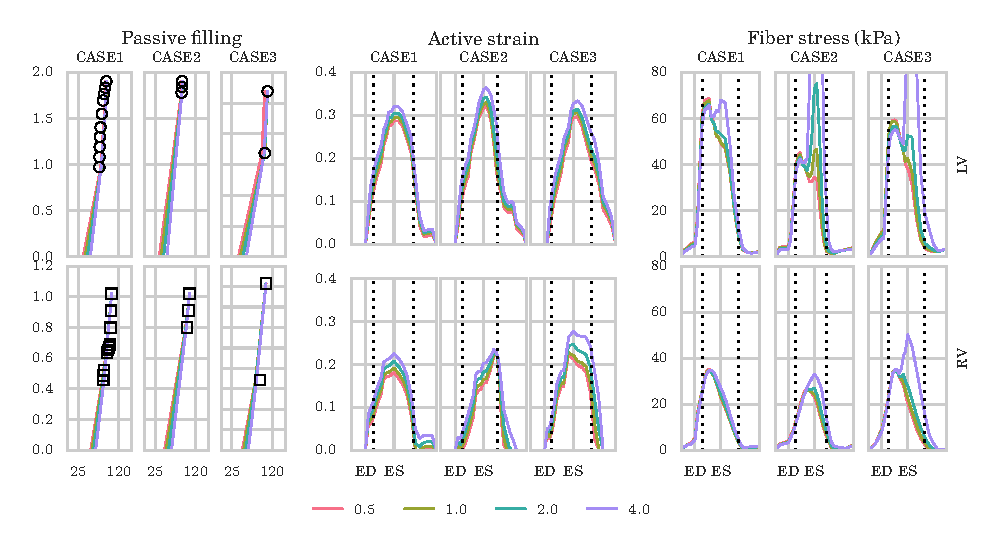
\includegraphics[width=\textwidth]{figures/startsens_results}
  \caption{\label{paper3:fig:startsens}To the left we show the passive
    filling curves, with volume in ml on the $x-$axis and pressure in
    kPa on the $y-$axis with different unloaded volume resulting from
    different material parameters used to estimate the unloaded
    geometries. Middle and right panel show average time traces of
    estimated active strain and Cauchy fiber stress respectively for
    different choice of unloaded configuration. Top row shows the
    results in the left ventricle while bottom row shows the results
    in the right ventricle. Here the values $a = 0.5, 1.0, 2.0$ and
    $4.0$ kPa are used to unload the ventricles. }
\end{figure}



\newpage
\bibliographystyle{plain}
\bibliography{chapters/paper3/bibliography}






\graphicspath{{chapters/paper4/}}


\chapter{Paper 4}
{\Huge \textbf{Assessment of regional myocardial work from a patient-specific
  cardiac mechanics model}}

% \clearpage
\newpage
\section*{Assessment of regional myocardial work from a patient-specific
  cardiac mechanics model}

% \begin{center}
  Henrik Finsberg$^{1,2,3}$,
  John Aalen$^{2,5}$,
  Camilla K. Larsen$^{2,5}$,
  Espen Remme$^{2,5}$,
  Joakim Sundnes$^{1,2,3}$,
  Otto A. Smiseth$^{2,5}$, and
  Samuel Wall$^{1,2,4}$,
% \end{center}

% \onehalfspacing
\footnotesize
\begin{enumerate}[itemsep=-2mm]
\item{Simula Research Laboratory, Lysaker, Norway}
\item{Center for Cardiological Innovation, Oslo, Norway}
\item{Department of Informatics, University of Oslo, Oslo, Norway}
\item{Department of Mathematical Science and Technology, NMBU, \r{A}s,
    Norway}
\item{Institute for Surgical Research, Oslo University Hospital, Oslo,
    Norway} 
\end{enumerate}
\normalsize
 

\subsection*{Abstract}
Subject-specific computational models of heart mechanics, calibrated
to replicate clinically measured motion data, can be used to estimate
regional myocardial work, and thereby provide a measure of regional
function and dysfunction. 

Finite element models of human left ventricles (LV) of one healthy
case and one patient diagnosed with left bundle branch block (LBBB)
were fitted to clinical data consisting of LV volume, regional
longitudinal strain, and non-invasive estimates of LV
pressure. Model-data mismatch was minimised using a gradient-based
optimization technique. Regional myocardial work was assessed using
several approaches, including the area of pressure-strain loops and
the area of fiber stress-strain loops. Qualitative indices of
efficiency and quantitative measures of mechanical power density were
compared using the different approaches, including the well
established pressure-volume area. 

The results show an excellent fit between measured and simulated
ventricular volumes and strains. The different methods to calculate
regional work are shown to be qualitatively similar, and they are all
able to capture regional dysfunction. However, the different
approaches are quantitatively very different, and the best agreement
between the sum of regional work contributions and the actual stroke
work is obtained using stresses and strains estimated with a finite
element model. In conclusion, mechanical work computed using a
personalized cardiac mechanics model is quantitatively similar to the
actual mechanical work estimated by the area of the pressure-volume
loop. This allows for potentially non-invasive quantitative assessment
of regional myocardial work, and would greatly improve diagnostics of
patients with regional dysfunction, such as dyssynchronous heart
failure.

\section{Introduction}



% Left ventricular (LV) systolic function is commonly quantified
% using global indices such as ejection fraction or QRS-width. However,
% these are global measures that does not take into account that regional
% dysfunction, such as dyssynchrony, might be present.

Patients suffering
from left ventricular dyssynchrony, such as in the 
case of left bundle branch block (LBBB), might experience an inefficient pumping
of blood due to uncoordinated contraction of different
segments in the heart. Cardiac Resynchronization Therapy (CRT) is
a well established treatment option for these patients \cite[Section
8.2]{ponikowski20162016}. However, 30-40 \% of patients selected for
this treatment do not respond positively, indicating that the current
selection criteria are sub-optimal, and that new biomarkers are needed
for improving the current clinical practice. 

Typically for LBBB is that septal segments are activated early,
causing a stretch of the opposing lateral wall. The 
contraction of the late-activated lateral wall then results in a 
lengthening of the septal segments during systole, which can be
identified as wasted work. Recent studies 
\cite{vecera2016wasted} have shown that wasted septal work due to the
uncoordinated contraction is a good predictor for response to
CRT, and that the amount of wasted work reflects the potential for
recovery. In these calculations, regional work is computed as the area
of the pressure-strain loops, where regional longitudinal strain is
measured using speckle tracking echocardiography (SPE), and left
ventricular pressure (LVP) is estimated using a non-invasive method
\cite{russell2012novel}. The same approach, though with other ways of
assessing regional strain and LVP, has been used in earlier studies to
quantify regional myocardial work
\cite{tyberg1974analysis,theroux1974regional}. These calculations are
inspired by the well established correlation between pressure-volume
(PV) area and myocardial oxygen consumption \cite{suga1979total}.
%  the
% area bounded by the end-systolic PV line, the systolic limb of the PV
% loop trajectory and the volume-axis,

% Total mechanical energy computed using a time-varying elastance model
% show strong correlation with cardiac oxygen consumption
% \cite{suga1979total}. Moreover, in the same study it was shown that
% under the assumtions stated in the time-varying elstance model, the
% energy consumtion of a real left ventricle was about twice as much as
% the total mechanical energy, suggesting that about 50 $\%$ of the
% energy is used for contractile purposes while the rest dissipate as
% heat.


Although the pressure-strain loop area as an estimate of regional
myocardial work has shown to be a useful metric in e.g predicting the
response to CRT, it suffers from limitations when compared to computation of 
``real'' myocardial work. Intraventricular pressure is
used as a surrogate for stress, because stress is not possible to
directly measure in an intact heart
\cite{huisman1980measurement}. Consequently, in these calculations all
segments are assumed to be subjected to the same stress, regardless of
differences in overall size, curvature or wall thickness.  
These limitations have been evaluated by Delhaas et. al
\cite{delhaas1994regional} who showed that
the area of regional fiber stress-strain loops was correlated to
regional oxygen demand in six canine left ventricles. In this study,
regional fiber stress was estimated based on assumptions of rotational
symmetry \cite{arts1991relation}, with each segment scaled according to
measured fiber strain. Fiber strain was measured at the subepicardial
layers using a two-dimensional video technique.
However, several simplifications, in particular regarding symmetry, is
made in these simplified models \cite{zhang2011comparison}, and the
measurement has to be done {\it in situ}.

Finite element models offer a safe and accurate way assessing
regional myocardial work {\it in vivo}, through mechanics models
constrained with clinical data \cite{balaban2017high}. This approach
allows for formulation of proper constitutive relations
\cite{holzapfel2009constitutive}, and realistic ventricular geometries
and fiber architecture. Hence, more realistic estimates of fiber
stress can be computed and fiber strain can be estimated through the
wall and are therefore not limited only to the subepicardial layers. 

% Approaches involving simple approximations of ventricular fiber or
% wall stress assumes symmetric properties of the left ventricle, and
% homogeneous distribution of fiber stress. These assumptions are vital
% in terms of stress estimation, and are known to cause
% discrepancy between stresses computed using Laplace-type laws and
% stresses computed in a finite element model
% \cite{zhang2011comparison}.


Wang et al \cite{wang2011myocardial} used displacements from
tagged MRI to estimate a single set of material parameters and a
time-varying active tension in a finite element model of five
canine left ventricles. These parameterized models were used to assess
regional myocardial work using an approach outlined in
\cite{niederer2009role}, and they found large regional variations.

A framework for assessing regional estimates of myocardial
work, for which, when all regions are considered, sums up to the total
stroke work needed to eject blood to the body, is still
lacking. Furthermore, in order to be clinically useful, the framework
has to be accurate in terms of being able to replicate the mechanical
conditions observed clinically, and fast in terms of computing these
estimates within a reasonable time frame.

In this study we apply a recently developed framework
\cite{balaban2017high} for constraining a mechanical model to clinical
data. This framework employs gradient-based optimization to estimate high
dimensional parameters in order to minimize the model-data
mismatch. Moreover, the framework utilizes state-of-the-art numerical
methods which computes the gradient efficiently by solving the
corresponding adjoint equation, and thereby provides these estimates
within a reasonable time frame.  

The result is a personalized cardiac mechanics model, that can used to quantify
regional myocardial work. We perform both a qualitative and a
quantitative analysis of the different methodologies to asses regional
as well as global measures of work. In particular we compare work
computed using a finite element model, with work computed as the area
of the pressure strain-loops, and also compare these results
to the total stroke work estimated by the area of the
pressure-volume loop.



\section{Methods}


\subsection{Mechanical modeling}
\label{paper4:sec:mechanical_modeling}
We represent the heart as a continuum body with a reference configuration 
$\Omega \subset \mathbb{R}^3$, and let $\Xvec$ denote the
corresponding reference coordinate. Further let $ \Omega_t
\subset \mathbb{R}^3$ be the deformed domain after a given time $t >
0$ and let $\xvec$ be the corresponding physical coordinate.  The
motion of a point $\Xvec \in  \Omega$ to the  point $\xvec \in
\Omega_t$ may be described by a deformation map  $\varphi :
\Omega  \rightarrow \Omega_t$. 

The deformation gradient associated with the motion $\xvec =
\varphi(\Xvec)$ is a rank-2 tensor given by 
\begin{align}
\F(\Xvec) = \frac{\partial \varphi}{\partial \Xvec},
\end{align}
and the deformed and reference configuration are related via the
displacement field  $\uvec$ by 
\begin{align}  
\uvec = \xvec-\Xvec = \varphi( \Xvec) -\Xvec.
\end{align}
Further, we introduce the determinant of the deformation gradient, $J =
\det \F$, and the right Cauchy-Green deformation tensor $\C = \F^T \F$.

The myocardium is modeled as a hyperelastic material, and we adapt a
transversely isotropic law from \cite{holzapfel2009constitutive},
where the strain-energy function $\Psi$ is given by  
\begin{align}
  \label{paper4:eq:hoa}
  \Psi(\Cbar) = \frac{a}{2 b} \left( e^{ b (\bar{I}_1  - 3)}  -1 \right)
  + \frac{a_f}{2 b_f} \left( e^{ b_f (\bar{I}_{4\ef} - 1)_+^2} -1 \right). 
\end{align}
Here $\bar{I}_1 = \tr \Cbar$ and $\bar{I}_{4\ef}= \ef \cdot (\Cbar
\ef)$ with $\Cbar = J^{-2/3}\C$ being the isochoric part of the right
Cauchy-Green deformation tensor , $\ef$ is a
unit vector field in the direction of the myofibers, $(\cdotp)_{+} 
= \max\{\cdot, 0\}$, and $a, a_f, b, b_f$ are 
material stiffness parameters defining the elastic properties of the
myocardium.

Incompressibility is enforced by using a two-field variational approach
where the term
\begin{align}
\Psi_{\text{vol}} = - p (J-1), 
\end{align}
is added to the total strain energy density, and the variable $p$ is
introduced as a Lagrange multiplier.

To model the active contraction of the ventricle we employ the active
strain formulation. In this formulation one assumes a multiplicative 
decomposition of the deformation gradient into an elastic
and an active component \cite{ambrosi2011electromechanical}:
\begin{equation}
 \F = \F_e \F_a.
\label{paper4:eq:active_strain}
\end{equation}
The active part, $\F_a$ represents the active shortening of the cells,
while the elastic part $\F_e$ ensures compatibility of the tissue.
Similar to \cite{balaban2017high} we choose the following form of the active
deformation gradient,
\begin{equation}
  \F_a = (1 - \gamma) \ef \otimes \ef  + \frac{1}{\sqrt{1 - \gamma}} (\I - \ef \otimes \ef).
 \label{paper4:eq:active_strain_Fa_gjerald}
\end{equation}
The active deformation gradient $\F_a$ does not contribute to any
stored energy within the material, so that the modified
strain-energy function $\tilde{\Psi}(\C_e) = \Psi(\F_a^{-T} \Cbar
\F_a^{-1})$, which is a pure function of the elastic deformations is used.

The force balance equation can be derived from the classical Cauchy
momentum equation, and with the assumption that the inertial term and
external body forces are negligible, the strong formulation yields
\begin{align}
  \nabla \cdot \FPiola &= 0, \\
  J &= 1, 
\end{align}
with $\FPiola = \frac{\partial \Psi}{\partial \F}$ being the first
Piola-Kirchhoff stress tensor. 

To solve the problem we employ the Galerkin finite element method, which is based
on choosing proper finite dimensional subspaces $V_h \subset [H_0^1(\Omega)]^3$ and
$Q_h \subset L^2(\Omega)$ and solve the weak formulation of the problem. In
the Lagrangian form, the weak form reads: {\it find $(\uvec,p)
\in V_h\times Q_h$ such that for all variations $(\delta
\uvec, \delta p) \in V_h \times Q_h $ and $\left. \left( \uvec \cdot \N \right)
\right|_{\partial \Omega_{\mathrm{base}}} = 0$ }:
\begin{align}
\begin{split}
  F(\uvec, p;\delta \uvec, \delta p) =
  &\int_{\Omega} \FPiola :  \Grad \delta \uvec  \mathrm{d} V  \\
  &+\int_{\Omega} p J \F^{-T} : \Grad \ \delta \uvec   \mathrm{d} V  
  +\int_{\Omega} (J - 1) \delta p \mathrm{d} V \\
  &+\int_{\partial \Omega_{\text{base}}} k \uvec \cdot \N \mathrm{d}S
  - \int_{\partial \Omega_{\text{endo}}} \plv J \F^{-T} \N \cdot \delta \uvec \mathrm{d}S= 0.
  \label{paper4:eq:force_balance}
\end{split}
\end{align}
Here, the ventricular domain is anchored by constraining the basal
motion by a linear spring-term with stiffness $k$, and the
endocardial cavity pressure $\plv$ is enforced as a Neumann boundary
condition on the endocardium.  

For discretization we use the so called Taylor-Hood finite elements,
which is known to yield a stable discretization for this problem
\cite{arnold1984stable}. These elements consist of quadratic finite
elements for the displacement, and linear finite elements for
the hydrostatic pressure. 



\subsection{Calculation of work}
\label{paper4:sec:regional_work}

Work can be computed by considering any of the
work conjugate stress-strain pairs \cite{holzapfel2000nonlinear}. In
the current configuration it is common to use the Cauchy stress tensor
$\Cauchy = \FPiola \F^T$ and the Almansi strain tensor $\mathbf{b} =
\frac{1}{2} \left(\I -  \F^{-T} \F^{-1} \right)$, while in
the reference configuration we use the second Piola-Kirchhoff stress
tensor $\SPiola = \F^{-1} \FPiola$, and the Green-Lagrange strain
tensor $\E = \frac{1}{2}\left(\C - \I \right)$. Thus, in the Lagrangian
description, the total mechanical work from time $t_1$ to $t_2$ in a
region $\Omega_j$ is given by
\begin{align}
   \mathcal{W}(t_1, t_2)[\Omega_j] = 
  -\int_{t_1}^{t_2} \int_{\Omega_j}\SPiola(t, \Xvec)
  : \dot{\E}(t, \Xvec) \mathrm{d}\Xvec \mathrm{d}t, 
\end{align}
where $ \dot{\E} $ is the rate of the Green-Lagrange strain tensor.
By dividing by the volume of the region of interest $| \Omega_j |$,
we obtain the average work density in that region. Note that the sign
convention used here implies that a negative strain-rate
represents positive work. To only compute the
work along a specific direction, e.g  work done by normal stress along the fibers, the full stress
and strain tensors are simply interchanged with their respective
components in that direction, and the double contraction of the tensors
is changed to a scalar multiplication.

The mechanical work needed to eject blood from time $t_1$ to
$t_2$ is given by
\begin{align}
   \mathcal{W}(t_1, t_2)[\Omega] = 
  -\int_{t_1}^{t_2} \frac{\mathrm{d}V}{\mathrm{d}t} P(t) \mathrm{d}t,
\end{align}
where $V(t)$ and $P(t)$ refers respectively to the cavity volume and pressure in
the left ventricle $\Omega$ at time $t$. If the $t_1$ and $t_2$
represent, respectively, the start and end of the cycle, then normalizing with respect to the
total ventricular wall volume  $| \Omega |$, yields a measure of
total mechanical work density (TMWD). Diving the TMWD by the total
cycle time, yields a measure of total mechanical power
density (TMPD). We note that for analysis of performance, TMPD is
a better measure than total work because it is independent of
morphology and heart rate.  

\subsubsection{Quasi-static approximation}
The mechanical model described in Section
\ref{paper4:sec:mechanical_modeling} is quasi-static, meaning that the
inertial forces are assumed to be so small that the
equilibrium equation \eqref{paper4:eq:force_balance} holds at any discrete
time point. Therefore, strain rate is estimated using a
backward difference approximation \cite{wang2011myocardial}.
Suppose we have $N+1$ discrete time points $t_i, i = 0,1, \cdots N$, where $ t_0$
refers to the the reference configuration, and let $\SPiola(t, \Xvec)$
and $\E(t, \Xvec)$ be respectively the stress and strain tensors at
time $t$ and position $\Xvec$ in the reference configuration. In the
following, the full stress and strain tensors are used, but the methodology
also applies to any component of the stress and strain tensor. We define
\begin{align}
  \overline{\SPiola}(t_i,\Xvec) &= \frac{1}{2}\left( \mathbf{S}(t_i,\Xvec) + \mathbf{S}(t_{i-1},\Xvec) \right),\\
  d\E(t_i,\Xvec) &= \E(t_i,\Xvec) - \E(t_{i-1},\Xvec),
\end{align}
for $i = 1,\cdots, N$, and note that $ \mathbf{S}(t_0) = \mathbf{E}(t_0) = \mathbf{0}$.
The mechanical work in a region $\Omega_j$ from time $t_m$ to time $t_n$ can now be approximated
as 
\begin{align}
  \begin{split}
   \mathcal{W}(t_m, t_n)[\Omega_j]
  &= -\int_{t_m}^{t_n} \int_{\Omega_j}\SPiola(t, \Xvec) : \dot{\E}(t, \Xvec) \mathrm{d}\Xvec \mathrm{d}t \\
  &\approx - \sum_{i = m}^{n}\int_{\Omega_j}\overline{\SPiola}(t_i, \Xvec) : d\E(t_i, \Xvec) \mathrm{d}\Xvec
  \end{split}
\label{paper4:eq:total_work}
\end{align}
Similarly, the mechanical work computed from the pressure-volume loop area can be estimated as  
\begin{align}
  \begin{split}
  \mathcal{W}(t_m,t_n)[\Omega]
  &= - \int_{t_m}^{t_n} \frac{\mathrm{d}V}{\mathrm{d}t} P(t) \mathrm{d}t \\
  &\approx -\sum_{i= m}^{n}  (V(t_i) - V(t_{i-1})) \cdot \frac{P(t_i) + P(t_{i-1})}{2}.
  \end{split}
\end{align}

\subsubsection{Efficiency and wasted work ratio (WWR)}
\label{paper4:sec:efficiency_wwr}

During systole, most segments shorten and perform positive work
($\mathcal{W}_{\mathrm{pos}}$). However some segments might elongate,
resulting in energy loss, and we say that these segments do negative work
($\mathcal{W}_{\mathrm{neg}}$). Positive work is identified as the points with
$d\E_{\ef}(t) < 0$ (shortening), while negative work is identified as points with
$d\E_{\ef}(t) > 0$ (lengthening).
A local measure of the energetic efficacy of each segment is the ratio between the
negative and positive work, an index known as the segmental wasted
work ratio (WWR) \cite{russell2013assessment},
\begin{align}
  \mathrm{WWR} = \frac{|\mathcal{W}_{\mathrm{neg}}|}{\mathcal{W}_{\mathrm{pos}}}
\end{align}
Another measure of efficiency, formulated by Niederer et al
\cite{niederer2009role} is the ratio of positive work and the total
work
\begin{align}
  \eta = \frac{\mathcal{W}_{\mathrm{pos}}}{\mathcal{W}_{\mathrm{pos}} + |\mathcal{W}_{\mathrm{neg}}|}.
  \label{paper4:eq:efficiency}
\end{align}

The two indices are related by $\eta = \left( 1 +
  \mathrm{WWR} \right)^{-1}$, and we will therefore only report values
of the efficiency \eqref{paper4:eq:efficiency}, for which a value close to 1.0 indicate that most
of the performed work is positive. Since we expect work during systole
to be the main contribution to the overall ejection of blood, the
index is computed by only including work done from mitral valve closing to
mitral valve opening \cite{russell2013assessment}. 

% Note that with the current sign-convention, negative work is by
% definition negative, which is why we take the absolute value of the
% negative work. 

\subsection{Pre-processing of in vivo data sets}

In this study 4D echocardiographic images of one patient diagnosed
with left bundle branch block (LBBB) and one healthy volunteer was
acquired using a GE Vingmed E9 machine (GE Healthcare Vingmed, Horten,
Norway). 
The analysis of the echocardiographic images was conducted with the
GE software package EchoPac version 202. Longitudinal strain was
measured via speckle tracking echocardiography (SPE) in the 17 AHA segments
\cite{cerqueira2002standardized}. However, the apical segments for both
subjects, as well as the inferior and posterior basal segment for the
normal case, were excluded due to poor quality.

Using a semi-automatic image segmentation tool, the LV cavity volumes for
each frame was measured, and the LV endocardial and epicardial
surfaces were extracted from the image frame corresponding to
beginning of atrial systole \cite{hansegaard2009semi}. A cut was made
at the base of these surfaces so that the measured and computed cavity
volumes agreed within a tolerance of 1 ml. Thereafter, a left
ventricular tetrahedral mesh was created using Gmsh
\cite{geuzaine2009gmsh}. Myocardial fiber orientations were assigned
using the Laplace-Dirichlet Rule Based  (LDRB) algorithm
\cite{bayer2012novel} with an angle of $60^{\circ}$ on the endocardial
and $-60^{\circ}$ on the epicardial surface
\cite{streeter1969fiber}. A non-invasive method
\cite{russell2012novel} was used to estimate an LV pressure curve for
both subjects, so that all clinical data used in this study were
acquired using non-invasive methods. 


\subsection{Data assimilation and parameter estimation}

In order to constrain the mechanical model to clinical data, we
applied a variational data assimilation technique. Let $\mathbf{w} =
(\uvec,p)$ denote a joint state variable consisting of the
displacement field $\uvec$ and the hydrostatic pressure $p$. The LV
cavity volume can be approximated as  
\begin{align}
  \mathcal{H}_{\mathrm{volume}}(\mathbf{w})= -\frac{1}{3}\int_{\lvendo}
  \left( \Xvec + \uvec \right) J \F^{-T} \Nvec \mathrm{d}S, 
  \label{paper4:eq:volume_operator}
\end{align}
where $\N$ denotes the unit facet normal. Furthermore, the average regional
longitudinal strain can be approximated in region number $j$ as
\begin{align}
  \mathcal{H}_{\mathrm{strain}, j}(\mathbf{w}) = \frac{1}{|\Omega_j|}\int_{\Omega_j}
  \mathbf{e}_l^T \left( \mathbf{\tilde{\F} - \I} \right)\mathbf{e}_l  \mathrm{d}V.
\end{align}
Here $\mathbf{e}_l$ denotes a unit vector field in
the longitudinal direction, and $\tilde{\F}$ refers to the modified deformation
gradient relative to the reference geometry in the measurements. 

For a given measurement $y_k$, we want to find a state variable
$\mathbf{w}$ that minimizes the mismatch between $y_k$ and
$\mathcal{H}_k(\mathbf{w})$. The state variable is determined by
tuning model-based parameters, also
referred to as control parameters, which we generically denote
by $\mu$. This can be formulated as a PDE-constrained optimization
problem of the form
\begin{equation}
  \begin{aligned}
    \label{paper4:eq:pde_opt}
    & \underset{\mu}{\text{minimize}}
    & &  \mathcal{J}(\mathbf{w}(\mu), \mu) \\
    & \text{subject to}
    & & F(\mathbf{w}, \mu)  = 0,
  \end{aligned}
\end{equation}
where $F=0$ represents the PDE-constraint given by
\eqref{paper4:eq:force_balance}, and $\mathcal{J}$ is a possibly
multiobjective function  
\begin{align}
  \mathcal{J}(\mathbf{w}(\mu), \mu) = \sum_{k = 1}^{N} w_k j_k (\mathbf{w}(\mu), \mu),
  \label{paper4:eq:cost_functional}
\end{align}
with $w_k$ being scalar weights, and $j_k = d( y_k,
  \mathcal{H}_k(\mathbf{w}) ) $ for some suitable metric $d$.



\subsubsection{Joint estimation of unloaded configuration and passive
  material parameters}
\label{paper4:sec:passive_param_estim}

One challenge when using image-based geometries is that the geometry
observed in a medical image is subjected to loads, e.g blood
pressure, while our finite element formulation assumes a stress-free
reference configuration. Therefore we need to find a geometry, so
that when the measured pressure in the image is applied, we recover
the image-based geometry. Several methods for estimating the unloaded,
zero-pressure geometry exist, including the inverse design analysis
(ID) \cite{govindjee1996computational}, the modified updated
Lagrangian formulation (MULF) \cite{gee2010computational} and
iterative methods \cite{bols2013computational,Rausch2017JB}.
Here we apply a simple fixed-point iteration scheme known as the backward
displacement method \cite{bols2013computational}.
The estimated unloaded configuration will depend upon the choice of material
parameters, which is not know  \emph{a priori}. In Appendix
\ref{paper4:sec:unloading} we explain the main steps in the backward
displacement method and a proposed method for joint estimation of material
parameters unloaded configuration. Additionally, an analysis of
the convergence properties of this method is also provided.


\subsubsection{Active parameter estimation}
\label{paper4:sec:active_param_estim}
From the first measurement point after end-diastole and throughout the
remaining cardiac cycle, that parameter $\gamma$ in
\eqref{paper4:eq:active_strain_Fa_gjerald} is used as control in
\eqref{paper4:eq:pde_opt}, and the cost functional \eqref{paper4:eq:cost_functional}
at time point $i$ is given by 
\begin{align}
  \mathcal{J} =
   \left(\frac{\mathcal{H}_{\mathrm{volume}}(\uvec^i)
  - V^i}{V^i} \right)^2 +
  \sum_{j=1}^{12} \delta_j \left( \mathcal{H}_{\mathrm{strain}, j}(\uvec^i)
  - \varepsilon_{j}^i \right)^2  + \lambda \| \nabla \gamma \|^2.
\end{align}
Here $V^i$ is the measured cavity volume at time point $i$, 
$\varepsilon_{j}^i$ is the measured longitudinal strain in segment $j$
at time point $i$, and $\delta_j$ is 0 if the measurement in segment
$j$ is missing and 1 otherwise. Note that even though the  
AHA-representation \cite{cerqueira2002standardized} contains 17
segments, we only include the mid and basal segments in the
optimization because of the relatively poor quality of the apical
segments, leaving us with a total of 12 segments.

The parameter $\gamma$ is represented as a piecewise linear function
with one parameter per vertex as suggested in \cite{balaban2017high}.
This problem is therefore highly under-constrained, meaning that there
are potentially many solutions to problem. To remedy this we apply a
Tikhonov regularization, where we penalize non-smooth values of the
control by adding the term $\lambda \| \nabla \gamma \|^2$ to the
objective functional. The regularization parameter $\lambda$
was chosen based on a previous study to be $\lambda=0.01$ \cite{balaban2017high}.

The initial guesses for the optimization in this phase were set to
zero in the first iteration, and in subsequent iterations, the initial
guesses were set to the optimized values found in the previous iteration.

\section{Results}
For the normal and LBBB case described above, we ran the
full data assimilation pipeline on two meshes, where one was a refined version of the
other. For the normal case, the original and refined mesh had
respectively 2569 and 5258 elements, while the LBBB case
had 2572 elements in the original mesh and 5114 elements in the
refined mesh. Results on the original and refined geometries gave
close to identical results, and we will therefore only present the
results using the coarsest geometry. 

All simulations were carried out using an in-house software
package\footnote{Source code is publicly available at
  \url{https://bitbucket.org/finsberg/pulse_adjoint}} 
based on FEniCS \cite{logg2012automated} and Dolfin-Adjoint \cite{farrell2013automated}.
In these simulations the value of the linear spring $k$ in
\eqref{paper4:eq:force_balance} was determined by testing a range of values,
and choosing the softest spring that allowed for a convergent
estimation of the unloaded configuration. Based on this experiment we
choose $k=0.01$ kPa/cm$^2$.

During the estimation of the active and passive parameters outlined in Section
\ref{paper4:sec:active_param_estim} and \ref{paper4:sec:passive_param_estim}
respectively, the optimization was terminated if the difference between two
successive iterations was less then $10^{-6}$ or the number of
iterations exceeded 100. For the material parameter, an upper and lower
bound was set to $50$ and $0.05$ kPa respectively, while for the active
parameter these bounds were set to $0.4$ and $0.0$, allowing for up to
40 $\%$ active shortening of the myofibers. 



% \subsection{Estimation of unloaded configuration and passive material
%   parameters}

% The linear isotropic material parameter $a$ in \eqref{paper4:eq:hoa}, along
% with an unloaded configuration was estimated by means of Algorithm
% \ref{paper4:alg:unload_mat_bdm} for both the normal and the LBBB case.
% Figure \ref{paper4:fig:unloaded_simulation} shows the value of the material
% parameters, and the residual representing the relative difference
% between the unloaded cavity volumes of two successive iterations.
% The LBBB and normal case used respectively
% $7$ and $17$ iterations to get the residual below 0.01, resulting in a
% material parameters of $a= 32.1$ kPa for the LBBB case and $a= 11.96$ kPa for the
% normal case.
% \begin{figure}[htbp]
%   \centering
%   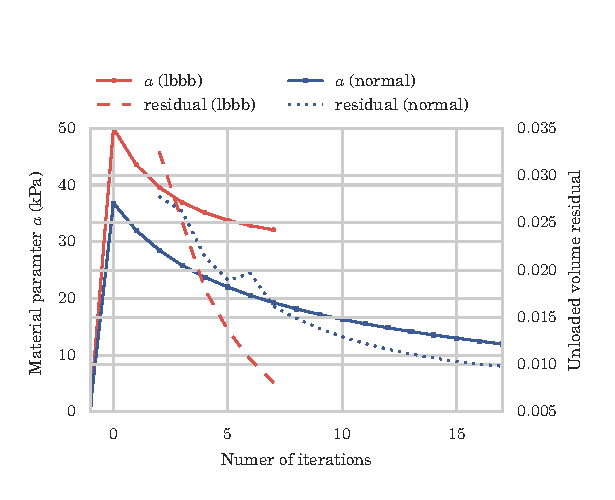
\includegraphics{figures/unloaded_simulation}
%   \caption{\label{paper4:fig:unloaded_simulation}Estimation of material
%     parameters for normal (blue) and LBBB (red) case. Solid lines
%     show the value of the material parameter at each iteration with
%   initial guess in both cases being $a=1.291$ kPa (iteration -1). Then
% the offset of the pressure in the image-based geometry was subtracted
% and new material parameters was estimated (iteration 0), and Algorithm
% \ref{paper4:alg:unload_mat_bdm} was applied using this estimate as initial
% guess. Dashed lines are the residuals, representing the relative
% difference in unloaded cavity volume. The algorithm terminated when
% the residual was below 1 \%. }
% \end{figure}
% Figure \ref{paper4:fig:unloaded_geo} shows the resulting
% unloaded configurations on top of the original geometries. 
% \begin{figure}[htbp]
%   \centering
%   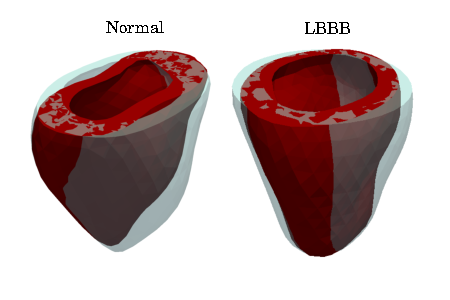
\includegraphics{figures/unloading}
%   \caption{\label{paper4:fig:unloaded_geo}Estimated unloaded
%     configuration for normal (right) and LBBB (left) case in red, and
%     the original image-based geometry in transparent. }
% \end{figure}


\subsection{Data assimilation}

The simulated and measured PV loops and the regional
pressure-strain loops are shown in Figure \ref{paper4:fig:pv_loops} and
\ref{paper4:fig:regional_strain_pressure_loops} respectively. 
For the normal case, the longitudinal strain curves in the basal
inferior and posterior segments were missing, and so only the
simulated results are shown in these segments.

\begin{figure}[htbp]
  \centering
  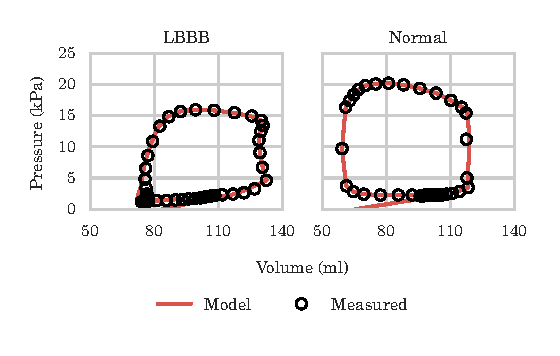
\includegraphics{figures/pv_loop}
  \caption{\label{paper4:fig:pv_loops}Simulated and measured PV loops
    for the LBBB (left) and normal (right) case. }
\end{figure}

In both the normal and the LBBB case, the
largest deviation between the measured and simulated volumes were found
during the end of isovolumic relaxation, where simulated volumes were
respectively at most 1.0 and 6.0 ml lower than the measured volumes.


\begin{figure}[htbp]
  \centering
  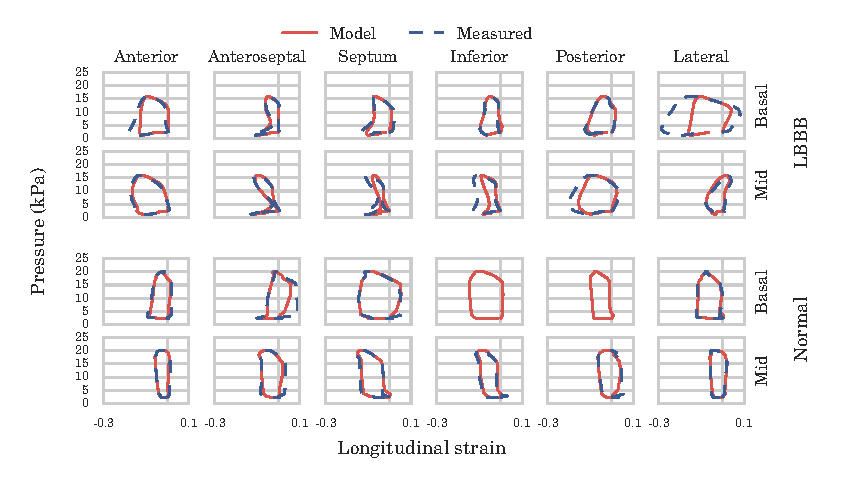
\includegraphics{figures/pressure_strain_loop}
\caption{\label{paper4:fig:regional_strain_pressure_loops}Measured and
simulated pressure-strain loops for LBBB (top) and normal (bottom)
case. Strain measurement in basal inferior and posterior segments for
the normal subject were discarded in the optimization due to poor
quality, and therefore only simulated results are shown in these
segments.} 
\end{figure}



\subsection{Estimation of regional myocardial work}

Analogous to the regional pressure-strain loops in Figure
\ref{paper4:fig:regional_strain_pressure_loops}, the resulting regional fiber
stress-strain loops are depicted in Figure
\ref{paper4:fig:regional_fiber_stress_strain_loops}. Here we show Cauchy
fiber stress on the $y-$axis and for the sake of correct illustration
of regional work in terms of loop area, we show the Almansi fiber
strain on the $x-$axis. 

\begin{figure}[htbp]
  \centering
  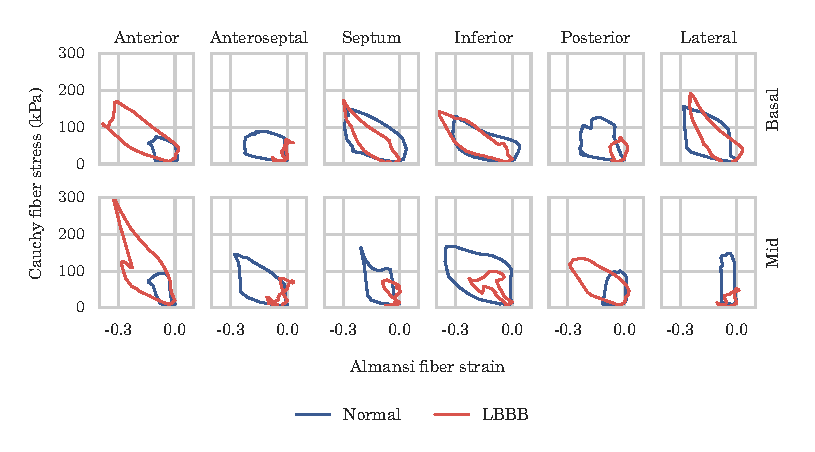
\includegraphics{figures/fiber_stress_strain_loop}
  \caption{\label{paper4:fig:regional_fiber_stress_strain_loops}Simulated
    regional fiber stress-strain loops in the mid and basal segments
    for normal (blue) and LBBB (red). } 
\end{figure}

The Cauchy fiber stress visualized at the deformed configurations at
the different valvular events for the normal and LBBB case are shown
in Figure \ref{paper4:fig:snap_shots}. The LBBB case shows clear signs of
dyssynchrony and more uneven distribution of stress compared to the
normal case. 

\begin{figure}[htbp]
  \centering
  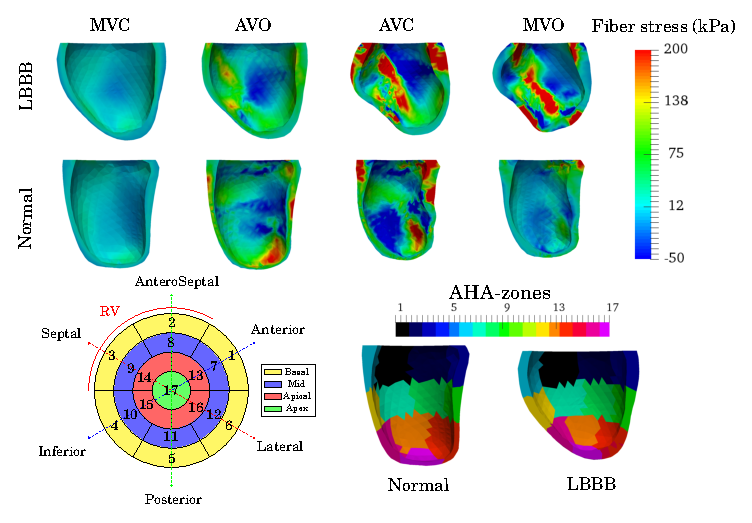
\includegraphics{figures/snap_shots}
  \caption{\label{paper4:fig:snap_shots}Cauchy fiber stress for the normal and LBBB case at
    different valvular events (MVC: mitral valve closing, AVO: aortic
    valve opening, AVC: aortic valve closing, MVO: mitral valve
    opening), visualized on the deformed configurations. For reference
    we show the 17 AHA-zone delineation of the left ventricle in the
    two cases in the bottom panel. From left to right we have the
    lateral, anterior, anteroseptal and septal segments. }
\end{figure}




The total mechanical power density (TMPD) is also computed using four
different approaches: 1) area of the pressure-volume loop normalized
to ventricular wall volume, 2) using the full stress and strain tensors,
3) using the fiber component of the stress and strain tensors, and 4)
using global longitudinal strain and estimated pressure. Table
\ref{paper4:tab:total_mechanical_power} show these values for the two
subjects, in units kW m$^{-3}$. In the calculations of pressure volume
area, the simulated volume is used, with the unloaded volume and zero
pressure included as reference point.

\begin{table}
\caption{Total mechanical power density (TMPD) computed using the area
  of the pressure-volume loop normalized to ventricular wall volume
  (PV area), the full stress and strain tensors (Full), the fiber
  component of the stress and strain tensors (Fiber) and using global
  longitudinal strain and estimated pressure (Pressure-GLS)} 
\begin{tabular}{lrrrr}
\hline
 Case   &   PV area (kW m$^{-3}$) &   Full (kW m$^{-3}$) &   Fiber (kW m$^{-3}$) &   Pressure-GLS (kW m$^{-3}$) \\
\hline
 LBBB   &                    8.41 &                10.60 &                  6.42 &                         1.02 \\
 Normal &                   15.79 &                16.35 &                  9.59 &                         1.59 \\
\hline
\end{tabular}
\label{paper4:tab:total_mechanical_power}
\end{table}

The regional TMPD, computed using the fiber
component of the stress and strain tensor, is illustrated for the mid
segments for the two subjects in Figure
\ref{paper4:fig:regional_power_density}. These regional values are
effectively the area of the fiber stress-strain loops in Figure
\ref{paper4:fig:regional_fiber_stress_strain_loops} normalized to cycle
time, in which the area is positive when the loop follows an
anti-clockwise orientation and negative if the loop has a clockwise
orientation. Regional TMPD using the full stress and strain tensor are
not shown, but were qualitatively similar to the regional TMPD using
only the fiber component.


\begin{figure}[htbp]
  \centering
  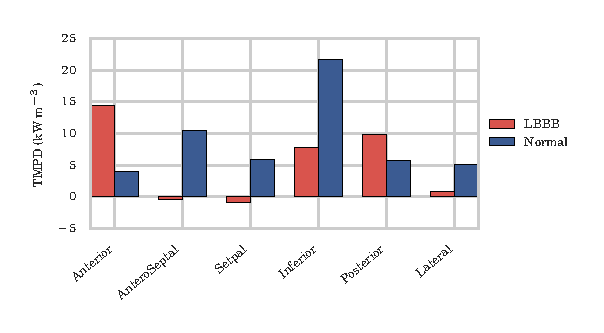
\includegraphics{figures/regional_power_density}
  \caption{\label{paper4:fig:regional_power_density} Regional TMPD in the mid
    segments for LBBB (left) and normal (right), computed using the
    fiber component of stress and strain tensors. Height of each bar
    indicate the area of the respective fiber stress-strain loop
    traversed in an anti-clockwise orientation, and normalized to
    cycle time.}  
\end{figure}

A qualitative comparison of the pressure-strain loops and fiber
stress-strain loops are illustrated in Figure
\ref{paper4:fig:regional_work_indices}, where we plot the regional efficiency
\eqref{paper4:eq:efficiency} using the two measures of work. We note that the
efficiencies computed using the fiber stress-strain loops are
lower than for the pressure-strain loops, but show the same trend, i.e
that regions with reduced efficiency coincide.  

\begin{figure}[htbp]
  \centering
  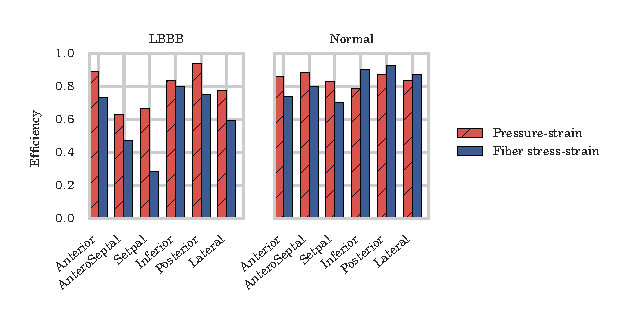
\includegraphics{figures/regional_work_indices}
  \caption{\label{paper4:fig:regional_work_indices} Regional efficiency in
    the mid segments computed according to \eqref{paper4:eq:efficiency} for LBBB (left) and normal (right)
    case. Red bars show efficiency based on areas of the pressure
    strain loops while blue bars show efficiency based on areas of the
    fiber stress-strain loops.}
\end{figure}


% \input{result_figures}
\section{Discussion}
In the present study, we have demonstrated how computational cardiac
modeling and data assimilation can be used to asses regional
myocardial work. The in vivo data sets making up these results are
based on echocardiographic images and non-invasive estimates of LV
pressure in one patient diagnosed with LBBB and one healthy volunteer. 
A gradient-based optimization method was used to minimize the mismatch
between the simulated and observed clinical data, so that the simulated
longitudinal strain and volume were quantitatively similar to the
measured values.

% In both cases an excellent fit of the PV loops was
% obtained, as can be seen in Figure \ref{paper4:fig:pv_loops}. The deviation
% between simulated and measured volume during late isovolumic
% relaxation shows that there is a trade-off between fitting both the
% strain and volume data. This can also be seen from the matching of the
% pressure-strain loops in Figure
% \ref{paper4:fig:regional_strain_pressure_loops}, where it is clear the some
% segments (e.g mid posterior and basal lateral) for the LBBB patient
% does not match exactly during the isovolumic relaxation phase. Whether
% this is a result of lack of mode fidelity, poor data compatibility, or
% just noise in the measurements is difficult to say.



\subsection{Pressure-strain versus fiber stress-strain}

The total mechanical work can be computed by considering the work done
by all segments during one full cardiac cycle. Ideally, we would have
a regional measure so that adding together all regional contributions
would sum up to the actual stroke work needed to eject blood to the
body. Since the stroke work is strongly correlated with the myocardial
oxygen consumption \cite{suga1979total}, a regional meausure of work
that summed up to the total stroke work would be a good measure of
regional performance. 
% Total mechanical power density (TMPD),
% which is a measure of average total mechanical work normalized to
% cycle time, is presented in Table
% \ref{paper4:tab:total_mechanical_power} using four different approaches,
% namely, the PV area, the full stress and strain tensor, the fiber
% stress-strain loops and the pressure-strain loops.

The TMPD computed using the PV area, which is a true measure of stroke
work, falls between the values of TMPD computed using the full stress
and strain tensor and the TMPD computed using the fiber stress and
fiber strain. In other words, the amount of work needed to eject blood
to complete a cycle is greater that the amount of work done by the
myofibers, but bounded above by the total mechanical work. Since there
are no viscous terms in the model, the energy should be
conserved. However, energy loss due work against the basal boundary
constraint could explain the difference between stroke work and the
total mechanical work. Furthermore, the TMPD computed from fiber
stress-strain area here, are comparable with values in other studies
using canine left ventricles \cite{delhaas1994regional}, which reports
values of TMPD in the range from 0.5 to 12.5 kW m$^{-3}$. Note that
TMPD is a measure that is independent of morphology, i.e size of the
ventricle and heart rate, and therefore reflect the actual performance.

The values in Table \ref{paper4:tab:total_mechanical_power} indicate that the
total mechanical work performed in the direction of the fibers is
approximately 60 $\%$ of the 
total mechanical work computed by taking into account the full stress
and strain tensor (LBBB: 60.5 $\%$, normal:58.7 $\%$). Of course, the
amount of work performed in transverse direction of the fibers will depend upon the
chosen form of the active deformation gradient in
\eqref{paper4:eq:active_strain_Fa_gjerald}. In the active stress approach on 
the other hand, where the total Cauchy stress tensor is additively decomposed into
active and passive contributions, it is common to add an active stress
in the transverse direction, which is also reported
experimentally \cite{lin1998multiaxial}. By assuming
a volume preserving active deformation gradient, the amount of
work in the cross fiber direction as computed here is about $40 \%$, a
value that has been used in other modeling studies using the active
stress approach \cite{sun2009computationally}.

The values of regional TMPD in the mid segments presented
in Figure \ref{paper4:fig:regional_power_density} show that the septal
segments for the LBBB patient actually consume energy and yield a
negative TMPD. On the other hand, the healthy heart shows positive TMPD
in all segments and generally higher values than the LBBB heart.
Since the TMPD computed using stress and strain derived from the
underlying constitutive equation agrees very well with the TMPD
computed from the PV area there is reason to believe that the regional
TMPD reflects the actual regional performance, and future studies should
investigate how well these values correlate with regional myocardial
oxygen consumption. 

The TMPD computed using the pressure and global longitudinal strain
only accounts for a small fraction of the total mechanical power.
This indicates that quantitatively this is not a good measure of
myocardial work. However, the area of the pressure-strain loops have shown to be a good metric
of regional efficiency and a promising index for predicting response
to CRT \cite{vecera2016wasted}. From Figure
\ref{paper4:fig:regional_work_indices} we see the same trends in terms of efficiency and wasted
work can be seen regardless of how work is computed, namely that early
activated segments are less efficient and have a higher wasted work
ratio than the other segments for the LBBB case. Therefore, relative
comparison of segments using pressure-strain loops seems to give the
same picture as when using the fiber stress-strain loops. 
The pressure strain loops for the LBBB case all have an
anti-clockwise orientation, indicating generation of work in all
segments. On the other hand, the fiber stress-strain loops in the
septal segments show a clockwise orientation which is evidence of
work usage. In other words, the two approaches show the same
trend, but the effect of the wasted work is magnified in the fiber
stress-strain loops.  

% The presence of clockwise oriented loops is primarily due to the change
% from longitudinal strain to fiber strain, and not the change from
% pressure to fiber stress. Therefore the re

% Myocardial fiber architecture is more or less longitudinally oriented
% near the subepicardial and subendocardial layers
% \cite{streeter1969fiber}, and therefore longitudinal strain is a
% good approximation of fiber strain when considering the subepicardial
% and subendocardial layers. However near the midwall, myofibers are
% close to circumferential \cite{streeter1969fiber} and therefore this
% assumption is no longer valid. The complex fiber architecture makes it
% almost impossible to make good estimate of fiber strain through the
% wall, and finite element models are probably the only way to properly
% assess fiber strain trough the wall. 

Because of the basal boundary condition, stress estimates near the
base in the finite element model might not be reliable. Therefore we
will pay most attention to the stress 
estimates in the mid segments as these are not greatly influenced by
the boundary condition at the base. For the normal patient we see in
Figure \ref{paper4:fig:regional_fiber_stress_strain_loops} a
more or less uniform distribution of fiber stress with peak regional
averaged fiber
stress ranging from approximately 100 to 160 kPa. For the LBBB
patients we see a much larger spread in peak fiber stress. In
particular, we see lower stress in most segments, and high stress
in e.g. the mid anterior segment, which is adjacent to a segment with
low efficiency. In other words, an inefficient segment seems to
redistribute its load to neighboring segments in order to compensate
for the diminished efficiency. This leads to high concentration of
localized stresses which eventually could be responsible for pathological remodeling
\cite{grossman1975wall}. What is also clear is that fiber stress in the
early activated segments is not higher than in late activated
segments, a finding that is also reported in other studies
\cite{delhaas1994regional}. 



% \subsection{Estimation of passive material parameter and unloaded
%   configuration}

% An unloaded, zero-pressure geometry together with a single global
% material parameter, were estimated based on the estimated pressure
% trace during late diastole. Moreover a thorough analysis of the
% convergence and stability of this method with respect to noise in the
% volume and pressure data is conducted in Appendix
% \ref{paper4:sec:convergence_unloading} and Appendix
% \ref{paper4:sec:convergence_unloaded_material}.

% Other studies have also tried to jointly estimate the material
% parameters and the unloaded configuration
% \cite{asner2015estimation,nikou2016effects,Krishnamurthy2013}, but
% analysis of the convergence properties and the stability to noise
% remains to be investigated. Here we show that we are
% able to recover both the unloaded and the image-based geometry under
% ideal circumstances, and that the relative error in the resulting
% material parameter is of the same order as the noise level when noise
% is added to the pressure and volume. 

% Although, it can be debated whether a single material
% parameter is enough to quantify the stiffness in a patient-specific
% model of the myocardium, including additional degree of freedom in the
% parameter space is likely to compromise the identifiability
% \cite{asner2015estimation}.



\subsection{Limitations}

From a modeling perspective the heart is an incredible complex organ,
and accounting for all the complex biophysical processes and
interactions that might occur during a heart beat is still well out of
reach. This study is limited in the sources of data as well as the
choice modeling framework. With regard to data source, the
pressure traces are not really reliable during the diastolic filling
phase, so that error is expected to be present in the joint estimation
of unloaded geometries and material parameters. However, the
methodology presented here still applies, and the analysis in Appendix
\ref{paper4:sec:convergence_unloaded_material} shows that the relative error
in the  resulting material parameters are approximately of the same
order as the error in the pressure. Furthermore, recent studies have
shown that it is
possible to estimate LV filling pressure by echocardiography
\cite{andersen2017estimating} using flow and tissue Doppler
velocities. This new methodology should be incorporated into the
model-personalization pipeline in future studies.

The optimization problem during the active phase is highly
under-constrained, which is why we apply a Tikhonov regularization to
restrict the parameter space, so that smooth value of the controls are
favored in the optimization. While the motivation for this choice is
numerical stability, it may be debated whether this is a valid
assumption from a physiological point of view, especially in the case
of ventricular dyssynchrony.  

Experiments have shown both a visco-elastic and an orthotropic
behavior of the myocardium
\cite{dokos2002shear,sommer2015biomechanical}.
Visco-elasticity would certainly play a role in myocardial work estimation,
as the energy is preserved in a hyperelastic material while some energy dissipate when
visco-elasticity is taken into account. However, the effect of
visco-elasticity and orthotropy is not modeled here, and remains a
subject for future studies. 

Boundary conditions in the cardiac mechanics model is a complicated
topic, and there is currently no consensus of how to properly define
these conditions. Here we choose to constrain the basal motion by a
linear spring, with a stiffness that is as soft as possible, while
still giving convergent solutions. Allowing for other than a stress-free epicardial
boundary condition, and in particular modeling the presence of a right
ventricle, would influence the regional work calculations, and should
be investigated in future studies.

% The left ventricle is here assumed to be a homogeneous material, but
% for patients with scar tissue, regional difference in tissue stiffness
% might be significant. The patients in this study was selected based on
% no report of infarct and therefore the assumption about homogeneity
% remains plausible. Allowing for spatial heterogeneity in the material
% parameter, could in incorporated into the modeling framework in future
% studies, to e.g identify regions with high percentage of scar tissue.
% However, in this study a single material parameter was estimate in
% order to achieve identifiable material parameters.


Finally, the choice of fiber orientations in the rule-based algorithm is based
on early histological studies \cite{streeter1969fiber} of a canine left
ventricle. Assessment of patient-specific fiber orientations are
currently not possible \emph{in vivo} with standard imaging techniques,
and therefore rule-based approaches are still the most
applicable for assigning myocardial fiber orientations. However,
DT-MRI is now becoming more used, and has the potential to provide
\emph{in vivo} measurements of cardiac fiber architecture
\cite{toussaint2013vivo}. This could potentially improve the
subject-specificity in these personalized simulations.


\section{Conclusion}

Gradient-based data assimilation techniques combined with finite
element modeling, offers a way of computing regional myocardial
work, that is in broad agreement with actual stroke work.

The same trends in regional efficiency and wasted work ratios can be seen
whether myocardial work is estimated based on pressure-strain loops or
based on fiber stress-strain loops. However the two approaches are
quantitatively very different. While total mechanical work during one
heart beat computed using the fiber stress-strain area are in close
agreement with the stroke work, the pressure-strain loops severely
underestimates this quantity. These findings suggest that estimates of regional myocardial
work can be quantitatively assessed using a personalized mechanical
model, while relative measures such as regional efficiency or wasted
work ratio can be assessed using simpler methods such as the area of
the pressure-strain loops. Future studies should be geared towards correlating our model-based
estimates of regional myocardial work with measurements of regional
myocardial oxygen consumption. 



\section*{Acknowledgements}
This study was funded by Research Council of Norway: Center
for Biomedical Computing at Simula Research Laboratory and Center
for Cardiological Innovation at Oslo University Hospital.
Computations were performed on the Abel supercomputing cluster at
the University of Oslo via Notur project nn9249k. 


\clearpage

% \appendix
\section{Appendix}
\subsection{Joint estimation of unloaded
  configuration and passive material parameters}
\label{paper4:sec:unloading}
In this section we outline the main steps in the backward displacement
method, and the iterative approach for joint estimation of material
parameters and unloaded configuration. In Appendix
\ref{paper4:sec:convergence_unloading} we analyze the convergence of the
backward displacement method, and in Appendix
\ref{paper4:sec:convergence_unloaded_material} we investigate the convergence
of the joint estimation as well as the stability with respect to noise
in the pressure and volume data. 

Suppose the ventricle in the image-based geometry is loaded with
a pressure $p^{\mathcal{I}}$.  Let
$\Xvec^{\mathcal{I}}$ and $\Xvec^{\mathcal{U}}$ denote the coordinates
in image-based and the (unknown) unloaded geometry respectively, and
let $\mathbf{d}(\Xvec)$ denote the resulting displacement from applying the
pressure $p^{\mathcal{I}}$ to the geometry with coordinates
$\Xvec$. The problem is to find $\Xvec^{\mathcal{U}}$ so that
$\Xvec^{\mathcal{I}} = \Xvec^{\mathcal{U}} +
\mathbf{d}(\Xvec_{\mathcal{U}})$. Define the sequence,   
\begin{align}
  \Xvec_{n+1} = g(\Xvec_n) =  \Xvec^{\mathcal{I}} - \mathbf{d}(\Xvec_n),
  && \Xvec_0 = \Xvec^{\mathcal{I}}.
    \label{paper4:eq:backward_displacement_method}
\end{align}
According to Banach fixed point theorem, this sequence converges to a
unique fixed-point provided that $\| \nabla g \|_{\infty} = \| \nabla \mathbf{d}
\|_{\infty} < 1$. In this case, it is straight forward to verify that
the fixed point is the coordinates in the unloaded geometry, i.e
$\lim_{n \rightarrow \infty} \Xvec_n = \Xvec^{\mathcal{U}}$.



In this iterative method the material parameters are
fixed, and the resulting unloaded geometry will depend upon the chosen
material parameters, e.g a softer material parameter set results in an unloaded
geometry with a smaller cavity volume.
However, these parameters are not known \emph{a priori}, and have to
be estimated as well.

Suppose now, that we are given two measurement points for which we have
pressure and volume data; one at the same time as when the
image-based geometry is taken, and one at end-diastole. Then we need to find
\begin{enumerate}
  \item an unloaded geometry which, when loaded with the pressure
    measured that the same time as when the image-based geometry is
    taken, coincides with the image-based geometry, and
  \item material parameters, so that when the unloaded geometry is
    loaded with the pressure at end-diastole, the cavity volume
    agrees with the measured cavity volume.
  \end{enumerate}

Denote by $p^{\mathcal{I}}$ and $p^{\mathrm{ED}}$ the measured cavity
pressure in the image-based geometry and at end-diastole respectively
and let similarly $V^{\mathcal{I}}$ and $V^{\mathrm{ED}}$ denote the
measured cavity volumes. We want to estimate the linear isotropic
parameter $a$ in \eqref{paper4:eq:hoa} so that the simulated and measured
end-diastolic volumes agrees. In this
case we have the PDE-constrained optimization problem in
\eqref{paper4:eq:pde_opt}, with $\mu = a$ and the cost functional given by
\begin{align}
  \mathcal{J} = \left(\frac{\mathcal{H}_{\mathrm{volume}}(\uvec(p^{\mathrm{ED}}))
  - V^{\mathrm{ED}}}{V^{\mathrm{ED}}} \right)^2.
  \label{paper4:eq:passive_cost}
\end{align}
To estimate both the unloaded configuration and the material
parameter we apply the iterative strategy outlined in Algorithm
\ref{paper4:alg:unload_mat_bdm} which has previously been applied in
\cite{nikou2016effects,finsberg2017estimating}.
  
\begin{algorithm}
  \caption{Estimation of unloaded geometry and material parameter
    estimation\label{paper4:alg:unload_mat_bdm}}   
\begin{algorithmic}[1]

  \State Initialize $a^0$ \Comment{initial guess for material parameter}
  \State $i = 0$
  \While{$\Delta V_0^i > 1 \%$ and $i < 20$}

  \State Reference geometry $\gets$ Estimate unloaded geometry using using
  \eqref{paper4:eq:backward_displacement_method} and $a^i$ as material parameter.
  \State $a^{i+1} \gets$ Solve \eqref{paper4:eq:pde_opt} using $\mathcal{J}$
  defined in \eqref{paper4:eq:passive_cost} 
  \State Compute $\Delta V_0^i$
  \State $i = i + 1$
  \EndWhile

\end{algorithmic}
\end{algorithm}

Here we terminate if the difference in unloaded cavity volumes between
two successive iterations $\Delta V_0$ is less than $1 \%$, or the
number of iterations exceeds 20. A verification of this iterative
algorithm and well as an analysis of stability to noise in the
measurements are provided in Appendix
\ref{paper4:sec:convergence_unloaded_material}.  



\subsubsection{Convergence of the backward displacement method}
\label{paper4:sec:convergence_unloading}
In this section we want to verify that the implementation of the
unloading algorithm behaves as expected. More specifically we want to
verify that 1) we are able to find a geometry so that when loaded with
the target pressure, converges to the original geometry, and 2) we are
able to recover a known unloaded geometry under ideal
circumstances. In the original paper \cite{bols2013computational}, the
analysis of former is provided, but not the latter. Furthermore, in
that study, they only considered isotropic materials, while in our
case the material is anisotropic. For this experiment we let $a=a_f =
1$ kPa and $b=b_f$=1.0. 

Let $\Xvec^{\mathcal{U}}$ be the coordinates in the known unloaded
geometry. We inflate the geometry to a pressure $p^{\mathcal{I}}$,
to get a new geometry with coordinates $\Xvec^{\mathcal{I}}$ which
will serve as our loaded, image-based geometry.

Let $\Xvec^{\mathcal{U}_n}$ and $\Xvec^{\mathcal{I}_n}$ denote the
unloaded and loaded configuration after $n$ iterations of the backward
displacement method, and let $\mathrm{res}\;\mathcal{U} (n) =
d_H(\Xvec^{\mathcal{U}}, \Xvec^{\mathcal{U}_n}) $ and $\mathrm{res}\;\mathcal{I} (n) =
d_H(\Xvec^{\mathcal{I}}, \Xvec^{\mathcal{U}_n}) $, where
\begin{align}
  d_H(A, B) = \sup_{a \in A} \inf_{b \in B} d(a,b) 
\end{align}
is the directed Hausdorff distance \cite{huttenlocher1993comparing}
and $d(\cdot, \cdot)$ is the standard euclidean metric.

Figure \ref{paper4:fig:unloaded_convergece_test} shows the residuals $\mathrm{res}\;\mathcal{U}$
and $\mathrm{res}\;\mathcal{I}$ plotted against the number of
iterations, and we see that both residuals converges linearly towards
the correct solutions. 


\begin{figure}[htbp]
  \centering
  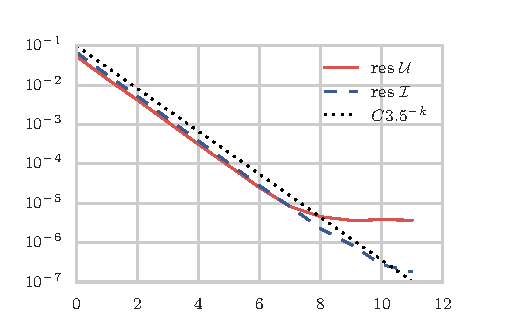
\includegraphics{figures/unloaded_error}
  \caption{\label{paper4:fig:unloaded_convergece_test}Convergence of the
    backward displacement method for the unloaded
    ($\mathrm{res}\;\mathcal{U}$) and loaded
    ($\mathrm{res}\;\mathcal{I}$) geometry.}
\end{figure}


\subsubsection{Convergence of the joint estimation of unloaded
  configuration and passive material parameters}
\label{paper4:sec:convergence_unloaded_material}

In this section we want to show that the iterative approach outlined
in Algorithm \ref{paper4:alg:unload_mat_bdm} is able to retrieve a known
material parameter under ideal circumstances. Further, we would like
to analyze the stability of the method with respect to noise in the
measurements.

A simple ellipsoidal geometry is inflated first to 0.6 kPa and then
to 1 kPa using known material parameters. Here we choose $a=3.1268$
kPa, $a_f = 1$ kPa, $b=1.0$ and $b_f=1.0$. At the first point with a
pressure of 0.6 kPa, the geometry is saved and will be used as the image-based
geometry. The second point, with the pressure at 1 kPa will represent
the end-diastolic state, and the cavity volume is computed.

We start the joint estimation with an initial guess for $a$ of 30
kPa. The relative error in the material
parameter is shown for each iteration in Figure
\ref{paper4:fig:unloaded_materror}. Here we also plot the chosen residual, which
is the relative difference in unloaded cavity volumes in two
successive iterations. We note that both of these residuals
converges at the same rate. 


\begin{figure}[htbp]
  \centering
  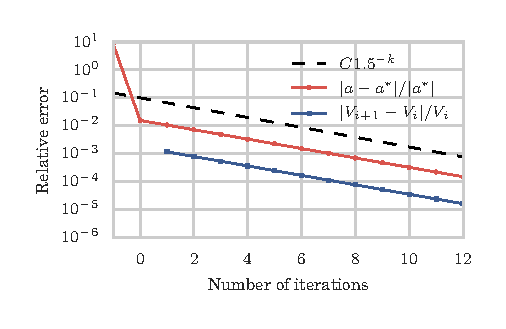
\includegraphics{figures/materror}
  \caption{\label{paper4:fig:unloaded_materror}Relative error in the material parameter for each iteration
  (red curve). The first point, at iteration -1 represent the error in
  the initial guess which is set to 30 kPa. The second point
  represents the error after estimating the material parameter by
  subtracting the offset. The remaining points represents the error
  after first unloading, and then optimizing with respect to the
  end-diastolic volume. Here we also show the chosen residual, which
  is the relative difference in unloaded cavity volumes (blue curve) and a
  supporting line showing the order of convergence. }
\end{figure}

To see the effect of noise in the data, we also test the method after
adding noise to the volume and pressure measurements. More specifically, we add
$\pm$ 0.1, 1, 5 and 10 $\%$ error to the pressure and volumes
independently. The resulting relative deviation from the exact value of the
material parameter is shown in Figure
\ref{paper4:fig:unloaded_materror_noise} for each iteration. We note that the
relative error in the resulting material parameter is of the same
order as noise level.

\begin{figure}[htbp]
  \centering
    \includegraphics{figures/materror_noise}
   \caption{\label{paper4:fig:unloaded_materror_noise}  Relative deviation from the
     exact value of the material parameter when noise is added
     to the measured volumes (left)
     and pressure (right). Noise of 0.1, 1, 5 and 10 $\%$
     is added and subtracted from the target volume and pressure, and
     the material parameter is estimated using Algorithm
     \ref{paper4:alg:unload_mat_bdm}. On the $y-$axis we show the
     relative deviation from the exact value, plotted against the number
   of iterations on the $x-$axis. }
\end{figure} 
% We want to test the accuracy of the proposed method for estimating
% material parameters and the unloaded configuration. To do this we 

% \begin{figure}[htbp]
%   \begin{subfigure}[t]{\textwidth}
%     \includegraphics[width=\textwidth]{../convergence_tests/unloaded_material_parameter_estimaton/material_parameter}
%     \caption{\label{paper4:fig:unloaded_material_parameter_value}} 
%   \end{subfigure}
%   \begin{subfigure}[t]{\textwidth}
%     \includegraphics[width=\textwidth]{../convergence_tests/unloaded_material_parameter_estimaton/material_parameter_error}
%     \caption{\label{paper4:fig:unloaded_material_parameter_error}} 
%   \end{subfigure}
% \caption{\label{paper4:fig:material_control}} 
% \end{figure}

\newpage


% \bibliographystyle{spbasic}
\bibliographystyle{plain}
\bibliography{chapters/paper4/bibliography}


%  LocalWords:  subendocardial

%%% Local Variables:
%%% mode: latex
%%% TeX-master: "../../main"
%%% End:




\backmatter

\end{document}

%%% Local Variables:
%%% mode: latex
%%% TeX-master: t
%%% End:
